% !TeX encoding = ISO-8859-1
% !TeX spellcheck = fr_FR
% !TeX root = book.tex
\documentclass[12pt, a4paper]{book}

\usepackage{graphicx}
\usepackage[margin=3cm]{geometry}
\usepackage[latin1]{inputenc}
\usepackage[T1]{fontenc}
\usepackage{xcolor}
%\usepackage[cyr]{aeguill}
\usepackage[french]{babel}
\usepackage{titlesec}
\usepackage{hyperref}
\usepackage{subcaption}
\usepackage{multicol}


%\usepackage{gentium}
\usepackage{lmodern}
\renewcommand{\familydefault}{\sfdefault}


\usepackage{eso-pic}

\newcommand\BackgroundPic{%
	\put(0,0){%
		\parbox[b][\paperheight]{\paperwidth}{%
			\vfill
			\centering 
			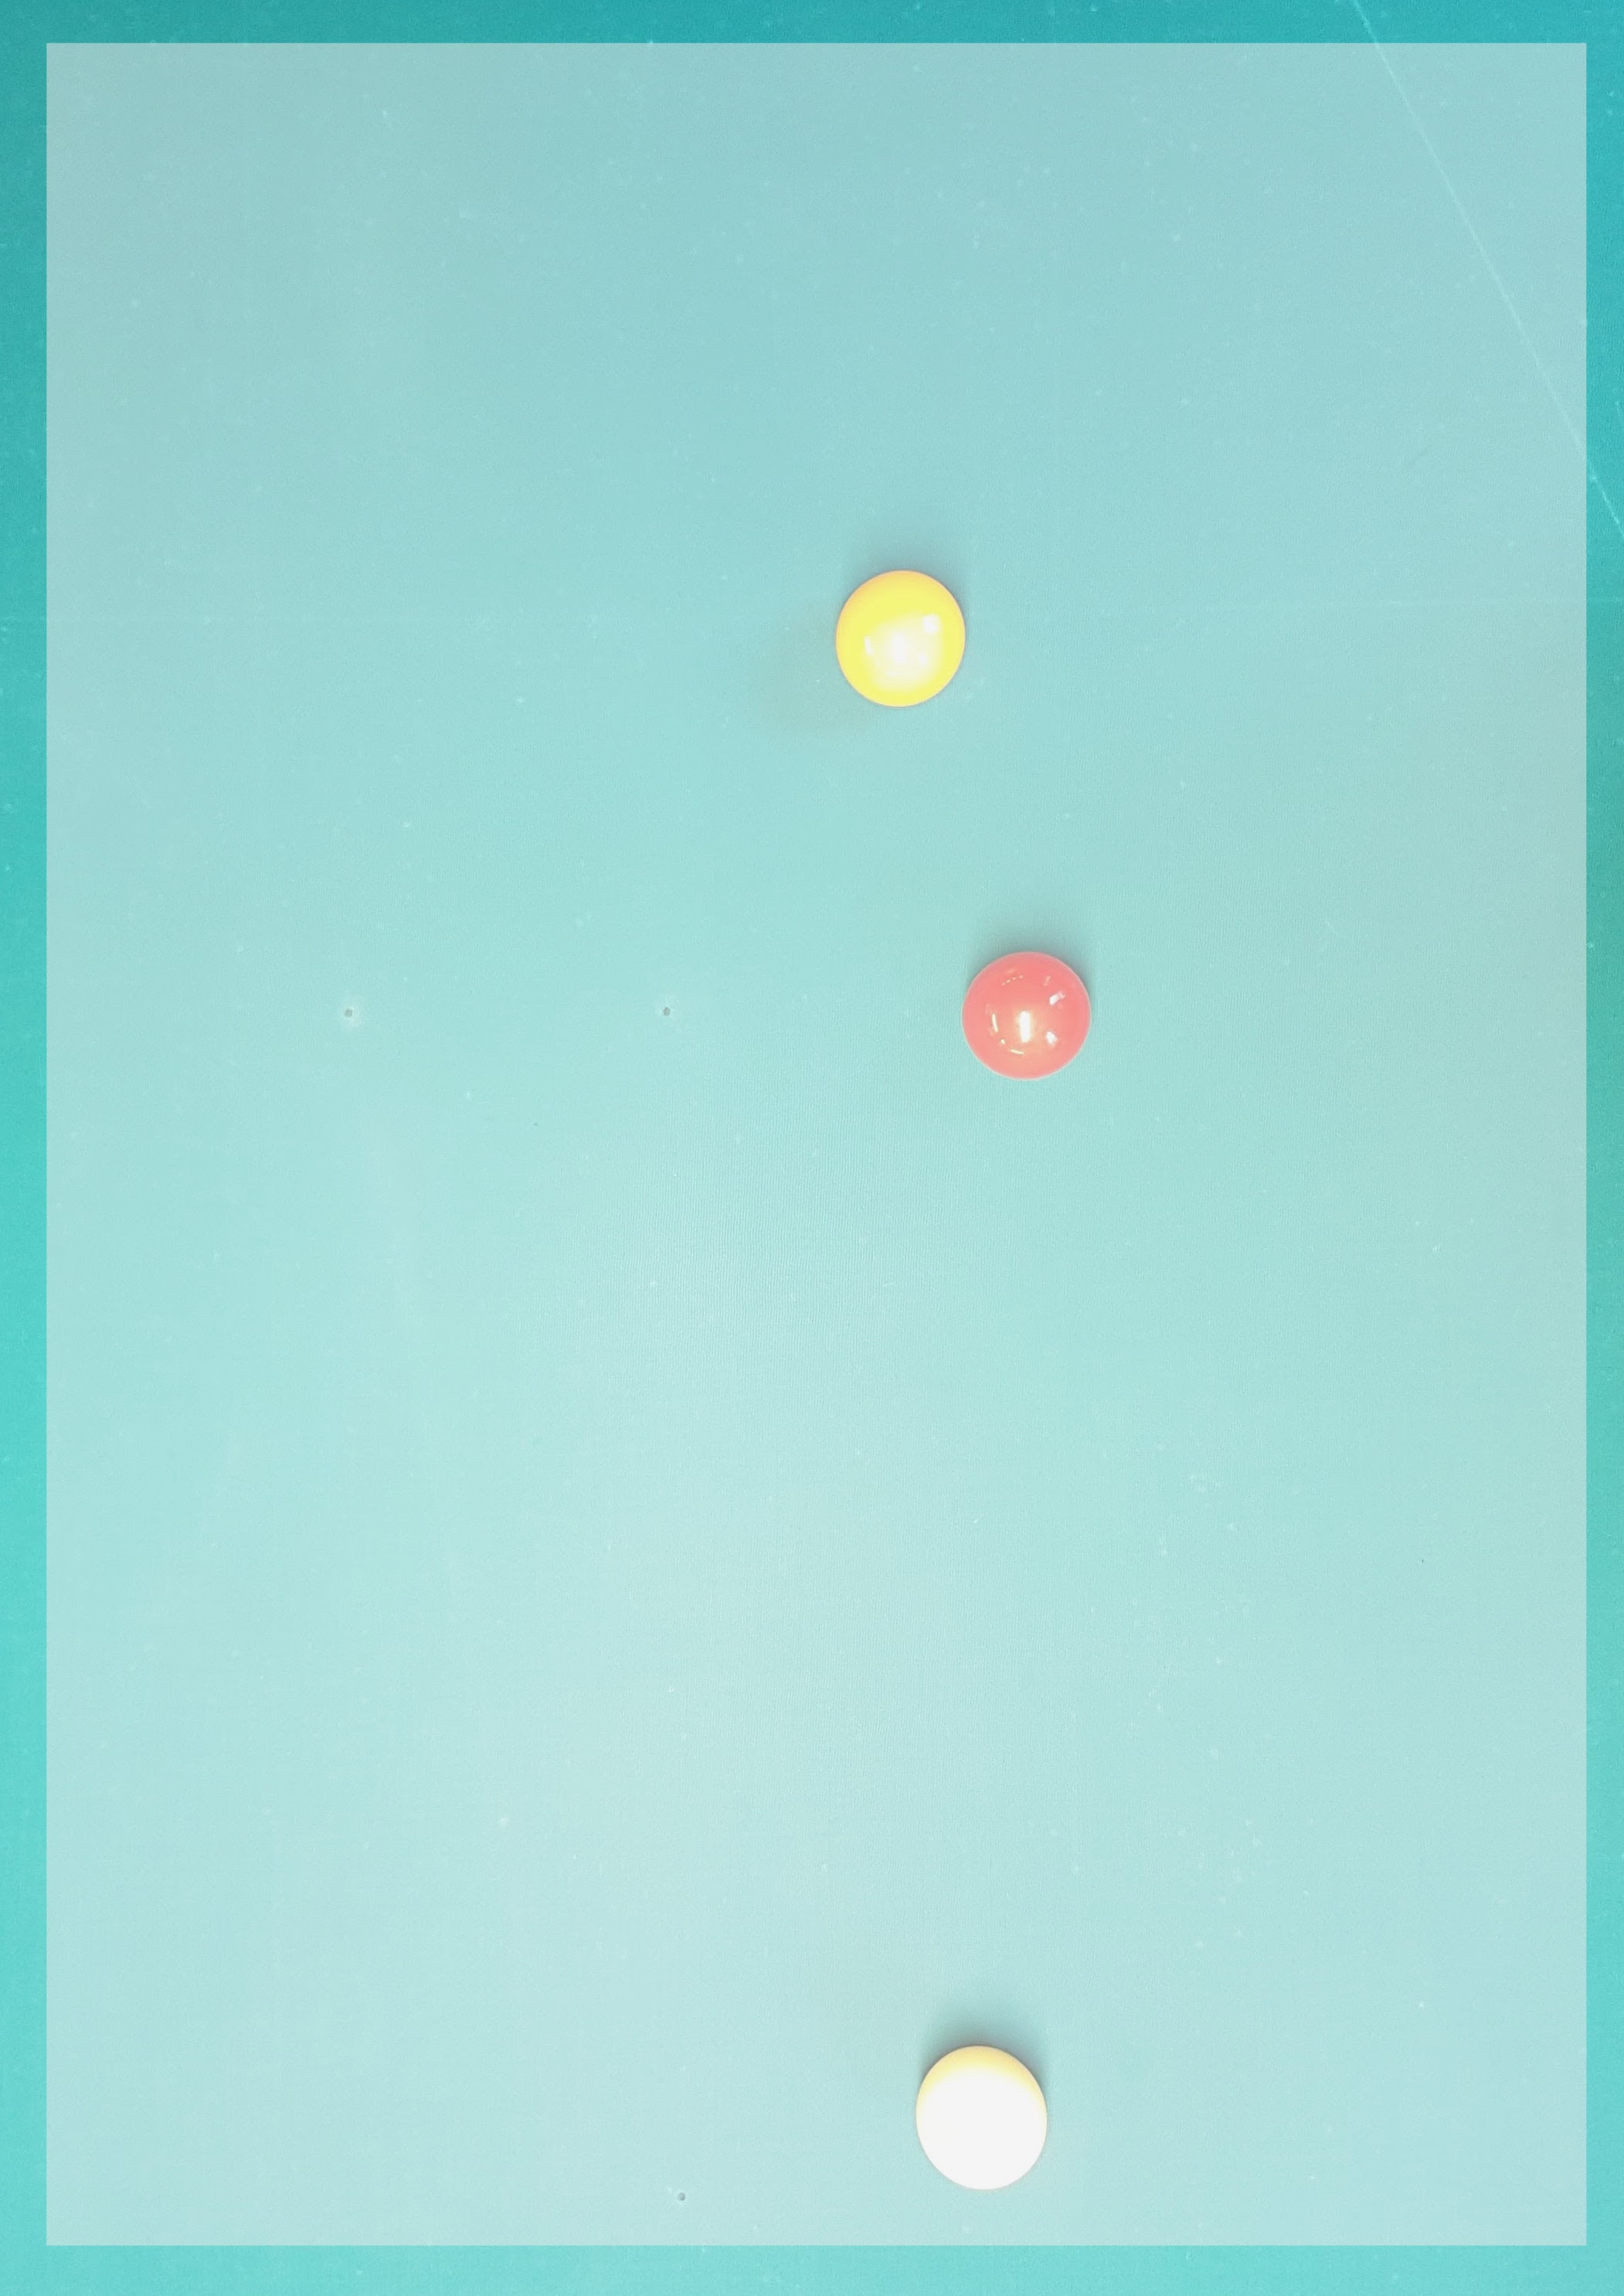
\includegraphics[width=\paperwidth,height=\paperheight,%
			keepaspectratio]{title_page_image.jpg}%
			\vfill
		}}}

%\renewcommand{\dbltopfraction}{0.9}	% fit big float above 2-col. text
%\renewcommand{\textfraction}{0.3}	% allow minimal text w. figs
%   Parameters for FLOAT pages (not text pages):
%\renewcommand{\floatpagefraction}{0.75}	% require fuller float pages
% N.B.: floatpagefraction MUST be less than topfraction !!
%\renewcommand{\dblfloatpagefraction}{0.75}	% require fuller float pages

\renewcommand{\thechapter}{\Alph{chapter}}%


\begin{document}
\AddToShipoutPicture*{\BackgroundPic}

\begin{titlepage}
	\thispagestyle{empty}
	\centering
	
	\textcolor{black}{\Huge{\bf Le billard sans peine ... \quad\quad \quad}}\\[5mm]
	\textcolor{black}{\Huge{\bf \quad \quad \quad ... ou presque.}}\\[5mm]
	
	\Large \textbf{Andr� Gal�re}
	
	\vspace{14cm}
	
	\textcolor{black}{\Large \textit{Le Billard constitue l'Art sup�rieur de l'anticipation.	Il ne s'agit pas d'un jeu mais d'un sport artistique complet qui n�cessite une bonne condition physique,
	le raisonnement logique du joueur d'�checs et le toucher du pianiste de concert.} Albert Einstein.}
	\vfill

\end{titlepage}


\noindent Images : Pascal Allegro.\\
Edition : Bertrand Corn�lusse.\\
Avril 2023.


\tableofcontents

\chapter{Tenir sa canne}

En pr�ambule, je tiens � signaler que le cours que j'ai con�u, s'adresse aux d�butants et ne constitue qu'une m�thode. Il y en a bien d'autres. Mon but est d'aider les amateurs de billard � am�liorer leurs performances, quelles que soient la hauteur de celles-ci. Si d'aventure, quelque dou� voulait atteindre les � hautes sph�res � il conviendrait de poursuivre au-del� avec un autre cours plus sp�cialis� et un autre professeur. Ce cours devrait permettre de passer de � rien � � excellence petit format au maximum et ne permet pas de t�ter certaines disciplines comme la bande et le trois bandes. 

% !TeX encoding = ISO-8859-1
% !TeX spellcheck = fr_FR

\newpage
\section{Position du joueur}

\subsection{Les pieds} 
Les pieds doivent �tre stables, l�g�rement �cart�s de mani�re � assurer une surface au sol la plus large possible (\autoref{fig:a01-a}).
Une bonne assise permet un bon �quilibre sans d�pense d'�nergie inutile et un bon positionnement face au jeu.

\subsection{ Les jambes} 
�galement �l�ments de stabilit�, elles doivent supporter le poids du corps uniform�ment. 
Jamais, une jambe seule ne doit supporter le poids du corps, sauf s'il est impossible de poser les deux pieds au sol ! Si on doit forcer sur une jambe pour garder l'�quilibre, cela peut �tre une source d'impr�cision voire d'erreur de jugement. Les jambes doivent �tre l�g�rement fl�chies, comme si on �tait pr�t � s'asseoir sur une chaise. 
Cette position permet une orientation correcte du tronc. 
Au d�but, elle semblera un peu p�nible. 
Avec le temps, il sera possible d'am�nager des corrections de confort sans alt�rer le jugement du joueur : avancer un
pied, s'aplatir le tronc sur la canne ou raidir une jambe. \'A chacun de voir, mais retenons qu'une assise souple est toujours pr�f�rable � une assise raide.

\subsection{Le tronc} Le tronc est face � la direction choisie,
fermement stabilis�, inclin� vers l'avant. Id�alement,
le menton, le nombril et la bille 1 devraient �tre parfaitement align�s.
Seul un contorsionniste pourrait y arriver mais il faut tenter de
s'en rapprocher. Dans ses conditions id�ales, la vue du
joueur est situ�e � la verticale de cette droite (\autoref{fig:a01-b}).

\begin{figure}
	\centering
	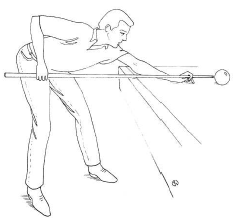
\includegraphics[width=0.7\linewidth]{A/imagesA/A01-a}
	\caption{Position du corps.}
	\label{fig:a01-a}
\end{figure}
\begin{figure}
	\centering
	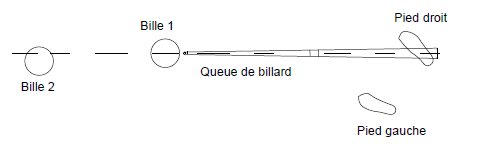
\includegraphics[width=0.7\linewidth]{A/imagesA/A01-b}
	\caption{Vue du dessus.}
	\label{fig:a01-b}
\end{figure}




% !TeX spellcheck = fr_FR
% !TeX encoding = ISO-8859-1

\newpage
\section{Position des Mains}

\subsection{La main arri�re} C'est elle qui joue ! Un gaucher a la main gauche � l'arri�re, un droitier, la main droite. Elle sert principalement � soutenir la canne, sans la presser, sans la retenir, sans la serrer. C'est cela qu'il convient d'avoir en t�te au d�but. Plus tard, nous verrons que la tenue arri�re poss�de une palette de coups et de positions. Pour l'heure, contentons-nous de bien retenir que la main arri�re soutient la canne, la fait coulisser d'avant en arri�re et d'arri�re en avant (limage), avant de porter le coup dans un mouvement r�gulier, souple, et rectiligne, bien dans le prolongement de la canne, afin d'ajuster le tir exactement, sans balancement lat�ral ni vertical. Le plus souvent possible, la canne sera mise en mouvement le plus horizontalement possible. 

\subsection{La main avant} La main avant sert � stabiliser, sans la retenir, le talon de la canne, de mani�re que celui-ci puisse coulisser sans retenue et sans jeu lat�ral. La main avant ne joue pas ! Elle ne peut pas bouger quand on porte le coup ! Elle soutient la fl�che. 

\begin{itemize}
	\item Pos�e sur le tapis, �carter bien franchement les trois doigts c�t� petit doigt, afin d'assurer une bonne assise parfaitement stable et solide (\autoref{fig:a02-3}). Le pouce sert d'appui � la canne pendant que l'index, repli� par-dessus, figure un petit pont qui va servir de serre-joint � la canne, suffisamment ferme pour emp�cher le flottement lat�ral et assez l�che pour permettre le coulissement sans retenue. De cette fa�on, on joue en position basse. Le rapprochement par arc de cercle des trois doigts de base fait passer le tir de la position basse � mi-hauteur puis � la position haute quand les doigts sont compl�tement repli�s. Pour les joueurs � � petite main �, la position haute ressemble � un poing ferm�.
	\item Pos�e sur la bande ou le bois du billard (\autoref{fig:a02-4}) : lorsque la bille � frapper est trop pr�s de la bande, emp�chant de poser la main sur le tapis, poser la canne sur le bois du billard et poser l'index et son voisin de chaque c�t� de la fl�che, doigts tendus. Serrer l�g�rement ces deux doigts de mani�re � emp�cher toute oscillation lat�rale. Dans cette position, on ne peut jouer qu'en position haute. 
\end{itemize}

\begin{figure}
	\centering
	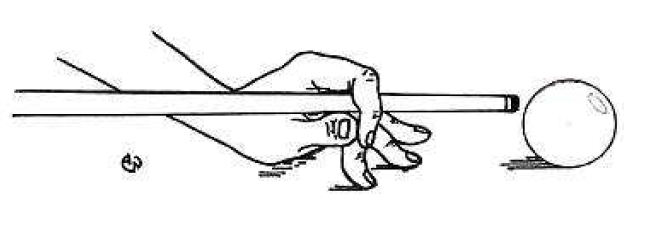
\includegraphics[width=0.48\linewidth]{A/imagesA/A02-3}
	\caption{Bille loin d'une bande.}
	\label{fig:a02-3}
\end{figure}
\begin{figure}
	\centering
	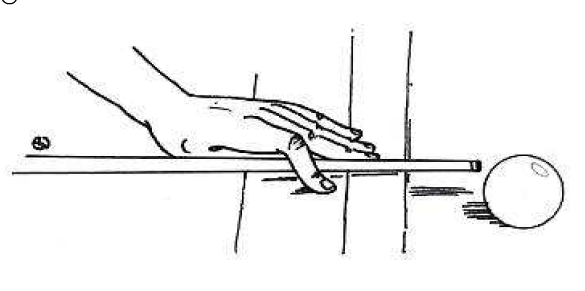
\includegraphics[width=0.48\linewidth]{A/imagesA/A02-4}
	\caption{Bille proche d'une bande.}
	\label{fig:a02-4}
\end{figure}

\noindent Remarques : 
\begin{itemize}
	\item Les deux doigts tendus sur le bois interdisent une position basse (b-2). Cependant, s'il est n�cessaire de jouer � en bas �, on devra lever le talon � l'arri�re et poser la main avant classiquement comme sur le tapis (a-1). 
	\item D'autres positions, moins fr�quentes ou plus sp�ciales, seront expliqu�es ult�rieurement. 
\end{itemize}

%TODO V�rifier 
Pour vous entrainer (\autoref{fig:a02-1}), placer les trois billes dans un coin, et frappez les de mani�re � les envoyer dans le triangle hachur� en trois bandes. La derni�re doit partir avant que la premi�re ne s'arr�te. 
\begin{figure}
	\centering
	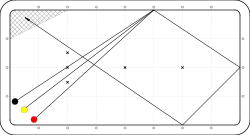
\includegraphics[width=\linewidth]{A/imagesA/A02-1}
	\caption{Envoyer les trois boules dans le coin.}
	\label{fig:a02-1}
\end{figure}

Un autre exercice (\autoref{fig:a02-2}) consiste � frapper la bille 2 pleine bille, pour que les deux billes se rencontrent apr�s le rebond de la bille 2 sur la petite bande. Cela permet d'apprendre � frapper bien droit.
\begin{figure}
	\centering
	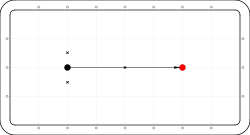
\includegraphics[width=\linewidth]{A/imagesA/A02-2}
	\caption{Frapper droit.}
	\label{fig:a02-2}
\end{figure}


% !TeX spellcheck = fr_FR
% !TeX encoding = ISO-8859-1

\newpage
\section{L'effet : position de la canne}

La canne est compos�e principalement d'un talon, d'une fl�che, d'une v�role et d'un proc�d�. Nous jouons en projetant le proc�d� (le cuir) sur la bille. La 1 est la bille avec laquelle nous jouons, la 2, celle qui sera percut�e la premi�re par la 1 et enfin la 3, la derni�re touch�e par la 1. Le jeu consiste, en � libre �, � frapper la 1 avec le cuir de notre fl�che de mani�re qu'elle aille percuter les deux autres billes. 

Chaque � coup � r�ussi est compt� un point par l'arbitre et permet de continuer le jeu tant qu'on r�ussit, pouvant ainsi � marquer � plusieurs points avant de passer la main. Si on rate au premier essai, l'arbitre compte z�ro et on doit passer la main � l'adversaire directement. Une partie se joue en un certain nombre de points � r�aliser allant de la huiti�me cat�gorie (30 points) � l'excellence (300 points). 

De mani�re � ex�cuter une carambole correspondant � une vision directe, il est important pour la majorit� des points que la canne soit tenue le plus pr�s possible de l'horizontale. Avant tout : limer. La pr�cision est essentielle. Pour cela, il conviendra de rep�rer sur la bille, des endroits bien d�termin�s qui, avec un coup toujours le m�me, donnera un r�sultat, toujours le m�me (\autoref{fig:a03-1}). 
Si on partage la 1 par deux axes, l'un vertical et l'autre, horizontal, on partage le cercle visible de la bille en 4 zones ou secteurs. Nous d�gageons ainsi, 9 prises de billes pr�cises � savoir : 

% TODO v�rifier figure d'Andr�.
\begin{itemize}
	\item Au croisement des deux axes pr�cit�s ou centre bille ou au milieu de la distance entre le centre et le haut ou au milieu de la distance entre le centre et le bas, soit sur l'axe vertical : on joue sans effet (la bille ne tourne pas sur elle-m�me pendant sa translation). 
	\item Jouant au centre de la zone 1, on imprime un effet � gauche faible. Pendant sa translation, la bille tourne sur elle-m�me faiblement dans le sens des aiguilles d'une montre. 
	\item Le coup port� au milieu entre le centre et l'extr�mit� gauche (ou au milieu entre le centre et l'extr�mit� droite, donc sur l'axe horizontal, imprimera un effet important. 
	\item 	Enfin, au milieu du secteur 3, l'effet port� sera tr�s important. 
	\item 	Les zones 2 et 4 sont �quivalentes aux zones 1 et 3, l'effet est port� � droite. 
\end{itemize}
\begin{figure}
	\centering
	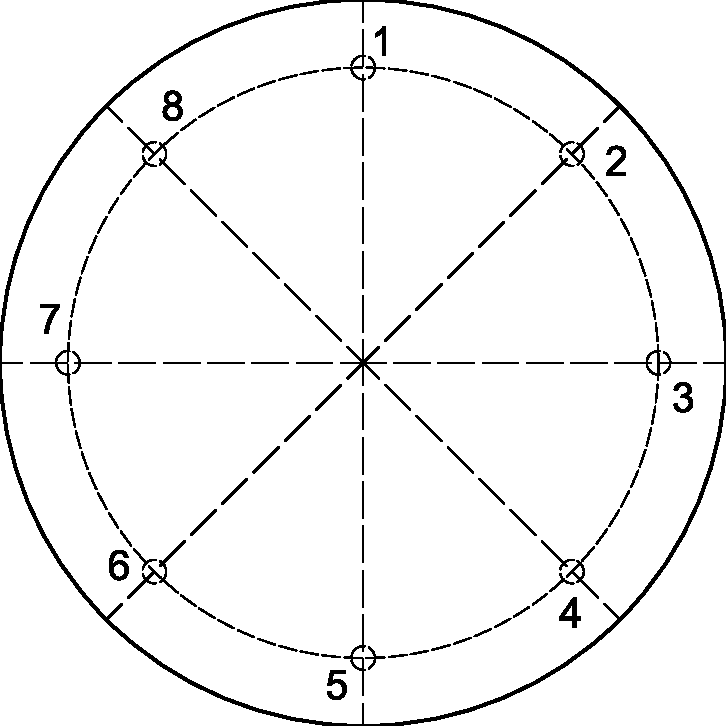
\includegraphics[width=0.4\linewidth]{A/imagesA/A03-1.pdf}
	\caption{Les positions de frappe sur une bille.}
	\label{fig:a03-1}
\end{figure}

\begin{figure}
	\centering
	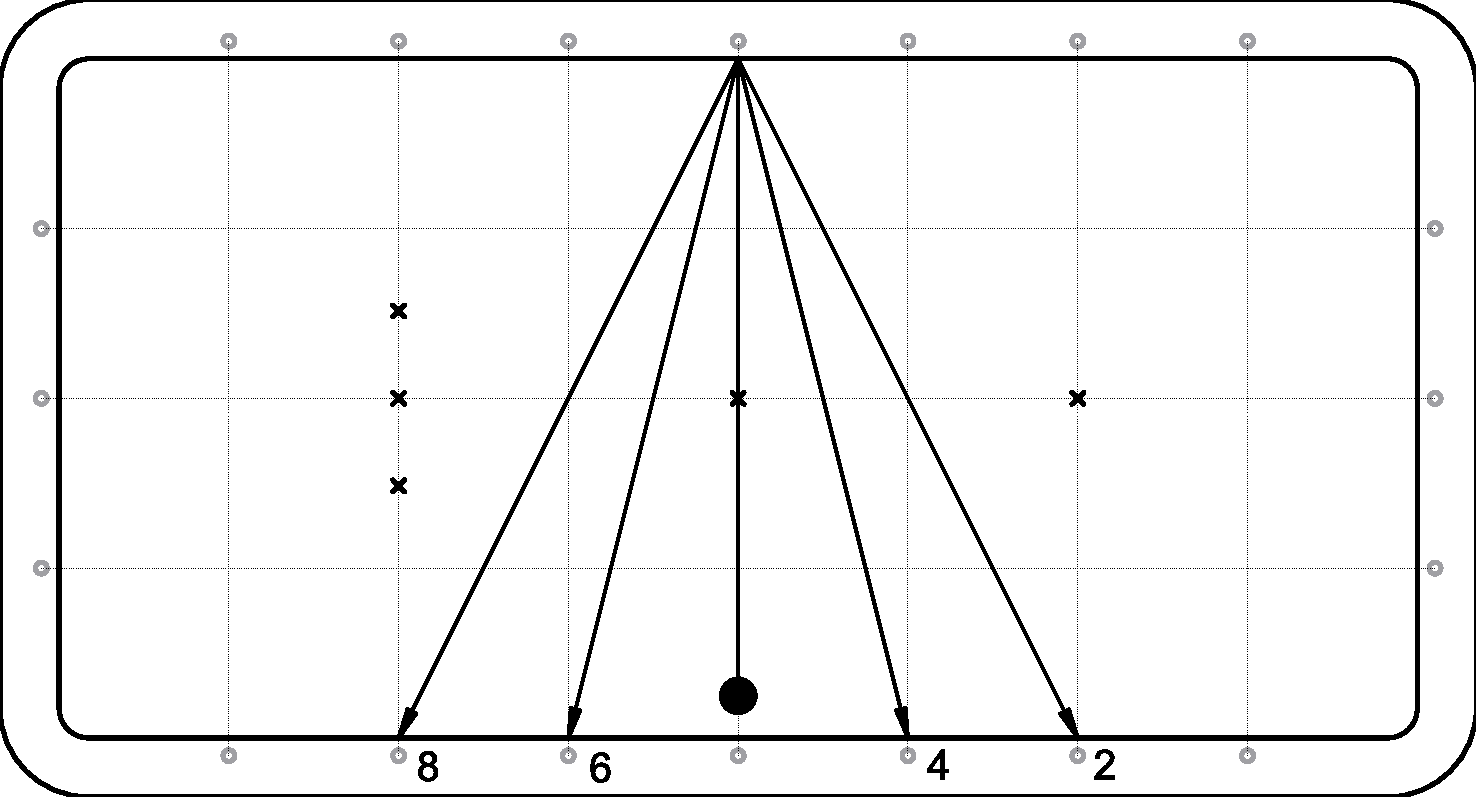
\includegraphics[width=0.95\linewidth]{A/imagesA/A03-2.pdf}
	\caption{Exercice sur l'effet � gauche et � droite. Essayez de doser l'effet lat�ral en partant du centre du billard et en suivant la perpendiculaire � la grande bande afin d'atteindre les points 2, 4, 6 et 8.}
	\label{fig:a03-2}
\end{figure}
\noindent Essayez l'exercice de la \autoref{fig:a03-2}.
\begin{itemize}
\item L'effet produit son << effet >> seulement (ou � peu pr�s) lorsqu'il rencontre un obstacle, par ex.la bande. 
\item On appellera � bon effet �, celui qui a tendance � prolonger le mouvement de la bille o�, apr�s contact, la bille se rapproche de la bande.
\item On appellera � effet contraire �, celui qui a tendance � contrecarrer le mouvement de la bille, o�, apr�s contact, la bille se rapproche de la perpendiculaire � la bande. 
\item Cette d�signation de bon effet ou effet contraire est pure convention pour cet expos�.  D'autres d�signent les choses autrement : question de convention afin de se comprendre par la suite. 
\end{itemize}
\clearpage


% !TeX spellcheck = fr_FR
% !TeX encoding = ISO-8859-1

\section{L'effet}

Le � bon effet � prolonge le mouvement de la bille, l' � effet contraire
� ralentit le mouvement de la bille, voir \autoref{fig:a04-1}. L'effet ne produit son effet qu'en rencontrant un obstacle.
Les changements de direction dus � l'effet seront d'autant plus
importants qu'on jouera bas de bille.

Fig l : L'effet est contraire sur la bille 2 et bon sur la bande : la
1 aura tendance � s'�tendre le long de la bande donc � s'�carter de la
perpendiculaire au point d'impact sur la bande, ou, si l'on pr�f�re :
l'angle de r�flexion sera plus grand que l'angle d'incidence.

Fig 3: L'effet est bon sur la bille 2 et contraire sur la bande. La 1 aura tendance � retenir son mouvement donc � se rapprocher de la
perpendiculaire � la bande au point d'impact : l'angle r�fl�chi sera
plus petit que l'angle d'incidence.

Fig 2 : Cette figure montre le ph�nom�ne d'engrenage de l'effet. Tout se passe comme si les billes �taient des roues dent�es. Quand la 1
rencontre la deux, elle lui donne une partie de son �nergie sous forme
de rotation dont le sens sera inverse � celui d'origine ... comme avec
les engrenages. 
\begin{itemize}
\item Ainsi, si nous imprimons � la 1 une rotation gauche, au moment de l'impact avec
la 2, elle imprimera � celle-ci une rotation droite. L'effet de la 2
sera plus faible que celui d'origine mais pas du tout inexistant. On
constatera le ph�nom�ne de deux fa�ons : la 2 est l�g�rement d�vi�e dans
le sens de l'effet de la 1 et au toucher de la premi�re bande, elle aura
une d�viation correspondant � l'effet inverse de la 1.
\item C'est en � soutenant � bien son � coup � qu'on imprimera une
part plus importante d'effet � la 2. Ce ph�nom�ne d'engrenage est
capital pour rappeler des positions qui sans cela, seraient perdues. La
bonne compr�hension de ce ph�nom�ne facilitera grandement l'�tude du jeu
de rappel.
\end{itemize}

\begin{figure}[htb]
	\centering
	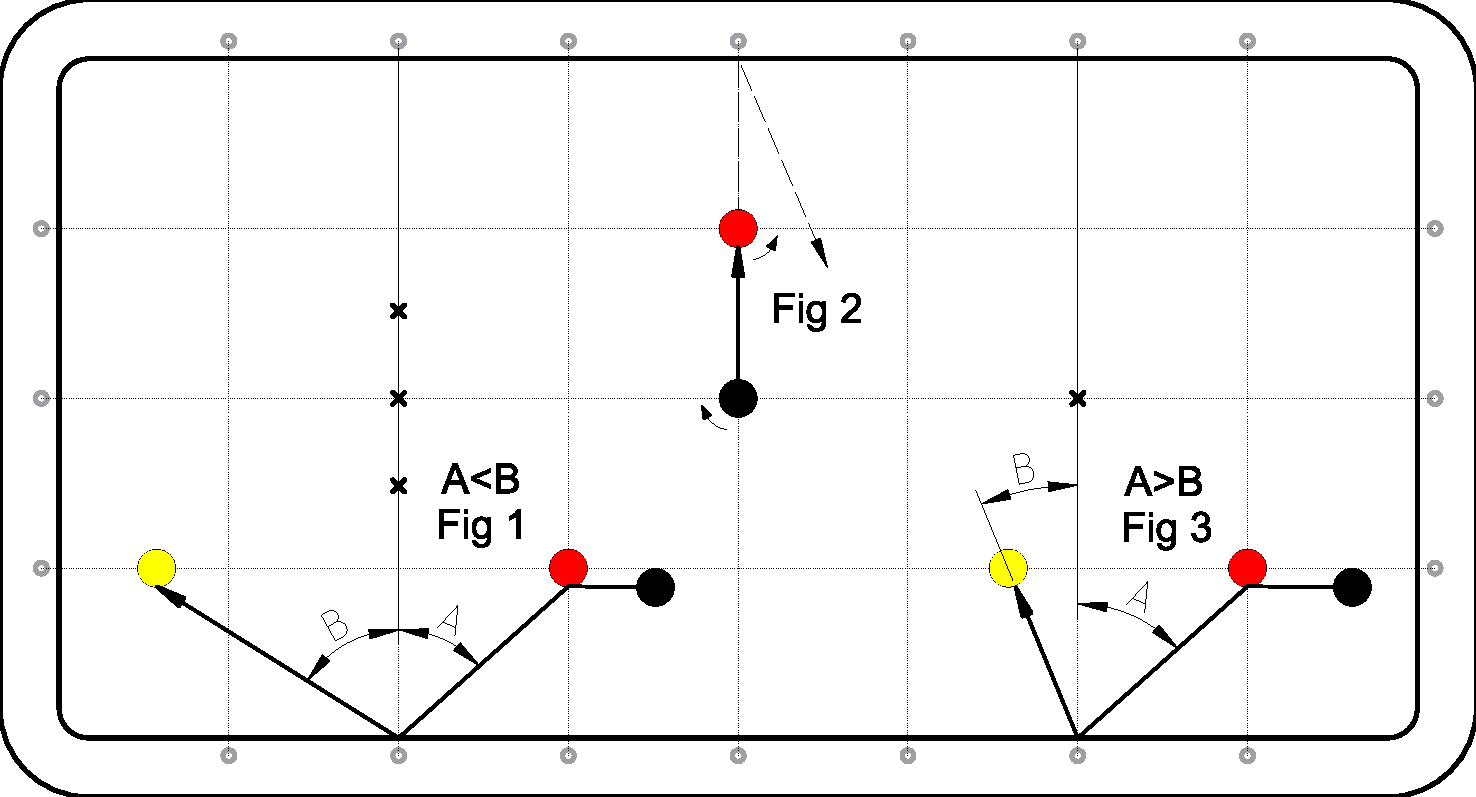
\includegraphics[width=\linewidth]{A/imagesA/A04-1.pdf}
	\caption{Effet contraire, engrenage et bon effet.}
	\label{fig:a04-1}
\end{figure}

\clearpage
% !TeX spellcheck = fr_FR
% !TeX encoding = ISO-8859-1

\section{Le coul�}

Le coul� (\autoref{fig:a05-1}) est un des points de base du billard. Il permet de r�aliser des caramboles dites <<non naturelles>>.

La bille 2 est plac�e de telle sorte que la finesse est impossible ou
tr�s difficile. D'abord examinez si le coul� est possible. Celui-ci
consiste � faire prolonger le mouvement de la 1 vers l'avant apr�s avoir
heurt� la 2, parfois presque la m�me direction comme si la 1 voulait
suivre la 2. Mais pour que le point soit possible, la direction 1-2 ne
peut pas � couper � l'image de la 3, sinon apr�s le coup, la 2 risque de
toucher la 3 et l'�carter emp�chant ainsi la 1 de r�aliser le point.
Pour v�rifier cela : tracez une ligne imaginaire tangente aux billes 1
et 2, c�t� de la 3 et si cette ligne ne rencontre pas la 3, le point est
possible.

Le coul� � normal � se joue presque plein sur la 2, coup prolong�, haut
de bille, coup accompagnant la 1 dans son mouvement. Le d�calage de la
prise de la 1 se situe du c�t� de la 3. La masse non prise de la 2,
correspond � la touche qu'on aurait d� n�gocier si on avait tent� la
finesse. Autrement dit, il faut prendre � toute � la 2 moins ce qu'on
aurait pris en finesse. Une l�g�re d�portation sera donc appliqu�e du
c�t� de la 3. Lorsque la prise de la deux est particuli�rement proche de
la bille pleine, on parlera d'une nuance droite pour une d�portation
vers la droite et d'une nuance gauche pour une d�portation vers la
gauche.

Le coup � normal � se porte sur l'axe vertical, donc sans effet.
Beaucoup de joueurs croient faciliter le coul� en appliquant un effet
inverse � la d�portation. Cela est pure l�gende. L'effet impliqu� jouera
dans le cas o� nous coulons vers la bande ou bien imprimera un effet
inverse � la 2. L'effet n'influence pas le mouvement de la 1 ... ou si
peu.... Il rassure, c'est tout. En fait, l'effet inverse rapproche la 2
du champ de la 3, l'effet du bon c�t� l'�carte.

Nous allons nous servir de cette qualit�. Si la tangente cit�e plus haut
� mord � un peu la 3, sans exag�ration, il sera encore possible de
r�aliser le coul�. On appliquera un effet du c�t� de la d�portation et
la 2 s'�cartera du chemin de la 3 (� essayer).

Si la tangente passe trop pr�s du centre, la d�viation de la 2 ne sera
jamais suffisante pour �viter le choc avec la 3. Il conviendra d�s lors
de choisir une autre solution.
\begin{figure}[htb]
	\centering
	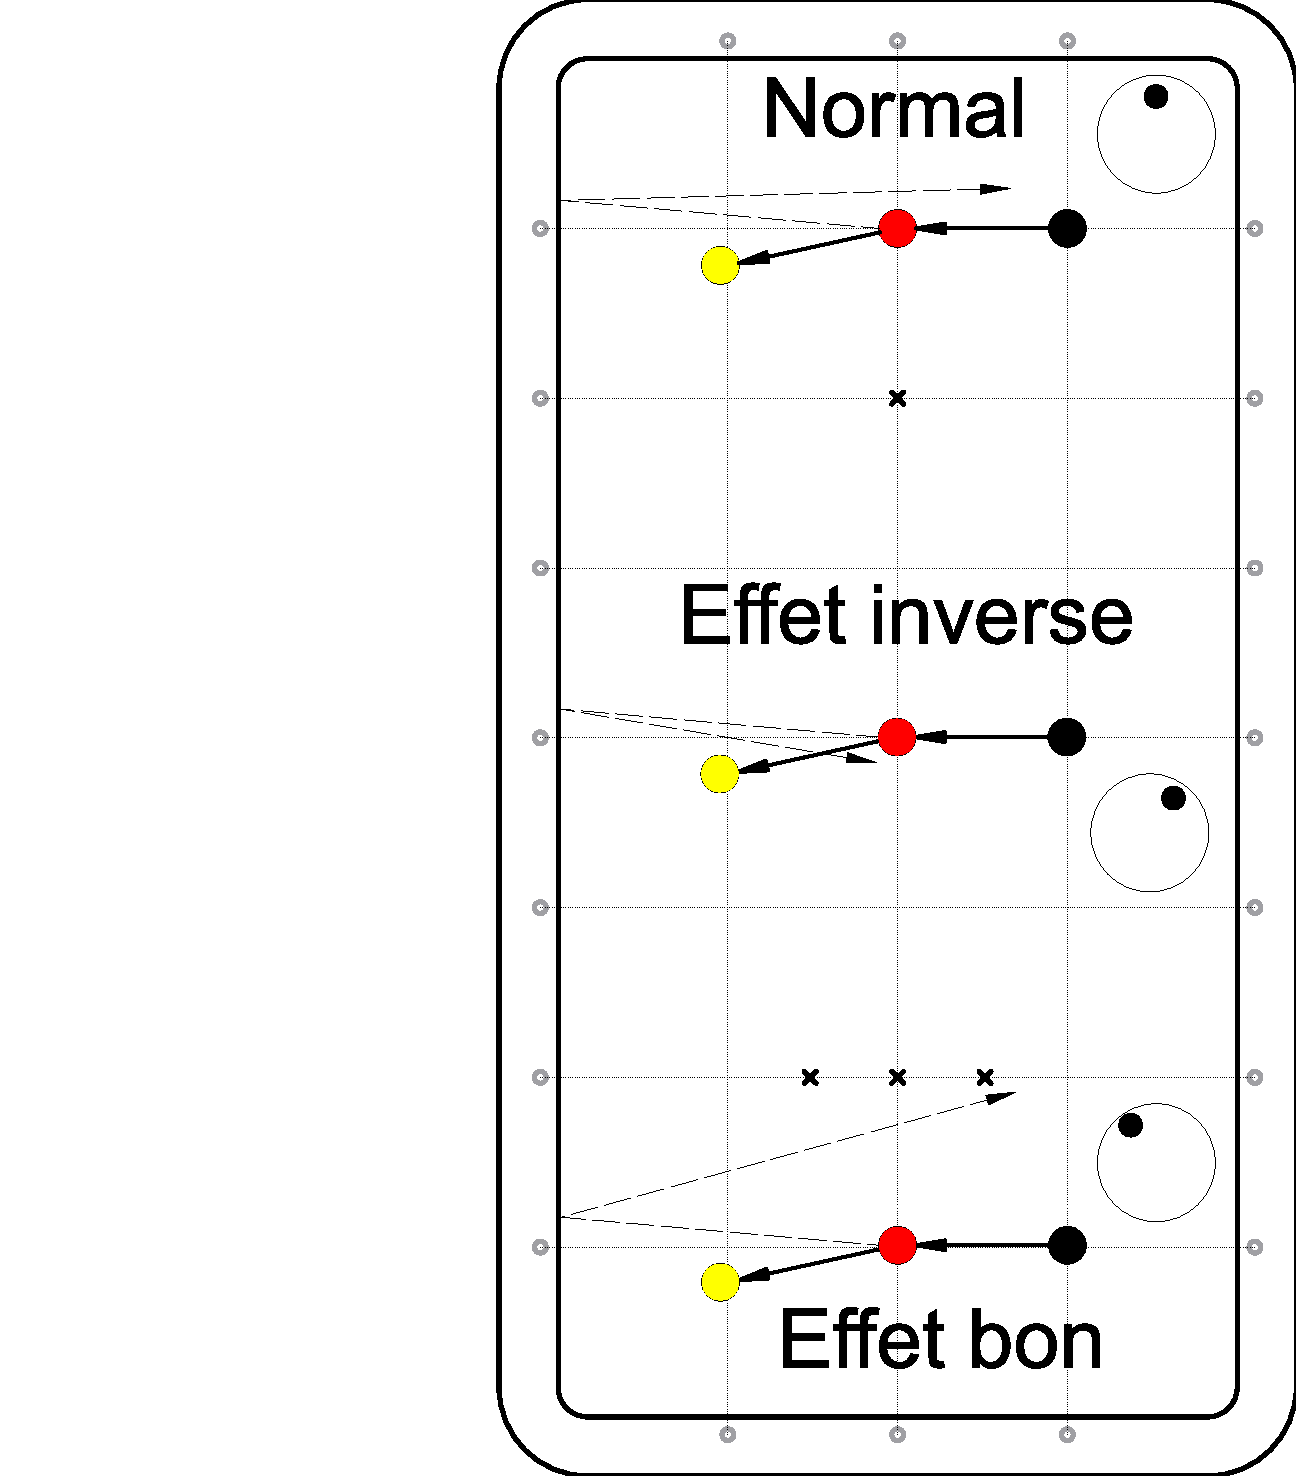
\includegraphics[width=0.85\linewidth]{A/imagesA/A05-1.pdf}
	\caption{Le coul�.}
	\label{fig:a05-1}
\end{figure}
\clearpage

% !TeX spellcheck = fr_FR
% !TeX encoding = ISO-8859-1

\section{Le r�tro}

Le r�tro est aussi un point de base au billard. Sa r�alisation est
facile pour un joueur aguerri mais ardu pour un d�butant. Il faudra
s'acharner jusqu'� ce que la � m�canique � devienne une <<�vidence>>.

Le r�tro est le contraire du coul�. La bille 1 revient sur ses pas en
direction de la 3, apr�s avoir touch� la 2. Il se joue bille basse, coup
allong� et m�me accompagnant, l�che et sans forcer. La main avant est
ferme et laisse une fl�che courte pour les petits d�placements et une
fl�che longue pour les longs. La main arri�re ne serre pas le talon et
se place le plus loin possible pour les longs d�placements et se
rapproche de l'�quilibre de la canne pour les petits points. La grosseur
de bille est la m�me que pour le coul� mais on y voit bien plus mal. Son
estimation ne sera pas chose ais�e aussi, nous allons utiliser un truc.

Consid�rons la fig 2 et voyez l'angle form� par les billes 1, 2 et 3,
sommet en 2... Tra�ons la bissectrice de cet angle qui coupe la surface
de la 2 au point I. Il suffit (hum...) de jouer sur ce point I et le
tour est jou�. Facile � dire car le point I est le point de touche et
pas celui de la vis�e mais rien n'est perdu car les billes sont des
miroirs sph�riques donc si nous nous positionnons pour jouer un r�tro,
nous allons voir dans la 2 l'image de la 3 ... et en visant cette image,
nous allons toucher au point I recherch�.

Merveille de la g�om�trie sph�rique !

Nous n'avons donc plus besoin de nous torturer pour mesurer la grosseur
de bille ... si la 2 est la rouge. Nous voyons bien l'image et m�me si
la 3 est �loign�e, son image est encore un petit point qu'on peut
apercevoir. Malheureusement, si la 2 est la blanche, nous ne voyons plus
l'image de la 3. Il conviendra de s'entra�ner ferme pour se � mettre
dans l'�il � cette fameuse grosseur de bille. Tout ceci est un truc et
n'est valable seulement que si on ne fait pratiquement intervenir que
les masses des billes c�d : bille basse, sans effet, p�n�tration moyenne
; force moyenne et main arri�re en position moyenne.

Attention ! la position et la tenue de la canne par la main arri�re sont
capitales. Afin d'assurer un bon retour de la 1, la main arri�re ne doit
que soutenir la canne, sans la presser. Pour ce coup, � la limite, on
pourrait se passer de cette main, elle est presque inutile. Il ne s'agit
pas d'une contradiction : la main arri�re est indispensable mais elle
doit se faire l�g�re.... presque gracieuse...

Remarque : Il y d'autres trucs mais c'est celui-ci que je pr�f�re... Il
a l'avantage, je crois, de forcer le joueur � toujours produire le m�me
coup ce qui, plus tard, lui permettra de bien le dominer, donc de le
varier et de lui permettre de dominer le mouvement de la 2 autant que
celui de la 1, donc de � construire � son jeu.

\begin{figure}[htb]
	\centering
	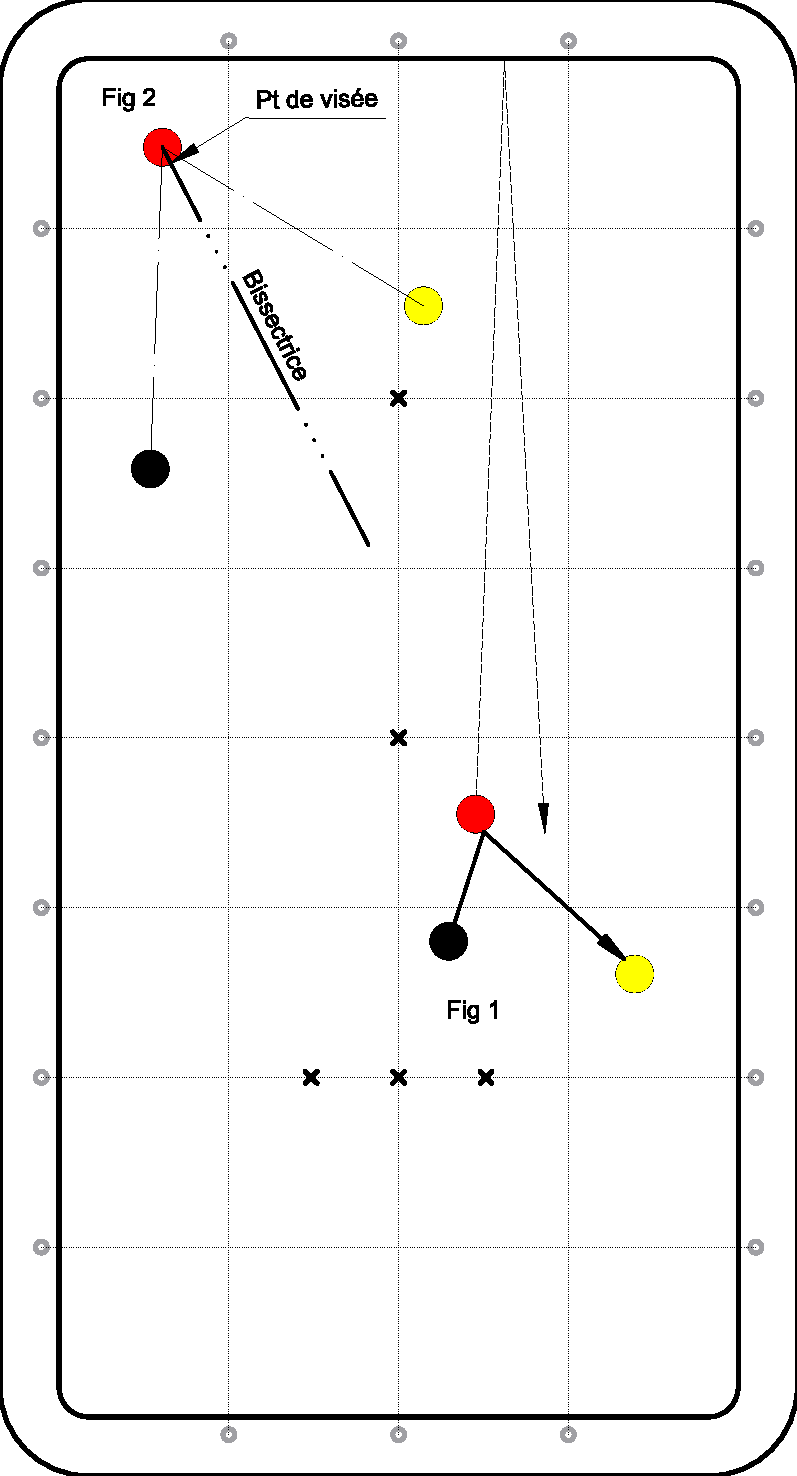
\includegraphics[width=0.85\linewidth]{A/imagesA/A06-1.pdf}
	\caption{Le r�tro}
	\label{fig:a06-1}
\end{figure}
\clearpage

% !TeX spellcheck = fr_FR
% !TeX encoding = ISO-8859-1

\section{Le 45�}

Ce point est particuli�rement important dans la mesure o� il constitue
une r�f�rence pour beaucoup de figures. Une fois acquis, il ne peut plus
�tre rat� (!). Il est facile. En cas d'�chec, notre ?il ou notre
position est responsable, voire notre distraction...

Il suffit de jouer en demi-bille la 2 du c�t� de la 3. � Prendre � une
demi-bille, c'est pousser la 1 en direction de la 2 de mani�re que, dans
son mouvement, la moiti� de la masse de la 1 co�ncide avec la moiti�
oppos�e de la masse de la 2... Pour une vis�e pr�cise, la 1 est prise au
centre bille, avec comme point de vis�e, la tangente � la 2. Il suffit
pour cela, une fois bien positionn�, de placer dans � sa vis�e �, le
bord de la 2 au milieu de l'image de la mouche de la fl�che.

Apr�s l'impact, la 1 ferait un angle de 45� si nous �tions dans un
espace � trois dimensions et sans frottement et si les billes 1 et 2
�taient en mouvement libre l'une vers l'autre et � vitesse �gale. Mais
comme nous sommes avec des volumes glissant sur un plan et qu'en plus le
mobile percuteur est en mouvement quand il s'�crase sur sa cible fixe et
... qui va se d�rober, l'angle est un peu inf�rieur, jusqu'� 40� si la
canne est tenue haute comme pour couler et jusqu'� 50� si la canne est
soutenue l�g�rement basse.

Retenons qu'une demi-bille a pour r�sultat un angle de 45�. Il y a une
erreur mais petite. En plus avec l'habitude, la merveilleuse m�canique
humaine va ajuster sans peine, ces petites diff�rences.

\begin{figure}[htb]
	\centering
	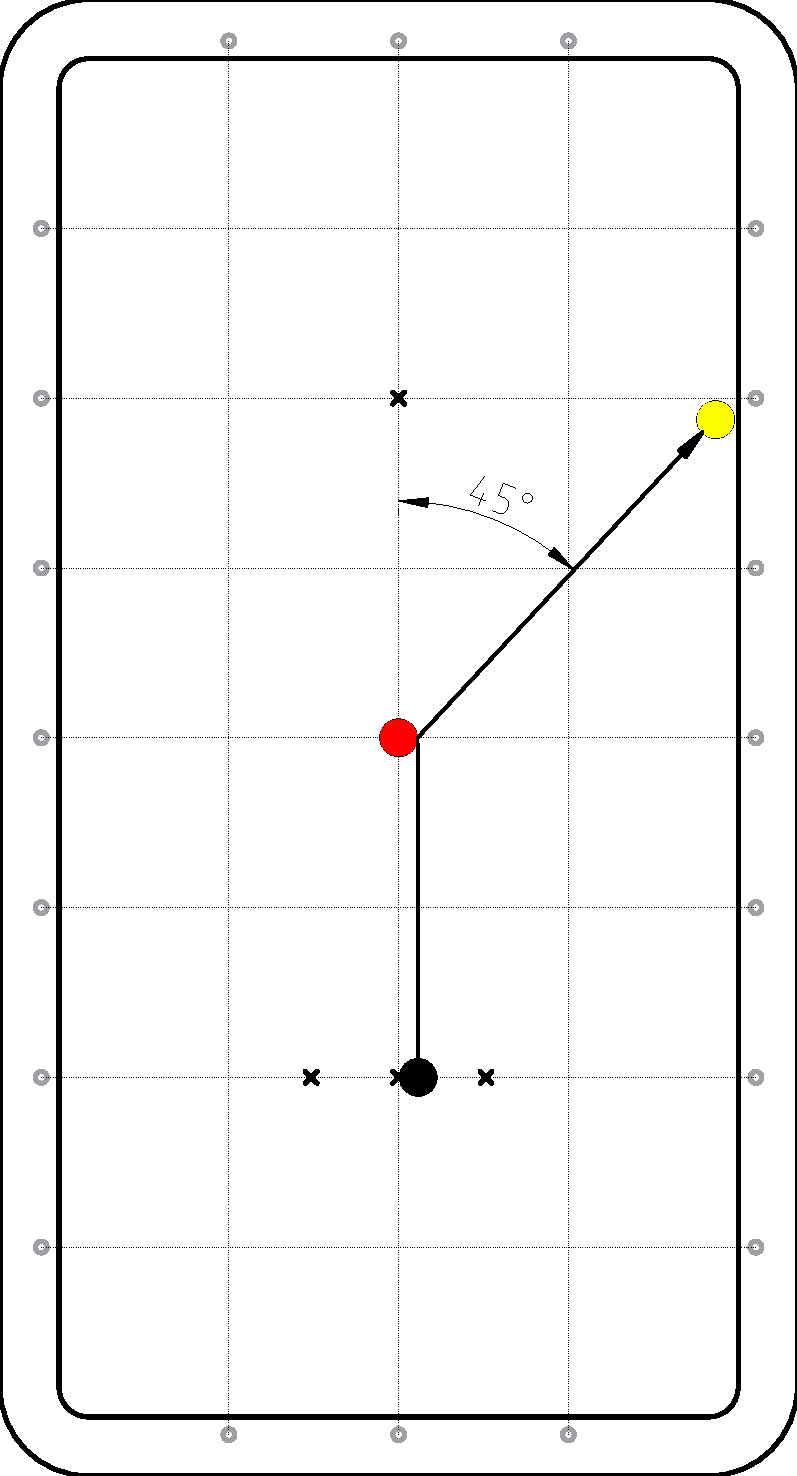
\includegraphics[width=0.85\linewidth]{A/imagesA/A07-1.pdf}
	\caption{Le 45�}
	\label{fig:a07-1}
\end{figure}
\clearpage

% !TeX spellcheck = fr_FR
% !TeX encoding = ISO-8859-1

\section{Le 90�}

Le 90� ou angle droit constitue un pas important � franchir pour le
d�butant. Bien travaill�, ce point devient facile, croit-on... M�fiance,
il est plein de nuance. Les � sp�cialistes � diront qu'on peut r�aliser
un angle droit aussi bien bon effet que contraire, qu'une prise de bille
pleine ou fine, voire superfine. Nous nous bornerons ici, � une m�thode,
laissant pour le futur, les particularit�s et les coups d'�clat...

Nous choisirons de jouer le 90� par 3/4 bille, fl�che basse, au milieu
du secteur inf�rieur c�t� bille 3 ou bien milieu du demi-axe inf�rieur.
Nous essayerons le milieu de secteur, l'exp�rience r�v�lant que le
joueur se rassure et est plus pr�cis avec cette m�thode. Le coup est
moyennement allong� et souple. C'est un proche parent du r�tro.
Attention ! Il est faux de croire que l'effet aide � la r�alisation.
Contrairement � certaines id�es re�ues, l'effet rassure et vaut
�ventuellement pour la � rentr�e � de la 2, c�d pour remettre la 2 dans
une position rapproch�e.

Nous nous entra�nerons de cette mani�re. La description pr�c�dente est
cependant une position moyenne. Les limites de la prise de la 2 sont
�tendues. Si on prend seulement un peu plus qu'une demi-bille, le coup
sera souple et allong� et un peu plus bas comme un v�ritable r�tro. Si
on prend un peu plus que 3/4, on jouera un peu plus haut sur l'axe
central tout en restant sous le centre ou bien on se rapprochera du
centre si on avait choisi le secteur. Si on prend la 2 pleine, avec
seulement une nuance du c�t� o� on veut d�porter, le coup sera un peu
plus rude, plus court et la fl�che se rapprochera du centre bille.

Remarques :

\begin{itemize}
	\item
	Le conseil est de d'abord essayer la m�thode du � secteur �, apr�s il
	sera encore temps de tenter des choses plus difficiles.
	\item
	Plus la bille 2 sera prise grosse, plus le mouvement de la 1 sera
	ralenti et celui de la 2, acc�l�r�. Plus la bille 2 sera prise fine,
	plus le mouvement de la 1 sera rapide et celui de la 2, ralenti.
	\item
	Le � transfert � d'�nergie entre les billes 1 et 2 est proportionnel
	aux masses en contact dans le couloir de percussion et � la hauteur de
	la prise de la 1.
	\item
	C'est en dosant ces diff�rents �l�ments qu'on se m�nage des positions
	favorables ou non. N'oublions pas que l'effet sert (presque) seulement
	� diriger la 2 !
\end{itemize}

\begin{figure}[htb]
	\centering
	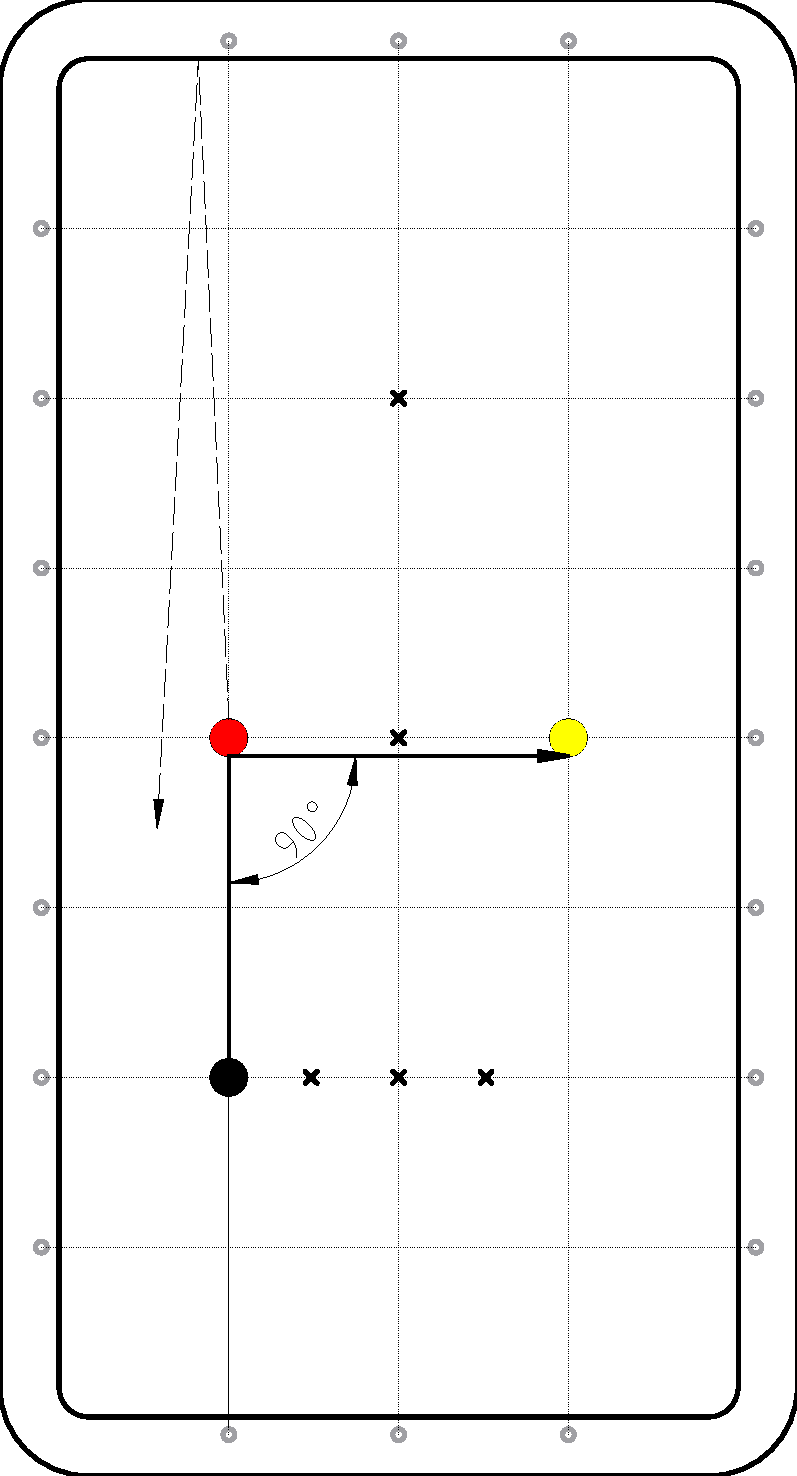
\includegraphics[width=0.85\linewidth]{A/imagesA/A08-1.pdf}
	\caption{Le 90�}
	\label{fig:a08-1}
\end{figure}
\clearpage

% !TeX spellcheck = fr_FR
% !TeX encoding = ISO-8859-1

\section{Bosse sur la bille colleuse}


Quoique ce point n'est g�n�ralement tent� que quand le 1bande est
difficile ou impossible, il constitue maintenant un bon exercice de
ma�trise qui nous servira et nous suivra m�me jusqu'en cinqui�me ann�e
o� il va contribuer � l'apprentissage du point dit � � l'Am�ricaine
\textgreater{}\textgreater{} car il donne le pouvoir de bien contr�ler
la 2 le long d'une bande.

La 2 collant la bande fait corps avec elle. Elle va nous servir de
rebond pour la 1. Comme la 1 rencontre une forme circulaire au point
d'impact (de m�me mesure qu'elle), l'angle de r�flexion sera le double
de l'angle d'incidence. Pour �valuer la grosseur de bille � � prendre �,
on peut appliquer la r�gle du r�tro (image de la 3 dans la rouge). On
peut aussi calculer cette prise en L 3 imaginant une petite construction
: Tracer mentalement une droite reliant les billes 1 et 2. Tracer une
perpendiculaire � cette droite passant par le centre de la 2. Consid�rer
la bille 3', image sym�trique de la 3 par rapport � la perpendiculaire
cit�e. Ne regardons plus maintenant la 3 mais la 1, la 2 et la 3'... Il
ne reste plus qu'� appliquer un simple coul�. Cette technique semble
tr�s compliqu�e sur le papier mais l'est beaucoup moins sur le tapis...
Elle donne cependant une l�g�re erreur mais insuffisante pour rater le
point tant que l'angle de r�flexion n'exc�de pas 45�.

Attention : jouer sans effet ! (fig. 1) Pr�caution : malgr� l'attention
qu'on y apporte, la 2 colle rarement la bande. Le moindre espace modifie
la donne. Il sera prudent d'appliquer une nuance plus pleine ou bien un
petit effet contraire. � essayer sur place !

Si on applique un effet quelconque, la trajectoire de la 1 peut s'en
trouver tr�s chang�e.

\begin{itemize}
	\item
	Effet � gauche : prendre la 2 un peu plus fine : celle-ci � avance �
	vers le jeu.
	\item
	Effet � droite : prendre la 2 un peu plus grosse : celle-ci se d�colle
	sans avancer.
	\item
	Prise de bille haute : la 2 reste � �cras�e � (coll�e) sur la bande.
	Le mouvement de la 1 est ralenti.
	\item
	Prise de bille basse : la 2 se d�colle. Le retour de la 1 est rapide.
	\item
	Figure 2 : c'est un angle droit. Appliquons un angle de 45�, celui de
	retour sera de 90�. A cause de � l'�crasement de la 2 sur sa bande, la
	pratique montrera qu'une prise un peu plus grosse que la demi-bille
	assure mieux...
	\item
	Dernier cas : si la 2 ne colle pas la bande : Ne visez plus l'image de
	la 3 dans la rouge mais bien un point plus proche du centre de la 2.
	Ce point devrait �tre calcul� en partant de ladite image et en entre
	la distance de la 2 � sa bande proche. Attention, si cette distance
	porte le point de vis�e au-del� du centre, le point-bosse n'est plus
	possible. Il faut choisir une autre solution.
\end{itemize}

\begin{figure}[htb]
	\centering
	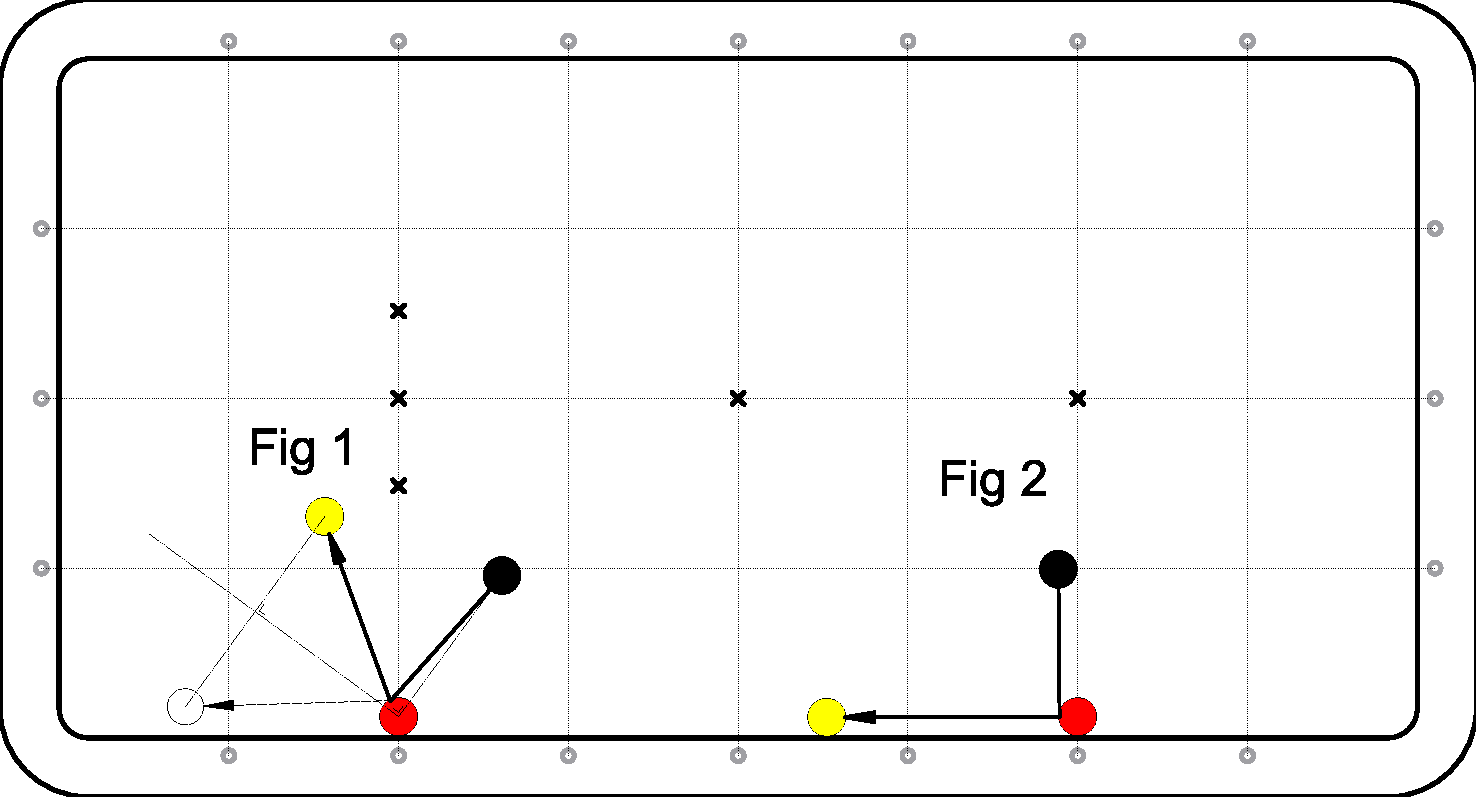
\includegraphics[width=\linewidth]{A/imagesA/A09-01.pdf}
	\caption{Bosse sur la bille colleuse.}
	\label{fig:a09-1}
\end{figure}
\clearpage

% !TeX spellcheck = fr_FR
% !TeX encoding = ISO-8859-1

\section{Le 1 Bande}

Le 1 bande est un point tr�s fr�quent. Nombreux sont ceux qui se
contentent d'ex�cuter ce point seulement pour ne pas perdre leur tour.
C'est l�, n�gliger la position �ventuellement � exploiter.

En th�orie, il suffit de toucher la 2 de mani�re � percuter la bande au
milieu du segment de bande obtenu en projetant l'image des billes 2 et 3
perpendiculairement sur lui, la 2 et la 3 d�terminant une parall�le �
ladite bande. Si la direction 2-3 n'est pas parall�le � la bande, il
faut s'imaginer le mouvement de � retour � de la 1 pour appliquer une
correction � la th�orie. Avec l'habitude, cette correction � sautera �
aux yeux. Contentons-nous, pour cette premi�re approche, de cas o� les
billes 2 et 3 sont sur une droite parall�le � la bande.

Fig.1 : La distance entre la 2 et la 3 est � peu pr�s le double de la
distance de ces billes � la bande. La th�orie s'applique. Prendre la 2
en demi-bille de mani�re � percuter la bande au milieu du segment comme
d�crit plus haut.

Fig.2 : La distance entre la 2 et la 3 est plus grande que le double de
la distance de ces billes � la bande. La 2 pourrait �tre prise fine mais
il est souvent pr�f�rable de la prendre un peu trop grosse de mani�re �
faire avancer la 2 vers la 3 et de corriger par un bon effet.

Fig.3 : La distance entre la 2 et la 3 est plus petite que le double de
la distance � la bande. En jouant la 2 grosse, on risque que celle-ci
percute la 3 avant l'arriv�e de la 1. Il conviendra de jouer trop fin et
d'apporter une correction par l'effet contraire.

Fig.4 : Cas particulier : la 1 est � bande, et la 2 � une distance
inf�rieure � une bille. Pour une prise en demi-bille jou�e parall�lement
� la bande, appliquons un bon effet pour un angle inf�rieur � 45�, pas
d'effet pour un angle de 45� et effet contraire pour un angle sup�rieur
� 45�. Le r�sultat, en douceur, est surprenant. Si la distance 2-bande
est inf�rieure � une demi-bille sans �tre � masquante �, on peut encore
passer mais prudence : le coup peut se faire masquer par la 2. Si la
distance 2-bande est sup�rieure � une demi-bille, l'effet contraire sera
plus souvent n�cessaire.

Remarque :

\begin{itemize}
	\item
	Le point de base sera rapidement assimil�. L'entra�nement conseill�
	est de s'acharner jusqu'� ce que � chaque r�alisation, les 3 billes
	soient dans un � chapeau �, assurant ainsi la suite de la s�rie...
\end{itemize}

\begin{figure}[htb]
	\centering
	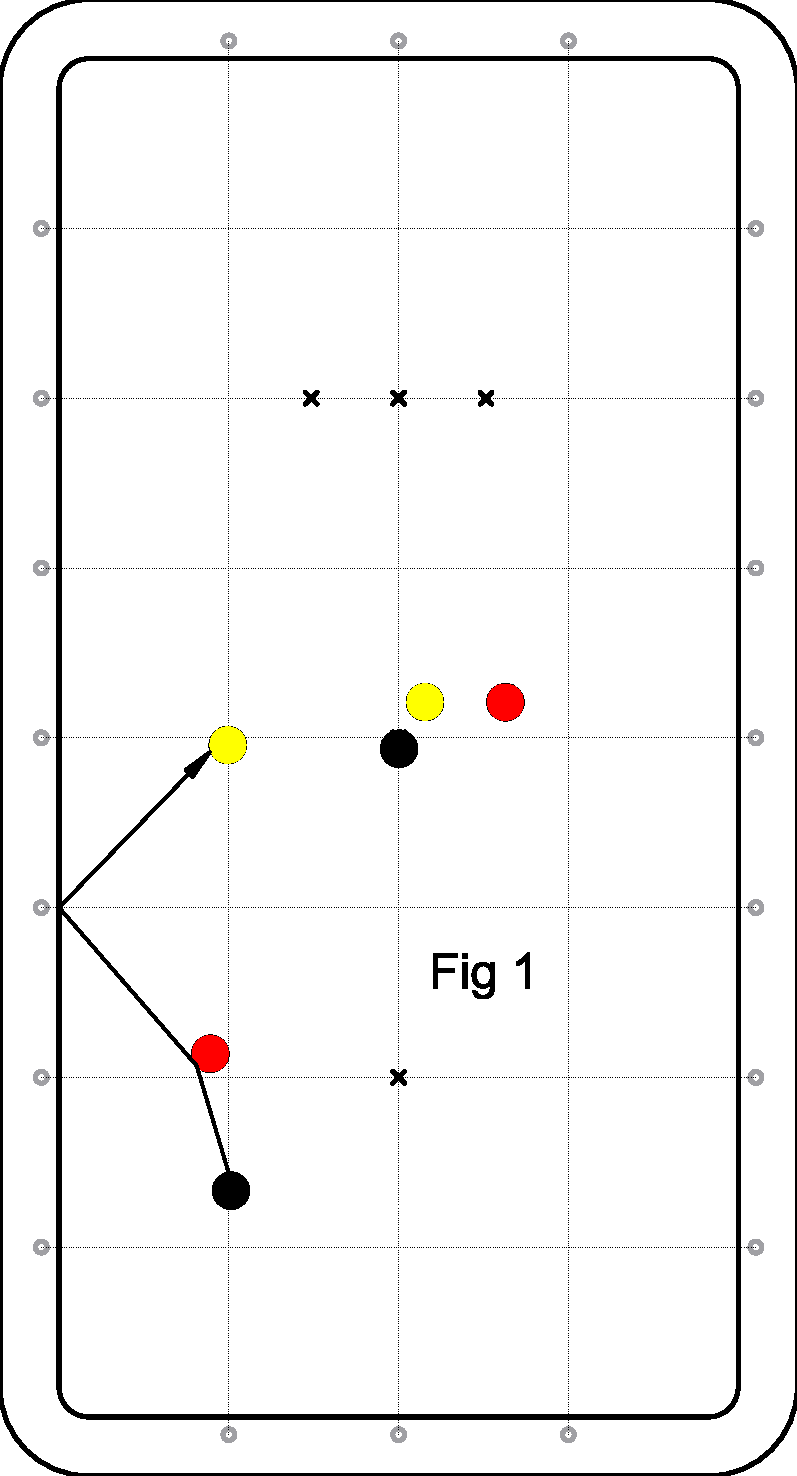
\includegraphics[width=0.85\linewidth]{A/imagesA/A10-01.pdf}
	\caption{Le 1 Bande}
	\label{fig:a10-1}
\end{figure}
\begin{figure}[htb]
	\centering
	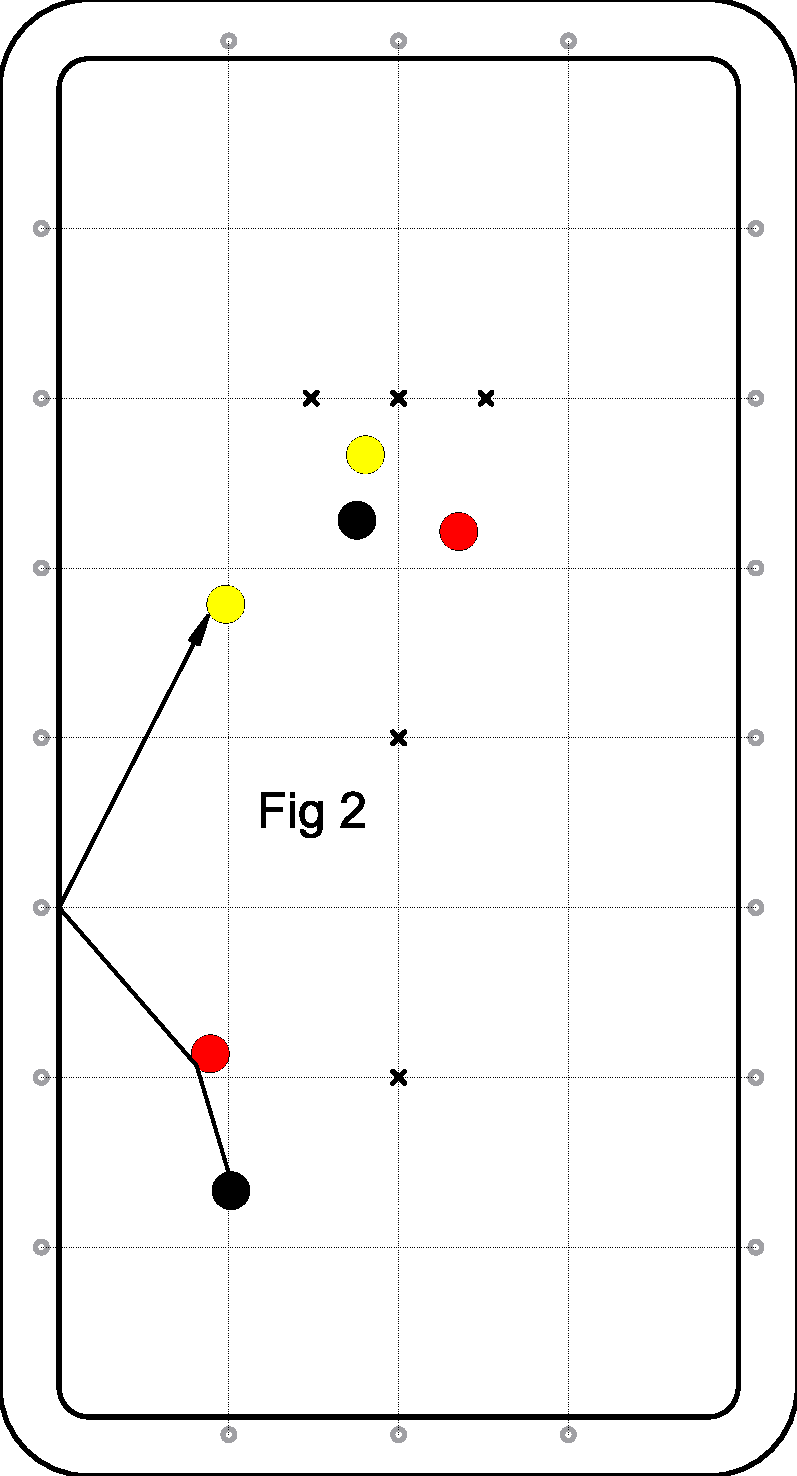
\includegraphics[width=0.85\linewidth]{A/imagesA/A10-02.pdf}
	\caption{Le 1 Bande}
	\label{fig:a10-2}
\end{figure}
\begin{figure}[htb]
	\centering
	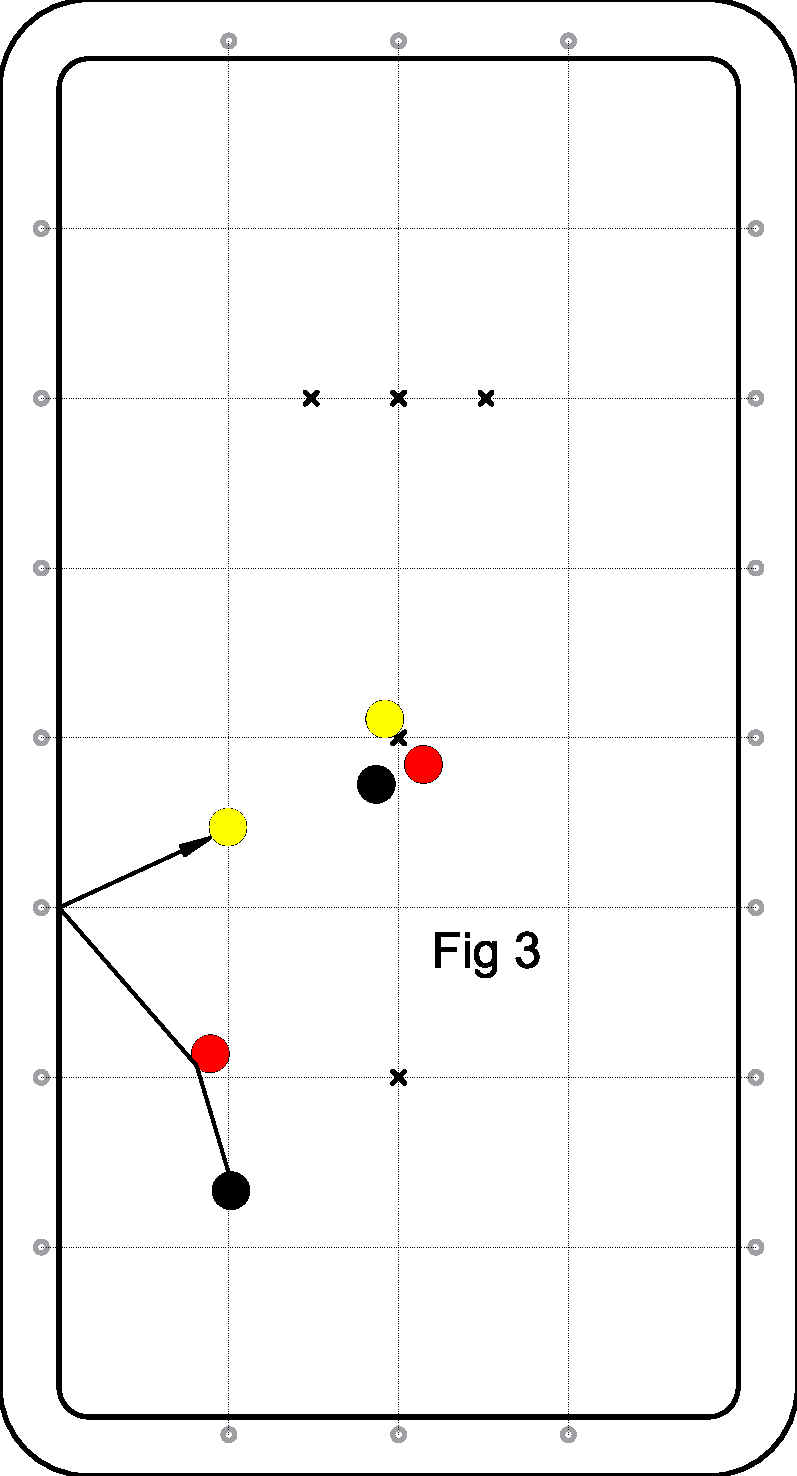
\includegraphics[width=0.85\linewidth]{A/imagesA/A10-03.pdf}
	\caption{Le 1 Bande}
	\label{fig:a10-3}
\end{figure}
\begin{figure}[htb]
	\centering
	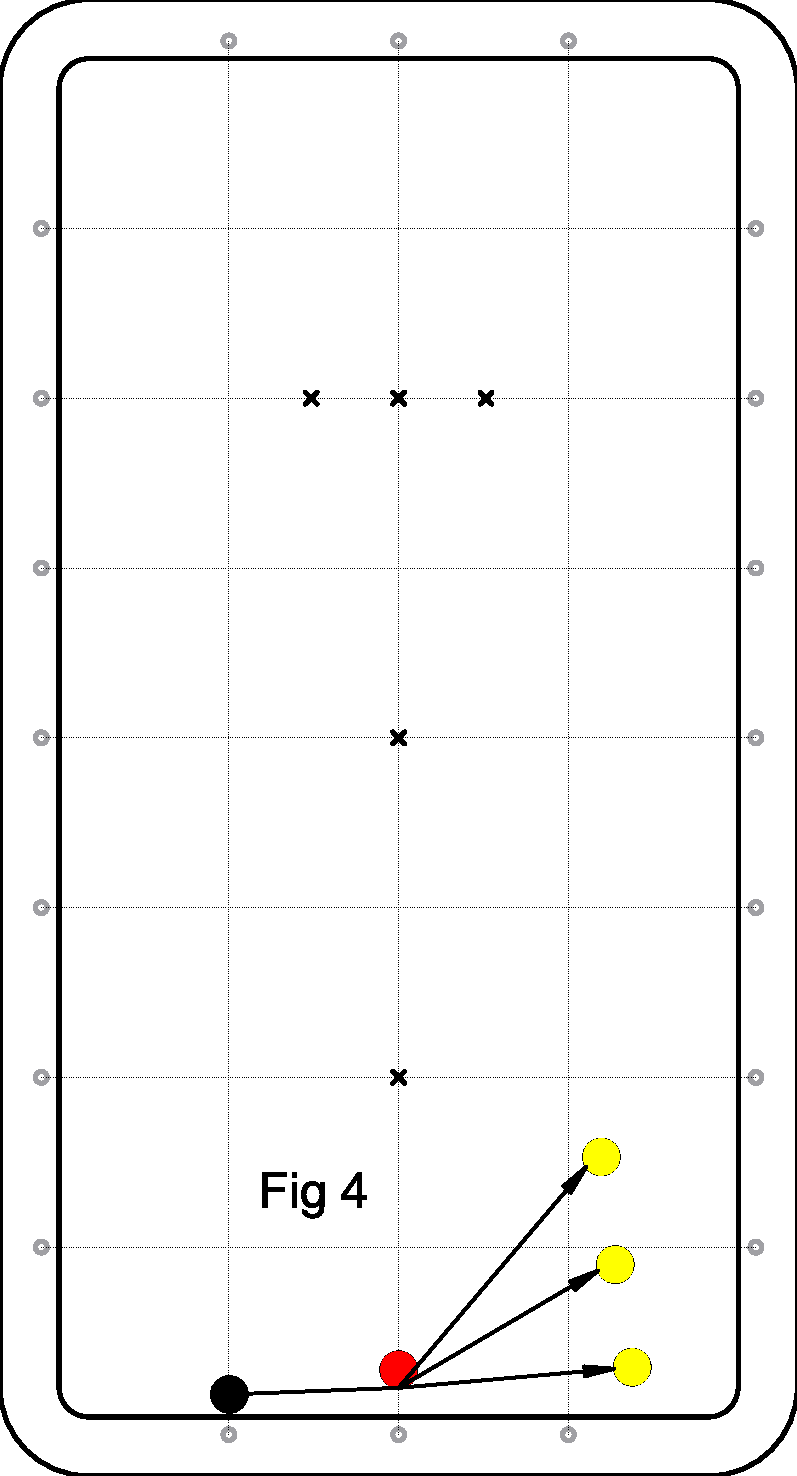
\includegraphics[width=0.85\linewidth]{A/imagesA/A10-04.pdf}
	\caption{Le 1 Bande}
	\label{fig:a10-4}
\end{figure}

\clearpage

% !TeX spellcheck = fr_FR
% !TeX encoding = ISO-8859-1

\section{2 bandes retour par la bissectrice}

La bissectrice de l'angle de coin offre la particularit� � d'attirer �
les billes en rendant leur mouvement parall�le � elle : ce n'est
�videmment pas vrai ! Il s'agit d'une tendance seulement et dans
certains cas, cette tendance nous sera bien utile. Si une bille roule
parall�lement � la bissectrice, mue d'un effet normal mais favorable,
elle reviendra parall�lement � cette bissectrice, sym�triquement au
premier mouvement (ou presque).

Figure 1 : Cette figure illustre cette particularit�. Bien que lorsque
nous aurons atteint un certain niveau nous n'y penserons plus, il est
int�ressant de s'exercer � ce point. Les billes 2 et 3 sont situ�es sur
des parall�les de chaque c�t� et �quidistantes de la bissectrice.
N'h�sitons pas ! Prenons la 2 de telle sorte que le trajet de la 1 soit
parall�le � la bissectrice et mue d'un effet favorable. La 1 revient par
le coin, parall�le et sym�trique � son premier trajet par rapport � la
bissectrice : le point, d'apparence d�licate, est devenu inratable !

Figure 2 : Ceci illustre seulement une tendance qu'il conviendra de se
rendre famili�re. La 3 est situ�e sur la bissectrice de l'angle de coin
et la 2 pr�s d'une bande (ici la petite mais le probl�me est valable sur
la grande aussi mais la position des billes est alors rarement aussi
int�ressante car la grande bande � �carte le jeu
\textgreater{}\textgreater{} et la petite � ram�ne �). Prendre la 2 en
visant le milieu de la portion de bande entre la 2 et le coin, effet
favorable, haut de bille. Je dis bien viser et pas toucher ! En effet,
vu la dimension de la bille, celle-ci touchera un peu avant le milieu si
le point est court (distance 2-coin courte) et assez bien avant, si le
point est long (distance 2-coin longue).

Remarque :

\begin{itemize}
	\item
	Ce point est plus � � sentir � qu'� calculer.
	\item
	Certains billards allongent et d'autres � cassent �. Il faudra en
	tenir compte.
	\item
	Un effet bas de bille � rabat �. Pour � soulever �, il faut viser la
	bande, plus pr�s de la 2 que du coin, pour rabattre, plus pr�s du
	coin.
	\item
	Attention, si la 2 est �cart�e de la petite bande de plus de dix
	centim�tres environ, il conviendra de viser plus pr�s du coin, etc.
\end{itemize}

Il existe donc beaucoup d'adaptations � ce point qui seront volontiers
propos�es lors de la pr�sentation � sur le terrain �.

\begin{figure}[htb]
	\centering
	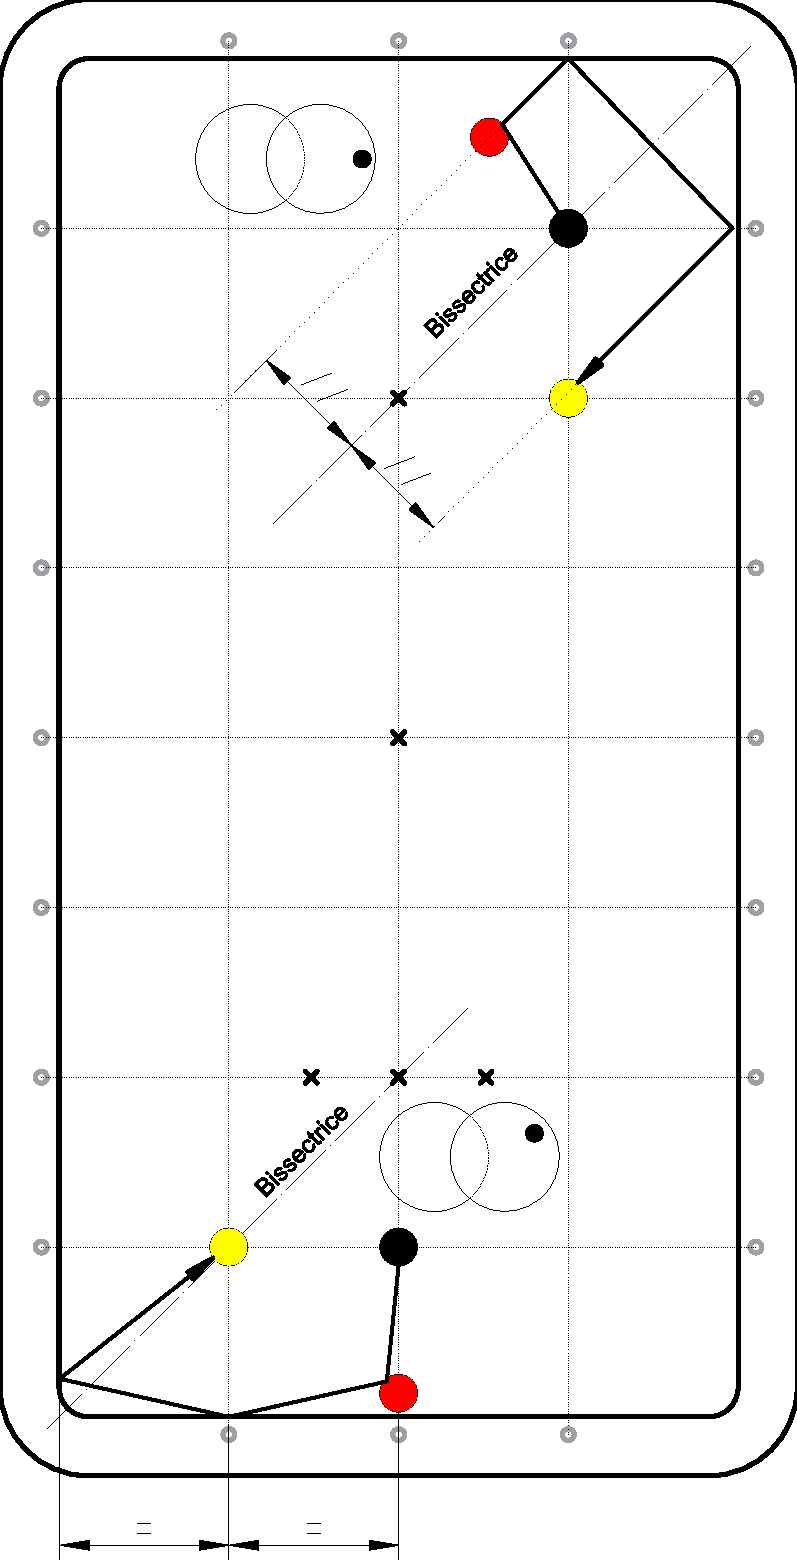
\includegraphics[width=0.85\linewidth]{A/imagesA/A11-01.pdf}
	\caption{2 bandes retour par la bissectrice.}
	\label{fig:a11-1}
\end{figure}
\clearpage

% !TeX spellcheck = fr_FR
% !TeX encoding = ISO-8859-1

\section{Le	coul�-bande}

Nous avons d�j� vu le coul� simple. Ici, une difficult� suppl�mentaire
appara�t : de par la disposition des billes, la 1 sera emp�ch�e par une
bosse avec la 2.

Figure 1 : Cette figure illustre le cas o� la 2, apr�s le choc d'avec la
1, percute la bande puis vient se mettre dans le chemin de la 2. Une
autre solution devra �tre trouv�e, si possible une finesse, un mass�
(voir 3�ann�e - les planches �C�), un 1 bande sur une autre bande ou
m�me carr�ment une carambole dans les cas les plus difficiles. Cette
solution alternative permet de rester au billard mais donne rarement une
position de \textless{}\textless{} construction �.

Figure 2 : On peut pallier l'inconv�nient du contre en coulant � droit
devant � avec un maximum d'effet contraire par rapport � la 2. Celle-ci,
imprim�e d'un effet contraire, s'�carte de la perpendiculaire � la bande
et �vite la 3 et surtout aussi, la 2 au retour comme l'indique le
pointill�. La 1, maintenant, a le champ libre et fonce sur la bande
droit devant mue d'un effet important (effet toupie), favorable � une
d�viation vers la 3. Les billes 1 et 2 ont donc un mouvement de
d�solidarisation. La 1 reste en position dominante, face aux billes 2 et
3, chass�es du m�me c�t�. Port� moyennement fort, le coup donne
suffisamment d'�nergie pour permettre � la 2 de revenir dans le jeu par
doublage. Ce point demande une bonne pr�cision mais si on joue
absolument droit c�d absolument plein sur la 2 avec le � plein
\textgreater{} effet, la r�ussite est certaine !

Figure 3: Vu la situation, on aurait pu tenter un direct mod�r� ce qui
pourrait donner au coup suivant, un r�tro � rentrant � les billes dans
le � tiers �. Cependant, si on se sent bien,
appliquant un � coul�-bande � comme pour la figure 2, le coup est sans
danger et chasse imm�diatement les billes dans le tiers. Cette solution
donne souvent plus de chance de � serrage � du jeu.

Remarque : si on parvient � couler en � descendant � dans la 1, l'effet
imprim� sera tr�s important et nous permettra de r�aliser des angles
tr�s � �tal�s � au rebond, voire, comme on dit parfois, faire des angles
� impossibles �. Acharnons-nous : la droiture du corps et la position
ferme de la main doivent �tre parfaites...

\begin{figure}[htb]
	\centering
	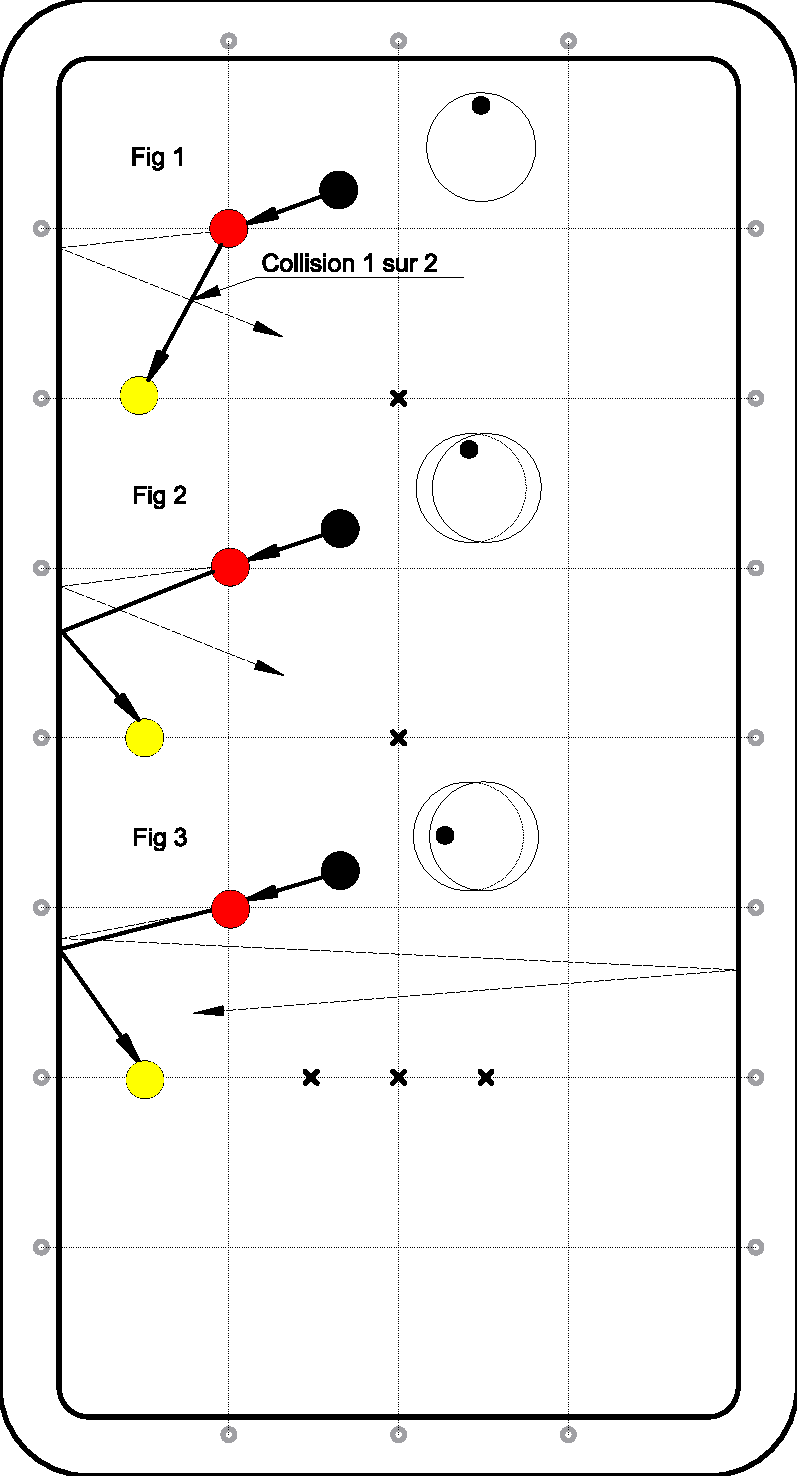
\includegraphics[width=0.85\linewidth]{A/imagesA/A12-01.pdf}
	\caption{}
	\label{fig:a12-1}
\end{figure}
\clearpage

% !TeX spellcheck = fr_FR
% !TeX encoding = ISO-8859-1

\section{Le coul�-bosse}

Le coul� simple est ais�ment appris, m�me par un d�butant. Le coul�
bande est un peu plus difficile. Le coul� bosse l'est encore davantage.
La � bosse � fait peur. Une fois cette peur vaincue, le point devient
plus facile. Encore une fois, la confiance en soi travaille pour la
r�alisation du point.

Figure 1 : La 2 colle la bande. Viser une moiti� de bille du r�tro (pour
un angle inf�rieur au droit), prise en t�te (haut de bille) et avec
effet contraire maximum. Faisant corps au moment du choc, les billes 1
et 2 se d�tachent ensemble pour venir en jeu serr� � la 3. Une
possibilit� de s�rie s'annonce...

Figure 2 : La 2 ne colle pas. La prise de la 2 est la m�me que celle
pour la figure 1 mais peut-�tre un peu plus grosse, comme si on jouait
pour effleurer l'int�rieur de la 3. La bosse de la 2 en retour sur la 1
repousse celle-ci vers l'ext�rieur de la 3. Ici encore, le jeu se serre
et annonce une s�rie possible...

Figure 3 : On peut r�aliser ce point avec ou sans bosse. Avec bosse,
appliquer un effet inverse au sens du jeu. Le coul� est direct en visant
comme si la 3 se trouvant � devant � elle-m�me. La bosse de la 2 au
retour de la bande sur la 3, pousse la 3 sur la 1, �ventuellement pour
la seconde fois si la 1 avait d�j� percut� la 3. On esp�re que la bosse
de la 3 sur la 1, permet � l'axe 2-3 de ne pas se masquer � la 1 sinon :
c'est la ligne droite : une hantise pour les amateurs de billard. Sans
bosse : mettre l'effet dans le sens du jeu. Cette prise exige une plus
grande pr�cision dans la force � appliquer : la 2 ne rencontrant plus le
barrage au retour, risque de s'�carter loin du jeu ou de rester en de��
et d'offrir encore une fois, trois billes align�es. L'id�al serait que
la 2 vienne � hauteur de la 3 ou s'�carte l�g�rement. En tous cas, il ne
faut pas tenter ce coup pour subir une bosse non d�sir�e, le r�sultat
serait impr�visible.

Figure 4 : C'est une variante de la figure pr�c�dente. Nous ne sommes
plus face � la bande mais bien au coin. La 2 revient par deux bandes
avec des trajectoires parall�les � l'axe. L'effet doit toujours �tre
favorable et la bosse arri�re presque toujours �vit�e.


\begin{figure}[htb]
	\centering
	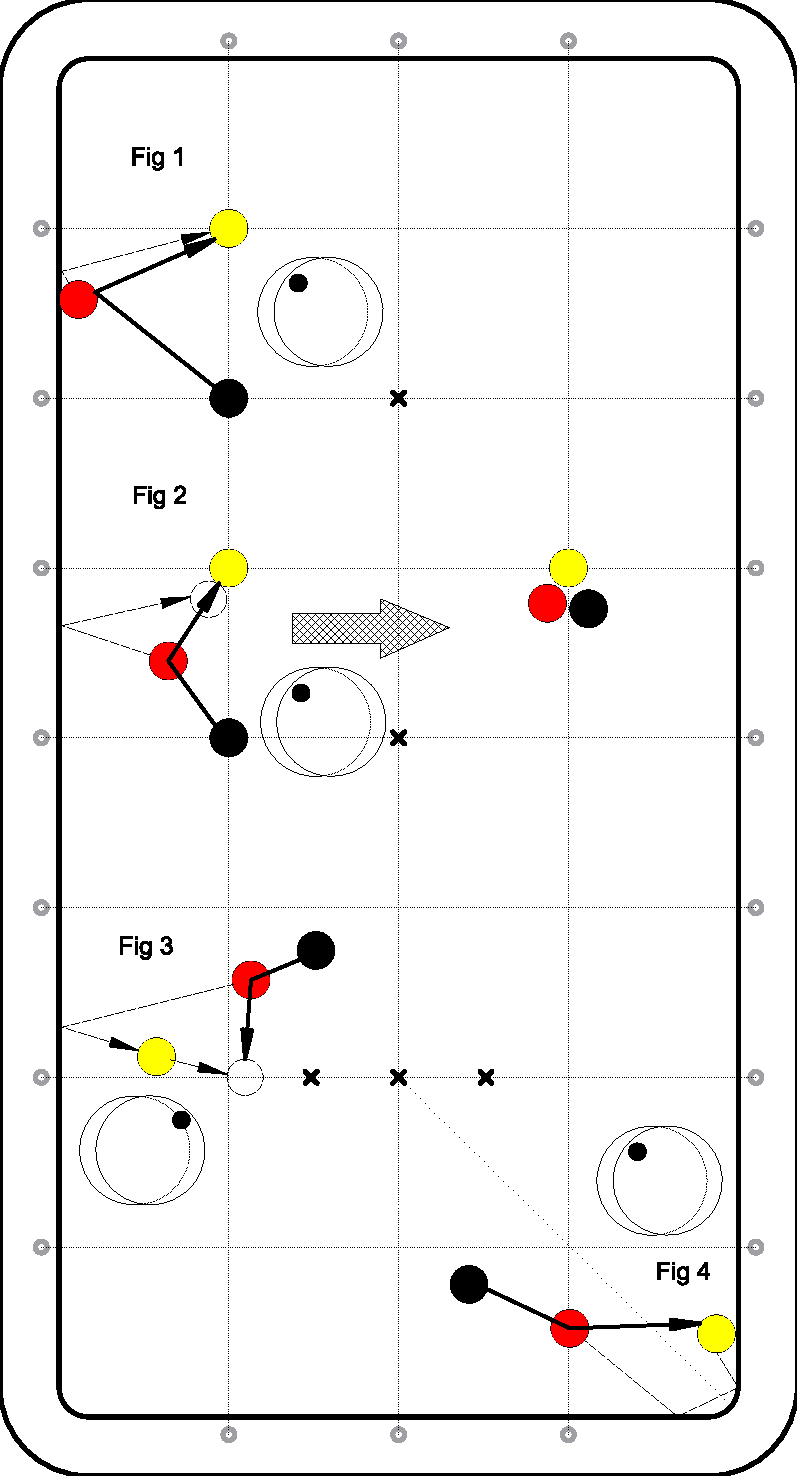
\includegraphics[width=0.85\linewidth]{A/imagesA/A13-01.pdf}
	\caption{Le coul�-bosse}
	\label{fig:a13-1}
\end{figure}
\clearpage

% !TeX spellcheck = fr_FR
% !TeX encoding = ISO-8859-1

\section{Le r�tro-bande}

Une fois la technique du r�tro bien en main, on s'habituera facilement �
ce coup. Le ramen� ou rappel est plus ou moins s�r. Cependant, l� o� le
r�tro direct ne ram�ne pas directement, il est parfois possible de
s'assurer une rentr�e convenable en s'aidant de la bande, se figurant
une bille 3 virtuelle plac�e de l'autre c�t� de la bande qui lui est
proche sym�triquement � la 3 r�elle (donc en dehors de la table). En
voici deux exemples :

Figure 1 : Le r�tro direct est une solution mais il entra�ne la 2 hors
de la rentr�e. La 2 toucherait la petite bande trop loin du coin oppos�
et elle s'�carterait irr�m�diablement. Pour minimiser cet �cart :
prendre la 2 en r�tro de pr�f�rence basse, effet droit si la direction
1-2 est loin du coin et effet gauche si la direction 1-2 est trop pr�s
du coin et jouez comme si la 3 �tait situ�e sym�triquement de l'autre
c�t� de la bande qui lui est proche (3'). Id�alement, la 2 tournera via
la petite bande sup�rieure, la grande bande oppos�e, la petite bande
inf�rieure, la grande bande proche et vient s'arr�ter dans le barrage
form� par la 1 et la 3.

Figure 2 : Ce point est tout en d�licatesse. Un r�tro simple ferait
d'abord toucher la petite bande � la 2 qui ne pourrait plus rentrer. Si
la direction 1-2 coupe la petite bande mais tr�s � haut �, on peut
encore jouer r�tro direct avec effet ras du tapis maximum et contraire :
la 2 ne s'�cartera pas ou peu. Si la direction 1-2 coupe trop bas ou
bien trop haut sur la grande bande (� appr�cier), il est encore possible
de serrer le jeu en appliquant un r�tro bande effet contraire maximum.
En restant pr�s de la 3, la 1 constitue un barrage au retour de la 2.

Remarque : Ces deux exemples montrent des applications assez simples du
r�tro. Cependant, il ne faut pas s'y tromper et restons prudents. Ils
demandent un s�rieux entra�nement avant d'�tre poss�d�s, non seulement
pour la pr�cision du coup mais aussi et surtout pour la force n�cessaire

\begin{figure}[htb]
	\centering
	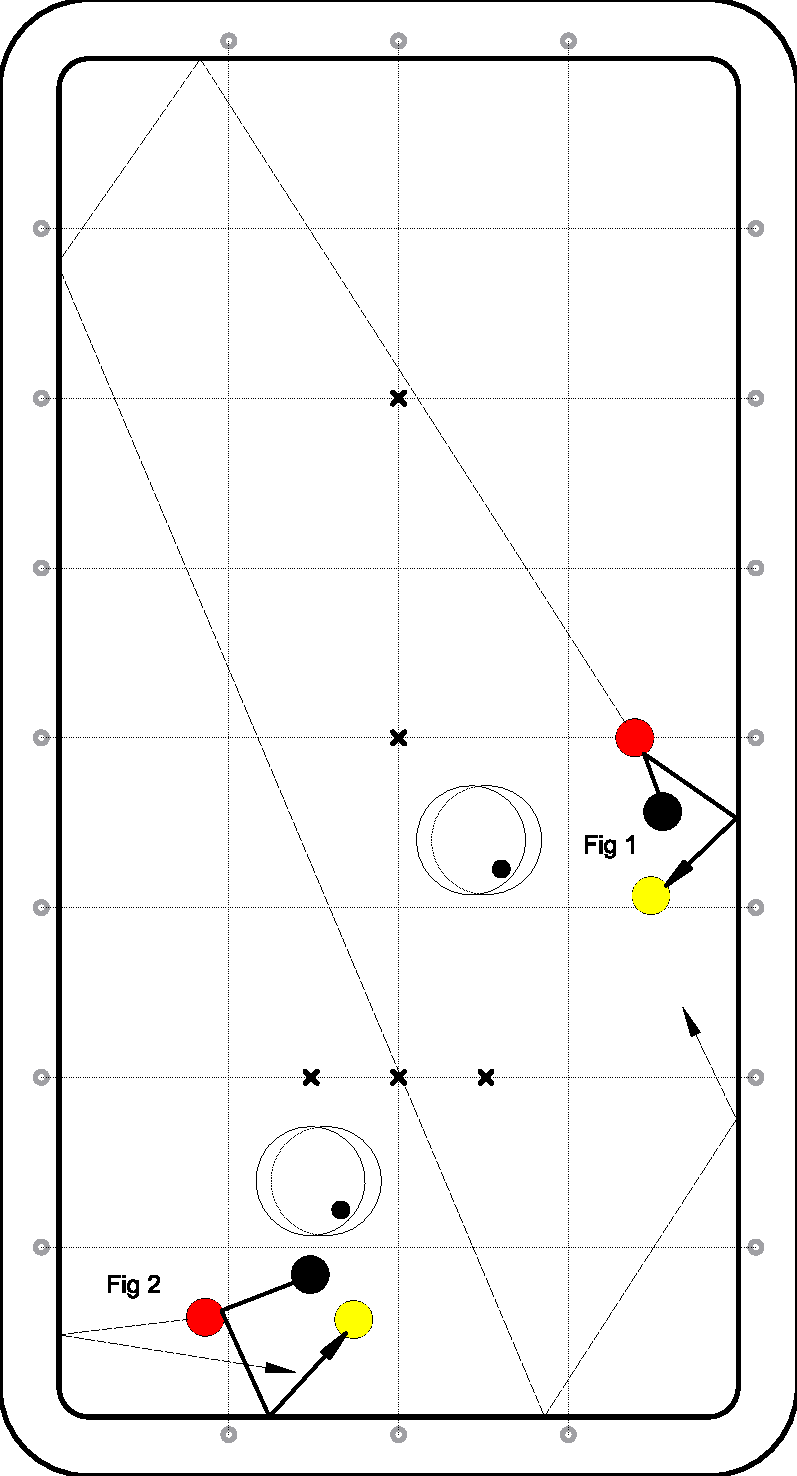
\includegraphics[width=0.85\linewidth]{A/imagesA/A14-01.pdf}
	\caption{Le r�tro-bande}
	\label{fig:a14-1}
\end{figure}
\clearpage

% !TeX spellcheck = fr_FR
% !TeX encoding = ISO-8859-1

\section{Le petit coul�}

Sans trop de danger, le petit coul� est possible jusqu'� une distance de
1 centim�tre entre les billes 1 et 2. Il demande une grande souplesse,
de la prudence et de la d�licatesse. A une distance plus courte, le
queut� est dangereux, c�d que la canne, selon la th�orie, serait encore
en contact de la 1 lorsque cette derni�re percuterait la 2 ce qui
constitue la d�finition officielle du queut�.

Bien que cette th�orie soit exacte, en pratique, la v�rit� est souvent
diff�rente. En fait, pour ex�cuter un coul�, il faut allonger, c�d
accompagner la 1 dans son mouvement. Fort bien, mais accompagner ne
signifie pas rester en contact sinon le proc�d� a frott�, la bille a
roul� en se frottant : c'est une faute qui est visible lorsque la fl�che
� roule � sur la bille. En r�alit�, le proc�d� reste en contact tr�s peu
de temps. La 1 subit une acc�l�ration qui la d�tache directement du
proc�d� mais subit un ralentissement au choc avec la 2 avant d'acc�l�rer
� nouveau sous l'impulsion de l'effet longitudinal produit par
l'accompagnement de la canne. C'est ce ralentissement qui fait danger
car la canne dans son mouvement avance encore... et risque de rattraper
la 2 � ce moment : queut� ! Ce queut� est facile � d�pister pour
l'arbitre car les billes 2 et 3 auront tendance � se mouvoir en m�me
temps et � la m�me vitesse. Les � anciens \textgreater{}\textgreater{}
appellent cette faute : � une charrette �. L'arbitre, bien plac� sur le
c�t� de la direction des billes doit annoncer � faute � et passer la
main � l'autre joueur.

Le point se joue comme un coul� traditionnel, canne horizontale,
mouvement l�ger et prolongeant en veillant � retenir la canne avant que
la 1 ne percute la 2. Si la distance est vraiment trop courte, on peut
relever l�g�rement la fl�che d�s le coup port�. Cela rassure sur la
validit� du point mais plus tard, il sera pr�f�rable de ne pas le faire
pour une meilleure ma�trise du jeu serr�. Ce point fait peur. Beaucoup
lui pr�f�re un mass�.

Comme entra�nement, je conseillerais de placer les billes 1 et 2 � 5 cm.
l'une de l'autre et de r�aliser le coul� en rassemblant les 3 billes
dans un � chapeau � (les 3 billes doivent pouvoir �tre couverte par une
main ouverte). Ex�cuter des s�ries de 10 essais jusqu'� une s�rie
r�alis�e � 100\% de r�ussite (!). Ensuite placer les billes 1 et 2 � une
distance de 4 cm. Recommencer les s�ries. Puis placer les billes � 3 cm.
2 et enfin 1 cm.

C'est fastidieux... mais ce sera payant. Il conviendra de s'armer de
patience et d'obstination. Il faut prendre le temps n�cessaire de bien
poss�der cette �tape.

\begin{figure}[htb]
	\centering
	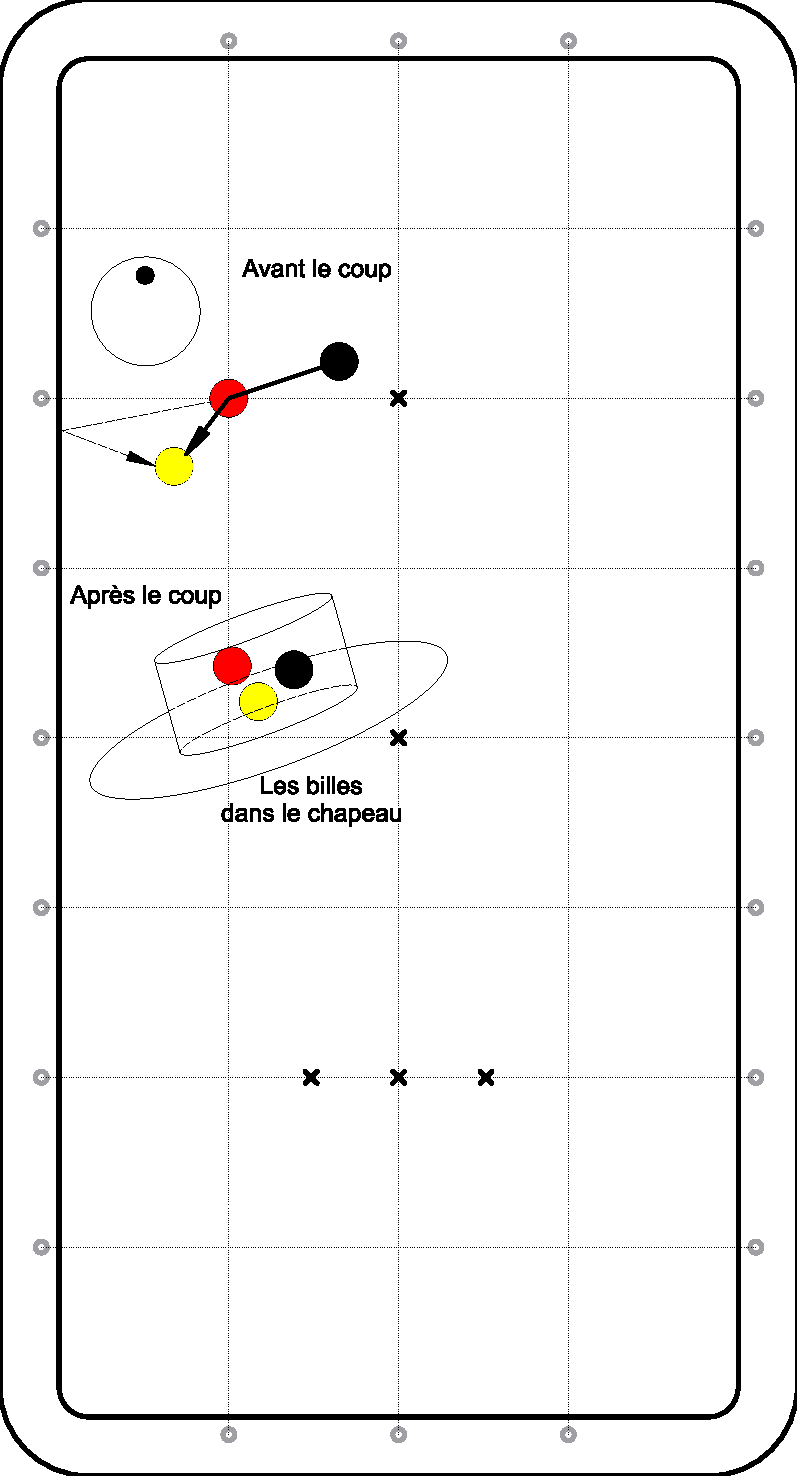
\includegraphics[width=0.85\linewidth]{A/imagesA/A15-01.pdf}
	\caption{Le petit coul�}
	\label{fig:a15-1}
\end{figure}
\clearpage

% !TeX spellcheck = fr_FR
% !TeX encoding = ISO-8859-1

\section{Le petit r�tro}

Le petit r�tro est un point d'une d�licatesse et d'une souplesse de
toute premi�re importance pour la construction des s�ries. Plus tard,
par la justesse du coup, il permettra de bien ma�triser le retour de la
2 � dans le paquet � et le maintien du � serrage �. Il est surtout �
employer lorsque les billes sont proches l'une de l'autre.

Les billes sont � ce point rapproch�es qu'on pourrait jouer fin ou gros,
le point est inratable. Il serait r�ussi mais pas pour autant, bien
choisi. En effet, du choix d�pendra la suite de la s�rie. La position de
la 2 est � soigner particuli�rement.

Figure 1 : pour l'entra�nement, nous placerons les billes 1 et 2 �
environ 5 cm. l'une de l'autre. Nous ex�cuterons le r�tro de mani�re que
la 2 revienne dans le � chapeau �. Quand nous aurons r�ussi 10 fois de
suite, placer les billes 1 et 2 � 4 cm. d'intervalle. Recommencez la
m�me s�rie d'essais puis placez les billes 1 et 2 � 3, � 2 et enfin � 1
cm d'�cart. Pour cet exercice, la main arri�re doit se rapprocher du
point de d�s�quilibre de la canne sans la presser. Nous veillerons �
appliquer �ventuellement un effet pour assurer le retour de la 2 dans le
paquet. Une fois cet �puisant exercice r�ussi � 100 \% (!), passez � la
figure 2.

Figure 2 : Les billes sont proches de la bande, la 2 en �tant la plus
proche. Appliquez le r�sultat de votre pr�c�dent exercice et veillez �
ce que la 2 revienne en percutant doucement la 1 qui fait barrage : sans
le savoir, vous venez d�j� de toucher aux pr�mices de la s�rie dite � �
l'Am�ricaine �.

Pour affiner votre coup, prendre la 2 la plus grosse possible tout en
veillant � la r�alisation du point, appliquer l'effet qui assure le
retour de la 2 vers la 1 en barrage (bon effet si la 2 est trop avanc�e,
contraire si la 2 est en retard). La main arri�re doit �tre rapproch�e
jusqu'au point de rupture de l'�quilibre de la canne. Ne pas jouer fort
mais souplement.

Remarque : ce point para�t facile. Qu'on ne s'y trompe pas, il ne l'est
pas. De sa bonne ex�cution d�pend la s�rie. Il est vraiment une des
bases de la s�rie am�ricaine, grande ennemie du manque de souplesse.
Attention ! On perd souvent la position pour avoir jou� trop fin !

\begin{figure}[htb]
	\centering
	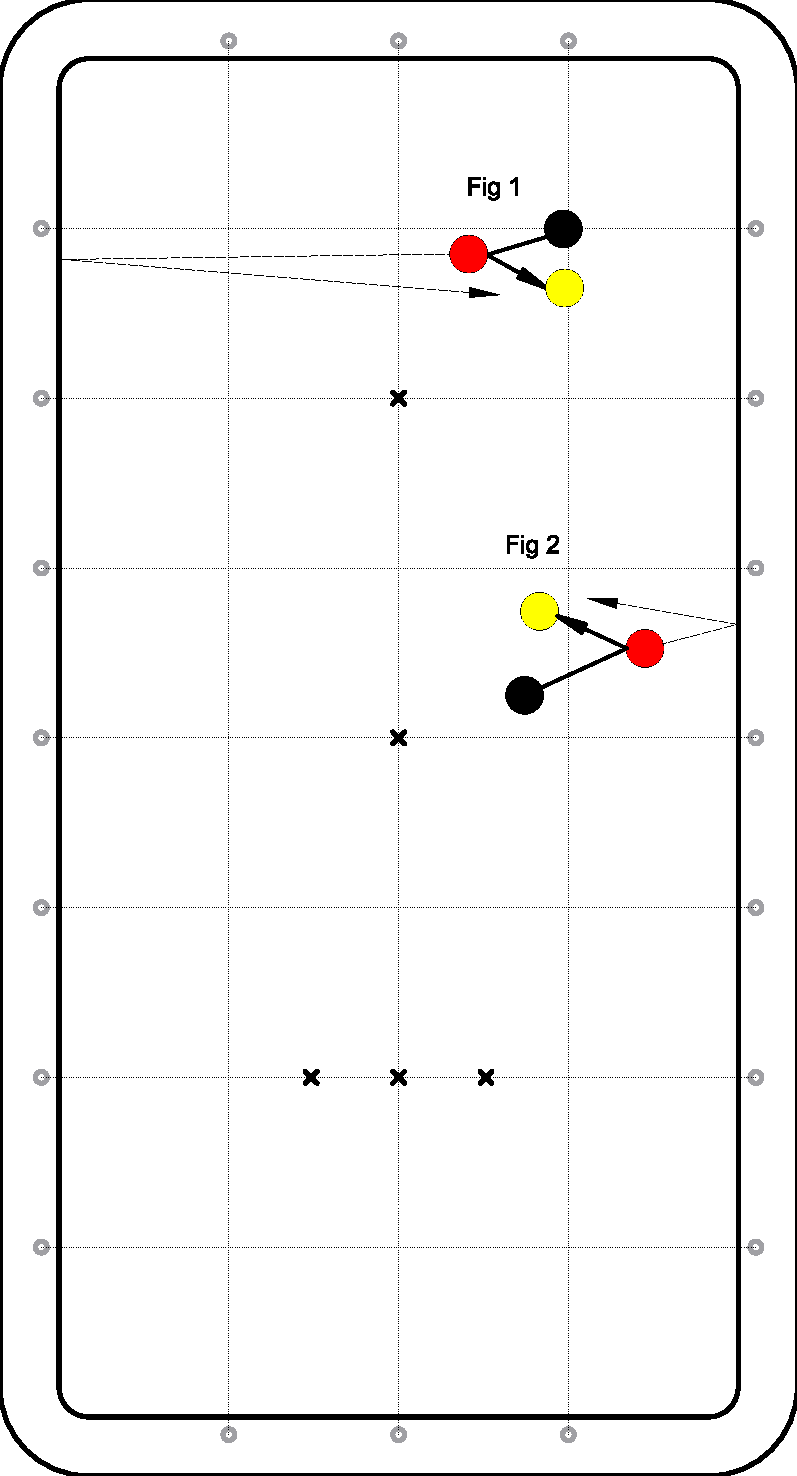
\includegraphics[width=0.85\linewidth]{A/imagesA/A16-01.pdf}
	\caption{Le petit r�tro}
	\label{fig:a16-1}
\end{figure}
\clearpage

% !TeX spellcheck = fr_FR
% !TeX encoding = ISO-8859-1

\section{Le trois bandes naturel}

Le 3 bandes naturel est ais� de conception et ram�ne le jeu dans le
coin. Les � vrais � joueurs de 3 bandes vous expliqueront qu'il faut
calculer les � mouches � (points de partage dessin�s sur les bandes de
la table) et jouer pr�cis�ment sur celles-ci si on veut faire le point.
Attention, ici nous parlons du jeu de libre ! Si le calcul des �
troisbandistes � (joueurs sp�cialis�s au jeu de 3 bandes) est exact, il
ne nous int�resse ici que tr�s secondairement et de toute fa�on, il est
beaucoup trop t�t pour s'y int�resser. Nous allons tenter de r�aliser en
ramenant la 2 dans le coin. Il y aura un risque de contre, cons�quence
de ce ramen�.

Comme pr�sent� sur la figure, on prend la 2 en demi-bille, coup prolong�
mais pas trop fort, l�ger effet favorable sur la premi�re bande. La
force du coup doit assurer le chemin, sans plus ! Parfois, on peut
affiner le point par une prise un peu plus grosse, de mani�re �
entra�ner la 2 � la suite de la 1, quitte � corriger la trajectoire de
la 1 par un effet un peu plus soutenu. Variante : prendre la 2 par la
gauche en deux tiers coul�s, effet haut �ventuel � gauche. Attention,
cette m�thode est souvent mal appliqu�e ; la 2 prise trop fine, reste en
� chemin �. D'une mani�re g�n�rale mais non exclusive, si la 1 est plus
proche ou �galement proche de la bande voisine que la 2, on pr�f�rera
tenter le 3B (3 bandes) dit naturel. Si la 1 est � �gale distance ou
bien plus �loign�e de la bande proche que la 2, on choisira de
pr�f�rence le 2B par l'avant (ici par la gauche).

Remarque : le contre de la 2 sur la 1 guette. Il suffira de jouer un peu
plus gros avec effet compensatoire ou bien un peu coul� pour l'�viter.

Entra�nement : placer les billes comme sur la figure, la 1 en face de la
troisi�me mouche en comptant � partir du coin sup�rieur (la partie
sup�rieure de la table est la partie la plus �loign�e du joueur lui-m�me
plac� sur un petit c�t�. Selon la position du joueur, le haut et le bas
de la table s'inversent). Placer la 1 en face de la premi�re mouche, �
partir du bas. La 3 est dans le coin. La 1 et la 2 � 30 cm. de la grande
bande. Ex�cuter donc ce point avec un taux de r�ussite d'au moins 70\%
la 2. Ensuite, faites varier la position de la 2, face aux trois mouches
sup�rieures, hormis le coin, puis faites varier la position de la 1 en
la pla�ant � 25cm. ou � 35 cm. de la grande bande.

En avant pour des s�ries d'essais ! Fameux entra�nement que celui-l�.
C'est tr�s fatigant... et amusant car les billes \textless{}\textless{}
voyagent �.


\begin{figure}[htb]
	\centering
	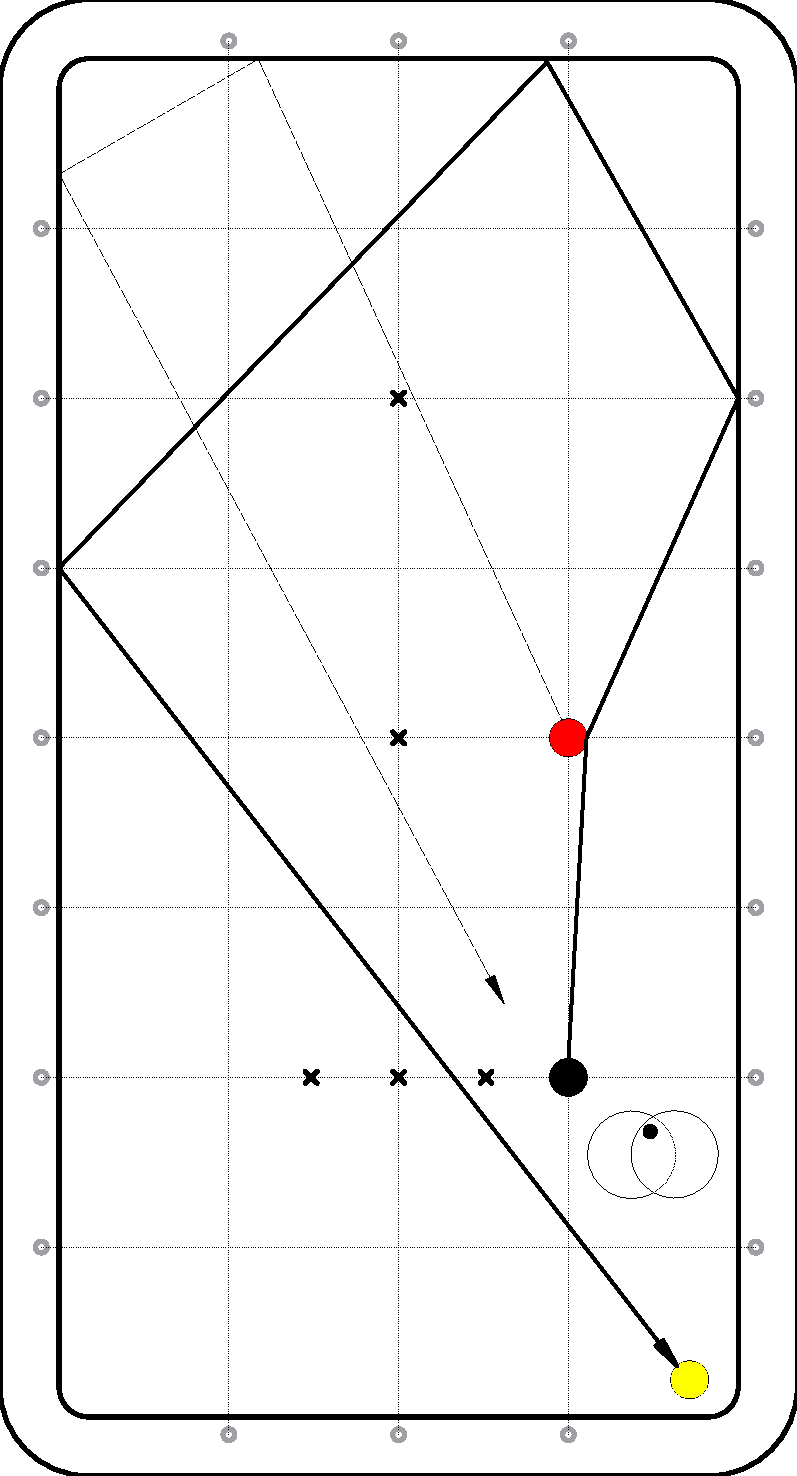
\includegraphics[width=0.85\linewidth]{A/imagesA/A17-01.pdf}
	\caption{Le trois bandes naturel}
	\label{fig:a17-1}
\end{figure}
\clearpage

% !TeX spellcheck = fr_FR
% !TeX encoding = ISO-8859-1

\section{R�tro Bille-Bande naturel}

Cette position est tr�s fr�quente. Elle permet souvent de ramener la 2
dans � le tiers � et m�me dans le � chapeau �.

Figure : imaginons une bille virtuelle 3' plac�e � l'ext�rieur de la
table sym�triquement oppos�e � son homologue, la bille 3 par rapport �
la grande bande proche. Ne pensons plus � la 3. Consid�rons maintenant
les billes 1, 2 et 3'. Appliquons un r�tro direct. La 1 est jou�e basse
mais pas trop, de mani�re � donner une bonne �nergie � la 2 qui doit
faire le tour de la table alors que la 1 doit s'arr�ter � la 3! On peut
mettre un effet � gauche pour assurer le retour de la 1. La bande coupe
le retour de la 1 pour la d�vier de sa trajectoire de la 3' vers la 3.
L'effet, plus ou moins appliqu�, peut obliger � viser plut�t le dessus
de la 3'. L'application de l'effet bon ou contraire sera fonction de
l'angle 1-2 / grande bande. La principale difficult� sera la force de la
frappe permettant de ramener la 2 dans, un chapeau, aux environs de la
3.

L'angle 1-2 / grande bande doit �tre appr�ci� avant l'essai. Quelques
exemples : a - L'angle en question pr�sent� sur la figure est id�al.
Prise basse en trois quarts, peut-�tre un l�ger effet favorable. Le coup
est moyen et de force moyenne. Cette position est la plus favorable. Ce
n'est pas toujours le cas.

b- L'angle est assez faible (moins de 309). Appliquez un r�tro direct.
La 2 revient en 3 bandes ou 4.

c - L'angle est encore plus petit (10o...). Appliquez un r�tro bande,
effet contraire. La 2 revient en une bande voire deux en s'�cartant un
peu de la grande bande mais pas trop.

d - L'angle est encore plus petit, voire presque nul. Ce sera � voir sur
place. Selon le cas, on appliquera le c - ou bien un r�tro direct,
toujours effet contraire qui permettra � la 2 de peu s'�loigner de la
grande bande au retour.

e - Cas sp�cial : l'angle est trop grand, trop large... et apparemment
ne permet plus de faire tourner la 2. Attention � bien interpr�ter ce
cas sp�cial. La 2 va toucher la grande bande oppos�e avant la petite
bande sup�rieure, nous le � sentons �.

Deux solutions :

\begin{itemize}
	\item
	Appliquer un r�tro direct sur la 3. Le jeu n'est plus ramen� mais les
	billes sont devant nous et permettent d'envisager � nouveau une
	construction de l'autre c�t� de la table.
	\item
	Tentons le diable en appliquant un r�tro bande comme dans le cas
	g�n�ral mais assez haut sur la 1, en dessous du milieu de la bille
	parce qu'il s'agit d'un r�tro et assez haut pour emp�cher une trop
	grande vitesse de la 1 au retour. La 2 est percut�e assez violemment,
	prend le coin sup�rieur en effet contraire et revient dans le chapeau
	! (Pas facile)
\end{itemize}

Entra�nement :

\begin{itemize}
	\item
	Tenter chaque cas des exemples : 100 \% pour le cas g�n�ral, 90\% pour
	les autres.
	\item
	L'exemple e : regardons-le comme un cas singulier mais tout de m�me :
	essayons...
\end{itemize}

\begin{figure}[htb]
	\centering
	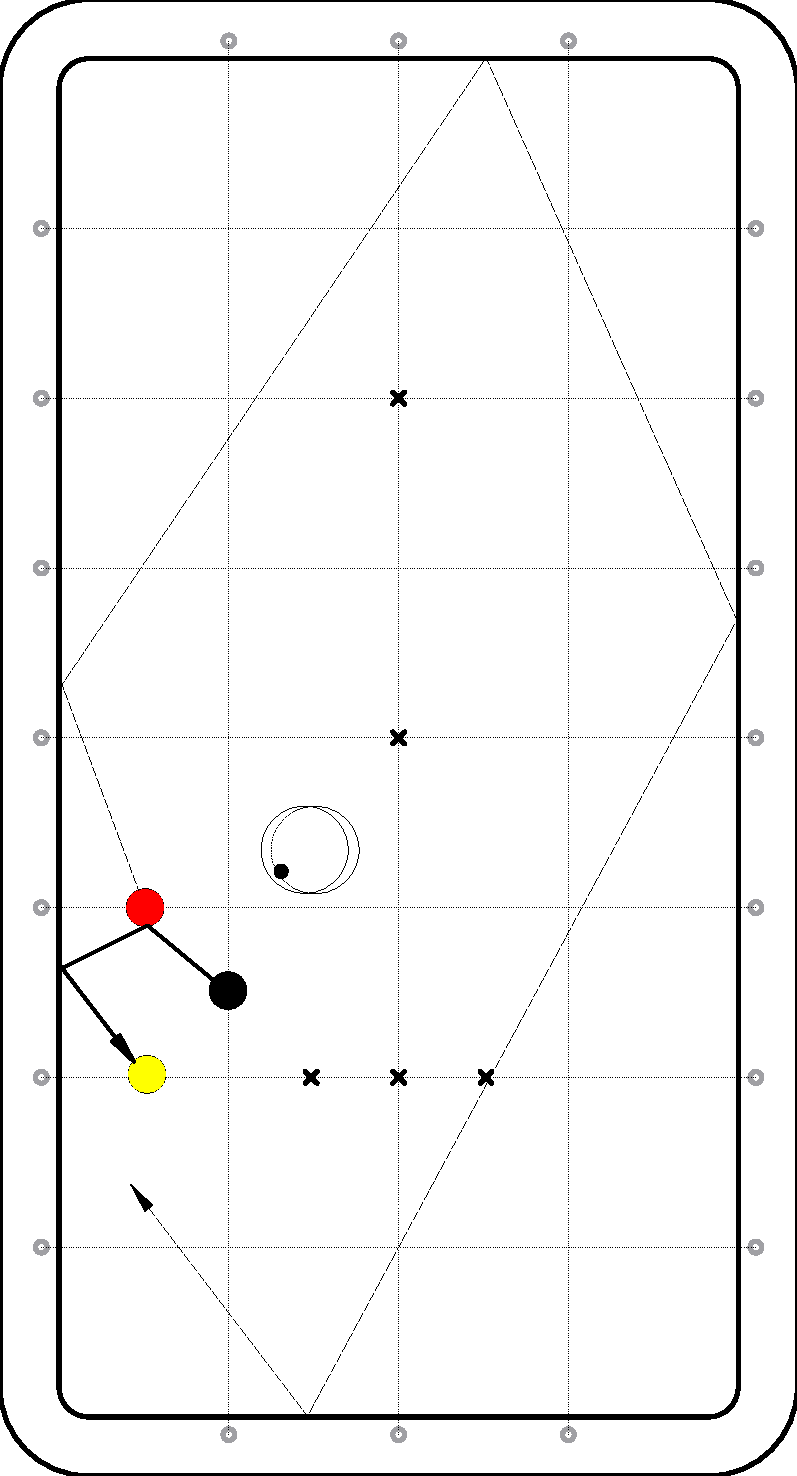
\includegraphics[width=0.85\linewidth]{A/imagesA/A18-01.pdf}
	\caption{R�tro Bille-Bande naturel}
	\label{fig:a18-1}
\end{figure}
\clearpage

% !TeX spellcheck = fr_FR
% !TeX encoding = ISO-8859-1

\section{Le Carrousel}

Le carrousel est un point assez facile. Il est aussi appel� le �
tourniquet �. La principale difficult� est de faire rouler la 1 afin
qu'elle tourne sans effort. Ce n'est pas si facile... Il conviendra de �
limer � c�d de pr�parer le coup en faisant glisser la canne d'avant en
arri�re et d'arri�re en avant de mani�re absolument r�guli�re, sans
�-coup, non seulement d'une compl�te rectitude mais aussi avec un
abandon total de sa personne. Cela signifie que le joueur doit
s'abandonner � son mat�riel, lui faire confiance. Au dernier limage, le
coup est port� avec la m�me fluidit� qu'au limage, un simple
prolongement au dernier moment. Si nous r�ussissons ce � ne rien mettre
d'autre dans sa canne �, la 1 va rouler avec une fluidit� et une
r�gularit� qui vont jusqu'� lui assurer une plus grande distance
parcourue... et avec une chance accrue d'�viter le contre.

La figure : au niveau de la mouche �c �, prendre la bille en demi, un
peu d'effet � droite et haut de bille. Si on a le contre, jouer un rien
plus fin, ou un rien plus d'effet ou .... Et c'est souvent l� qu'il faut
regarder : voyez la fluidit� du coup port�. On veillera � v�rifier que
la 2 rentre bien dans le coin avec la 3. Remarque : le contre est moins
dangereux si on r�alise le point en 3B s�ches, c�d toucher la 3 par
devant.

Variantes : Plus la 2 est dans le � bas � de la table, plus on �
grossira � la prise. Ainsi face � la mouche � d �, prendre une bonne
demi-bille, face � e, prendre six dixi�mes et face � g, deux tiers. On
v�rifiera que la 2 touche bien la grande bande oppos�e avant de revenir
vers le coin de la 3. Si la 2 devait toucher d'abord la petite bande, il
faut, en g�n�ral, choisir une autre solution. Plus la 2 est dans le �
haut � de la table, jouer de plus en plus fin : attention, jouant trop
fin, la 1 ne tourne plus. Face � la mouche � b �, un tiers de bille est
suffisant pour ramener la 2 mais il faut assurer un bon effet pour faire
� descendre � la 1.

Cas particulier :

\begin{itemize}
	\item
	Face � la mouche �a�, le carrousel fluide n'est plus de mise.
	Cependant il est encore possible de r�ussir en prenant seulement un
	cm. de la 2, ras du tapis, bille bien pouss�e, effet fort et coup du
	r�tro. Le r�sultat est surprenant et on voit peu de joueur le tenter.
	\item
	Si la 2 n'est pas en face de la 1 : si la 1 est en arri�re de une
	mouche, prendre la 2 comme si elle se trouvait deux mouches
	sup�rieures. Si la 1 est en avance de une mouche, consid�rer la mesure
	comme si la 2 �tait deux mouches plus basses.
	\item
	Enfin, si la 2 n'est pas � bande mais � bonne distance, 20 ou 30 cm.,
	ajouter � une mouche � dans votre appr�ciation et dans le sens de la
	position de la 1.
\end{itemize}

Entra�nement : Simple : placer la 2 et la 1 perpendiculairement � la
grande bande et successivement face aux diff�rentes mouches. Ensuite
faire varier l'inclinaison 1-2 et enfin ajouter la difficult� de placer
la 2 � environ trente cm. de la grande bande. \textbf{Coup capital pour
	la tenue de la canne !!!}

\begin{figure}[htb]
	\centering
	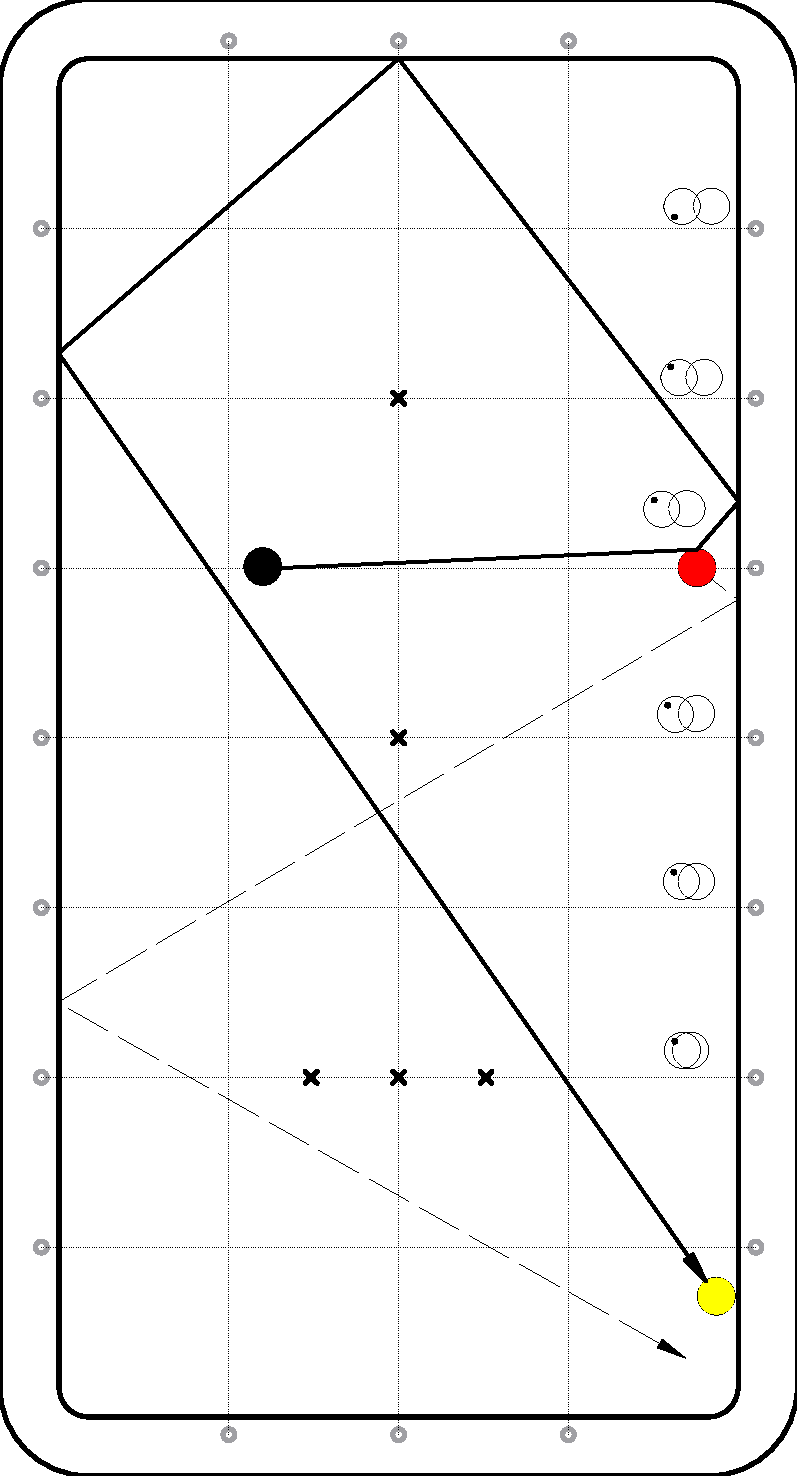
\includegraphics[width=0.85\linewidth]{A/imagesA/A19-01.pdf}
	\caption{Le Carrousel}
	\label{fig:a19-1}
\end{figure}
\clearpage

% !TeX spellcheck = fr_FR
% !TeX encoding = ISO-8859-1

\section{Rappel par deux bandes}

Ce point semble facile et il l'est. Cependant, pour ramener la 2 dans le
� chapeau �, il demande une grande attention et un bon tour de main. Le
danger vient de la bosse possible de la 2 sur la 1, apr�s deux bandes.

Figure : le point se joue en trois quarts coul�, coup allong� et tr�s
accompagn�, peu ou pas d'effet favorable. La difficult� est la juste
prise de la 2. Prise trop fine, la 2 reste en chemin et ne rentre pas.
Prise trop grosse, la 2 risque de percuter la 1 en deux endroits : voyez
les croisements de trajectoires, particuli�rement le deuxi�me. Une bonne
allonge, donne un peu plus de vitesse � la 1 et permet de ramener sans
bosse.

Le tout est une question de mesure et ... d'entra�nement.

Entra�nement : Comme sur la figure, je conseille de commencer avec la 2
en face de la mouche 3. C'est cet emplacement qui est le plus dangereux
pour la bosse. Une fois cette position acquise, essayez des s�ries avec
la 2 en face de la mouche 2, puis en face de la mouche 1. Vous
constaterez par vous-m�me que plus la 2 est situ�e � haut �, moins
grosse (mais au moins une demi-bille) doit-elle �tre prise pour assurer
le point mais alors, la 2 rentre moins bien ! Pour quand m�me rentrer la
2, il y a deux solutions, soit allonger un peu moins ou jouer plus sec :
Ces derni�res nuances sont difficiles d'application surtout si on ajoute
que pour assurer le retour de la 2, la 1 arrive plus rapidement et
risque de ne pas rester dans le secteur, voire d'�clater la 3. Apr�s ces
brillants essais, on peut encore tenter le coup avec la 2 en face de la
mouche 4. C'est difficile et il ne faut pas descendre au-del�. Il s'agit
d'un vrai coul� sans effet, avec la 1 qui doit absolument passer devant
la 2 avant de toucher la petite bande oppos�e.

Cas particulier : Si la 3 est situ�e � une mouche du coin, le m�me coup
est encore possible avec un l�ger effet contraire haut de bille : plus
facile qu'il n'y para�t.

\begin{figure}[htb]
	\centering
	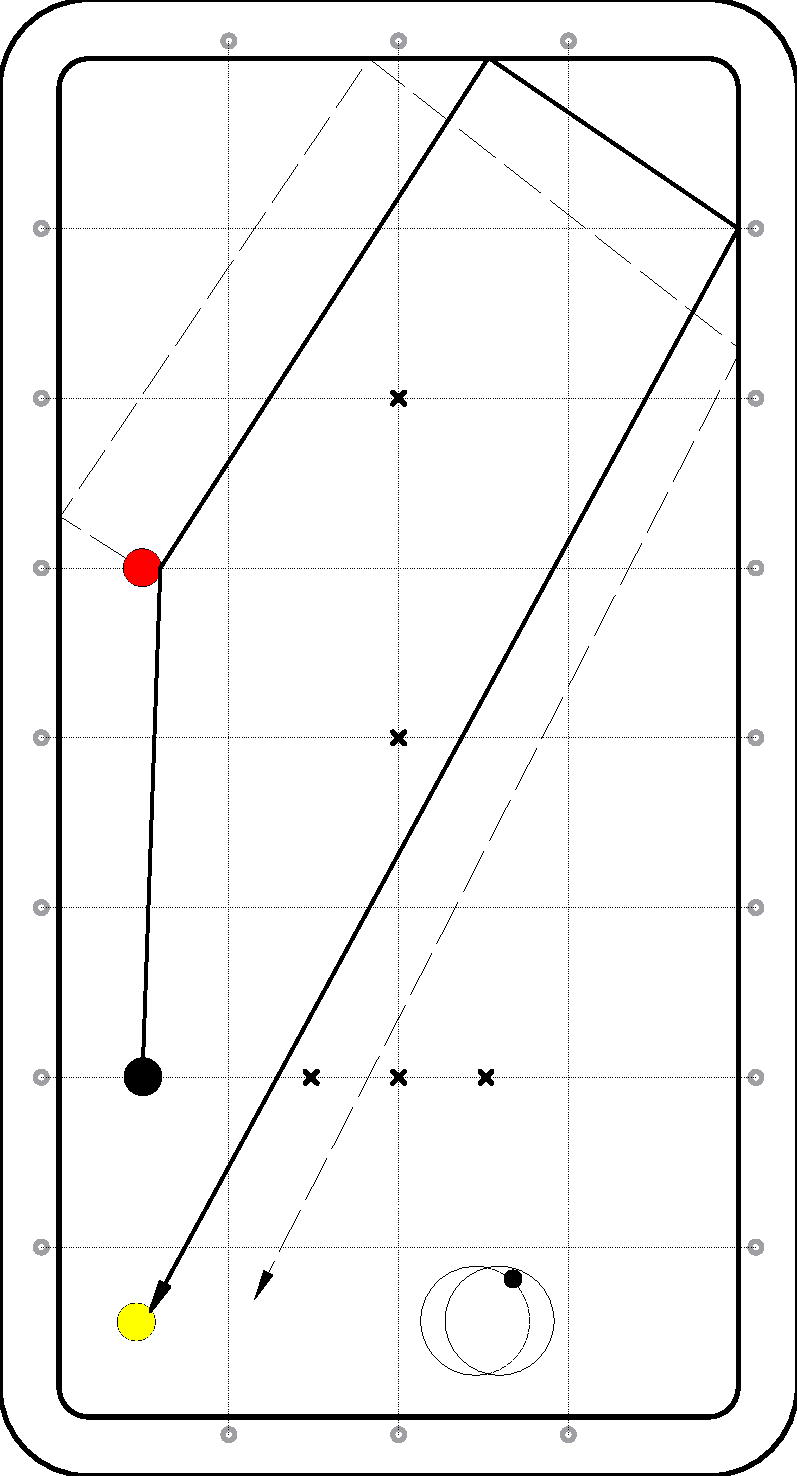
\includegraphics[width=0.85\linewidth]{A/imagesA/A20-01.pdf}
	\caption{Rappel par deux bandes}
	\label{fig:a20-1}
\end{figure}
\clearpage

% !TeX spellcheck = fr_FR
% !TeX encoding = ISO-8859-1

\section{Le Point de Finesse}

Le point de finesse fait souvent peur. Quelques \textless{}\textless{}
trucs � peuvent aider � se donner confiance. Deux � grands cas � peuvent
se pr�senter :

Figure 1 : Les billes 2 et 3 sont tr�s proches l'une de l'autre et la 1
est �loign�e :

\begin{itemize}
	\item
	Examiner attentivement l'angle form� par les directions 2-3 et 1-2. Si
	cet angle est sup�rieur, �gal ou l�g�rement inf�rieur � 45� et si les
	billes 2 et 3 ne se touchent pas, jouez un simple 45�, c�d en
	demi-bille. En effet, il s'agit ici d'une fausse finesse. Si les
	billes faisaient les m�mes angles en �tant �loign�es l'une de l'autre,
	vous n'h�siteriez pas. Vous n'y verriez pas une finesse : n'en faites
	donc pas !
	\item
	Si l'angle pr�cit� est de 45� ou l�g�rement inf�rieur, vous pouvez
	jouer une demi-bille sur la 3 (!). Et oui, en visant une demi-bille
	sur la 3, la 1 touchera la 2 au passage. Votre fixation sur la 3
	�cartera la peur de viser sur la 2 ... (c'est un truc). Aucune
	inqui�tude � avoir. L'exp�rience le prouvera.
	\item
	Si l'angle pr�cit� est nettement inf�rieur � 45�, on peut encore
	rep�rer la portion de la 3 � toucher de mani�re � fr�ler la 2 au
	passage : donc encore rep�rer sur la 3.
\end{itemize}

Figure 2 : Les billes 1 et 2 sont tr�s proches l'une de l'autre.
Examiner d'abord, si la tangente commune int�rieure aux billes let 2
laisse la 3 bien visible ou bien la � coupe �, laissant visible, par
exemple, au moins une demi-bille � 30 cm. ou m�me moins, suivant la
facult� du joueur. En fait, c'est v�rifier qu'en jouant en ligne droite,
sans que la 2 n'op�re une d�viation de la 1, la 3 serait touch�e. Il
faut bien se dire dans sa t�te que la prise en finesse de la 2 est chose
ais�e. On s'attachera � jouer presque � c�t� de la 2, � la limite, visez
avec un seul ?il pour � prendre � le millim�tre qu'il faut et ... ne pas
regarder la 3 ... et jouer doucement pour ne pas accentuer l'angle ...
et ne pas mettre d'effet inutile ! On voit souvent des joueurs appliquer
un effet c�t� 2 : attention ! �a agrandit l'angle. Cet effet convient
lorsque vraiment trop proche de la 2, la pouss�e de la 1 risque de nous
faire faire un queut�. Dans ce cas oui, l'effet � contraire � fait
�viter le queut�. Mais attention, le bon effet provoque ce queut� car,
lors d'un touch� avec effet, le proc�d� reste en contact du c�t� oppos�
de l'effet appliqu� le temps d'une l�g�re d�viation de la bille pouss�e,
avant que celle-ci ne prenne la direction voulue, et on se trouve tout
�tonn� lorsqu'un arbitre nous arr�te pour ce que nous croyons �tre une
injustice alors qu'en fait, nous avons devant nous, un arbitre rigoureux
qui sanctionne notre distraction.

Remarque : Le point de finesse nous invite � jouer un point de vis�e sur
une bille en n�gligeant l'autre bille. Jouez doucement, de mani�re � ne
pas �vaser l'angle au moment du toucher ! Et surtout : ne pas avoir peur
!

\begin{figure}[htb]
	\centering
	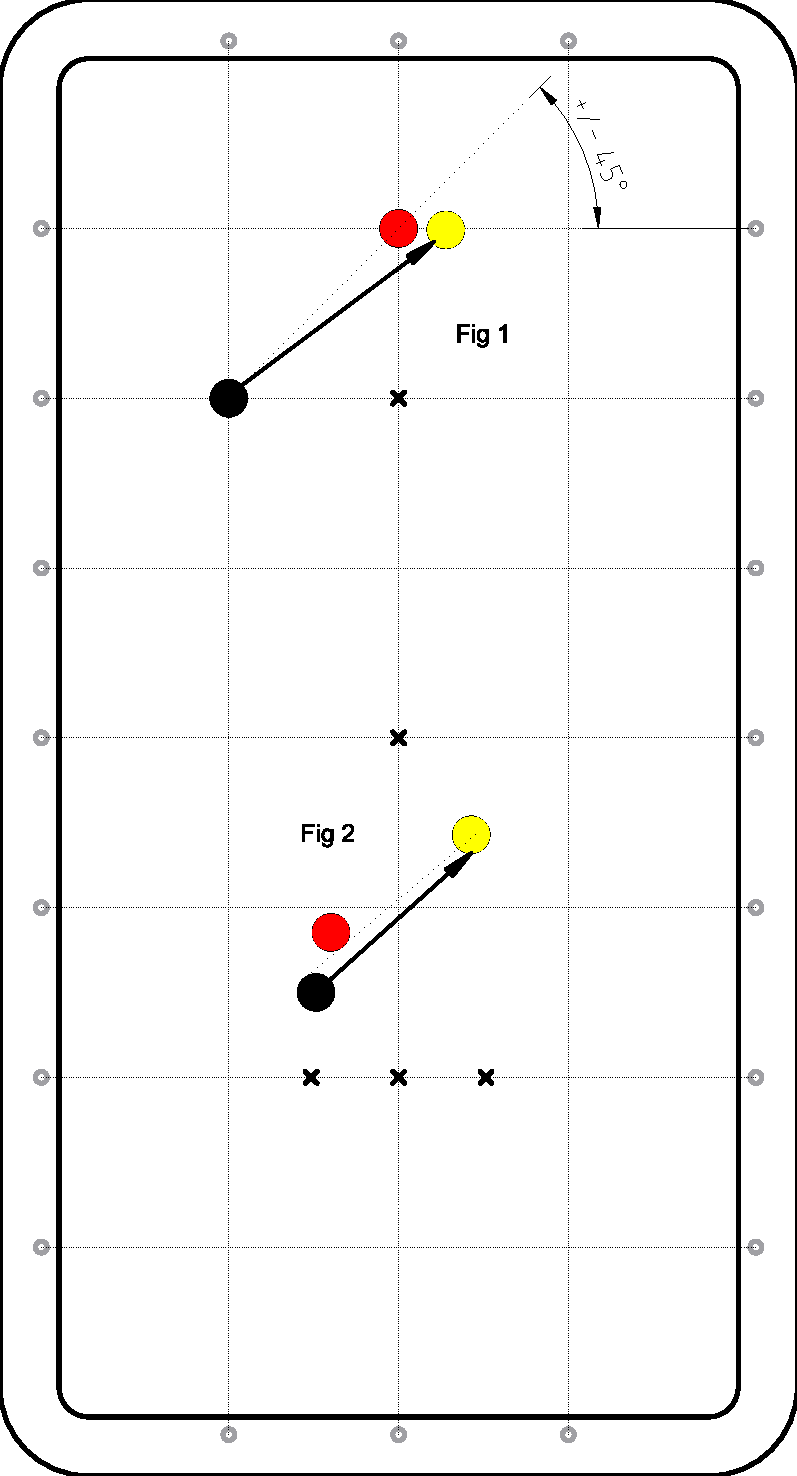
\includegraphics[width=0.85\linewidth]{A/imagesA/A21-01.pdf}
	\caption{Le Point de Finesse}
	\label{fig:a21-1}
\end{figure}
\clearpage

% !TeX spellcheck = fr_FR
% !TeX encoding = ISO-8859-1

\section{Le long coul�}

Le long coul� fait souvent peur et on a raison. Il demande une grande
pr�cision et une tenue de canne ferme et bien rectiligne parce que le
coup port� est tr�s violent. La moindre erreur est multipli�e par un
facteur incertain.

Figure : dans ce cas, le coup est haut, tr�s allong� et tr�s fort,
violent m�me. L'effet est de pr�f�rence � droite avec une prise pleine,
avec seulement une nuance � droite. L'effet �carte un peu la 2 de la
trajectoire d'un contre �ventuel et la force du coup permet le rappel en
doubl� de la 2. Si la position des billes le permet, on peut aussi
appliquer un effet � gauche qui aura pour r�sultat de mieux serrer la 2
vers le jeu. Cependant, vu la difficult� du point, il est souvent
pr�f�rable de lui choisir un effet c�t� grande bande proche, ici �
droite. On augmente nos chances de r�ussite. Celui-l� fait s'�carter la
2 et si nous ne sommes pas tout � fait droit, deux cas peuvent encore se
pr�senter et nous sauver :

1 - : La 1 passe � gauche de la 3. Gr�ce � l'effet � droite, la 1 va �
casser � le coin derri�re par petite bande, grande bande et revient sur
la 2. La mise est sauv�e.

2- ; La 1 passe � droite de la 3. Gr�ce � l'effet � droite, la 1 ex�cute
un renvers� derri�re la 2 par la grande bande, petite bande et re-grande
bande avant de toucher la 2 par derri�re. La mise est encore sauv�e.

Remarque : gr�ce � l'effet, nous assurons une seconde chance de r�ussite
si la 1 passe � c�t� de la 2. C'est une double chance. Nous jouons avec
la possibilit� que les probabilit�s nous donnent. Ce point si difficile
devient un point de difficult� moyenne. Il ne faut cependant pas trop
tenter le diable. Si l'erreur est trop grande, la 1 ne se rattrapera pas
\ldots{} et la 2 non plus.

\begin{figure}[htb]
	\centering
	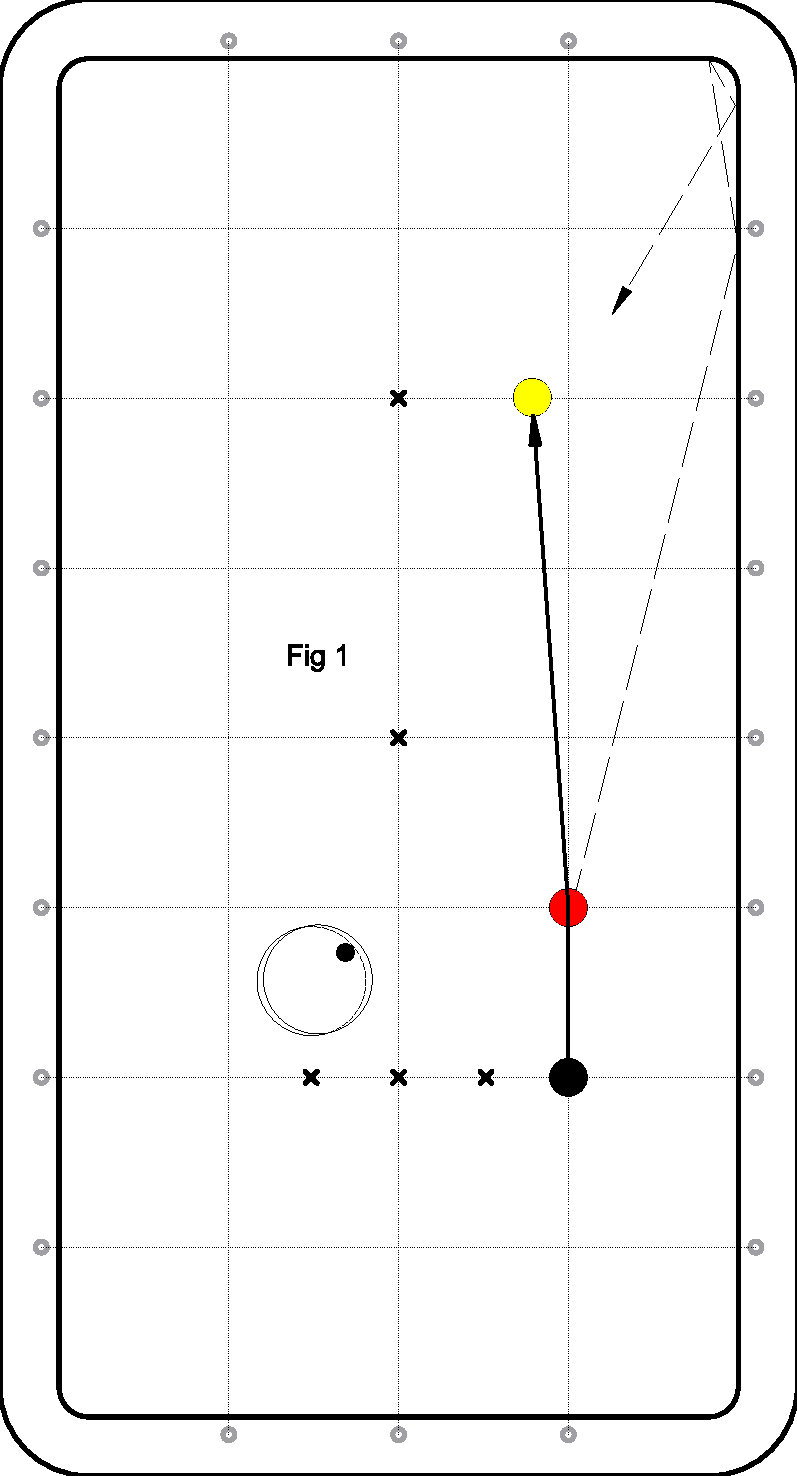
\includegraphics[width=0.85\linewidth]{A/imagesA/A22-01.pdf}
	\caption{Le long coul�}
	\label{fig:a22-1}
\end{figure}
\begin{figure}[htb]
	\centering
	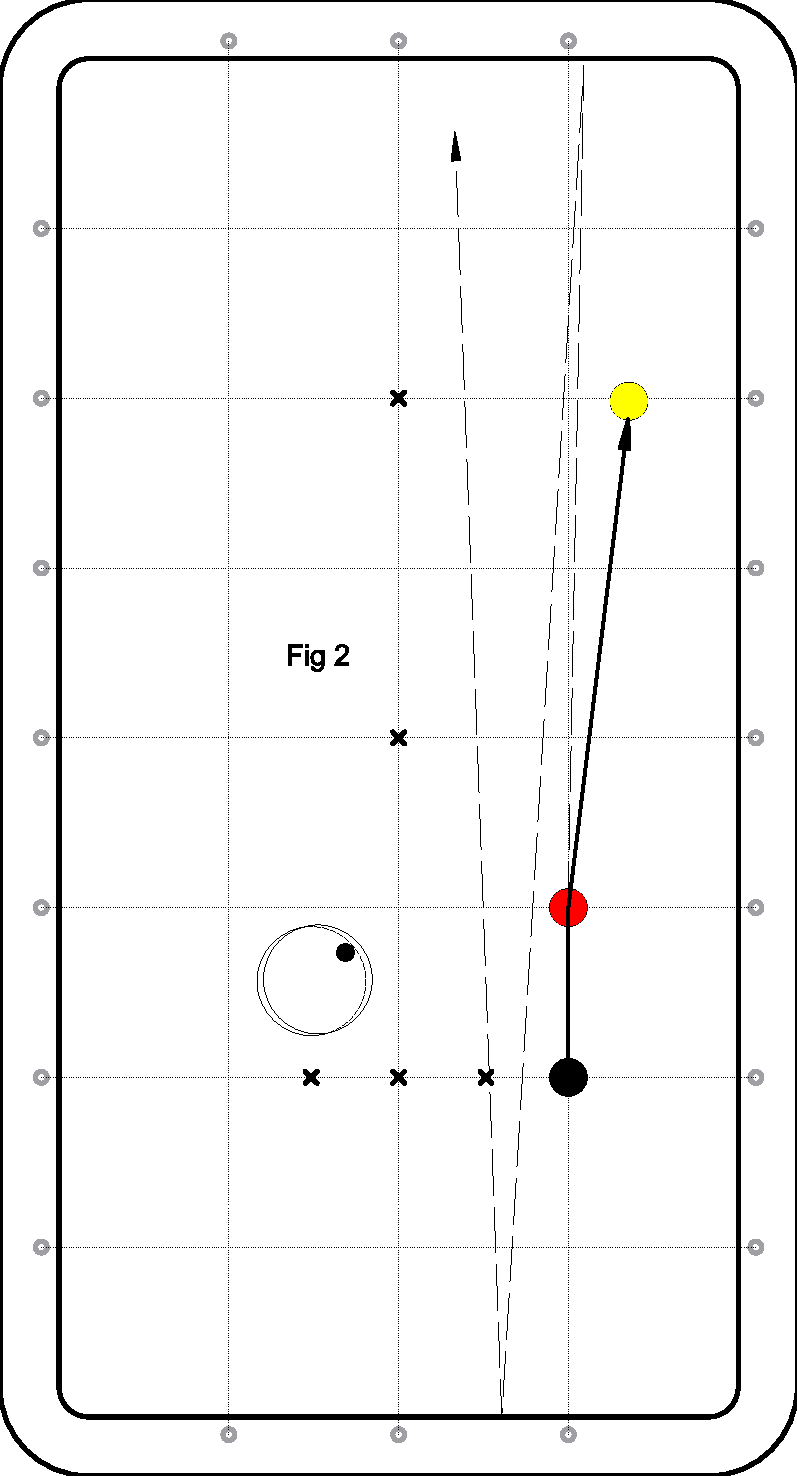
\includegraphics[width=0.85\linewidth]{A/imagesA/A22-02.pdf}
	\caption{Le long coul�}
	\label{fig:a22-2}
\end{figure}
\clearpage

% !TeX spellcheck = fr_FR
% !TeX encoding = ISO-8859-1

\section{Petit R�tro - Long D�placement}

Ce petit point demande une bonne souplesse et une bonne confiance en
soi. La prise est celle d'un r�tro classique. Une r�gle ou bien un truc
� bien assimiler : plus la 2 est proche de la 1, plus la fl�che sera
courte, plus la 3 est �loign�e, plus la main arri�re est loin... Ce
n'est �videmment pas une r�gle absolue et vous verrez � l'usage, qu'il
est possible de la transgresser avec un bon r�sultat. Cette r�gle doit
vous aider � placer les mains sur la canne. La portion de la canne
comprise entre les mains et celle au-del� de la main arri�re constituent
un rapport calculable proportionnel � l'�nergie donn�e au d�part � la 1.
C'est donc tr�s important mais pour l'heure, nous appliquerons la r�gle
que j'ose r�p�ter : Petit d�placement : petite fl�che et long R�tro :
main arri�re loin... C'est ce qu'il faut appliquer ici, on l'aura
compris. On veillera � � bien laisser travailler �\textgreater{} la
canne elle-m�me, presque comme si les mains n'�taient pas l�, comme si
elles �taient l� uniquement pour soutenir la canne dans la bonne
direction sans la serrer ! Nous laissons travailler la canne (hum !)...
Quand on poss�de ce coup, le rythme de la 1 est assez spectaculaire,
comme si elle d�marrait seule, comme si elle avait une volont�. Avec
l'habitude et pour certains, le moelleux du mouvement charmera le
spectateur.

Entra�nement : Placer la 2 � 5 cm de la 1, puis 4, puis 3, puis 2, puis
1 et la 3 � 30 ou 40 cm � l'arri�re de la 2. Essayer des s�ries de 10 �
chaque distance jusqu'� une rentr�e en � chapeau � r�ussie � 90\%.
Essayer le retour � gauche et � droite. C'est fastidieux mais ce sera
payant. Remarque : Le queutage est tr�s dangereux. En fait, il y a
rarement queutage mais bien double touche. Que risque-t-il de se passer
? Au moment du toucher, la canne reste tr�s peu de temps en contact avec
la 1, le temps de parcourir 2 ou 3 millim�tres, tout au plus, rester
plus longtemps serait d'ailleurs consid�r� comme faute. Au contact de la
2, la 1 subit carr�ment un arr�t avant d'effectuer le r�tro. Si la canne
n'a pas �t� arr�t�e � temps, celle-ci re-percute la 1 en bas de bille et
la soul�ve. La 1 retouche alors la 2 sans avoir les � pieds au sol �
avec ce bruit caract�ristique bien connu des joueurs qui croient que ce
seul bruit constitue la preuve de la faute. Cela va tr�s vite et
souvent, le joueur lui-m�me ne sent pas le double coup.

Et l'arbitre ? : L'arbitre doit se placer de c�t�, de mani�re � bien
voir le mouvement de la 1. Ne pas se fier au bruit seulement ! Le bruit
doit constituer une confirmation de ce que l'?il a vu et ne constitue
pas seul, une preuve. Ce bruit provient du fait que la 1 et soulev�e.
Apr�s le choc de la 1 sur la 2, si la 1 s'arr�te, red�marre vers
l'avant, s'arr�te � nouveau, puis seulement effectue son mouvement
arri�re, il y a faute. En g�n�ral, si le point est tr�s court et fautif,
la 1 se soul�vera au deuxi�me contact de la canne. C'est tr�s visible vu
de c�t�. Le placement de l'arbitre est donc capital et les avis des
spectateurs experts qui se trouvent parfois loin de l'aire de jeu sont
souvent sans valeurs ; on les d�pistera facilement au fait qu'ils
affirment mais n'ont pas d'argumentation... Soyez ferme si vous avez ou
croyez avoir vu. Dans la majorit� des cas, il y aura toujours discussion
et ... mati�re � discussion.

\begin{figure}[htb]
	\centering
	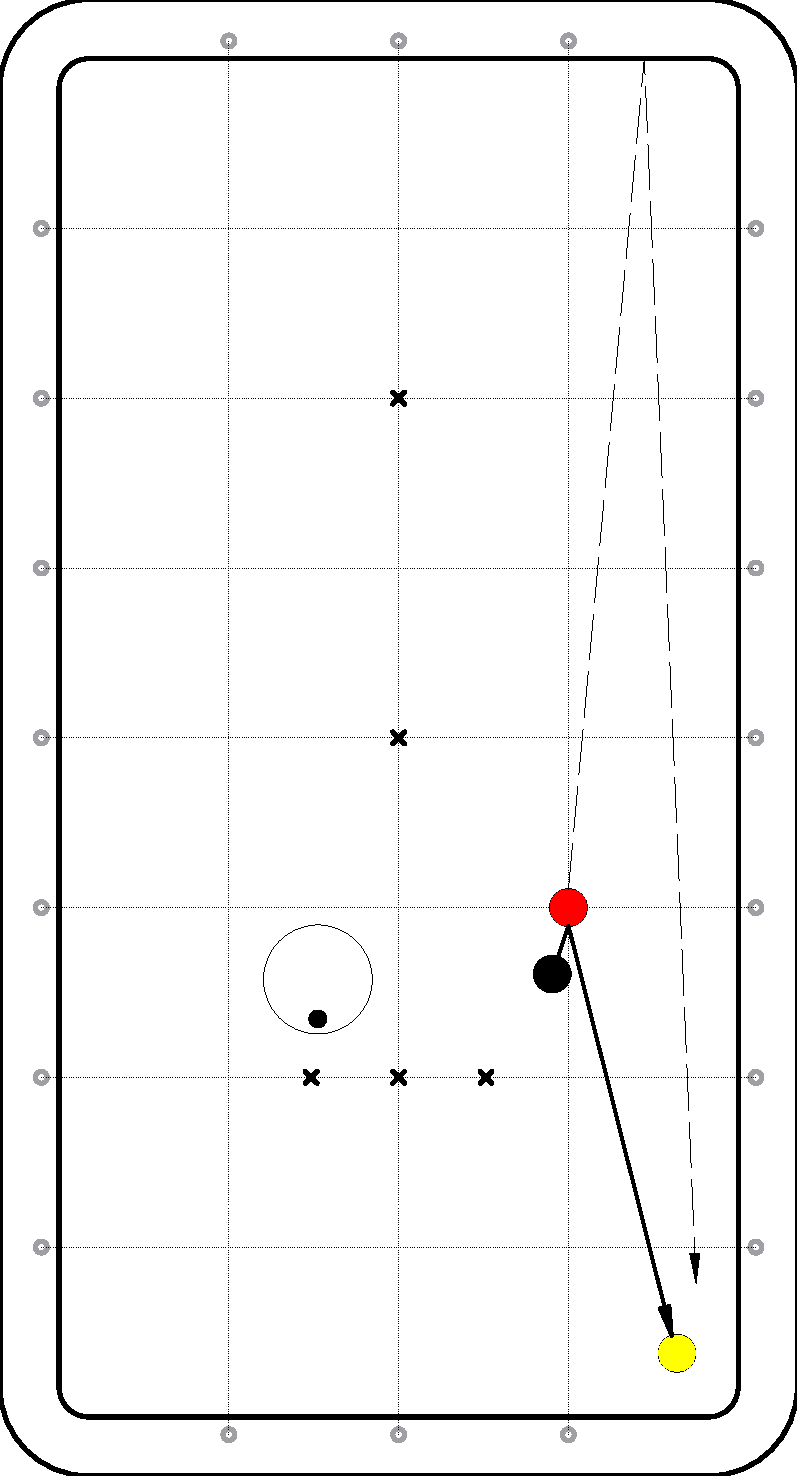
\includegraphics[width=0.85\linewidth]{A/imagesA/A23-01.pdf}
	\caption{Petit R�tro - Long D�placement}
	\label{fig:a23-1}
\end{figure}
\clearpage

% !TeX spellcheck = fr_FR
% !TeX encoding = ISO-8859-1

\section{Le Point Mouche}

Dans tous les matches et � tous les modes de jeu, except� l'artistique,
ce point est le premier � r�aliser. La 1 doit obligatoirement percuter
la rouge en direct, c�d sans l'aide d'une bande. Le joueur peut d�cider
de faire placer sa bille de d�part sur la mouche gauche ou droite par
l'arbitre. Une partie commence par le � tir� � � bande. L'arbitre place
les billes des joueurs au niveau des mouches de d�part. Les deux joueurs
� tirent � vers la petite bande oppos�e. Au retour des billes, le joueur
qui poss�de la plus proche de la petite bande peut choisir s'il commence
ou s'il laisse la place � son adversaire. Attention, d�s que le � tir� �
est lanc�, la partie est commenc�e. Si le � tir� � n'est pas correct,
l'arbitre le fait recommencer. Les raisons d'incorrection sont multiples
: la bille d'un des deux joueurs a touch� la petite bande oppos�e avant
que la bille de son adversaire ait d�marr� ou bien les deux billes se
sont heurt�es ou bien une bille a touch� une grande bande ou bien une
des billes n'a pas touch� la petite bande oppos�e, etc. Par contre si un
� fantaisiste � trouve bien de � doubler � sa bille, le choix revient �
son adversaire. Apr�s le tir�, l'arbitre essuie encore une fois les
billes, les place sur mouche et d�clare la partie commenc�e... Bien que
ce point soit le seul qu'on est certain de rencontrer, il est souvent
rat�...

Le point mouche est difficile mais bien r�ussi, il donne d�j� une
possibilit� de s�rie. Aux trois bandes, il se joue un peu fort de
mani�re � allonger les trois billes le long d'une grande bande. Aux
autres modes de jeu, il se joue plus doux, plus souplement. Il faut
toujours l'essayer avant une partie pour reconna�tre les
caract�ristiques du billard. Laissons le trois bandes aux sp�cialistes.
C'est un coul� ! En th�orie, prendre la 2 en trois-quarts coul�. La 1
casse le coin gauche et revient par trois bandes. La 2 s'arr�te en bas
du billard. Le point se joue en trois bandes � s�ches � car, une fois la
3 manqu�e, la 1 ne reviendra jamais. Il y a risque de contre entre la 1
et la 2 le long de la grande bande droite. Ce contre est la preuve qu'on
avait pris la 1 correctement mais nous devons passer la main ! Ajoutez
une nuance haute ou basse selon qu'on a contr� par devant ou par
derri�re. En fait, il faut essayer selon la table ! De m�me, si on passe
au-dessus de la 3, allonger un peu, si on passe en dessous de la 3,
allongez moins. Mon truc : Je vise la 2 y pla�ant dans ma vis�e la
pointe de ma fl�che en tangence int�rieure c�t� gauche. Ensuite, je fais
glisser ma canne parall�lement � sa position de d�part jusqu'� pointer
au centre du secteur sup�rieur droit de la 1. Selon le r�sultat apr�s
l'essai, je vais rapprocher la fl�che du centre de la bille ou bien du
diam�tre horizontal ou les deux... Une fois le r�sultat correct, je
m�morise la position de ma fl�che par rapport � la bille 1 et
l'intensit� de p�n�tration (allongement). Ce point demande beaucoup
d'entra�nement jusqu'� ce que la 1 percute la 3 doucement .... (juste le
chemin) et que la 2 se blottisse � la petite bande. Composer avec tous
les param�tres en pr�sence n'est pas chose ais�e. Un long et acharn�
travail sera tr�s utile.

Bonne Chance !

\begin{figure}[htb]
	\centering
	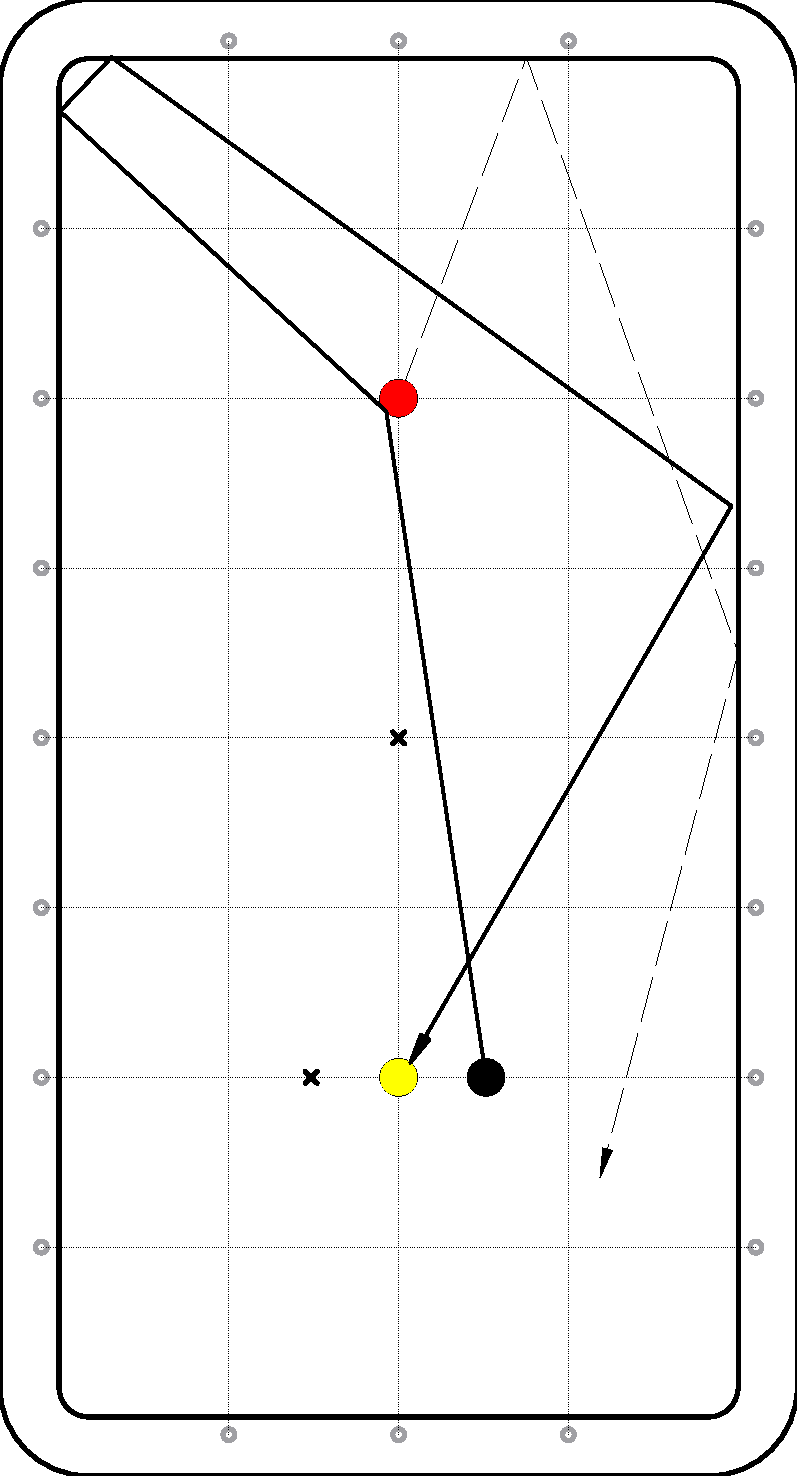
\includegraphics[width=0.85\linewidth]{A/imagesA/A24-01.pdf}
	\caption{Le Point Mouche}
	\label{fig:a24-1}
\end{figure}
\clearpage


\chapter{La technique}
\newpage

% !TeX root = ../book.tex
% !TeX spellcheck = fr_FR
% !TeX encoding = ISO-8859-1

\section{Le Deux Bandes}


Ce point se pr�sente souvent lors du d�roulement d'une partie. Il est de
premi�re importance car il pr�sente souvent une position de rappel en
deux coups. Quoique de r�alisation facile, il est souvent mal ex�cut�
voire rat�. Ne le n�gligez pas. N'ayez pas peur de prendre votre temps
et de bien r�fl�chir avant de porter le coup.

Examinez la figure ci-contre. Nous sommes en 1, � en dehors � des billes
2 et 3 c�d que je << vois >> les deux autres
billes... qui sont r�parties de part et d'autre de la bissectrice de
l'angle du coin. 1 - Rep�rez le point � B � situ� � �gale distance des
billes 2 et 3 ou si on pr�f�re une autre formulation : consid�rez le
milieu du segment de droite reliant la 2 et la 3. 2 - Tracer mentalement
une droite passant par le point B que nous venons de d�terminer et le
coin �C�. 3 -- Tracer une droite tangente int�rieure � la 2 et parall�le
au segment BC. 4- Cette derni�re droite coupe la petite bande au point
R. Ce point R devient notre point de rep�re rapproch�. 5 -- Il reste �
r�aliser le point. Ne consid�rons plus la bille 3 mais bien le point R
comme �tant le c�t� ext�rieur de la 3, celle-ci imagin�e situ�e en
direction de l'axe du coin C et tangente au point R. On a donc
transform� un deux bandes en une � lunette �. On ne regardera plus la 3,
pour se concentrer uniquement sur la 1 et le point R. Le coup est port�
avec un effet favorable haut de bille sur la premi�re bande touch�e. Le
coup aura la force suffisante pour repousser la 3 de 5 � 10 cm de
mani�re � nous procurer une position souvent de r�tro qui nous permet un
regroupement bas de table. 6 - La nouvelle position obtenue sera
g�n�ralement un r�tro direct ou un r�tro bande.

Pr�caution : Les billes 2 et 3 doivent �tre de part et d'autre de la
bissectrice de l'angle du coin sinon le calcul devient n�gatif et les
r�sultats tout � fait faux. La 1 doit �tre � � l'ext�rieur � des billes
2 et 3, quoique le calcul reste bon mais si la bille est � int�rieur �,
le coup droit doit �tre chang� pour un r�tro et la port�e de l'effet
modifie le calcul. Contentons-nous de ceci pour le moment.

Remarques : Ce truc n'est g�om�triquement pas exact. Il offre une erreur
de une bille pour une demi table. Il n'est donc plus valable si les
billes occupent le bas et le haut de la table.

Encouragement : Le calcul semble bien compliqu�. � l'usage, vous
constaterez que sur le terrain, il vous para�tra beaucoup plus �vident.
Bien en possession de cette technique, vous y serez rapide et ce point,
devenu inratable, vous am�nera de l'assurance.

\begin{figure}[htb]
	\centering
	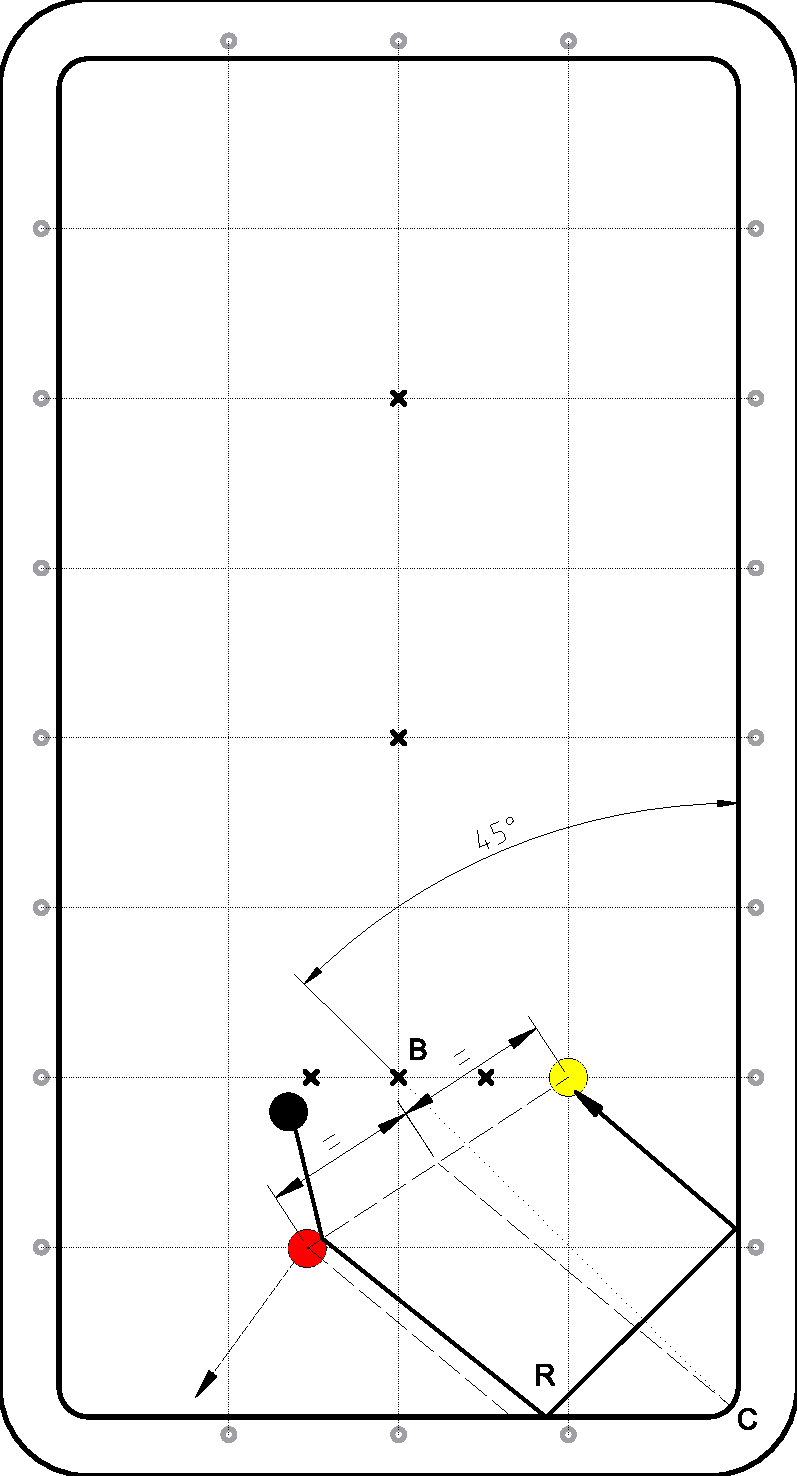
\includegraphics[width=0.85\linewidth]{B/imagesB/B01-01.pdf}
	\caption{Le Deux Bandes}
	\label{fig:B01-1}
\end{figure}

\clearpage


% !TeX root = ../book.tex
% !TeX spellcheck = fr_FR
% !TeX encoding = ISO-8859-1

\section{Anti-Rappel - Deux Bandes}

Attention : ce point ressemble au pr�c�dent (B01) mais il n'est pas le
m�me. Je l'appelle anti-rappel parce que le repositionnement n'est pas
s�r et la 1 non dominante, se place souvent au milieu des deux autres
billes. Bien que le jeu s'en trouve serr�, on devra faire tr�s attention
si une autre solution n'�tait pas plus profitable, un direct ou un coul�
par exemple...

Voyez la figure : Comme pour B01, estimez le milieu du segment qui joint
les billes 2 et 3. Soit le point A. Tracez une droite passant par A et
le coin voisin. Tracez une droite parall�le � celle-ci et passant par la
bille 2, soit b qui coupe la bande au point R. Ce dernier devient le
point de vis�e rapproch�. La 1 se touche en t�te, effet favorable � la
premi�re bande, de mani�re � � tanger � le point R (toucher juste
devant). Si la bille 2 est trop proche de la petite bande, il y a risque
de contre de la 1 sur la 2 qu'il est possible d'�viter en tentant un 1
bande ou un deux bandes, m�me prise de bille mais effet inverse (voir
figure en pointill�). Si la bille 2 emp�che le passage, on r�alisera un
direct, trois-quarts coul�, effet inverse � la bande.

Ce rappel des billes donne une position non dominante c�d que la 1 se
trouve du c�t� de la petite bande et les deux autres billes sont situ�es
du c�t� champ; le jeu � monte �. Il reste � juger de cette nouvelle
position avant de choisir, soit un r�tro vers la petite bande oppos�e,
repla�ant une position dominante, soit un r�tro vers la grande bande
oppos�e, repla�ant une position dans le tiers de la table. Il arrive
aussi qu'un simple � passage � donne directement la dominante. Ces choix
d�pendent, �videmment, de chaque situation tant des billes adverses que
de la facilit� � man?uvrer sa propre bille.

Cas particulier :- Si la 2 colle la petite bande ou presque et que la 1
est plus �loign�e de ladite petite

bande que la 2, on peut appliquer un coup dur par trois-quarts coul�,
effet c�t� petite bande. La 2 se voit entra�n�e par le mouvement de la
1. Nous sommes en pr�sence d'un coup bosse classique.

- Si les billes 1 et 2 collent la petite bande ou presque et sont en
alignement presque parfait le long de cette bande, il faut doubler la 2
par un coul� direct en force avec effet du c�t� inverse � la petite
bande de mani�re � �viter le contre de la 2 sur la 1 � son retour.

\begin{figure}[htb]
	\centering
	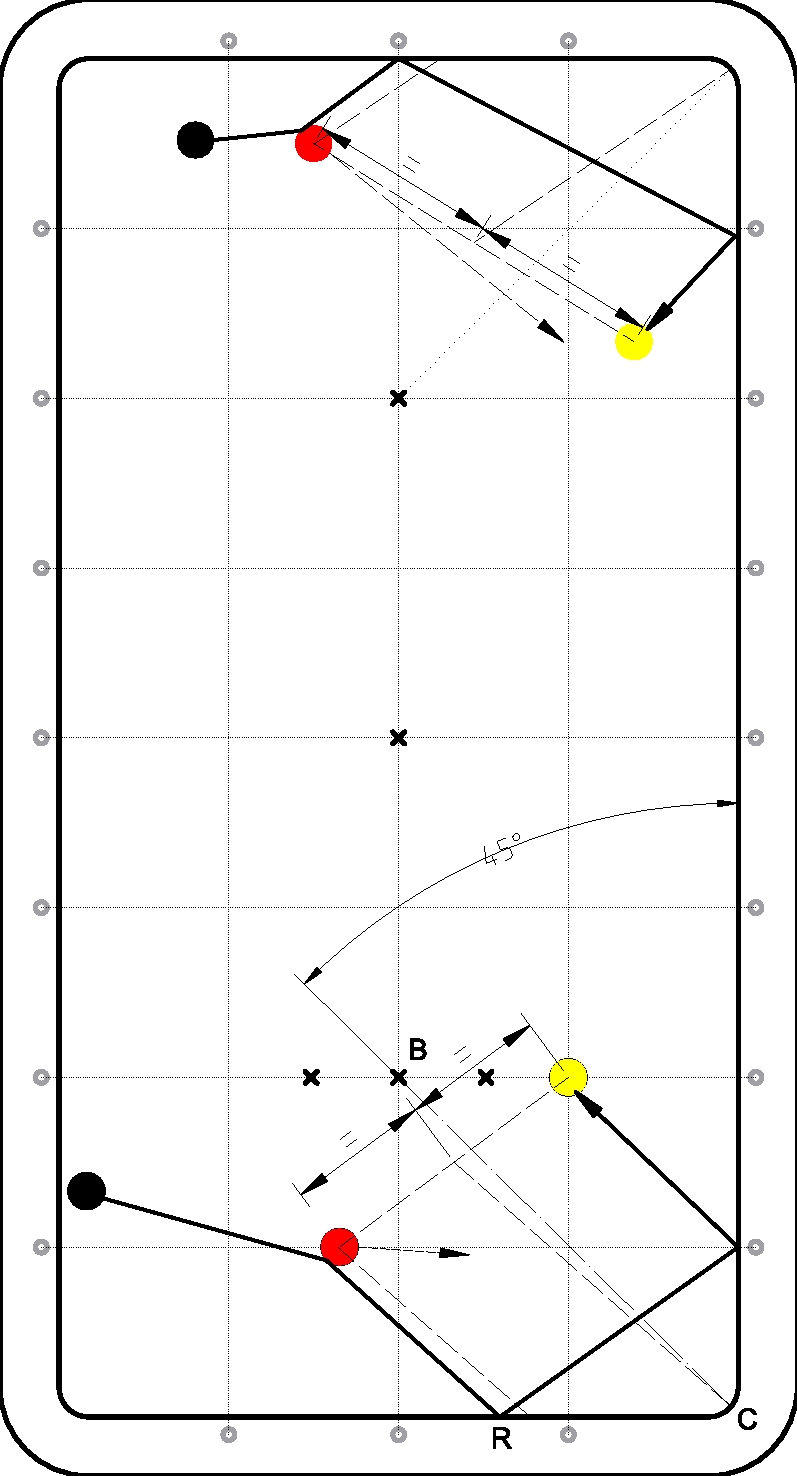
\includegraphics[width=0.85\linewidth]{B/imagesB/B02-01.pdf}
	\caption{Anti-Rappel - Deux Bandes}
	\label{fig:B02-1}
\end{figure}

\clearpage


% !TeX root = ../book.tex
% !TeX spellcheck = fr_FR
% !TeX encoding = ISO-8859-1

\section{Serrage dans le coin par 3	Bandes}

Voil� une position qui est assez fr�quente. L'alignement des billes est
telle qu'une finesse ne peut pas �tre tent�e et un 1 bande par la grande
bande, c'est pratiquement impossible. Le coul� direct fait partir la 3
ou bien permet le point mais la 2 ne reste pas ou contre la 1. Bref, ce
point est bien r�calcitrant. C'est un tra�tre point... et pourtant.

Ne jamais tenter un 1 bande par la gauche via la petite bande. La 2 se
perd dans la nature. On casserait la possibilit� de ramener le jeu dans
le tiers. On pourrait le tenter si la 3 �tait assez proche du coin mais
alors, il s'agirait d'une autre position que celle expos�e ici.

Eventuellement, � condition de s'en sentir capable, on peut choisir un
mass� par la droite. Nous n'avons pas encore parl� du mass�. Ce sera
pour l'ann�e prochaine mais sachez qu'il est int�ressant, si les billes
ne sont pas trop �loign�es, mais reste un point difficile m�me pour les
joueurs aguerris.

Je vous propose deux solutions plus faciles et surtout plus
constructives. 1 - Celle que je pr�f�re est un 3 bandes s�ches (!) par
la droite. Surtout, ne pensez pas aux calculs du 3bandes que certains
vous expliqueront � renfort de preuves. Il s'agit de ramener le jeu et
non de faire un 3B n'importe comment. N�gociez une finesse sur la droite
de la 2 de mani�re � ne pas permettre � celle-ci de s'�vader du coin.
Plus la prise sera fine, plus elle conviendra pour r�ussir � garder la 2
mais plus il faudra appliquer d'effet � droite afin d'aller chercher le
coin diam�tralement oppos�. Souvent, l'effet bas de bille sera
n�cessaire. Attention.... Il est important d'�tre souple afin
d'avantager la vitesse de la 1 plut�t qu'utiliser la force. Au moment de
r�aliser et en position pour jouer, ne pensez qu'� une chose : � Je veux
aller chercher le coin... � 2 - On peut aussi appliquer un coul� en
force apr�s avoir v�rifi� que la 2 ne percutera pas la 3 dans

arse folle et que la finesse choisie au point pr�c�dent offre trop de
difficult�. Ex�cutez donc un coul� en force et en souplesse en
trois-quarts ou quatre cinqui�mes ou m�me plus gros encore avec effet �
droite tr�s imprim�. Comme le montre la figure, la 1 revient en 3 bandes
s�ches ou en 4 bandes. Si possible, nous choisirons le 3 bandes car le 4
bandes offre un danger de contre de la 1 avec la 2 voyageant au fond. A
l'entra�nement, nous v�rifierons bien que la 1 effectue une courbe avant
de tourner... C'est la preuve d'un coul� souple, fort et r�ussi...

Ces deux solutions donnent souvent une position dominante ou une
possibilit� de rappel direct. A choisir, faites la finesse ; on y
ma�trise mieux le mouvement des billes.


\begin{figure}[htb]
	\centering
	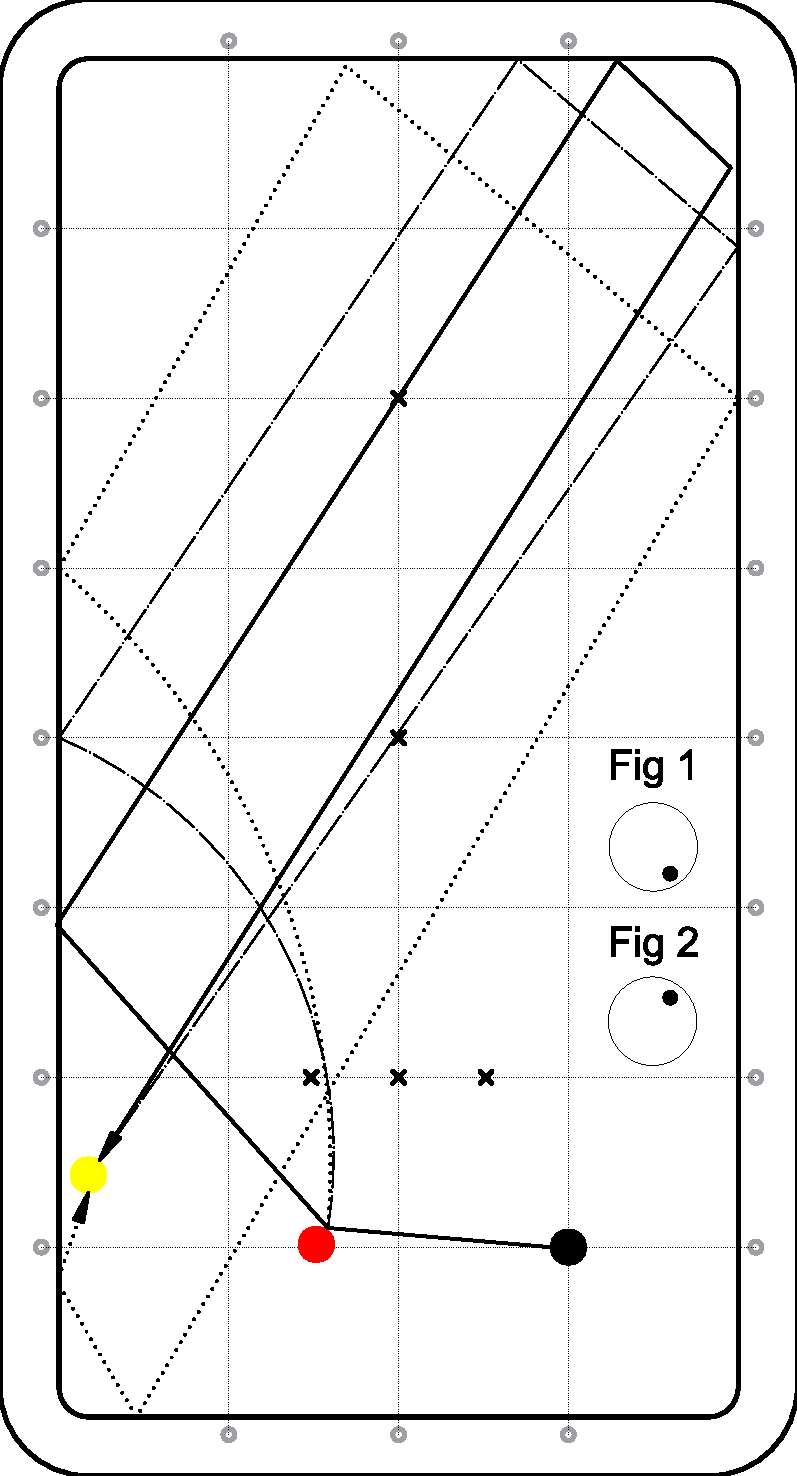
\includegraphics[width=0.85\linewidth]{B/imagesB/B03-01.pdf}
	\caption{Serrage dans le coin par 3 Bandes}
	\label{fig:B03-1}
\end{figure}

\clearpage


% !TeX root = ../book.tex
% !TeX spellcheck = fr_FR
% !TeX encoding = ISO-8859-1

\section{3 billes dans le coin par le tour}

Ce coup doit �tre consid�r� comme facile car il offre une tol�rance
d'erreur importante. Il y a cependant un danger de contre en bas de la
table, si on joue en quatre bandes.

Comme le montre la figure, c'est un trois quarts coul�, effet � droite
en-t�te, souple et allong�. La difficult�, afin de ne pas jouer trop
fort et que la 1 fasse bien le chemin n�cessaire, est de faire confiance
� son mat�riel... faire coulisser la canne de mani�re tr�s r�guli�re, le
coup port� r�sultant d'un limage plus long et non d'un v�ritable coup
port�. C'est plus facile � dire qu'� faire ! Donner confiance � un bout
de bois et perdre ainsi une part de contr�le de nos gestes nous est
presque insupportable. Et pourtant, le bon coup r�sulte d'un certain �
abandon � de soi. Nous devons savoir que cet abandon n'est pas une
renonciation mais l'aboutissement d'un travail constant qui fait passer
la � m�canique � dans les doigts comme un geste que nous faisons
r�guli�rement sans r�fl�chir et qui pourtant, est le geste juste.

Afin de perfectionner ce point, il conviendra de s'exercer � rentrer la
2 dans le coin � c�t� de la 3.

Corrections �ventuelles :

La 2 ne rentre pas au coin mais reste haut sur la table : jouer plus
fin. La 2 touche la petite bande et remonte trop

haut : toucher plus gros et allonger un peu. - La 1 touche la petite
bande (4�bande) trop loin du coin : si la 2 ne rentre pas, on a jou�
trop

gros; si la 2 rentre, il faut jouer plus souplement. La 1 touche la
grande bande (4�bande) trop loin du coin : si la 2 ne rentre pas, on a
jou� trop fin ; si la 2 rentre, jouer plus souplement, plus � abandonn�
�...

Remarque : ce coup fait penser au � carrousel � (A-19). On peut
effectivement le consid�rer comme un perfectionnement du carrousel. La
grande diff�rence est que le carrousel se calcule et que les trois
billes dans le coin par le tour se sentent... C'est un �tat d'esprit qui
s'installe. Ce ramen� est tr�s int�ressant. Il permet de serrer dans le
coin des situations s'�talant sur plus de la moiti� de la table c�d que
sur plus de la moiti� de la grande bande, le jeu peut �tre ramen� dans
le tiers, voire le coin.

Figure : en trait continu, le 3B sec... en pointill�, le 4B.

\begin{figure}[htb]
	\centering
	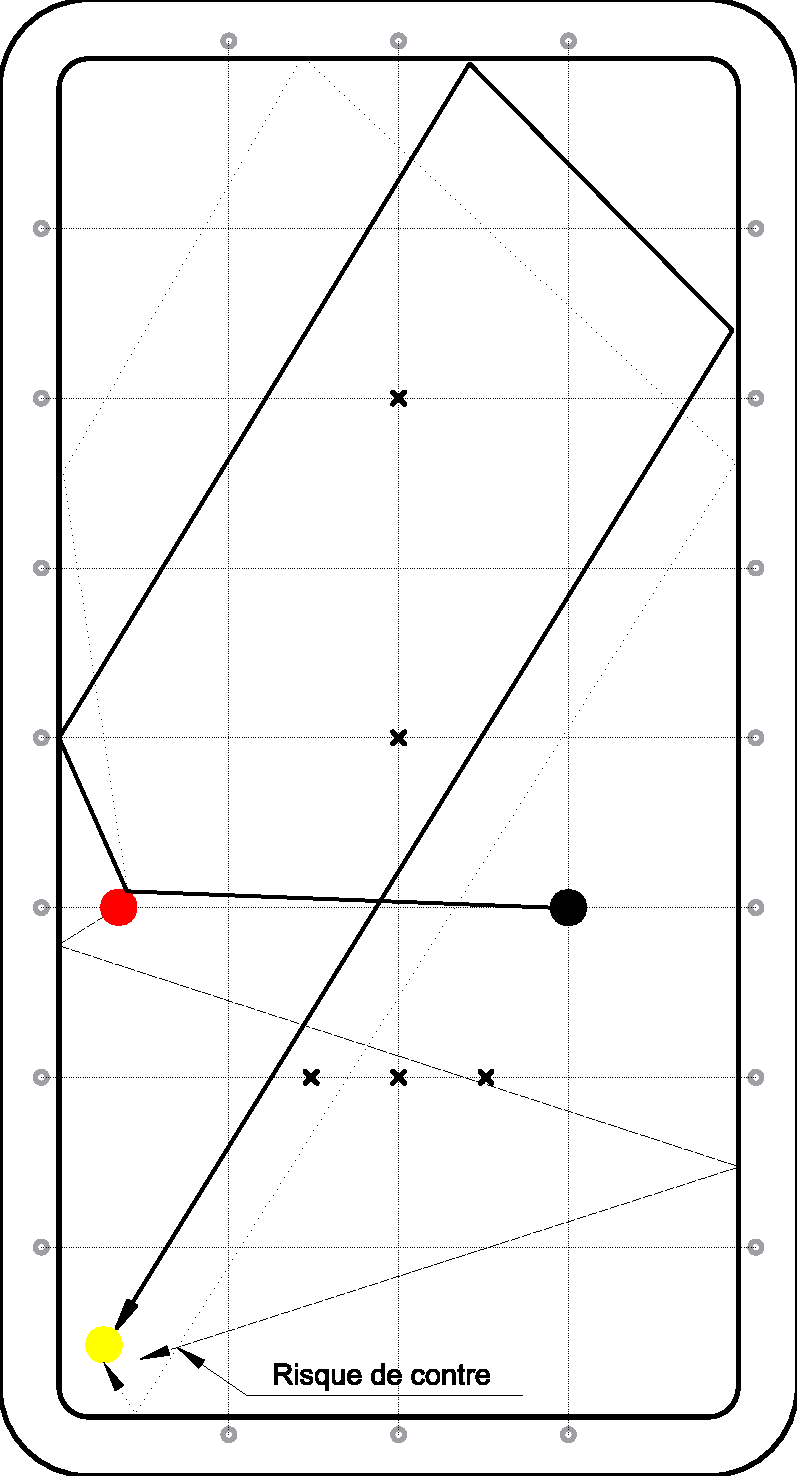
\includegraphics[width=0.85\linewidth]{B/imagesB/B04-01.pdf}
	\caption{3 billes dans le coin par le tour}
	\label{fig:B04-1}
\end{figure}

\clearpage


% !TeX root = ../book.tex
% !TeX spellcheck = fr_FR
% !TeX encoding = ISO-8859-1

\section{3 bandes dans le carr�}

Ce point se calcule comme le deux bandes par le coin (B01), except�
qu'il ne faut pas consid�rer la bille 3 l� ou elle se trouve mais bien
la 3', bille imaginaire et sym�trique de la 3 par rapport � la grande
bande proche. Pour que le calcul soit exact, les restrictions sont les
m�mes que pour un deux bandes par le coin � savoir : les billes doivent
se trouver dans un demi billard sinon l'erreur devient trop grande, et
les billes 2 et 3 doivent se trouver de part et d'autre de la
bissectrice de l'angle du coin.

Consid�rez la figure :

- Imaginez-vous bien la bille 3

sym�trique de la 3. - Prenez le milieu du segment 2-3' d�sign� od

ici en M2. Tracez une droite passant par M2 et le coin C. Tracez une
droite parall�le � la pr�c�dente passant par la 2. Celle-la coupe la
grande bande au point R qui devient notre point de rep�re rapproch�. Il
reste � r�aliser la lunette 2-R ... en n'oubliant pas l'effet favorable
haut de bille.

Autres m�thodes :

Le point M2 �tant difficile � fixer, dans la mesure o� il est interdit
de placer des rep�res sur le billard, tout calcul devant se figurer dans
l'espace et notre vil n'�tant pas toujours fid�le, on peut appliquer la
m�thode de la fiche B01, puis � reculer � le point M1, milieu du segment
2 3 d'autant que la distance de la 3 � la grande bande proche (la moiti�
d'un segment est �gale � la somme des moiti�s des segments qui le
compose) On peut aussi �valuer l'endroit de la grande bande, R' o� notre
bille 1 devrait toucher pour r�aliser et appliquer entre ce point R' et
la 2, la th�orie du B01.

Remarques :

- Ce point constitue un << rester sur le billard >> plut�t qu'un serrage. Bien que pas tr�s

int�ressant, il peut donner des positions d'attente favorables. - En
g�n�ral, choisissez comme � 2 � la bille la plus proche du coin, quoique
si la 2 est trop

proche, on devra faire attention au � contre � de la 2 sur la 1. Lorsque
la bille 2 est trop � haute �, il y a aussi risque de contre de la 2 sur
la 3 et m�me parfois, barrage � la 1. Enfin, pour que le calcul soit
exact, il conviendra que la 1 ne soit pas trop pr�s de la petite bande
du bas, en dehors du � jeu � 2 et 3 ... car un r�tro serait alors
n�cessaire et l'effet du r�tro se marque beaucoup plus fort... Enfin,
chacun choisira sa m�thode, pourvu que le r�sultat soit bon...


\begin{figure}[htb]
	\centering
	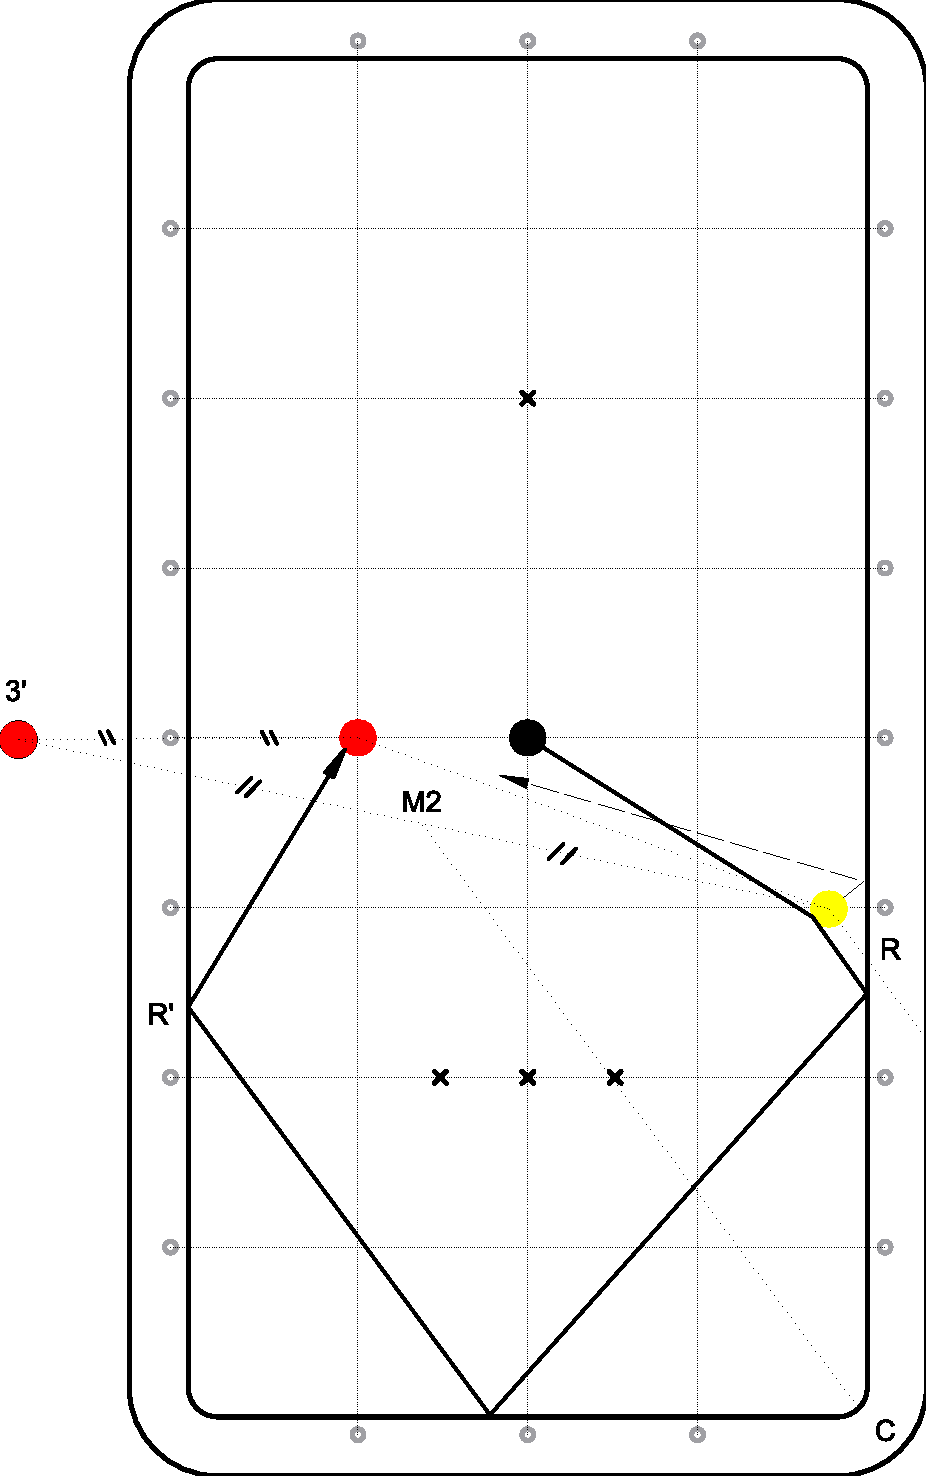
\includegraphics[width=0.85\linewidth]{B/imagesB/B05-01.pdf}
	\caption{3 bandes dans le carr�}
	\label{fig:B05-1}
\end{figure}

\clearpage


% !TeX root = ../book.tex
% !TeX spellcheck = fr_FR
% !TeX encoding = ISO-8859-1

\section{Rappel dans le coin par une Bande}

Voici une s�rie de positions qui se pr�sentent tr�s souvent, dont la
r�alisation est facile et la mani�re importante pour la suite du jeu. Le
principal objectif est de ramener la 2 dans le coin � c�t� de la 3.

Figure 1: c'est la position type. Avec une inclinaison 1-2 de 30�
environ par rapport � la petite bande, prendre la 2 en demi-bille,
allonger comme un coul� et appliquer un peu ou pas de bon effet. La
canne doit �tre absolument horizontale : cela permet de donner de
l'�nergie � la 2 et de revenir au coin sans trop de vitesse.

Figure 2 : La 2 est assez haut le long de la grande bande oppos�e au
joueur. Au fur et � mesure que la bille 2 � monte �, il conviendra de
baisser la prise de la 1 m�me jusqu'au bas de bille avec un effet plus
important. Si l'angle 1-2 / petite bande est trop grand, au-del� de 40�,
il ne sera plus possible de � revenir � par le simple effet. Il
conviendra de baisser la vis�e jusqu'au r�tro ou demi r�tro en ayant
toujours en t�te la grosseur de bille � prendre pour assurer un retour
de la 2 dans le coin o� se trouve la 3.

Figure 3 : La 2 a d�pass� le milieu de la grande bande et se trouve en
haut du billard. Par chance la 1 n'est pas loin de la 2 et forme avec
elle le m�me angle (309) avec la petite bande du bas. R�tro bille bande,
souplesse et coup r�gulier sans heurt : l'�nergie se partage entre la 2
et la 1 et celles-ci reviennent au coin comme se tenant par la main.

Figure 4: La 2 est haute et s'est d�plac�e vers le milieu de la table.
La 1 l'a suivie avec un angle plus petit que celui de base. Pas d'effet,
l�g�rement sous le centre bille. Poussez la 2 sur la petite bande le
plus pr�s possible du coin oppos� � celui de la 3 et touchez la grande
bande avec un angle d'environ 450. Cela veut dire que le coup est un peu
r�tro et un peu � contraire �. C'est un point magnifique qui transforme
une position apparemment perdue en un coup de construction.

Entra�nement : Cela va de soi : il conviendra de faire des s�ries
d'essais avec la 2 qui monte le long de la grande bande oppos�e et
s'�carte vers le milieu, arriv�e en haut. Au d�part, la 1 est comme sur
la figure 1. Au fur et � mesure que la 2 monte le long de la grande
bande, elle s'en rapproche en veillant � l'angle de 30� et le diminue
quand la 2 vire au milieu en s'approchant de la petite bande oppos�e.
Ces essais sont d'une importance capitale pour le jeu de rappel � dans
le tiers �. On exigera une r�ussite � 100 \% pour le point de base et
90\% pour les points du haut de table.

Remarque : attention ! ce point est � essayer avant toute comp�tition
car il permet de juger si les bandes glissent ou pas. L'angle r�sultant
d'une bande glissante est surprenant. Pour r�duire cette � glissade �,
visez moins haut sur la 1 ou rapprochez la vis�e du centre de la bille.


\begin{figure}[htb]
	\centering
	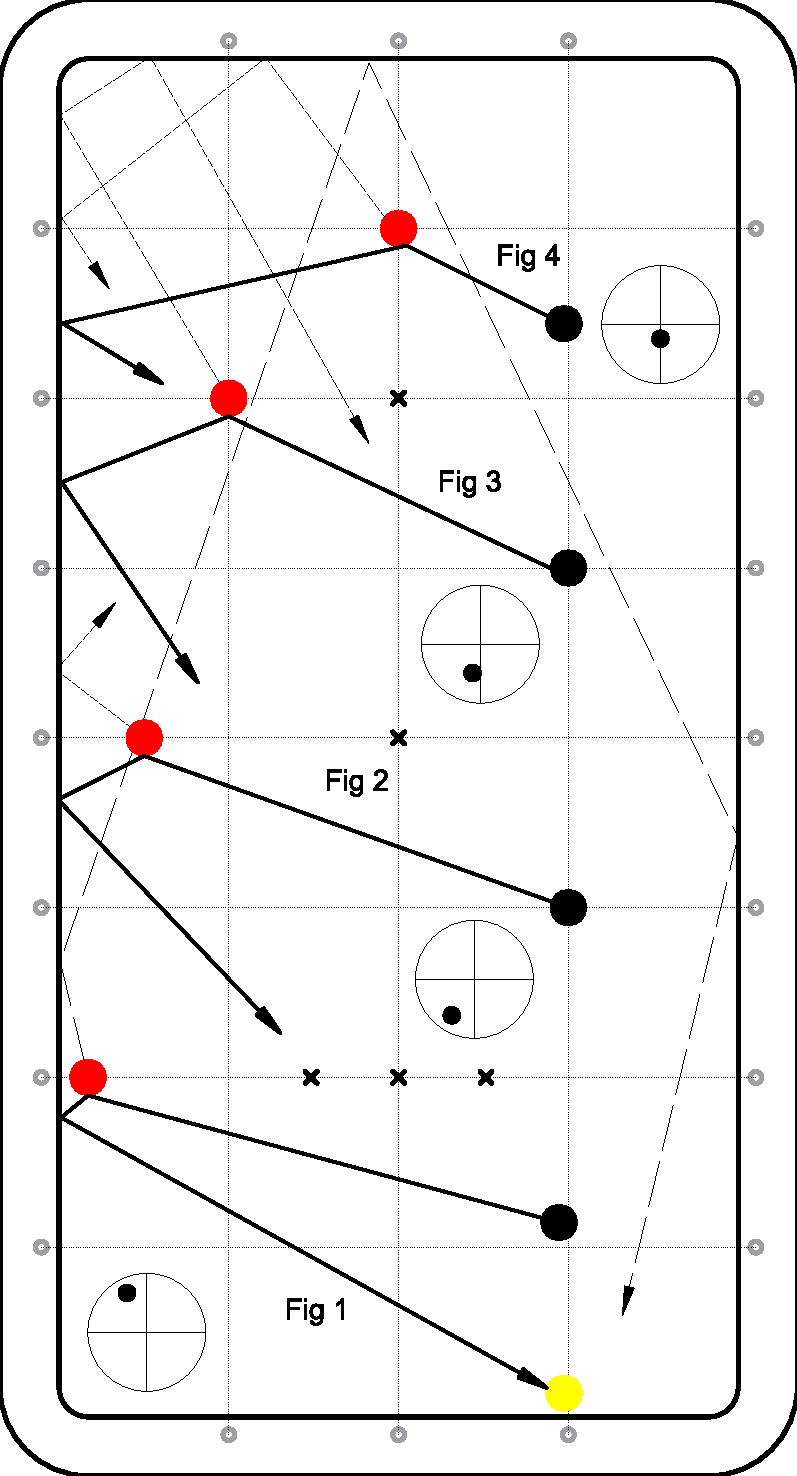
\includegraphics[width=0.85\linewidth]{B/imagesB/B06-01.pdf}
	\caption{Rappel dans le coin par une Bande}
	\label{fig:B06-1}
\end{figure}

\clearpage


% !TeX root = ../book.tex
% !TeX spellcheck = fr_FR
% !TeX encoding = ISO-8859-1

\section{ Rappels extr�mes par une bande}

Le B06 nous a montr� toute une s�rie ou plut�t une famille de positions
tr�s fr�quemment rencontr�e et souvent n�glig�e. On pense souvent
r�aliser le point sans envisager de construire. Sans doute fera-t-on
moins de � brosses � (moins de z�ros) mais on r�alisera aussi moins de
s�ries. Si vous voulez progresser, il faut n�gliger les petites reprises
et la crainte de laisser une bonne position � l'adversaire. Si ce
dernier est en forme, votre d�fense se retournera contre vous et s'il
n'est pas en forme, m�me une bonne position ne l'avantagera pas. Je
conseille donc toujours, de tenter une rentr�e d�s qu'elle repr�sente
une chance de r�ussite sans toutefois essayer des coups presque
impossibles. Il ne faut pas non plus �tre na�f � l'extr�me. Un point
d'attente, �a existe.

Figure 1: Les billes 1 et 2 sont inclin�es fortement sur la petite
bande. Le 1B traditionnel semble impossible � rentrer. Cependant,
appliquez un trois quarts coul� bon effet tr�s imprim� et coup tr�s
souple et prolong�. Le bon effet de la 1 imprime l'effet contraire � la
2. Il faut veiller et bien v�rifier avant de jouer que la 2 va toucher
la grande bande proche. L'effet imprim� � la 2 la fait d�vier � la
petite bande du haut vers le coin de la 3. L'effet coul� de la 1 la fait
revenir au coin. C'est un coup assez surprenant pour qui ne le conna�t
pas. Il conviendra de v�rifier que le tapis ne � glisse � pas sinon, il
faut baisser dans la 1 voire parfois, h�las... abandonner cette
solution.

Figure 2 (en pointill�) : C'est le contraire de la figure 1. Les billes
1 et 2 sont trop peu inclin�es sur la petite bande et un 1B traditionnel
ram�nerait la 2 dans le coin oppos� � la 3. Ici encore nous pouvons
rentrer la 2 en appliquant un coup droit ou l�g�rement r�tro avec un peu
d'effet contraire de mani�re � redresser la 1 au moment du contact avec
la grande bande oppos�e. Attention, l'effet contraire ne doit pas �tre
trop important sinon la 1 ne rentre pas au coin. L'effet de la 1 imprime
un effet contraire � la 2 qui la redresse au contact de la petite bande
du haut et la ram�ne, esp�rons, dans le coin de la 3.

Remarque : ces deux positions sont un peu d�licates. Il conviendra de
bien s'entra�ner afin de ne pas obtenir trop de d�chets dans leur
r�alisation. En cas de rat� � bien jou� �, l'adversaire profitera de
votre cadeau.

\begin{figure}[htb]
	\centering
	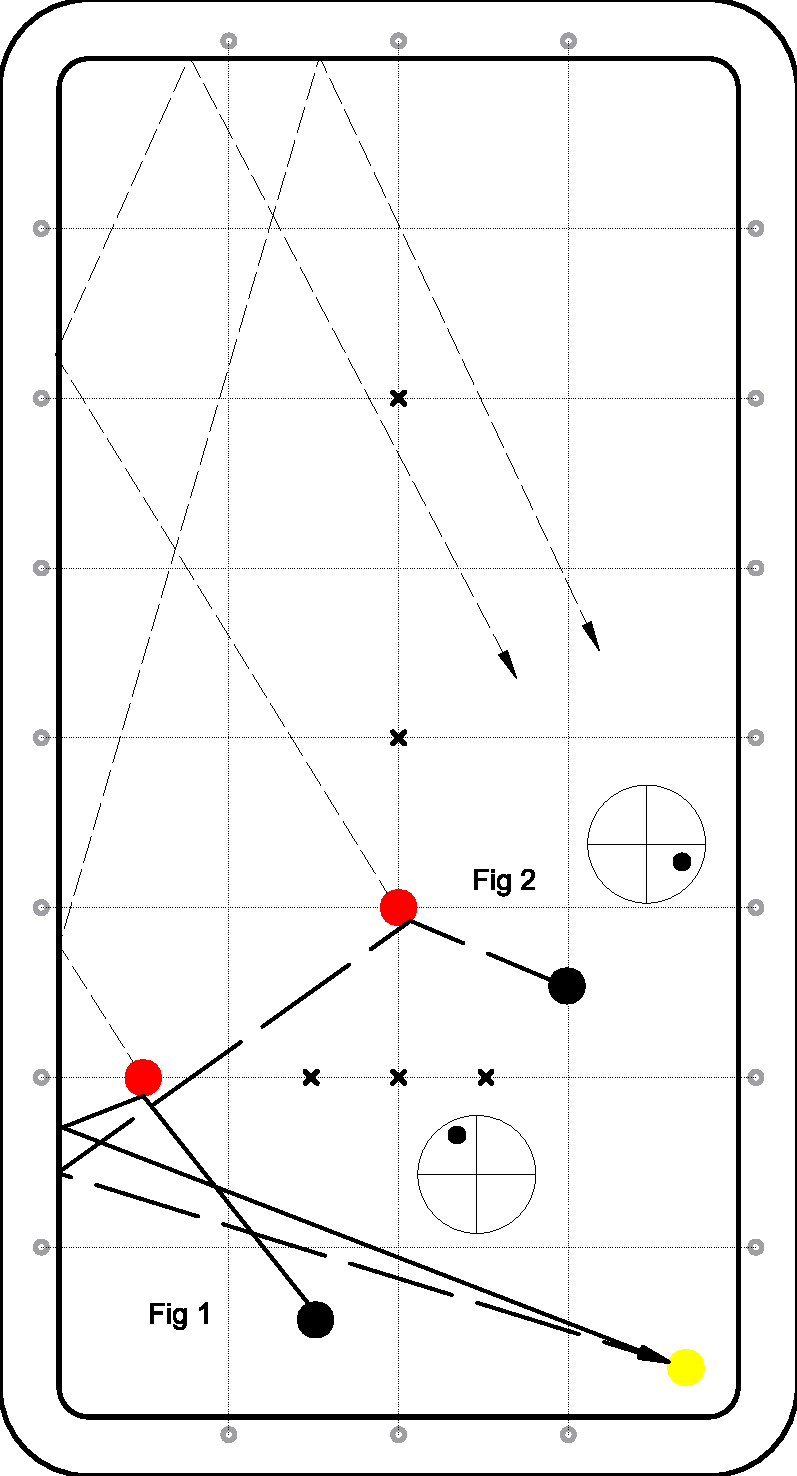
\includegraphics[width=0.85\linewidth]{B/imagesB/B07-01.pdf}
	\caption{ Rappels extr�mes par une bande}
	\label{fig:B07-1}
\end{figure}

\clearpage


% !TeX root = ../book.tex
% !TeX spellcheck = fr_FR
% !TeX encoding = ISO-8859-1

\section{Rappel � la petite bande}

Voil� encore un point qui se pr�sente tr�s fr�quemment. On peut aussi le
rencontrer le long de la petite bande ou bien dans le champ, la 3
n'�tant pas proche d'une bande.

Figure 1 : c'est le cas la plus courant. C'est un r�tro angle droit
appuy�, effet favorable. La 1 touche une bande ou parfois deux et la 2
se rappelle par trois bandes. Si l'inclinaison est trop faible sur la
grande bande de la direction 1-2, il sera peut-�tre pr�f�rable
d'attaquer la 2 plus grosse pour assurer sa rentr�e dans le chapeau. Il
conviendra alors de jouer un peu plus haut sur la 1 tout en restant sous
le milieu de la hauteur. Dans le m�me ordre d'id�e, si l'inclinaison 1-2
sur la grande bande semble trop imposante, il sera pr�f�rable d'attaquer
la 2 moins grosse avec une prise de la 1 un peu plus basse et �a,
toujours pour s'assurer la rentr�e au chapeau.

Figure 2 : L'inclinaison 1-2 sur la grande bande est faible et un 1B tel
que pour la figure 2 enverrait la 2 dans le coin oppos� loin de la 3 et
un r�tro direct ne permettrait pas un retour de la 2. On peut encore
tenter un 1B mais sans effet, voire effet contraire. La 2, faiblement
�cart�e de la grande bande, ne poss�de alors aucun effet qui
favoriserait son �loignement. La tentative avec effet contraire est
cependant assez difficile et une bonne habitude sera n�cessaire.

Remarques :

Plut�t que de risquer de voir la 3 � soulev�e � par la deuxi�me bande
de la 2, il sera souvent pr�f�rable de tenter un 1B sec qui �crasera la 3 sur la petite bande,
l'emp�chant de se sauver du chapeau. La 3 se trouvant dans le tiers
central de la petite bande, il conviendra avant l'essai, de bien estimer
le retour de la 2. Il serait dommage que le 2 rentre au coin derri�re le
jeu pendant que vous restez au milieu de la bande avec la 3. Enfin si la
taille du point d�passe un tiers de la table, la r�alisation devient
difficile et les retours plus al�atoires.

A l'entra�nement, il sera int�ressant d'essayer le bon effet, le sans
effet et l'effet contraire sans changer la position des billes au
d�part. Vous vous rendrez compte tr�s facilement des diff�rents
r�sultats et cela vous aidera dans vos choix futurs.

\begin{figure}[htb]
	\centering
	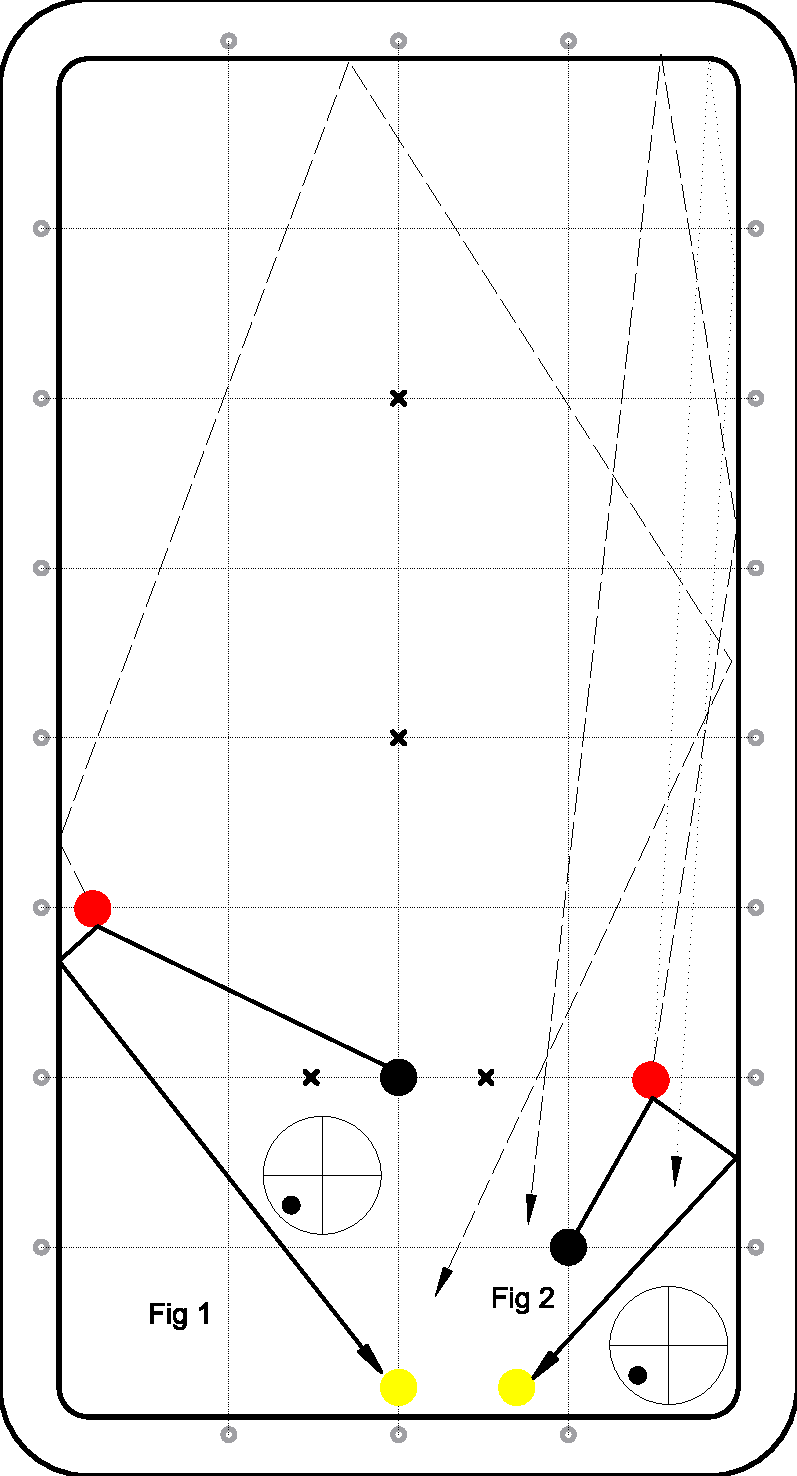
\includegraphics[width=0.85\linewidth]{B/imagesB/B08-01.pdf}
	\caption{Rappel � la petite bande}
	\label{fig:B08-1}
\end{figure}

\clearpage


% !TeX root = ../book.tex
% !TeX spellcheck = fr_FR
% !TeX encoding = ISO-8859-1

\section{Rappel direct ou par la bande ?}

Les joueurs voient en ce point, l'occasion d'une s�rie mais ils
n�gligent souvent la mani�re de le r�aliser. Comme le rappel est presque
une �vidence, le manque de pr�cision n'appara�t pas au premier coup
d'ail. Il conviendra non seulement de bien garder la 3 dans le coin mais
aussi d'y ramener la 2 dans le fameux chapeau.

Comme montr� sur la sous figure 1 de la \autoref{fig:B09-1}, il s'agit tr�s souvent d'un r�tro direct tout � fait normal. Nous aurons le soin de ne pas jouer trop loin du
centre bille tout en gardant la position r�tro. En approchant la fl�che
du centre et en laissant bien aller la canne avec le coup comme si on �
s'affaissait � dans la 2, la 1 revient doucement sans �clater la 2 au
retour et l'effet imprim� aide la 2 � � bien tourner �. Si l'angle form�
par la direction 1-2 et la grande bande proche emp�che la 2 de d'abord
toucher la petite bande oppos�e avant de revenir, la 2 ne reviendra pas
! D�s lors, il vaut mieux s'aider d'un r�tro bande afin de forcer le
toucher de la 2 sur cette petite bande quoique... si on s'en sent
capable, on peut encore jouer direct si la 2 touche la grande bande
oppos�e avant la petite bande mais pas trop loin du coin en prenant soin
de forcer le coup ; la 2 revient alors en �\textless{} cassant � le coin
avec son effet devenu contraire. (Ce rappel� est assez spectaculaire et
souvent appr�ci� du spectateur y voyant un coup contre nature...

\noindent Remarques :
\begin{itemize}
	\item Si le r�tro est un peu long, il faudra plus d'allonge, on jouera plus
bas et plus souplement.
\item Si le r�tro est court, relevez un peu la fl�che vers le centre bille
tout en restant dans la partie inf�rieure de la bille. Le r�tro court
permet un mouvement court de la 1 avec un mouvement long de la 2.
\item Si la 3 est proche de la petite bande et un peu �cart�e du coin, un deux
bandes sera parfois pr�f�rable. Si on a pris la 2 bien grosse et pas
trop bas, l'effet imprim� est d'une telle force qu'en touchant la petite
bande, la 1 reprend vigueur et se � couche � sur la petite bande.
\end{itemize}

Lorsqu'on sera bien habitu� � cette technique, on passera facilement �
celle de l'amorti qui permet d'encore mieux dominer le mouvement des
billes (4�ann�e).

Sous figure 2 de la \autoref{fig:B09-1} : L'angle form� par la direction 1-2 et la grande bande proche
est vraiment trop faible. Si le une bande bon ou mauvais effet n'est pas possible, la 2 s'�loignant trop
du coin o� rappeler, on peut encore appliquer un direct ... un peu
sp�cial... Il faut lever le talon avec la main arri�re jusqu'�
l'aisselle et plonger un ou deux millim�tres � l'ext�rieure de la 2, c�d
vers le milieu de la table avec un effet de l'autre c�t�. La 2 accentue
l'angle � la bande � cause du d�calage et la 1 effectue un arc de cercle
rentrant avant de toucher la 3. Difficile... � utiliser seulement si on
s'est bien habitu� � ce coup.

\begin{figure}[htb]
	\centering
	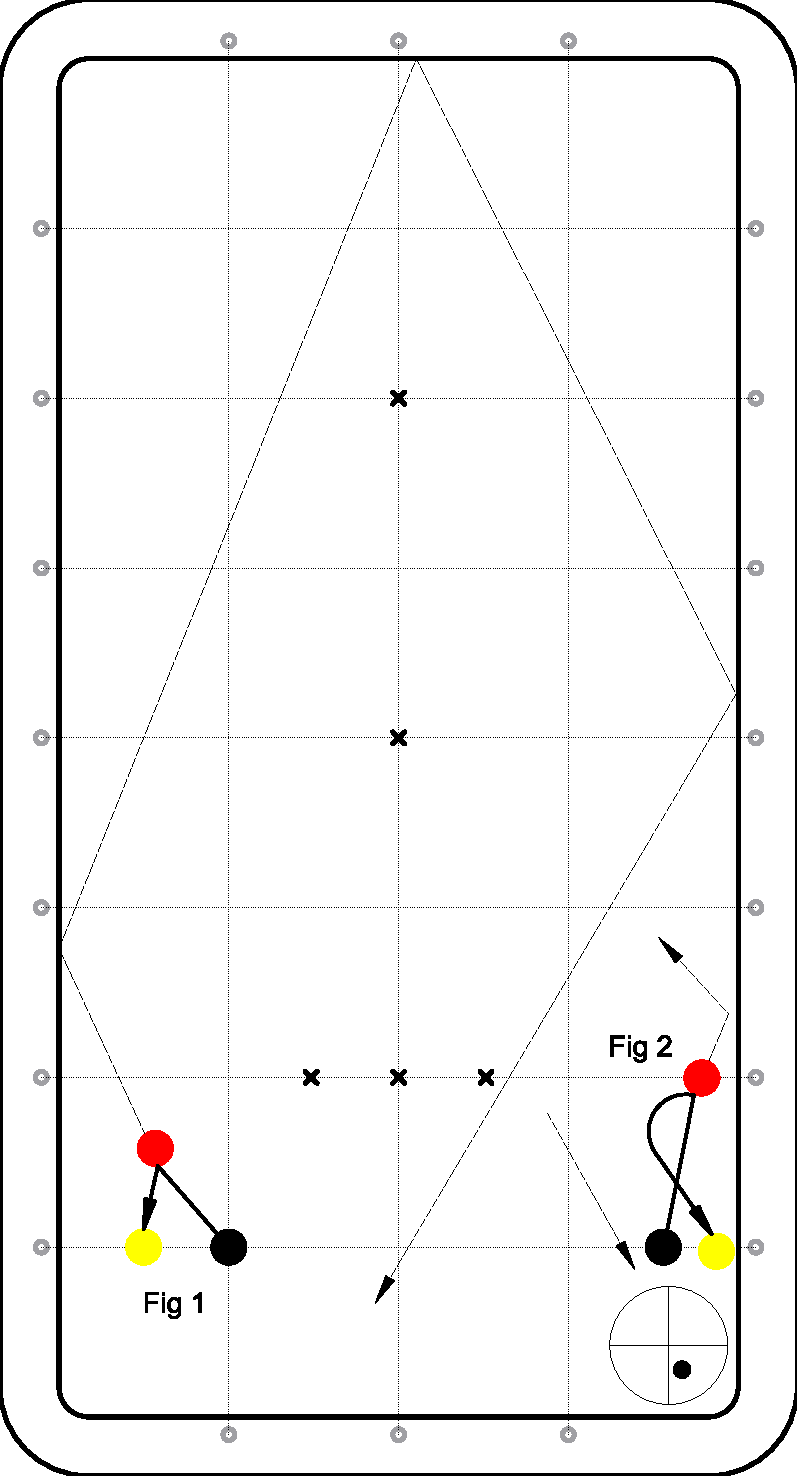
\includegraphics[width=0.85\linewidth]{B/imagesB/B09-01.pdf}
	\caption{Rappel direct ou par la bande ?}
	\label{fig:B09-1}
\end{figure}

\clearpage


% !TeX root = ../book.tex
% !TeX spellcheck = fr_FR
% !TeX encoding = ISO-8859-1

\section{Petit r�tro avec long d�placement}\label{sec:B10}

Ce point est assez difficile. Il demande une grande souplesse et une
bonne ma�trise du r�tro. Il conviendra de bien s'entra�ner sur cette
figure afin de gagner en confiance et de sentir d�j� les trois billes
dans le coin avant de jouer.

Comme le montre la figure, notre position au � milieu du jeu de quilles
� est tr�s inconfortable. Seule la bille 3 occupe une position
favorable. N'allons pas trop vite. Examinons bien avant de prendre notre
d�cision. Remarquons que la direction 1-2 coupe le haut de la table aux
environs du coin diam�tralement oppos� � la 3, disons dans le carr� du
coin : nous sommes sauv�. Appliquons un r�tro direct, petite fl�che,
main arri�re loin sur la canne, coup tr�s souple et pas trop fort, effet
� droite avec tenue l�g�re. Si la 2 touche la petite bande du haut,
l'effet favorisera sa rentr�e, si elle touche la grande, l'effet
retiendra son �cartement. Dans les deux cas, la 2 rentrera dans le coin
de la 3.

Deuxi�me solution : un 1B via la grande bande � notre gauche (en
pointill� sur la figure) est possible. Il s'agit d'un angle de 80�
environ, petite fl�che, main arri�re loin sur la canne, effet � gauche
bas de bille, coup souple et pas trop fort. Cette solution est plus
rassurante mais plus difficile. Elle demande une grande souplesse et la
grosseur de la prise sera fonction de la direction � donner � la 2 afin
qu'elle rentre au coin de la 3.

Remarques :

\begin{itemize}
	\item si la position est favorable, donnez la pr�f�rence au r�tro. C'est le
		meilleur moyen de ma�triser les billes .... � condition de bien
		ma�triser le r�tro !
	\item si la direction 1-2 coupe la petite bande oppos�e un peu loin du coin, 30, 40 cm, tentez le 1B souple.
	\item si la direction 1-2 coupe la petite bande ou la grande trop loin du
		coin, choisissez une autre solution car le rappel deviendrait vite
		impossible
\end{itemize}


\begin{figure}[htb]
	\centering
	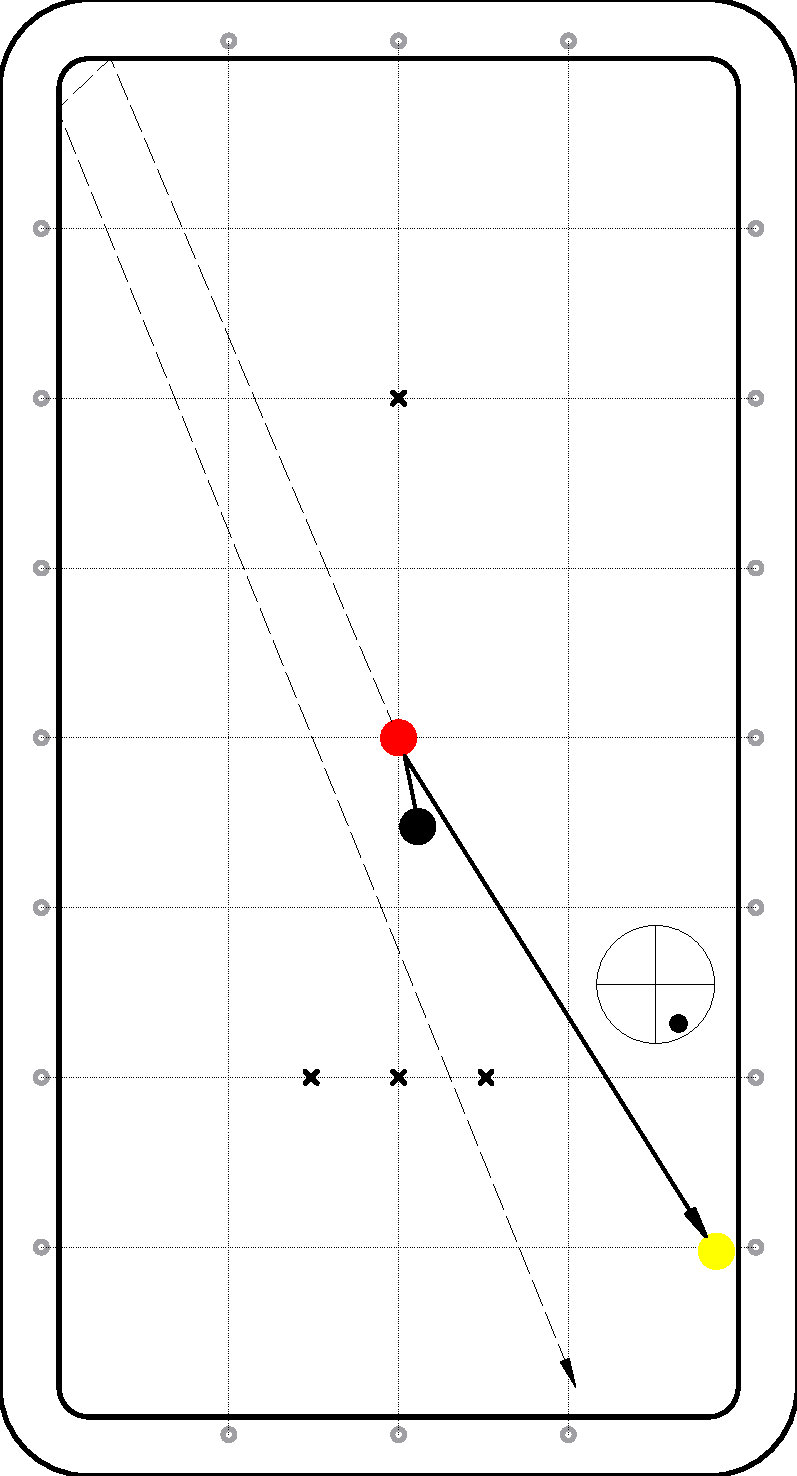
\includegraphics[width=0.85\linewidth]{B/imagesB/B10-01.pdf}
	\caption{Petit r�tro avec long d�placement}
	\label{fig:B10-1}
\end{figure}

\clearpage


% !TeX root = ../book.tex
% !TeX spellcheck = fr_FR
% !TeX encoding = ISO-8859-1

\section{}


\begin{figure}[htb]
	\centering
	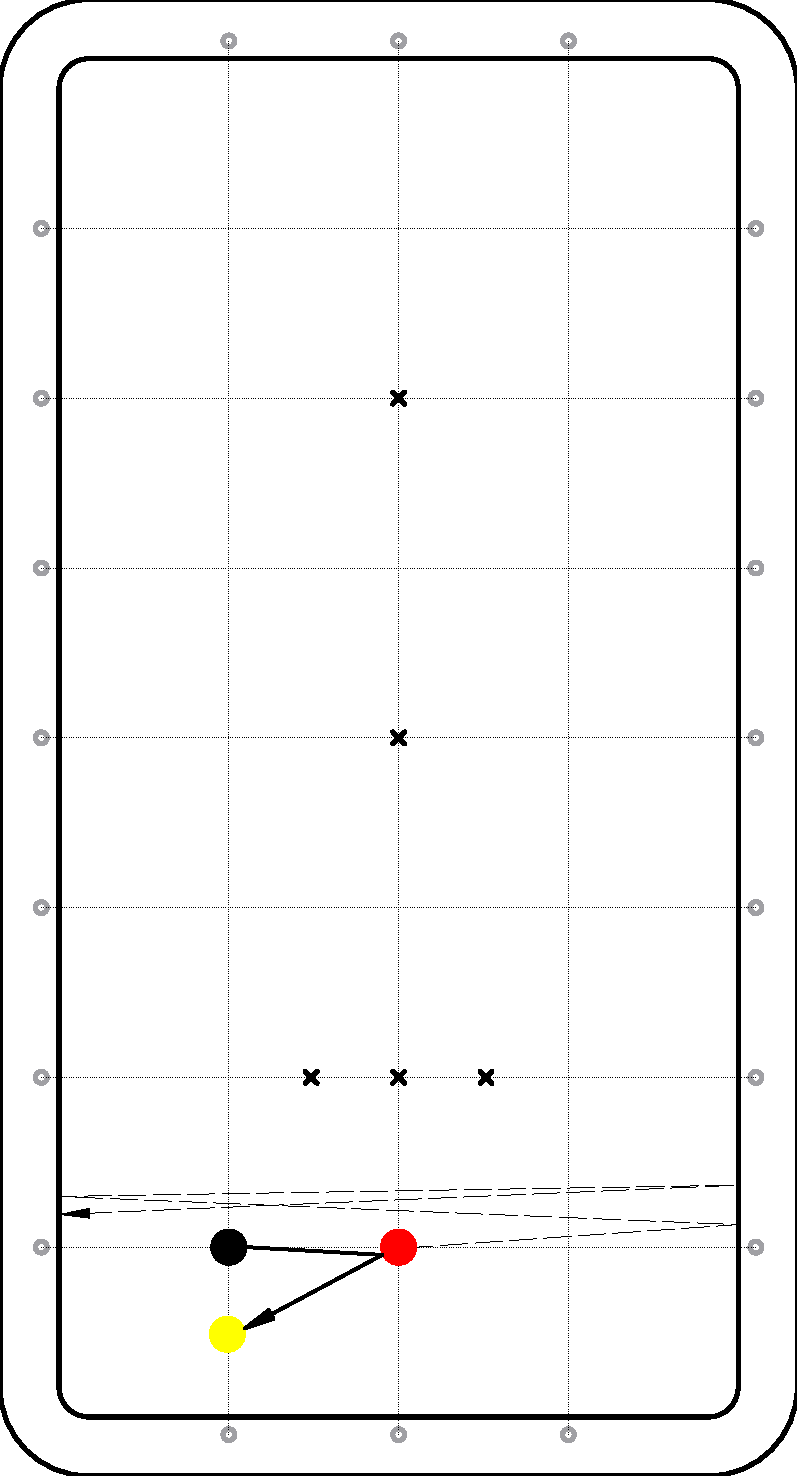
\includegraphics[width=0.85\linewidth]{B/imagesB/B11-01.pdf}
	\caption{}
	\label{fig:B11-1}
\end{figure}

\clearpage


% !TeX root = ../book.tex
% !TeX spellcheck = fr_FR
% !TeX encoding = ISO-8859-1

\section{}


\begin{figure}[htb]
	\centering
	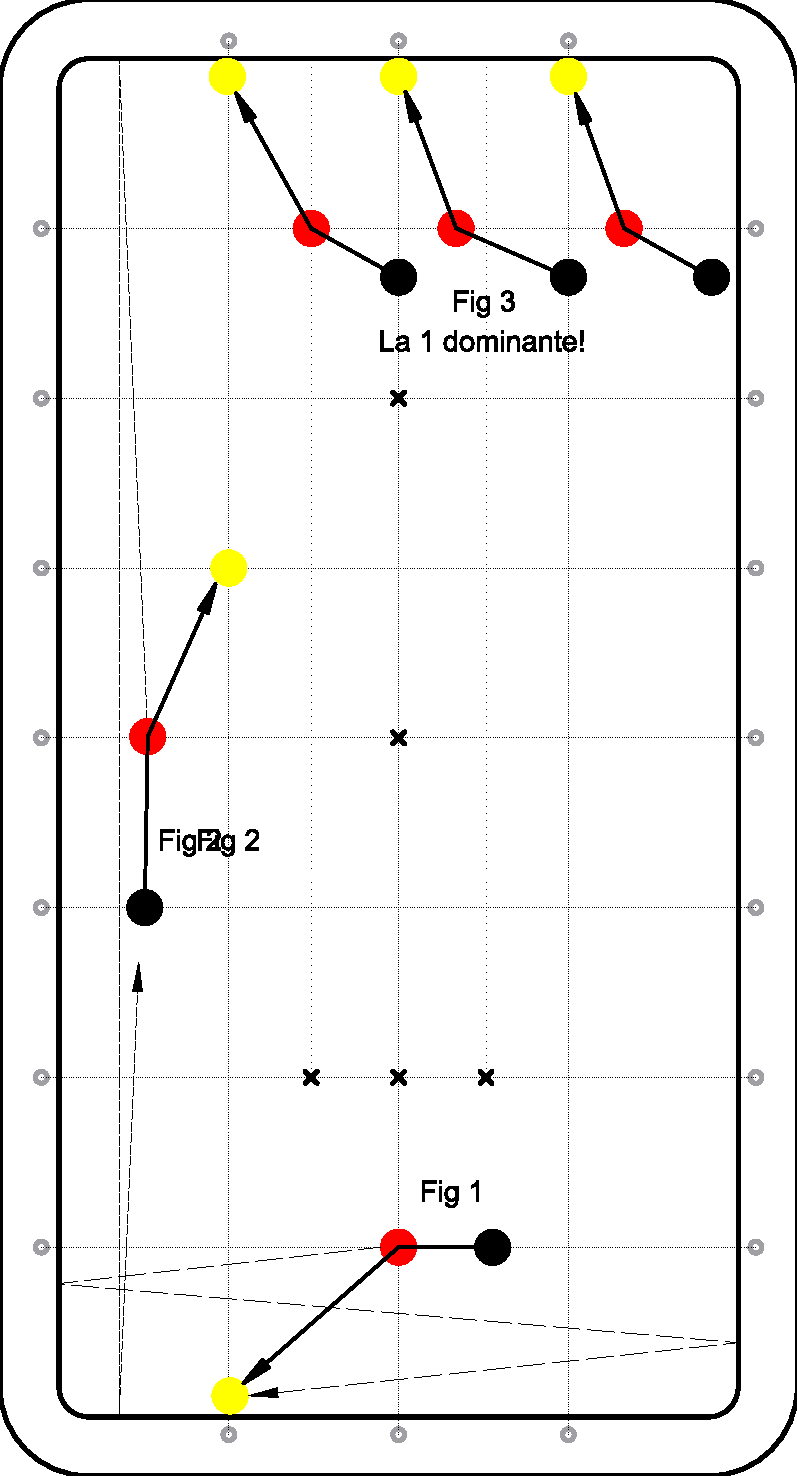
\includegraphics[width=0.85\linewidth]{B/imagesB/B12-01.pdf}
	\caption{}
	\label{fig:B12-1}
\end{figure}

\clearpage


% !TeX root = ../book.tex
% !TeX spellcheck = fr_FR
% !TeX encoding = ISO-8859-1

\section{La bricole simple}\label{sec:B13}

La bricole, m�me simple est un point angoisse FL pour beaucoup de
joueurs. Cependant le calcul est facile m�me si la figure para�t
compliqu�e.

Figure 1 : Les billes sont � peu pr�s � la m�me distance de la bande
choisie pour tenter le coup, une finesse �tant trop difficile ou
impossible. Par le centre de la 1, abaisser une perpendiculaire sur la
bande face aux billes 2 et 3, la coupant au point A. Du milieu du
segment 2-3, abaisser une perpendiculaire sur la m�me bande la coupant
au point B. Le milieu du segment A-B, soit le point R, -

constitue le point de rep�re rapproch�, soit le point R. Il ne nous
reste plus qu'� viser ce point sans effet R* et de pr�f�rence bille
en-t�te pour pallier � une e �ventuelle mini erreur de prise sans effet.

Figure 2 : Ce serait trop beau si les bricoles � r�aliser �taient
toujours aussi bien dispos�es. Ici, la 1 n'est pas � la m�me distance
que les billes 2 et 3. Il conviendra donc d'appliquer une correction au
calcul. Proc�dons d'abord comme expliqu� pour la figure 1. Abaissons les
perpendiculaires pour d�terminer les points A, B et R. Si nous visons ce
rep�re R, nous obtiendrions une trajectoire erron�e soit la droite �x�.
Tra�ons une parall�le � la grande bande passant par les centres des
billes 2 et 3 coupant la droite x en un point soit E. Abaissons la
perpendiculaire du point E vers la bande soit le point d'intersection C.
On a ainsi report� sur la bande, l'erreur commise par notre construction
initiale. Le milieu du segment R-C devient notre point de rep�re
rapproch� Rc (rep�re corrig�).

Remarque : L'habilet� du bricoleur consiste � bien fixer le point de
rep�re � viser. Comme il n'est pas autoris� d'utiliser les r�gles et les
�querres, outils bien utiles en l'occurrence, la r�ussite r�side dans la
facult� d'imaginer dans l'espace le trac� expliqu� plus haut. Il ne faut
pas h�siter � utiliser sa canne afin de projeter des directions
imaginaires seulement per�ues par le jo verra que des arabesques et
autres d�monstrations spectaculaires mais nous, on s'en fiche ! La
figure 2 comprend plus d'�l�ments que ceux r�ellement utilis�s, ceci
afin de montrer une construction compl�te pour les g�om�tres exigeants.
La r�alisation � sur le terrain � est plus ais�e que sur le papier.
Quand on aura acquis un peu d'habitude � l'entra�nement, on pourra
ais�ment se passer des interm�diaires. On se placera � la bande face aux
billes pour en appr�cier directement l'emplacement du point de rep�re
rapproch� m�me avec correction incorpor�e. Enfin, si les billes 2 et 3
sont un peu �cart�es ou inclin�es, c'est au joueur d'appr�cier l'endroit
o� il doit toucher pour r�aliser et par l� faire varier l'emplacement du
rep�re.

\begin{figure}[htb]
	\centering
	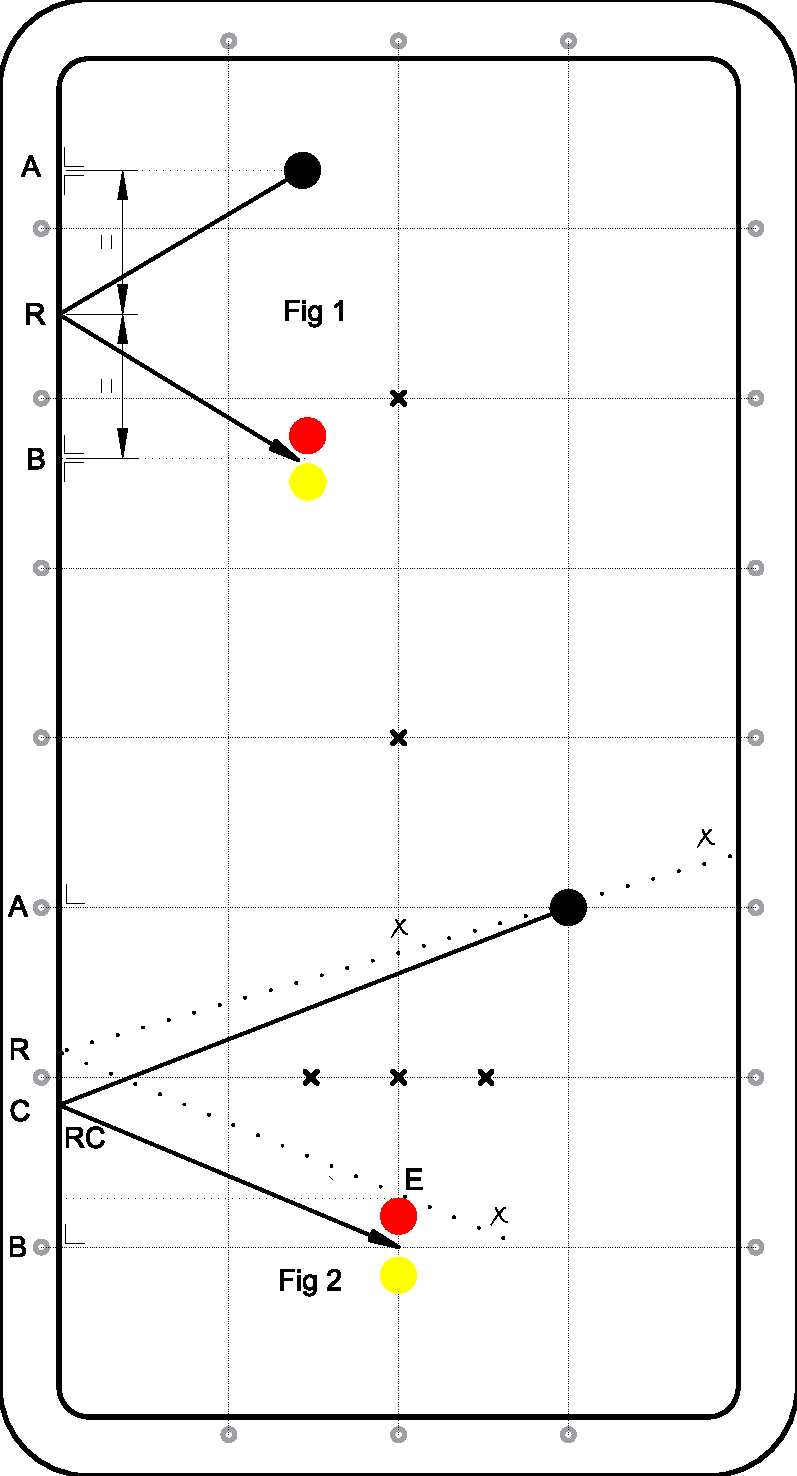
\includegraphics[width=0.85\linewidth]{B/imagesB/B13-01.pdf}
	\caption{La bricole simple}
	\label{fig:B13-1}
\end{figure}

\clearpage


% !TeX root = ../book.tex
% !TeX spellcheck = fr_FR
% !TeX encoding = ISO-8859-1

\section{}


\begin{figure}[htb]
	\centering
	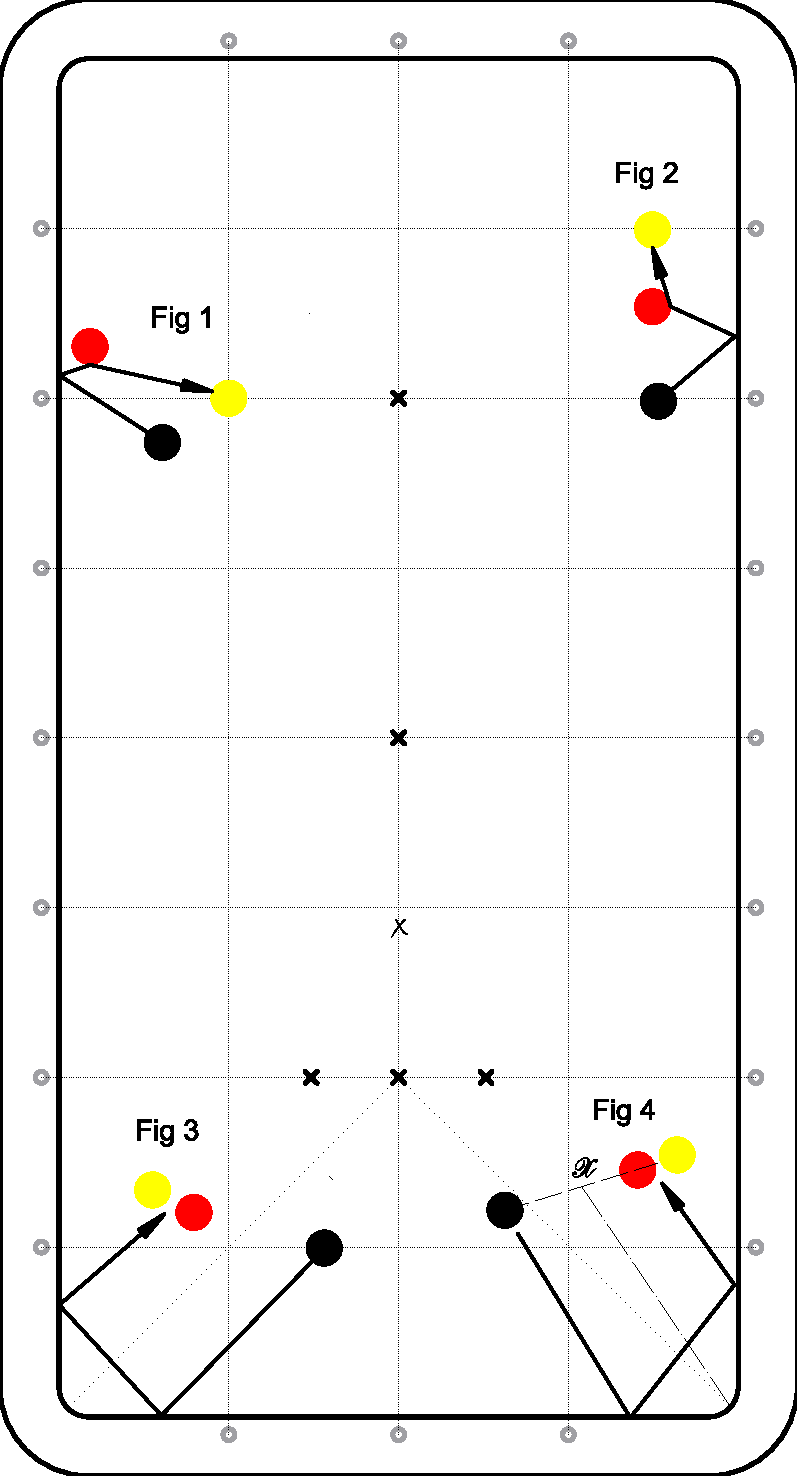
\includegraphics[width=0.85\linewidth]{B/imagesB/B14-01.pdf}
	\caption{}
	\label{fig:B14-1}
\end{figure}

\clearpage


% !TeX root = ../book.tex
% !TeX spellcheck = fr_FR
% !TeX encoding = ISO-8859-1

\section{Bricoles deux et trois bandes}\label{sec:B15}

Ce sont deux bricoles diff�rentes mais bien utiles et si souvent
n�glig�es au profit d'un 1B qui laisse la 1 au milieu des deux autres
billes.

Figure 1 : On s'est emp�tr� � la petite bande en tentant de rentrer les
billes 2 et 3. Un petit 1B ne serait pas une mauvaise solution mais elle
impose de nouveau un r�tro 1B � suivre et laisse la 1 avec une prise de
dominante difficile. Tentez donc une bricole 2B comme dessin� bille en
t�te sans effet et viser pour toucher la 2�bande juste devant la 2. La 1
aura tendance � prendre la dominante en un seul coup. Si par malheur ce
n'est pas parfaitement r�ussi, la situation ne sera pas d�t�rior�e par
rapport � la situation pr�c�dente.

Figure 2 : La position de la 3 est telle que son rappel est tr�s
difficile voire impossible. Un 1B sur la 3 donne un r�sultat tr�s
al�atoire. On devrait jouer assez fort et la 3 reviendrait au coin
pendant que la 2 change de c�t�. Un 1B sur la 2 est sans doute le point
le plus facile mais il donne une position tr�s inconfortable. Serrez
donc en un coup. Si la 2 n'est pas trop �loign�e de la petite bande,
appliquez une bricole deux bandes par l'arri�re, mi-hauteur ou mi-haute,
assez grosse et bon effet bien dos�. Les billes se retrouvent dans le
chapeau au croisillon du cadre. Au deuxi�me coup, vous aurez l'embarras
du choix pour � tourner � le jeu.

Remarques :
\begin{itemize}
	\item Une prise fine am�ne la 1 entre la petite bande et la bissectrice.
	\item Une prise moyenne am�ne vers la bissectrice.
\end{itemize}

Une prise grosse am�ne aussi vers la bissectrice avec une tendance � la
d�passer mais attention : pas beaucoup. Pour ramener la 1 plus pr�s de
la grande bande, il conviendra de bricoler bille basse avec un bon effet
maximum, presque coup du r�tro... - Le point est plus facile lorsque la
3 est un peu plus pr�s de la petite bande que la grande...

Notez bien : quel que soit l'essai, la position suivante sera presque
toujours favorable au jeu constructif. Ceci est un point typique du jeu
de cadre. Il demande une petite habitude pour jauger de la grosseur de
bille et l'�vitement de la bosse (pas toujours d�favorable) de la 1 sur
la 2 apr�s 3 bandes...


\begin{figure}[htb]
	\centering
	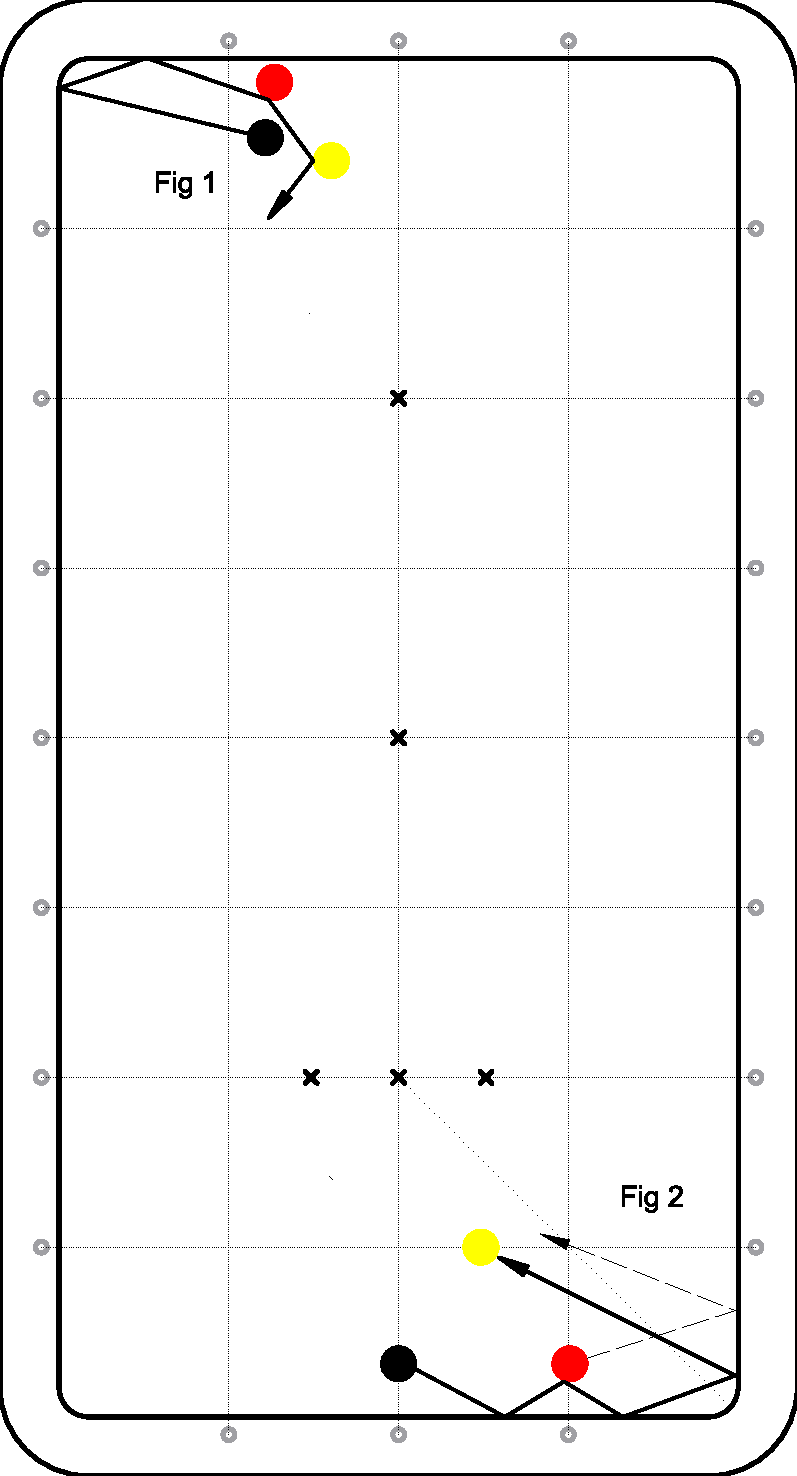
\includegraphics[width=0.85\linewidth]{B/imagesB/B15-01.pdf}
	\caption{Bricoles deux et trois bandes.}
	\label{fig:B15-1}
\end{figure}

\clearpage


% !TeX root = ../book.tex
% !TeX spellcheck = fr_FR
% !TeX encoding = ISO-8859-1

\section{R�tro deux bandes}\label{sec:B16}

Le r�tro deux bandes peut sauver des situations qui se d�gradent.

Comme le montre la figure, la 1 est face au coin et le jeu est en
expansion, c�d qu'il s'�loigne vers le milieu de la table. Aucun r�tro
direct n'assure une rentr�e convenable.

Dans certains cas un 1B sans effet vers la grande bande voisine peut
assurer une rentr�e de la 2 mais le coup est assez d�licat avec ce que
nous sommes suppos�s d�j� ma�triser. Nous le garderons en m�moire pour
l'appliquer �ventuellement plus tard.

L'exercice du jour consiste � s'habituer � appliquer un r�tro 2 bandes,
bille basse, assez grosse, effet favorable. La principale difficult�
r�side dans le choix du point de rep�re rapproch� sur la petite bande.
D'une mani�re g�n�rale, prenons l'habitude de l'�valuer au tiers de la
distance 3-grande bande � abaisser sur la petite bande lorsque les
billes 2 et 3 sont � peu de chose pr�s � la m�me distance de cette
petite bande et que nous tentons un r�tro � normal �. La bonne
estimation du point d'impact de la 1 sur la petite bande est important.
La bille poss�de un effet important qui rend l'angle de r�flexion assez
�vas�. Il sera prudent de tester avant de consommer ! Les tables et les
tapis poss�dent des � rendus � diff�rents. D�s que nous avons bien
rep�r� le point d'impact de la 1 � la petite bande, dans notre t�te,
nous avons transform� un 2B en un 1B ! Si les billes 2 et 3 ne sont pas
parall�les � la petite bande, il faudra bien estimer le point de rep�re
rapproch�, � l'?il. Enfin, ce point de rappel donne rarement un serrage
et encore moins souvent une position dominante mais il ne d�grade pas la
situation et permet souvent un positionnement favorable � la
construction.

\noindent Remarques :
\begin{itemize}
	\item le m�me point est jouable sur la grande bande, donc sur le c�t�.
	\item Un deux bandes peut �tre appliqu� � � l'envers � c�d sur la 3 vers la
	grande bande oppos�e. Essayez-le comme dessert. Il est moins difficile
	qu'il y para�t et il rentre la 3. (voir en pointill� sur la figure).	
\end{itemize}


\begin{figure}[htb]
	\centering
	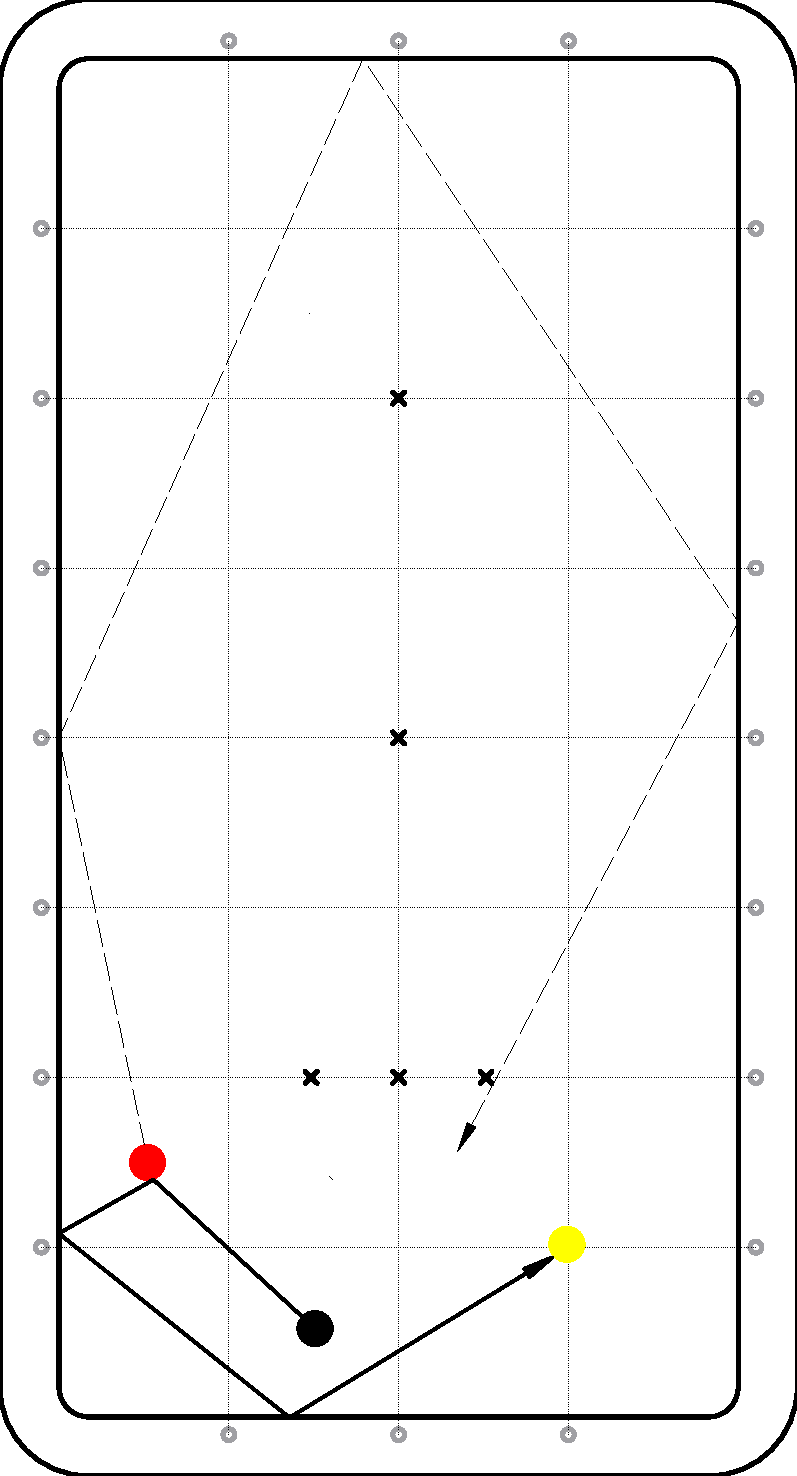
\includegraphics[width=0.85\linewidth]{B/imagesB/B16-01.pdf}
	\caption{R�tro deux bandes.}
	\label{fig:B16-1}
\end{figure}

\clearpage


% !TeX root = ../book.tex
% !TeX spellcheck = fr_FR
% !TeX encoding = ISO-8859-1

\section{}


\begin{figure}[htb]
	\centering
	\includegraphics[width=0.85\linewidth]{B/imagesB/B17-01.pdf}
	\caption{}
	\label{fig:B17-1}
\end{figure}

\clearpage


% !TeX root = ../book.tex
% !TeX spellcheck = fr_FR
% !TeX encoding = ISO-8859-1

\section{Rappel par le 8}\label{sec:B18}

Le rappel par le 8 est une appellation amusante inspir�e du dessin que
tracent les billes 1 et 2. Ce point est tr�s spectaculaire et il attire
l'admiration du spectateur. Jou� fort, avec les billes qui roulent et
voil� la 2 qui rentre doucement : �a �pate. Cependant, le coup est d'une
difficult� tr�s moyenne pour qui s'est un peu entra�n�.

C'est un r�tro violent, effet contraire et tr�s soutenu. La 1 revient �
petite vitesse sur la grande bande arri�re. Elle reprend vigueur � son
contact gr�ce � son effet puissant et assure tranquillement le chemin �
parcourir en une ou deux bandes jusqu'� la 3. Quant � la 2, son
cheminement para�t curieux bien que logique. Suivant le positionnement
1-2, elle sera projet�e violemment sur la grande bande oppos�e entre les
mouches 1 et 3, soit � peu pr�s � une distance de 30 � 90 cm du coin
sup�rieur, soit le point d'impact 11. Vu l'effet contraire induit, sa
course se redresse c�d qu'elle se rapproche de la perpendiculaire � la
grande bande en 11. Elle coupe la petite bande au point 12. Si on a
frapp� fort assez, elle conserve encore de l'effet contraire � ce moment
mais va le perdre apr�s l'impact sur la grande bande soit 13. La voil�
nantie d'un nouvel effet qui devient contraire en retrouvant la premi�re
grande bande, faible il est vrai, mais suffisant pour un dernier
redressement vers le chapeau.

\noindent Remarques :
\begin{itemize}
	\item Avant de tenter l'essai, on v�rifiera que le point 12 est bien situ�
	sur la petite bande moiti� gauche comme la figure le montre (moiti�
	droite si les billes sont plac�es de l'autre c�t�). Si jamais le point
	12 devait �tre situ� sur la grande bande, la 2 ne reviendrait jamais !
	\item Il est difficile d'amener les 3 billes dans le chapeau � chaque coup
	mais la nouvelle position gagn�e sera toujours plus favorable que la
	pr�c�dente.
\end{itemize}

Entra�nement: Exercez-vous � placer les billes 1 et 2 � diff�rentes
hauteurs, en restant de pr�f�rence dans la moiti� inf�rieure de la table
avec diff�rentes inclinaisons. Cela vous habituera non seulement � la
justesse du coup mais aussi � juger des fronti�res � ne pas d�passer.
Enfin, on peut aussi monter les billes 1 et 2 au-dessus du milieu de la
table mais la rentr�e deviendra de plus en plus difficile au fur et �
mesure que vous vous approchez de la petite bande sup�rieure. Vous
trouverez cet entra�nement instructif et divertissant.

\begin{figure}[htb]
	\centering
	\includegraphics[width=0.85\linewidth]{B/imagesB/B18-01.pdf}
	\caption{Rappel par le 8.}
	\label{fig:B18-1}
\end{figure}

\clearpage


% !TeX root = ../book.tex
% !TeX spellcheck = fr_FR
% !TeX encoding = ISO-8859-1

\section{Rappel par r�tro amorti}\label{sec:B19}

Voici deux exemples d'amortis avec les deux plaquettes B19 et B20. C'est
un avant-go�t de ce qui vous attend en quatri�me ann�e.

Figure 1 : Nous avons vu en premi�re ann�e, les points de vis�e qui
peuvent �tre pr�cis�ment d�termin�s sur la bille 1. Une bille fait un
peu plus de 6 cm. de diam�tre. Pour que la fl�che ne glisse pas, nous
sommes amen�s � la frapper dans un cercle inscrit au centre bille de
environ 3 cm. de diam�tre. Imaginez un cercle au centre bille de
seulement 1 cm de diam�tre. Ramenez mentalement tous les points de
vis�es d�j� connus vers le centre bille en suivant les rayons par
lesquels ils passent et arr�tez ces points d�s qu'ils sont dans ce
fameux cercle de 1 cm de diam�tre. Les points de vis�es dessinent la
m�me figure mais celle-ci est plus petite. Vous avez maintenant de quoi
jouer droit, coul� ou r�tro de la m�me fa�on mais pour r�colter les
m�mes r�sultats, vous devrez jouer plus gros, plus souple, plus fluide,
sans �-coup. Vous devrez p�n�trer (!) au lieu de frapper. La 2 aura une
direction plus proche de celle de la 1 dans son premier tron�on, qui,
elle, aura un mouvement plus lent car la 2 aura r�colt� la grosse part
de l'�nergie donn�e. Enfin la 2, avec une d�viation moins grande, moins
�clat�e, � rentrera � des positions jusqu'ici �incontr�lables �,

Figure 2 : C'est un angle droit inclin� � 45�. L'ex�cution d'un r�tro
habituel tel que nous l'avons vu, ram�nerait la 2 au mieux, au milieu de
la petite bande pendant que la 1 et la 3 seraient � la grande bande.
Prenez donc la 2 pleine moins un petit morceau (un ch�che) et visez,
comme pour un angle droit, le centre du secteur gauche inf�rieur,
attention, celui dans le cercle de 1 cm. au centre bille. Si vous
parvenez � bien vous abandonner dans votre acte, faisant confiance �
votre mat�riel, c�d en ne for�ant pas votre volont� de domination dans
votre coup, vous serez �tonn� du r�sultat, d'autant plus que cela aide �
la concentration et que vous allez avoir l'impression que vous et votre
canne ne faites plus qu'un ! Vous aurez l'impression que vous avez
acquis le pouvoir de d�cider que les billes se positionnent l� o� vous
d�sirez qu'elles soient. C'est grisant !

Remarque : L'abandon de soi est chose difficile. C'est une abn�gation de
sa propre personne. C'est faire confiance sans que nous ne puissions
intervenir m�me si nous savons que c'est nous qui l'avons produit. C'est
� ne rien mettre dans sa canne �. Ne mettre aucune intention, faire le
vide, ... ou toute autre expression d�crivant un �tat de d�pendance nous
est naturellement insupportable. Nous nous sentons � la merci du premier
venu... Pourtant, d�sol� pour les joueurs qui n'accepteront pas ou qui
ne parviendront pas � l'accepter, il n'y aura pas d'acc�s aux cat�gories
sup�rieures pour les rebelles...


\begin{figure}[htb]
	\centering
	\includegraphics[width=0.85\linewidth]{B/imagesB/B19-01.pdf}
	\caption{Rappel par r�tro amorti.}
	\label{fig:B19-1}
\end{figure}

\clearpage


% !TeX root = ../book.tex
% !TeX spellcheck = fr_FR
% !TeX encoding = ISO-8859-1

\section{}


\begin{figure}[htb]
	\centering
	\includegraphics[width=0.85\linewidth]{B/imagesB/B20-01.pdf}
	\caption{}
	\label{fig:B20-1}
\end{figure}

\clearpage


% !TeX root = ../book.tex
% !TeX spellcheck = fr_FR
% !TeX encoding = ISO-8859-1

\section{Long r�tro, petit d�placement}\label{sec:B21}

Cette position fait partie des tentations dangereuses. Il serait si
rassurant de faire un petit direct et d'engranger d�j� un point. C'est
vrai, mais il est trompeur. L'angle 1-3-2 est �vas� et un simple direct
n'est pas si simple. Pour peu qu'on soit oblig� de forcer ou de tenter
un 90�, nous resterions avec un point d'attente, au mieux, un coup de
rappel qui nous laisserait encore au milieu de la table. Beaucoup de
joueurs tentent m�me un 1B en touchant d'abord la 3. Quel
d�sappointement lorsque leur bille rate l'arri�re de la 2, laissant de
surcro�t, une position dominante � l'adversaire.

Il est temps de commencer � penser tactique. * Pousser les billes devant
soi les r�v�le. C'est d�j� bien. Les pousser � la grande bande en plus,
c'est mieux.

Enfin les pousser � la petite bande tout en gardant la dominante c�d que
la 1 est plus pr�s du milieu de la table que la 2 et la 3 : c'est le
pied !

� partir de maintenant, ayons toujours en t�te qu'il faut ramener les
billes � une petite bande et prendre la dominante. C'est le secret des
commencements de s�rie. Nous ne pouvons pas d�j� pr�tendre serrer le jeu
tout le temps ni que chaque position le permet mais le fait d'y penser,
de chercher, d'essayer, vos s�ries vont commencer � grandir... sans
qu'on ne s'en aper�oive. Et ne pensez pas � ce que vous laissez �
l'adversaire : si vous �tes plus fort, avec ou sans � jeu �, vous
gagnerez plus souvent que vous ne perdrez... la r�ciproque �tant vraie.

La figure : fl�che un peu longue, canne l�g�re mais ferme, main arri�re
loin sur le talon et coup de r�tro pas trop bas et de force soutenue
mais sans violence, effet � gauche. La 1 revient en direct sur la 3
lentement pendant que la 2 fait le tour de la table. A notre bonne
surprise, nous avons pris la dominante. Avec un peu de chance, le jeu se
poursuit par un coul� direct ou un 1B par l'arri�re de la 3... et nous
voil� ramen�s � la petite bande tout en gardant la dominante. C'est
merveilleux.

\noindent Remarques :
\begin{itemize}
	\item La prise grosse ram�ne la 2 haut.
	\item La prise fine la ram�ne basse.
	\item Suivant l'inclinaison 1-2, l'effet � droite redresse la 2 mais �mousse
	son �nergie. Nous avons la main mise sur le chemin que va emprunter la
	2.
\end{itemize}

Il est pr�f�rable d'avoir la dominante m�me un peu difficile plut�t
qu'un serrage mal foutu !

\begin{figure}[htb]
	\centering
	\includegraphics[width=0.85\linewidth]{B/imagesB/B21-01.pdf}
	\caption{Long r�tro, petit d�placement.}
	\label{fig:B21-1}
\end{figure}

\clearpage


% !TeX root = ../book.tex
% !TeX spellcheck = fr_FR
% !TeX encoding = ISO-8859-1

\section{Rappel arri�re par deux bandes}\label{sec:B22}

Au d�but de cette ann�e, nous avons d�j� vu un deux bandes (B01).
Celui-ci fut expliqu� � force de constructions g�om�triques et il
semblait bien compliqu�. L'exp�rience nous a montr� que la r�alit� du
terrain �tait moins difficile que la compr�hension du dessin.

Nous voici avec le m�me deux bandes mais la 1 se trouve � l'int�rieur du
jeu c�d plus pr�s du coin envisag� pour le calcul que les deux autres
billes. Nous n'avons donc pas les billes devant la 1 et nous n'avons pas
la dominante. Nous sommes apparemment dans une position d�favorable, de
destruction...

Nous allons commencer par faire le m�me trac� g�om�trique que pour la
fiche B01. Appr�cions le milieu du segment 2-3, soit le point X. Tra�ons
mentalement une droite passant par X et le coin, soit la droite y.
Tra�ons une parall�le � cette droite passant par le centre de la 2 soit
z. Cette parall�le coupe la bande au point R qui devient notre point de
rep�re rapproch�. Il nous suffit maintenant de jouer un coup direct en
r�tro, effet favorable normal...2-R-3 ... Pas si vite ! Le calcul est
exact mais l'effet induit en bas de bille est trop puissant
naturellement et � notre d�sappointement, la 1 va passer en bas de la
3... Il sera donc indispensable d'appliquer une correction. Pour cela,
chacun a son truc... Je vous livre le mien quitte � choisir le v�tre
pourvu que �a marche. Cette parall�le qui d�termine le point R, avec la
bille 2 pour centre, je la fais pivoter vers le haut de la table, donc
en s'�loignant du coin, d'un angle d'environ 15�... d�terminant ainsi un
point de rep�re corrig�, soit Rc... Il nous reste � appliquer le r�tro
normal, d�j� cit� plus haut, consid�rant maintenant le point 2-Rc-3. Ne
jouez pas trop fort : juste pour faire le chemin.... La 2 va faire le
tour de la table et revenir gentiment dans le chapeau.

Remarque : Vous n'�tes pas tir� d'affaire car vous n'avez pas la
dominante mais le point est maintenant beaucoup plus facile et un jeu de
construction est envisageable. Celui qui ma�trise bien ce point a
l'avantage de r�duire les risques d'un jeu �clat�.

Entra�nement : Laissez la 3 comme sur la figure et faites varier la
hauteur de la 2 entre les mouches 1 et 3. Placez la 1 de mani�re � �tre
amen� � devoir ex�cuter un angle sup�rieur, puis �gal et enfin inf�rieur
� 90� en n'oubliant pas de prendre la 2 en r�tro m�me en finesse s'il le
faut. Quand vous parviendrez � 100\% de r�ussite, votre moyenne montera
au moins de 1. La joie...

\begin{figure}[htb]
	\centering
	\includegraphics[width=0.85\linewidth]{B/imagesB/B22-01.pdf}
	\caption{Rappel arri�re par deux bandes.}
	\label{fig:B22-1}
\end{figure}

\clearpage


% !TeX root = ../book.tex
% !TeX spellcheck = fr_FR
% !TeX encoding = ISO-8859-1

\section{Coul�s en Cascade}\label{sec:B23}

Le coul� en cascade n'est pas un point en soi mais une tactique, une
m�thode pour gagner le tiers du billard tout en gardant une position
dominante. Elle a pour but de ramener les billes pr�s de la petite bande
en les laissant group�es.

Voyez la figure : au d�part, nous sommes dans une position favorable de
construction mais au milieu du jeu de quilles. Examinez bien la
situation. Nous avons l'embarras du choix quant � la mani�re de jouer :
\begin{itemize}
	\item Tenter une finesse assure le point mais nous place non seulement au
	milieu des deux autres billes mais encore nous laisse au milieu de la
	table. Avec de la chance nous serons peut-�tre bien plac�s pour op�rer
	un r�tro r�parateur et r�cup�rer la dominante que nous aurons perdu :
	en g�n�ral, ce sera une mauvaise solution.
	\item Si nous la � voyons �, nous pouvons faire un r�tro sur la 3. Nous
	prenons la dominante de l'autre c�t� de la table mais le serrage du
	jeu est loin d'�tre assur�. Cette solution est donc meilleure mais
	perfectible.
\end{itemize}

Un coul� est tellement plus prometteur... Position 1-2-3: Appliquez un
coul� simple. Evidemment, le jeu ne se serre pas d'un coup mais pour peu
qu'on ma�trise bien sa force et sa pr�cision, l'ensemble se rapproche de
la petite bande et nous restons en dominante. Position 1'-2'-3',
r�sultat du coup pr�c�dent : re-coul� qui nous rapproche encore du fond
de la table en faisant tourner l�g�rement la figure. Position 1"-2"-3" :
c'est le coul� auquel on r�ve, celui qui regroupe, qui serre. On profite
m�me du barrage pr�s de la petite bande. C'est une promesse de s�rie qui
s'annonce.

Remarque : Expliqu� de la sorte, nous sommes dans le r�ve, dans l'id�al.
La r�alit� sera souvent plus prosa�que et la dentelle figur�e moins
r�guli�re. On devra parfois jouer plus dur, ou plus amorti ou m�me
transformer un coul� en r�tro. Il conviendra de bien choisir � chaque
�tape. L'important est de garder le principe en t�te.

Entra�nement : Placer les billes en position de construction comme le
montre la figure et essayer d'ex�cuter la cascade jusqu'� ce que le
raisonnement sur papier devienne une m�canique dans les mains. Ce sera
gagn� lorsque vous parviendrez � amener les 3 billes � la petite bande
dans un chapeau tout en gardant la dominante. Bon courage...


\begin{figure}[htb]
	\centering
	\includegraphics[width=0.85\linewidth]{B/imagesB/B23-01.pdf}
	\caption{Coul�s en Cascade.}
	\label{fig:B23-1}
\end{figure}

\clearpage


% !TeX root = ../book.tex
% !TeX spellcheck = fr_FR
% !TeX encoding = ISO-8859-1

\section{}


\begin{figure}[htb]
	\centering
	\includegraphics[width=0.85\linewidth]{B/imagesB/B24-01.pdf}
	\caption{}
	\label{fig:B24-1}
\end{figure}

\clearpage


\chapter{La queue lev�e}

% !TeX root = ../book.tex
% !TeX spellcheck = fr_FR
% !TeX encoding = ISO-8859-1

\section{Piqu� de base et position du tr�pied}\label{sec:C01}

Cette troisi�me ann�e sera consacr�e aux � mains lev�es �... Ce sera
fatigant! Aussi, nous alternerons des s�ances plus reposantes. La
technique de l'ann�e pr�c�dente nous a d�j� amen� � un bon niveau de
connaissance. Celle-ci v? nous apprendre � conserver la main lorsque les
billes sont malheureusement masqu�es ou bien nous emp�chent de placer
correctement la main.

Les piqu�s (et les mass�s) constituent une famille d�licate o� la
position et la stabilit� de la main sont primordiales pour la pr�cision
du coup et la s�curit� du tapis. Comme le montre la figure, nous sommes
en pr�sence d'un r�tro mais la 3 nous emp�che de nous placer
correctement. Nous voil� oblig�s de jouer par-dessus. On prendra donc la
1 � en-t�te �, la canne s'approchant de la verticale, sans effet, droit
sur la 2. Un petit coup souple, charg� seulement du poids de la canne et
c'est r�ussi. Facile � dire.

Pour la main au tapis, nous adopterons la position du tr�pied. Nommons
les doigts de a,b,c,d et e en partant du petit doigt vers le pouce. Les
doigts a, b et c constituent les pieds du tr�pied. Disposons-les en
triangle, pointe au tapis, main dress�e, de mani�re � former une base
stable, Poussons l�g�rement sur les doigts afin d'assurer une bonne
assiette � l'�difice. Replions le doigt d afin qu'il ne g�ne pas le
mouvement. Levons le doigt e, le pouce, tendu et le plus haut possible,
toutefois sans se faire mal. Le plat de la main est tendu et fermement
stabilis�. Le pouce tendu fait appara�tre une petite pommette entre
lui-m�me et son voisin. A c�t� de cette pommette appara�t un petit
creux. La canne se posera sur le revers de la main et glissera dans ce
creux.

Pour la main lev�e : Le talon de la canne est soutenu entre le pouce et
l'index, sans forcer. Au moment du coup, la canne est accompagn�e par la
main sans donner plus de force que sa propre inertie. On peut dire que
la main lev�e dirige et maintient plus qu'elle ne joue. Le choc est
doux.

Remarque : Le piqu� se pr�sente comme un r�tro lev�. Qui dit r�tro, dit
prise en bas de bille. Exact ! Mais il convient d'appr�cier ce bas de
bille sur l'image que nous donne notre �il. Comme nous sommes � haut
>> devant notre bille, l'image qu'elle donne
est presque horizontale. Nous appr�cierons la partie basse comme �tant
celle la plus proche de notre corps. Pour un spectateur, il verra que
nous jouons haut... mais nous, nous savons que nous piquons dans le �
bas �.

ision du jeu n'est pas chose ais�e. Jamais notre vil ne sera en face du
jeu. On s'approchera de la v�rit� en plaquant notre ail le plus pr�s
possible de la canne lev�e. Enfin, toutes les mains ne sont pas les
m�mes et il faudra parfois composer...

Encore une fois : ne jamais forcer !

\section{Le piqu� le long d'une bande}\label{sec:C02}

Le piqu� le long d'une bande ne permet pas de placer facilement la main
d'assise correctement en position tr�pied. On d�posera donc cette main
sur la bande de la table mais dans une position de pr�f�rence moins
haute. Deux techniques de poses sont ici pr�sent�es :

Figure 1 : La main est pos�e comme pour le piqu� naturel mais les doigts
de base sont joints au lieu d'�tre �cart�s. Le tr�pied devient un �
unipied � � gros pied. Si on �cartait les doigts, la position
deviendrait tr�s pr�caire et vous auriez du mal � garder la fl�che dans
l'espace de jeu.

Figure 2 : Comme le rebord de la table est d�j� � une certaine hauteur
par rapport au plan de jeu, la position du tr�pied n'est pas
indispensable. En pliant la main � angle droit, tous les doigts sauf le
pouce, peuvent avoir deux phalanges dos � plat sur le rebord, le pouce
restant haut et arqu�. La main est pouss�e vers le bas afin d'assurer
une bonne stabilit� : c'est la position en �querre. La canne viendra se
poser sur le dos de la main, dans le creux pouce - pommette, comme pour
le piqu� naturel.

Remarque 1 : R�visons r�guli�rement notre facult� � plier la main. Tous
les joueurs n'ont pas les doigts d'�gale longueur. Souvent, il sera
n�cessaire de composer avec la th�orie. Comme la stabilit� de la main
est indispensable, on devra parfois sacrifier une phalange ou 2 voire un
doigt complet et g�nant.

Remarque 2 : Si la bille 1 touche ou bien se trouve tr�s pr�s de la
bande, on devra veiller � ce que le plan vertical d�termin� par la canne
et le sens du coup � porter ne coupe pas ladite bande, sinon il y a
queutage ! Pour bien juger, l'arbitre doit se placer en face du joueur
et regarder si la canne n'est pas inclin�e vers cette bande. C'est l�
aussi qu'on reconna�t les bons arbitres. C'est l� aussi qu'on reconna�t
les joueurs malicieux qui profitent de la na�vet� ou de l'ignorance de
leurs juges volontaires pour la corv�e... En effet, un bon queutage
assure le point et la rentr�e de la 2 � c�t� du paquet et non en ligne
droite. En cas de triche, c'est l'adversaire assis qui r�le et qui se
promet de s'y mettre �galement, ce qui est bien dommage pour le jeu de
billard.

Remarque 3 : Le piqu� le long d'une bande offre une position confortable
lorsqu'on est sur sa bonne main : le corps est bien d�gag� et le jeu en
face...

Si on est sur sa mauvaise main, le corps en g�ne la pose. Un droitier
posera sa fesse gauche sur le rebord de la table, la jambe gauche pli�e
et ballante, le pied sans appui, le pied droit, � plat au sol, assurant
la stabilit� du corps de mani�re � aligner celui-ci dans la vision du
jeu. Pour un gaucher, c'est la m�me chose � l'envers...

\section{Piquer sans queuter}\label{sec:C03}

Les piqu�s (et les mass�s) sont tr�s d�licats. Beaucoup de apparemment
queut�s ne le sont pas et beaucoup de apparemment propres le sont.
L'appr�ciation du queut� est autant difficile au joueur qu'� l'arbitre.
Aussi, voici quelques conseils au joueur afin de ne pas mettre l'arbitre
mal � l'aise et aussi quelques conseils de placement pour l'arbitre afin
qu'il puisse juger plus s�rement. La connaissance du point et des
positions � adopter est indispensable. C'est par l� que tous p�chent, �
tous niveaux, et il n'est pas rare que les esprits s'enflamment r�v�lant
au � connaisseur � la faiblesse de l'autre, mais comment le prouver si
l'autre ne sait pas et comment �tre s�r qu'on a raison ? Pour ma part,
lors d'une contestation, si je suis arbitre, je v�rifie que ma position
�tait correcte et propose m�me (vanit� personnelle), mon explication
apr�s le match, non pas ce qui s'est pass� mais ce que j'ai vu. (Il est
rare qu'un joueur d�sire cette explication mais cela arrive parfois). Si
je suis le joueur contestateur, je v�rifie que l'arbitre �tait bien
plac� pour juger. Si c'est le cas, je r�le probablement int�rieurement
mais je ne rousp�te pas. Si ce n'est pas le cas, je rousp�te et j'ai
tort... Comme dans tous les sports, rousp�ter ne fait jamais revenir
l'arbitre sur sa d�cision et on s'�nerve inutilement alt�rant la suite
de son jeu.

Prenez garde au piqu� : un vil vous regarde. D�fendez votre connaissance
et pas votre foi !

Figure 1 : Les billes 1 et 2 sont distantes d'au moins 6 cm. soit une
�paisseur de bille. A moins de glisser, il n'y a pas de danger de
queutage. La canne peut �tre inclin�e comme on le d�sire.

L'arbitre se met de c�t� pour v�rifier qu'on ne touche pas ou qu'on ne
glisse pas...

Figure 2 : Les billes 1 et 2 sont distantes de l� 2 cm. Le danger n'est
pas grand mais il faut rester prudent. Veillez � ce que, lorsque vous
prolongez l'image de la canne et de la 1 vers le tapis, cet espace ne
coupe pas l'image de la 2, d�s lors, il n'y a plus de danger m�me jou�
fort et m�me avec le � bruit � que certains brandissent comme preuve
unique de la faute. Ce fameux bruit ne vaut que lorsqu'il confirme ce
que l'eil a vu !

L'arbitre se met de c�t� et v�rifie que la position du joueur telle que
d�crite ci-dessus est correcte. Attention, la position pourrait �tre
incorrecte et le point valable si le joueur a jou� tr�s court. L'arbitre
devra donc v�rifier que la 1 ne � s'enfonce pas dans la 2 �.

Figure 3 : Les billes 1 et 2 sont distantes de 1 � 2 mm. Le danger est
grand. Le point de face est possible mais tr�s dangereux. Il serait
prudent d'appliquer un d�tach�, point que nous verrons plus tard. Pour
l'exercice, jouons de face avec la canne presque verticale.

L'arbitre se trouve de c�t� avec les m�mes r�gles que pour la figure 2.
Il doit s'attendre � un queut� et bien v�rifier que la 1 � enfonce � la
2 avant de sanctionner.

\section{Le piqu� angle droit}\label{sec:C04}

Une fois la position des mains bien assimil�es et la stabilit� de la
main au tapis assur�e, le piqu� devient un point relativement � facile
�. Au d�but on s'en �tonne toujours.

Figure 1 : il s'agit d'un angle droit. Le piqu� est int�ressant dans la
position propos�e car il permet de garder la dominante et la 2 n'ira pas
trop loin ce qui pourrait s'av�rer dommageable si on appliquait un
r�tro.\\
La part de bille � viser est un peu comme si la 2 collait � une bande,
comme dans le cas du point bosse, si vous vous souvenez bien, la 2
servant de miroir. Cela veut dire qu'on prendra de la bille 2, la moiti�
de ce qu'on prendrait si on appliquait un r�tro normal.\\
Ainsi pour l'angle droit, nous prendrons la moiti� de 3/4 soit 3/8 de
bille, une petite moiti�... Le mordant au tapis est suffisant pour une
courbure de 90�.

Attention ! Pas d'effet ! L'influence de l'effet, m�me faible, serait
surprenante. La canne doit �tre maintenue bien fixe dans sa direction.
La moindre d�viation de celle-ci imprimerait une courbure tr�s aigue.
Attention aussi � ne pas queuter ! La r�gle g�n�rale reste
d'application. Si les billes 1 et 2 sont assez proches, on veillera �
placer la canne de mani�re que son prolongement et l'image de la 1 ne
coupent pas l'image de la 2... sinon le point devra �tre annul� !
Beaucoup d'arbitres s'y laissent prendre. Jouant de c�t�, le coup porte
la confiance en lui. Pourtant, certains malins appliquent bel et bien un
petit queut� qui ne fait pas de bruit, donnant ainsi une impulsion
suffisante � la 2 pour la ramener � c�t� de la 3.

Remarque 1 : Ce queut� est faible et reste d�licat � sanctionner.
Cependant, le laisser passer n'avantagera peut-�tre pas ceux qui
l'appliquent sans le savoir mais ravira les sp�cialistes du genre, en
g�n�ral, des cat�gories sup�rieures dont le statut les met � l'abri des
sanctions d'arbitres moins forts qu'eux, donc h�sitants...au grand dam
de l'adversaire...

Remarque 2 : Je d�sirerais ici et en guise de dessert, revenir sur le
piqu� le long d'une bande. Voyez la figure 2. C'est le cas o� les billes
sont un peu �loign�es de la bande qu'elles c�toient mais pas
suffisamment pour glisser la main au tapis. Dans ce cas, on peut encore
placer les doigts sur le rebord de la table, bien arquer le pouce et �
tourner � la main de mani�re � amener la canne face aux billes. Cette
position ne peut s'obtenir que sur � sa bonne main �.

\section{Le r�tro fouett�}\label{sec:C05}

Apr�s avoir souffert des fiches \textless{}\textless{} bien remplies �,
nous allons un peu nous reposer avec quatre petites positions un peu
sp�ciales, ainsi le r�tro fouett� qui est un point interdit parce que
l'arbitrage en est tr�s difficile et qu'il suscita dans le pass�, des
disputes � vous fendre le cour.

Voyons la figure : les billes 1 et 2 sont tr�s proches l'une de l'autre,
de l'ordre du mm. Il suffit d'appliquer un r�tro direct et tout rentre
dans le chapeau ! Facile � dire. Le r�tro doit �tre tent� fort, bas,
tr�s bas, effet obligatoirement contraire, avec une canne l�g�re, sans
serrer, � peine tenue. De plus la direction de la canne ne peut pas
couper l'image de la 2 sinon ce sera compt� queut� donc faute ! Donnez
le coup en laissant travailler la canne d'elle-m�me, sans forcer.

M�me bien plac�, le queut� est dangereux. Si on a pris la bonne position
pour la canne et qu'on queute, la 1 est projet�e vers l'avant et le
point sera rat�. Si on ne queute pas, la 1 fait un bel arc de cercle
arri�re en acc�l�rant d'abord avant de stabiliser sa vitesse.

Le queut� est �vit� dans la mesure ou on n'a pas tenu sa canne au-del�
de la fronti�re de la 2. En effet, la canne ne touche jamais la 1 que
sur une courte distance quel que soit le coup. En laissant faire la
canne, en ne la maintenant pas, celle-ci s'arr�te au moindre choc. La 1
revient en arri�re en s'�cartant et ne retouche donc pas le proc�d�.
Bonne chance et surtout ... bon amusement.

Remarque : Ce point est interdit parce que trop difficile � juger. Il
est cependant int�ressant de le tenter � l'entra�nement parce qu'il est
un bon enseignement pour la souplesse et la connaissance du queut� mais
il ne sera �videmment pas tent� en comp�tition !

L'arbitre : tr�s int�ressant aussi pour s'habituer � juger le queut�.
L'arbitre doit se placer en face du joueur de mani�re � voir si la canne
ne coupe pas l'image de la 2 auquel cas il annoncera faute. Si la
position est correcte, il appr�ciera le mouvement de la 1 pour annoncer
faute ou non.

Remarque pour l'arbitrage : lorsque le joueur a rat� le point en
commettant une faute, il est utile que l'arbitre annonce faute d'abord
puis compte le score plut�t qu'annoncer seulement le nombre de points
r�alis�s avant d'inviter l'adversaire � la table. Par cette pratique il
fait savoir aux deux joueurs, qu'il a vu la faute, qu'il la conna�t. Les
joueurs sont pr�venus de la valeur de l'arbitre !

\section{Le r�tro masqu� }\label{sec:C06}

Le r�tro masqu� serait un r�tro � normal � si la 3 n'emp�chait pas de
placer correctement la canne. La bille 3 masque donc la vue et l'endroit
o� placer la main.

Adoptons la position de la main avant en tr�pied comme s'il s'agissait
d'un piqu� et tentons le point en jouant par-dessus la 3. Pour cela,
levons la canne � l'arri�re juste sous l'aisselle et appliquons un bas
de bille. La 1 revient en r�tro. Le point est donc simple. Il suffit de
faire attention � la stabilit� du tr�pied, � la souplesse et � la
p�n�tration du coup port�. Pas si simple ....

Conseils :

\begin{itemize}
\item
  
  Ne jamais mettre d'effet ! Il occasionnerait une d�viation fatale de
  la 1 apr�s le choc � la 2.

\item
  
  Visez bien bas de bille mais attention : avec le talon camp� sous
  l'aisselle, l'image de la 2 est pench�e � 45� par rapport au plan
  horizontal. Le bas de bille, pour un observateur ext�rieur se trouve
  au moins � mi-hauteur.

\item
  
  Enfin, v�rifiez bien, avant de jouer, que la distance entre les billes
  1 et 2 est suffisante pour oser tenter ce coup sinon un piqu� � normal
  � doit �tre appliqu�...

\end{itemize}

Remarque :\\
Les positions masqu�es sont rarement favorables. Aussi, il faut les
consid�rer comme des coups pour rester � la table. Bien s�r, on pourra
choisir �ventuellement le sens du point mais je vous conseille vivement
de privil�gier la r�ussite du coup plut�t que de sacrifier son tour pour
une bonne position rat�e. On aura tout de m�me l'avantage que la 3 ne
s'�loignera pas trop de la 1. Dans l'exemple de la figure, la 2 revient
par deux ou trois bandes.

L'arbitre :\\
Il se placera de c�t� en regardant bien que le joueur ne � touche � pas
la 3 avec sa main ou sa canne ce qui arrive assez fr�quemment. Il
constatera aussi que la distance entre les billes 1 et 2 est suffisante
pour tenter ce genre de coup sinon les r�gles de v�rification du queut�,
canne lev�e, restent d'application.

\section{Coul� et coup droit serrage 2 bandes}\label{sec:C07}

Voici deux exemples de coup souvent n�glig�s alors qu'une bonne
r�alisation permet souvent une bonne construction derri�re...

Figure 1 : La 2 passe bien et revient dans le paquet : il n'y a pas �
h�siter : coulons. Le coul� nous est devenu un point facile. La seule
difficult� est la force du coup et l'effet imprim�. Arriv� � ce stade,
nous allons nous attacher � �tre tr�s pr�cis et n'avoir de cesse tant
que la position suivante ne soit en paquet avec dominance de la 1 ! Dans
ce cas, un l�ger effet � droite va bien redresser la 2 apr�s son touch�
� la petite bande, bille haute et coup tr�s souple, bien accompagn� et
l�ger... La 1 doit sembler vraiment accompagner la 2 pour la mener l� o�
elle d�sire. Nous recommencerons jusqu'� ce que les billes soient dans
le chapeau dans 100\% des cas avec dominance de la 1.

C'est une position de d�part qui doit laisser augurer d'une s�rie.
L'exercice plus complet consistera apr�s le coul�, � � �craser � les
billes � la petite bande en quelques coups. Le tout est une question
d'opini�tret� et d'exigence de soi ! Plus vous serez parfait et plus
vous serez r�compens�.

Figure 2 : Les billes ne sont pas tr�s favorables. La 2 ne passe pas. Le
coul� est impossible. Tentez donc un deux bandes par derri�re la 2, sans
effet, haut de bille et coup droit. Soyez aussi exigeant que pour la
position pr�c�dente. Le coup doit �tre doux, juste pour faire le chemin.
Vous retrouverez les billes en chapeau mais en position contraire � la
dominante. Un r�tro pour suivre et le jeu est retourn� ou bien la
position ne le permettant pas, vous aurez probablement une possibilit�
pour couler et pousser le jeu � la petite bande oppos�e. L� aussi,
l'exercice consistera � r�aliser du 100\% puis une fois la m�canique
acquise, exigez de vous, de retourner la position et d'�craser le jeu �
une petite bande.

Mon truc : la difficult� pour ce dernier coup est d'�valuer la grosseur
de bille � prendre car les billards et leurs bandes sont parfois
surprenantes. Pour ma part, j'ai un truc. S'il fonctionne une fois sur
une table, il fonctionnera � 100\% pour cette table. Je trace
mentalement une droite passant par la 3 et le coin C que je me propose
de � casser �. Je trace, toujours mentalement, une parall�le � cette
premi�re droite passant par la 2 et qui coupe la bande au point R (voyez
la figure). Je d�termine le milieu du segment C-R soit le point Rr,
point de rep�re rapproch�. Il ne reste plus qu'� jouer un coup droit
haut et sans effet de la 2 vers le point Rr. Ce calcul est faux... mais
il fonctionnera dans la grande majorit� des cas, donnant une erreur plus
petite que la tol�rance du point\ldots{}

Remarque : votre progression future pourrait bien �tre proportionnelle �
votre exigence sur ce coup !

\section{Finesse, canne sur la main}\label{sec:C08}

Voici un petit interm�de. La tenue de la canne est diff�rente selon les
joueurs ou les modes de jeu. Tout le monde conna�t maintenant le snooker
au point d'y associer tous les joueurs qui avouent pratiquer le jeu de
billard et par cons�quence, beaucoup croient que la canne se pose
seulement sur la main avant. Rien de plus faux bien que cette position
puisse s'av�rer int�ressante en certaines circonstances bien
sp�cifiques.

Le point de finesse est d�j� connu depuis la premi�re ann�e. Nous allons
le tenter avec cette fameuse pose de la canne sur la main. On a vu
souvent d'autres � experts �\textgreater{} poser la canne sur la main
plut�t que la tenir. Cette technique est impr�cise si le point doit �tre
jou� fort et d'une mani�re g�n�rale pour tous les points exigeant une
participation des deux mains. En fait, la pose � dessus � oblige la main
arri�re � tenir les deux r�les.

Cette m�thode peut, par contre, se r�v�ler utile pour des points �
vision rapproch�e, des points l�gers, d�licats. Elle permet de ne pas
�tre masqu� par sa propre main et d'avancer le corps vers l'avant,
au-dessus des billes, donc d'am�liorer la vision du jeu et par l�,
d'acqu�rir une meilleure ma�trise.

M�thode :

\begin{itemize}
\item
  La canne est pos�e sur l'arri�re du pouce, main �tal�e, et coulisse
  entre le pouce et le long de la premi�re re phalange de l'index, lui-m�me repli�. Les trois autres doigts sont
tendus et �cart�s, bien � plat, en dehors du champ d'action.
\item Ou bien... On ferme les trois doigts ext�rieurs comme en un poing, le
  pouce encore �cart� car il est le porteur de la fl�che.
\item Ou bien... Carr�ment posez le poing sur le tapis. La canne coulisse
  entre le pouce et l'index bien serr�s.
\end{itemize}

Remarque : Appliquant les trois m�thodes d�crites ci-dessus, nous
obtenons des tenues id�ales pour toutes les hauteurs de fl�che. Chacun
fera un peu comme il le sent. L'important sera le r�sultat.

L'entra�nement :

\begin{enumerate}
\item Tentez la finesse comme dit plus haut et avancez bien le corps
  au-dessus des billes : vous serez �tonn� de vous-m�me (fig l).
\item Essayez aussi le petit point de face � la bande en arr�tant votre
  bille en position r�tro � un cm. de la 2... Pas si facile que cela
  (fig 2). Bon amusement...
\end{enumerate}

\section{Le mass�}\label{sec:C09}

Le mass� est un coul� main lev�e, c�d canne se rapprochant de la
verticale. Il fait faire faire une courbe � la 1 pour permettre de
contourner la 2 lorsque celle-ci cache la 3 et emp�che la finesse. Ce
n'est pas facile. Le bras tendu vers le bas nous emp�che de bien voir o�
nous allons et on ne sait pas toujours o� frapper ni o� viser.
Cependant, une fois la position en tr�pied bien assimil�e, le mass�
devient beaucoup plus facile et beaucoup s'en �tonneront.

Diff�rentes m�thodes peuvent �tre appliqu�es. Chacun adoptera celle o�
il se trouve le plus � l'aise.

\begin{enumerate}
\item Visez la 2 en demi-bille. La bille 1 est frapp�e avec effet du c�t� de
  la courbe � effectuer, ici, � droite, secteur inf�rieur droit. La
  canne, pench�e par exemple � 80�, est seulement soutenue par la main
  lev�e. Le coup port� est l�ger et souple. Le poids de la canne suffit
  ! Surtout, ne jamais forcer.
\item   Ou bien... Visez la 3 en plein sans s'occuper de la 2. La canne est un
  peu plus �cart�e de la verticale et on applique un effet bas du c�t�
  de la courbe, ici, milieu du secteur droit. La r�ussite en ce cas est
  fonction de la p�n�tration et vaudra encore lorsque la 3 sera plus
  �loign�e mais l'�cartement des billes 1 et 2 doit �tre d'au moins 2
  cm. pour �tre presque s�r de ne pas queuter.
\item Ou bien... Visez un point l�g�rement ext�rieur � la 2. Effet toujours
  droit, secteur inf�rieur droit mais un peu plus proche du centre
  bille. L'image per�ue s'approche de l'horizontale, tout en rapprochant
  la canne de la verticale. La 1 passe � c�t� de la 2 avant de se
  rabattre juste derri�re. Cette m�thode vaudra pour les petits mass�s
  rapproch�s, l'arc de cercle ex�cut� par la 1 �tant de plus en plus
  court au fur et � mesure qu'on se rapproche de la verticale.
\end{enumerate}

Remarque : Le tout est une question de position bien assimil�e et
d'entra�nement. Abandonnez-vous avec confiance. Une finesse est
g�n�ralement pr�f�rable � un mass�, aussi ne l'appliquerons-nous que
lorsque la finesse est impossible ou trop risqu�e.

Entra�nement :
\begin{itemize}
\item Au d�but, placez la 1 � une distance de une bille de la 2 avec un
  angle de 45o par rapport � la direction des billes 2-3.
\item Ensuite, r�duisez l'angle jusqu'� environ 30�.
\end{itemize}

Si vous r�alisez du 100\% avec ces deux positions, ce sera d�j� un d�but
magnifique.

\section{Masser de pr�s sans queuter}\label{sec:C10}

Trop souvent, les joueurs se contentent de masser toutes les positions
de la m�me fa�on parce qu'ils ont peur de rater le point. C'est
d'ailleurs une bonne habitude � prendre pour les mass�s simples,
ma�trisant ainsi les mouvements du corps, mais elle pr�sente un danger
si les billes 1 et 2 sont tr�s proches, de l'ordre de 1 ou 2 mm.
N'oublions pas que la position type nous invitait � viser une demi-bille
sur la 2 ou bien la 3 sans tenir compte de la 2... Appliqu� de pr�s, le
point risque d'�tre compt� faute, si par malheur, l'arbitre est bon (!).
Il est d'ailleurs conseill� � l'arbitre d'annoncer � libre � une
position du genre, renseignant ainsi le joueur et son adversaire sur la
chaise, qu'il conna�t le point et le danger qu'il repr�sente. Le joueur
est ainsi pr�venu et invit� � la plus grande prudence. Il n'est pas rare
de le voir jouer les � prudes effarouch�es � apr�s avoir �t� arr�t� par
peut �tre, le premier bon arbitre qu'il subit. Beaucoup de joueurs, et
m�mes bien classifi�s, poss�dent une connaissance intuitive du queut� et
affirment haut et fort leur pseudo connaissance en citant leur
classification pour essayer d'influencer l'arbitre par la force. La
prise en demi-bille sera syst�matiquement compt�e faute car on joue
alors les deux billes � la fois. Il sera donc n�cessaire de jouer la 2
en finesse, mass� ordinaire mais prudent.

L'angle imprim� � la 1 ou courbure serr�e sera fonction de la
verticalit� de la canne. Plus la canne sera proche de la verticale, plus
l'arc sera court et serr�.

I est difficile � l'arbitre d'appr�cier un queut� de la sorte � vue.
C'est pourquoi il a �t� convenu d'une r�gle � laquelle nous devons nous
conformer et que le joueur appliquera � l'entra�nement.

Apr�s la r�alisation d'un tel mass� en finesse.... Si la 1 poss�de une
vitesse sup�rieure � celle de la 2, le point sera d�clar� valable et
compt�. Si 1 et 2 ont la m�me vitesse, il y a appr�ciation. Point
souvent accord� mais sans obligation aucune ! Si la 1 poss�de une
vitesse inf�rieure � celle de la 2, le point sera d�clar� faute et
annul� pour queutage, la 2 ne pouvant obtenir une �nergie sup�rieure �
celle de la 1 sans contact insistant.

Autrement dit, l'arbitre v�rifiera que le point a �t� tent� en finesse
et regardera la position des billes apr�s r�alisation :
\begin{itemize}
\item la 1 est plus loin que la 2 : valable.
\item la 1 et la 2 sont sur la m�me ligne : appr�ciation.
\item la 2 est plus loin que la 1 : faute.
\end{itemize}

Remarque : Il arrive qu'apr�s s'�tre �cart�e de la 2, la 1 op�re une
courbe et la retouche apr�s le premier contact, mue par une �nergie tr�s
p�n�trante. Celle-la projette la 2 au-del� de la limite permise mais le
point est �videmment valable.

Restons tr�s attentifs et ma�tre de notre argumentation et ne bl�mons
pas trop les arbitres qui se d�vouent. Il est bien plus agr�able de
s'expliquer apr�s... calmement.

\section{Masser long}\label{sec:C11}

Si les trois billes ne sont pas sur une m�me ligne droite ou � peu pr�s,
le mass� long se joue comme le mass� court ordinaire sauf... qu'il faut
un peu aider la canne � s'abattre sur la 1, un peu seulement ! Le poids
de la canne suffit plus un petit quelque chose qui allonge la courbe de
la 1 et qu'on aura pour objectif d'�valuer � l'entra�nement.

Donc, �valuez une prise en demi-bille. Levez la canne et adoptez bien la
position en tr�pied, effet contraire, secteur bas c�t� de la 2. Laissez
tomber en aidant un peu... C'est ici que r�side la difficult� du geste.
Si nous sommes maintenant habitu�s � lever la main arri�re, la force �
appliquer nous est encore inconnue et celle-ci sera fonction de la
distance � parcourir et ... de l'inclinaison de la canne par rapport �
la verticale.

Si la courbe est trop longue, il faut jouer plus l�g�rement, et si la
courbe est trop courte, moins l�g�rement. De m�me, si la courbe est trop
longue, on peut rapprocher la canne de la verticale et si la courbe est
trop courte, l'�loigner. De la combinaison de ces deux facteurs, na�tra
votre assurance ou votre doute... Seul l'entra�nement nous apportera la
confiance.

Remarque 1 :

On peut, ici aussi, adopter la m�thode de : je vise la 3 sans m'occuper
de la 2. Attention qu'� ce moment la 2 va �tre projet�e plus loin et
qu'elle risquera, si elle est trop proche de la 3, de percuter celle-ci
et d'emp�cher le point. De plus, cette m�thode demande elle aussi, une
bonne habitude et il sera n�cessaire de jouer plus fort pour que la 1
continue � avancer apr�s le choc sur la 2

Remarque 2 : Si les trois billes sont align�es, la 2 risque de faire
reculer la 3 avant que la 1 ne la rattrape et la courbe de la 1 pas
assez incurv�e pour attraper la 3. Nous verrons plus loin, comment quand
m�me masser avec peu de risque de contre mais avec une autre m�thode et
... pas facile, je dirais m�me tr�s difficile.

\section{L'envelopp�}\label{sec:C12}

L'envelopp� est un mass� particulier qui permet de faire le tour de la 2
en la � pelotant �, tr�s pr�s, tr�s pr�s\ldots{}

Attention ! C'est un point tr�s difficile, non pas pour une question de
� coup � mais parce qu'il est tr�s dangereux. De nombreux joueurs le
queutent � l'aise sans s'en rendre compte et l'arr�t de l'arbitre les
scandalise.

Visons tr�s fin (voire juste � c�t� !), effet milieu du secteur bas
(avec tendance � se rapprocher du centre bille), c�t� de la 2 avec la
canne lev�e presque verticale. Le coup doit �tre doux et p�n�trant,
d'une violence ou mieux d'une fermet� s�re mais douce. Parfois, une
petite nuance du c�t� de la 2 aide. La 1 op�re un arc de cercle tr�s
court et tourne autour de la 2 en la � l�chant �. Les 3 billes sont dans
un chapeau, tout � votre avantage : le r�ve !

Danger : vous aurez tendance � encourager votre bille un peu trop ce qui
vous am�nera � une prise trop importante de la 2. D�s lors, le queut�
est in�vitable et l'arbitre vous le rappellera...

Face aux 3 billes, l'arbitre est toujours bien mis. Si la 1 p�n�tre
directement dans la 2 pour presque prendre sa place, le point est
queut�. En effet, la 1 enfonce la 2 parce que la canne �tait encore en
contact au moment du choc, sinon la 1 n'aurait pas l'�nergie suffisante
pour la pousser. Attention que la 1 peut tr�s bien toucher la 2,
s'�carter et puis revenir dessus gr�ce � l'effet induit. Dans ce cas, la
1 enfonce la 2 mais au deuxi�me touch�. Le point est donc valable. En
conclusion, quand la 1 enfonce la 2, l'arbitre doit savoir si c'est en
un seul mouvement, queut�, ou bien par un double touch� : valable.

Entra�nement :

\begin{itemize}
\item Placez la 3 en d�calage � par rapport � la direction 1-2 et exigez une
  r�ussite � 100\%.
\item Ensuite, placez un d�calage de � et une r�ussite � 90\%.
\item  Insistez avec un d�calage de � et 80\% de bon.
\item  Enfin, allez-y pour la ligne droite avec 70\% de r�ussite.
\item Soufflez quelques minutes puis tentez la ligne droite en prenant la 2
  trop grosse de mani�re � queuter. Ce n'est pas pour apprendre �
  queuter mais pour vous rendre compte du mouvement d'enfoncement, qu'on
  ne sent rien et que la m�connaissance du point est l'origine des
  disputes... sur tapis vert.
\item Soufflez encore puis reprenez le tout sur votre � autre � main.
\end{itemize}

Bon courage !

Petite remarque : lors de l'entra�nement, ayez la prudence de d�placer
vos billes de mani�re � ne pas marteler le tapis en un seul endroit.

\section{Piqu� rentr�}\label{sec:C13}

Comme le montre la figure 1, la position de la 1 est parfois loin d'�tre
id�ale. Coinc�e entre les deux autres billes et sur une ligne inclin�e �
la petite bande, le piqu� direct et droit �carte le jeu qu'on le tente
sur la 2 ou la 3. C'est ici qu'il faut d�j� commencer � tenir compte de
notre bonne main. Si nous sommes gaucher, nous allons faire un
r�tro-bande sur la 3, quitte � prendre la position du tr�pied. Si nous
sommes droitier, nous appliquerons un piqu�-rentr�. Selon notre choix,
nous allons nous retrouver face au jeu sur notre bonne main ou la
mauvaise (cela semble un d�tail mais il prendra toute son importance
lorsque nous apprendrons le point � l'am�ricaine).

Ainsi, nous allons piquer � normalement � la 2 mais d�centrer au moins
d'un quart de bille vers l'ext�rieur du jeu, ici vers la gauche de la 2.
Cette prise aura pour effet de � rentrer � la 2 mais �carterait
d�finitivement la 1 si nous n'appliquions un effet bas � droite, c�d
contraire au d�calage de la prise. D�s que la 1 touche la 2, elle se met
de c�t� et l'effet la ram�ne vers la 3. Ce n'est pas tr�s facile. Il
demande une certaine habitude qui vous imprimera dans l'esprit, la force
� appliquer et l'inclinaison de la canne, qui, bien que lev�e, sera
assez �loign�e de la verticale.

La coquetterie pourrait vous pousser � tenter l'exp�rience face � une
grande bande.... Donc sans appui de secours : chiche ! (figure2). La
super coquetterie serait de la tenter, les billes assez �loign�es, 30 cm
par exemple, sur la longueur et les billes � 20 ou 30 cm de la grande
bande... Alors l� chapeau ! (figure3).

Enfin la figure 4 est une application magnifique pour le jeu de libre.
La 2 est prise en demi-bille ext�rieure, effet bas contraire au
d�calage, assez fort, p�n�trant et canne proche de la verticale. Si vous
rentrez les trois billes au chapeau, bravo !

Remarque : cette fiche est difficile d'application mais si vous vous
acharnez pour obtenir une rentabilit� d'au moins 60\% � ce stade toutes
positions confondues, la suite vous sera grandement facilit�e.

\section{Piqu� ext�rioris�}\label{sec:C14}

Le piqu� ext�rioris� comme son nom l'indique, ne � fonce � pas
d�lib�r�ment sur la 2 mais l'�vite pour ne pas queuter. Il est
obligatoire lorsque les billes 1 et 2 sont trop proches ou qu'elles se
touchent. Nous allons voir ces deux positions successivement.

Figure l : Nous sommes � � l'int�rieur � du jeu et tr�s proche de la 2.
Le piqu� normal sera probablement queut� et l'arbitre ne se privera pas
de nous le rappeler. Le piqu� sur la 3 est tr�s difficile et ne ram�ne
que si nous nous trouvons le long d'une bande ou bien chanceusement
perpendiculaire � une bande. Les conditions d'acceptation de ce point
sont d�crites dans les r�glements. Nous devons donc nous y conformer.
L'arbitre, avant de valider le point, appr�ciera le mouvement de la 2.
Si celle-ci est projet�e � plus de 10 ou 20 cm selon le cas, il
annulera, si elle parcourt 10 � 20 cm il y aura interpr�tation et enfin
si la 2 ne parcourt qu'un petit chemin, le point sera valid� car dans ce
cas, tout au moins vis-�-vis des r�glements sportifs, il n'y a pas
queutage. C'est faux ! De mani�re absolue, il y a presque toujours
queutage mais il ne faut pas le dire � n'importe quelle oreille...
Attention, il s'agit d'une explication th�orique ! Sur le tapis, la
tol�rance d�pendra de la distance entre les billes 1 et 2 et aussi dans
la mani�re d'attaquer la 2. Enfin, pour s'assurer la cl�mence du
r�glement, il conviendra de se placer en tr�pied, viser fin avec la
canne dont le prolongement au moins, passe bien � l'ext�rieur de la 2
c�d canne et bille ext�rioris�es, effet bas arri�re cad du c�t� de la 3,
bonne p�n�tration avec souplesse et surtout sans forcer, juste soutenir
le coup ! Les billes n'ont presque pas boug� mais nous sommes mieux mis.
La 1 dessine une �pingle de nourrice avant de prendre la direction de la
3 ! C'est beau et pas facile !

Figure 2 : La 1 touche la 3. Le point est plus facile � juger car la 3
ne pourra pas bouger quand la 1 d�collera. Position tr�pied, ext�rieur
de la 2, effet bas c�t� 2, bonne p�n�tration presque verticale. La 1
d�colle de la 3, prend la 2 par l'ext�rieur et revient vers la 3. C'est
beau � voir...

Remarque pour l'arbitre :

Le point est apparemment facile � juger puisque la 3 ne peut pas bouger
au moment du d�collement mais il arrive que la 3 est appuy�e sur la 1.
D�s lors, lorsque la 1 d�colle, la

3 bouge et c'est valable.

Comment s'y retrouver ? C'est tout simple :

\begin{itemize}
\item Si la 3 ne bouge pas, le point est valable.
\item Si la 3 bouge et s'�carte d�s le d�collement, elle a �t� heurt�e et le
  point sera compt� faute.
\item Si la 3 bouge en prenant la place de la 1 d�s le d�collement, cela
  signifie qu'elle �tait seulement appuy�e et que le d�part de la 1 lui
  a laiss� la place : le point est valable.
\end{itemize}

Conseil � l'entra�nement : faites-vous regarder par un ami arbitre...

\section{Le long piqu�}\label{sec:C15}

Lorsqu'on poss�de bien la technique de la pose en tr�pied, la
r�alisation de ce point devient facile.

Figure 1 : ce piqu� est droit, sans effet, un peu appuy�. La difficult�
est l'adoption d'une force correcte en restant bien droit. Le danger est
de trop assurer le point en �cartant trop la canne de la verticale
donnant ainsi une force inad�quate aux billes. Il est alors difficile de
les garder dans un m�me secteur. On veillera donc � approcher la canne
de la verticale... sans l'atteindre. La 1 aura alors tendance � � aller
chercher � la 2 pour la ramener dans le jeu. Le coup sera un peu appuy�
! La 1 freine avant de toucher la 2 pour adoucir le mouvement.

Si le coup est parfait, les trois billes vont se retrouver
perpendiculairement � la grande bande align�es et tr�s proches l'une de
l'autre. Un petit d�tach� suffira pour retrouver une position de
construction.

Si le coup n'est pas tout � fait droit, les billes 2 et 3 vont se
retrouver l'une � c�t� de l'autre. La suite sera donc encore plus ais�e.

Ce qui restera difficile, ainsi dispos� au milieu de la grande bande,
c'est la position du corps. A moins que vous soyez de grande taille et
que vous puissiez �tendre les bras, je vous conseillerais de replier la
jambe correspondant � votre bonne main et de placer le genou sur le
tapis avec le pied carr�ment ench�ss� dans le fessier. Ce n'est pas
�l�gant mais c'est confortable...

Figure 2 : le long piqu� est plac� le long d'une bande. La position du
corps n'est plus un probl�me mais bon nombre de joueurs ne prennent pas
attention au fait qu'ils peuvent tr�s bien queu distraction sera
sanctionn�e.

\begin{itemize}
\item Le proc�d� de la canne touche le tapis lors de la r�alisation : cela
  signifie que la bille 1 a �t� pinc�e et que la canne est rest�e en
  contact un certain temps, suffisamment pour � rouler
  >> sur la bille : c'est queut� !
\item  Apr�s le contact avec la 2, la 1 avance encore un peu pendant que la 2
  va percuter la bande en face, revient et repousse la 1 vers la 3 :
  c'est queut� ! En effet, si la 1 a continu� � avancer, c'est qu'elle
  �tait coul�e. On a donc jou� en haut de bille mais dans le cas d'un
  piqu�, le haut de bille est dans la partie descendante de la bille par
  rapport au plan de la table : on a donc roul� sur la bille en
  descendant : c'est queut� !
\end{itemize}

Remarque : peu d'arbitres connaissent ses pr�cisions et donc, ils
acceptent le point. Ne r�lez pas lorsque votre adversaire profitera de
l'aubaine ni si l'arbitre vous arr�te lorsqu'il est bon. Vous profiterez
des m�mes avantages que votre adversaire... et il est si facile de
s'expliquer... apr�s.

\section{Le super piqu�}\label{sec:C16}

Lorsque la 1 colle � la bande, le r�tro est souvent tr�s difficile �
r�aliser car on ne peut ais�ment placer la canne correctement. On
pourrait compenser le fait qu'on ne peut toucher la 1 en dessous de la
ligne m�diane en levant la canne � l'arri�re mais si le r�tro est trop
long, m�me ce stratag�me ne suffira pas. D�s lors, on adoptera le super
piqu� !

Figure 1 : la 2 rentrerait par un r�tro direct mais nous sommes mal
plac�s et l'�cartement de la 3 est trop important pour �tre s�r de la
pr�cision du coup.

Super piqu� ! Main en tr�pied sur le rebord de la bande. Visez la 2 en
plein ! Visez plein parce qu'on va jouer fort et en piqu�, donc c'est
pour �viter les d�viations parasitaires. Visez plein, bonne p�n�tration
avec effet du c�t� de la 3. C'est cet effet seulement qui va faire faire
un angle de retour � la 1. Avec un peu d'habitude, vous � sentirez � la
p�n�tration n�cessaire pour ce retour. Le coup doit �tre jou� assez fort
pour ramener la 2 dans le jeu. Vous l'aurez compris, le retour de
celle-ci d�pend de sa position. Comme on la jouera plein, on ne pourra
pas moduler son trajet. Ce point restera donc un moindre mal et ne
pourra pas constituer un point de r�f�rence mais plut�t un moyen de
rester � la table.

Figure 2 : voil� un super piqu� � appliquer dans un cas qui ram�ne. La 1
est bien coll�e et la 2 l'est aussi � la grande bande. L� encore on peut
l'appliquer avec une bonne p�n�tration, effet contraire � la direction
de la 3. Apr�s le choc de la 2, la 1, nantie d'un effet important, se
rue vers la bande proche et applique son effet, ramenant la 1 pr�s de la
3. Vu la position de la 2, celle-ci remonte toute la table et revient
dans le chapeau...

Remarque : le super piqu� n'est pas facile. Il conviendra de l'utiliser
seulement si n�cessaire. Je conseillerais un entra�nement o� on mesurera
la force du coup et de la p�n�tration plut�t que tenir des statistiques
sur le nombre de r�ussites... Bon courage...

\section{Serrage dans le coin effet contraire}\label{sec:C17}

Voici un excellent exercice de � serrage �. Tr�s souvent, on voit jouer
ce point en direct. De cette 7) mani�re, la r�alisation est facile mais
la 2 reste en route et pour peu que la direction 1-2 ne soit pas
suffisamment inclin�e, la 2 reste en chemin dans le coin oppos� alors
que les billes 2 et 3 sont 6 ensembles. A moins d'une r�ussite, il est
devenu difficile de poursuivre la construction. Or il est facile
d'�viter ce handicap en jouant apparemment st d'une mani�re illogique.

Figure : N'ayons donc pas peur de jouer � � l'envers �. L'habilet�
consistera � percuter la 2 de 4 mani�re � la diriger vers le coin o� se
trouve d�j� la 3, la 1 voyageant du c�t� oppos� au jeu, en mesurant
seulement la grosseur de bille n�cessaire... pour avancer la 2 jusqu'au
coin de la 3 sans la percuter. Lorsqu'on a �valu� cette grosseur de
bille, il est facile d'observer le point de contact de la 1 sur la
grande bande en face. 26 G�n�ralement, ce point de contact est trop pr�s
du coin oppos� pour revenir toucher la 3. Il suffit alors d'appliquer un
effet contraire correspondant � la correction n�cessaire pour redresser
la 1. Cet effet sera haut de bille ou bas de bille selon qu'un peu ou
beaucoup d'effet sera n�cessaire. C'est plus facile � dire qu'� faire.
Le rendu des bandes est diff�rent de tables en tables. Une bande �
mordante � donnera de meilleurs r�sultats qu'une bande � glissante �...
quoique...

Remarque : on aura compris que ce point est loin d'�tre acquis. Il exige
du joueur une confiance en lui, un ressenti de comp�titeur et une bonne
�tude pr�alable. La r�compense est le serrage dans un coin, position
toujours favorable... De l'audace ... de l'audace r�fl�chie.

Entra�nement :

\begin{itemize}
\item Placez les billes comme le montre la figure, la 2 � hauteur de la
  troisi�me mouche, partant du coin en bas.
\item Acharnez-vous jusqu'� une r�ussite presque totale.
\item Ensuite reculez la 2 jusqu'� hauteur de la quatri�me mouche, milieu de
  la hauteur de la table.
\item Renouvelez l'exercice. Vous constaterez que l'effet � appliquer est
  moins important que pour la position pr�c�dente.
\item Reculez � nouveau la 2 et ainsi de suite jusqu'au haut de la table.
  Vous allez vous �tonner vous m�me de votre taux de r�ussite au fur et
  � mesure que vous � montez �.
\item �tonnement, le point vous semblera plus facile, plus il sera grand et,
  montant, l'effet de correction deviendra du � bon effet
  >> sinon la 1 ne rattraperait pas le coin...
  (voir la figure en pointill�). Bon amusement avec ce point magnifique.
\end{itemize}

\section{Coul�, rappel de la 2 par 1B ou 2B}\label{sec:C18}

Cette fiche convient tr�s bien apr�s la pr�c�dente : l'inclinaison 1-2
par rapport � la grande bande est un peu plus importante et ce point
devient son contraire ou son compl�ment au choix. En tous cas, elle est
reposante et encourageante car, si vous r�ussissez facilement, le jeu de
serrage va s'imposer � vous apr�s celui du rappel...

Voyez la figure : dispos� de la sorte, le point demande un coul� qui
permettra de pousser les billes devant soi et vers le � chapeau �. De
plus, on garde souvent la dominante face � la petite bande ce qui est
toujours une promesse de s�rie...

La tentation est grande d'essayer un direct normal mais alors, la 2
reste en chemin. Un coul� direct pousse le jeu au coin avec rappel de la
2 en une ou deux bandes. Prise en coul�, haut, souple et sans effet...
quoiqu'on pourrait mettre de l'effet contraire si l'inclinaison 1-2 par
rapport � la grande bande et trop faible et bon effet dans le cas
contraire. C'est � sentir... et la diff�rence est faible. Cette
correction � l'effet int�ressera particuli�rement les puristes pour
lesquels il sera encore possible de tenir compte de la position r�elle
de la 3 pour modifier la prise de la 2, allant m�me jusqu'� imposer
parfois un 1B � la 1 pour pouvoir prendre la 2 plus grosse pour assurer
sa rentr�e.

Le point est facile mais le serrage moins...

Entra�nement :
\begin{itemize}
\item  il ressemble � celui de la fiche pr�c�dente : Placez la bille 2 en
  face de la mouche 1 et tentez la rentr�e au chapeau � 100\%...
\item  Ensuite, placez la 2 en face de la mouche 2 et ayez la m�me exigence.
\item  Remontez la 2 de mouche en mouche et vous constaterez de vous-m�me que
  pour ramener la 2 au coin de la 3, vous serez oblig� de passer
  progressivement du coul� au r�tro au fur et � mesure que vous vous
  rapprocherez du haut du billard.
\item Un autre exercice combine les fiches C17 et C18. Il s'agit de faire
  varier l'inclinaison 1-2 et d'appr�cier � quel moment, on doit
  appliquer le coul� (ou r�tro) ou le une bande bon effet (ou
  contraire).
\item Voil� un double point facile de r�alisation mais votre exigence doit
  viser le serrage... et prolongez votre essai en continuant la s�rie
  avant de tenter la position suivante. Bon amusement.
\end{itemize}

\section{Rappel par la bosse}\label{sec:C19}

Ce point est d'une simplicit� exemplaire, ce qui ne veut pas dire qu'il
est facile ! La 2 colle la grande bande et cela a fait peur � des
g�n�rations de joueurs. Que de fois n'a-t-on pas assist� � une finesse
en force, un coul� crois� parfaitement inutile ou pire encore, une
chandelle en finesse sur la 3, priant le dieu du hasard qu'il nous
�pargne la vengeance de la bosse ! Et pourtant...

Il suffit de jouer un coul� simple, de � � � de bille selon
l'inclinaison par rapport � la grande bande colleuse, effet contraire �
la bande pour + � faire remonter la 2 �. La canne doit �tre bien
horizontale avec un limage r�gulier sans �-coup. I Voil� encore un
exemple ou le joueur doit � s'abandonner �, jouer en � rel�chement �...
Il 3 doit faire confiance � son mat�riel et � une sorte de volont� des
billes. C'est tr�s difficile � supporter. Abandonner notre volont�,
notre ;, sentiment de domination, nous met dans un �tat d'ins�curit�.
Pourtant, si nous y arrivons, nous aurons l'impression d'une complicit�
avec les billes, nous les comprendrons, nous les 14 accepterons. Nous
sentirons en nous, le trajet qu'elles vont faire m�me en contradiction
avec nos calculs ou nos observations pr�alables. Le corps se prend en
charge par devers l'esprit !... Comme il est bien concentr� ! ... diront
les observateurs...

Entra�nement :
\begin{itemize}
\item Avec une bonne application, vous devez � sentir � au moment du coup,
  que vous �tes pr�ts � accompagner la 2 vers la 3, comme si vous la
  preniez vraiment par la main jusqu'au coin oppos�.
\item Lorsque vous serez un peu habitu�, vous pourrez faire monter la 2 le
  long de la grande bande.
\item Au fil des positions, vous constaterez que vous �tes oblig� de �
  descendre � la canne pour la prise � tel point qu'arriv� au tiers
  sup�rieur, le coul� est devenu un r�tro de plus en plus fin... (voir
  en pointill� sur la figure)
\item L'important est de ramener la 2 au chapeau.
\end{itemize}

Remarque : Nombreux sont ceux qui poss�dent le coup � l'entra�nement sans le tenter en comp�tition. Audace et confiance en soi... vous feront plus
progresser que prudence et calcul.

\section{R�tro, rappel par 1B arri�re}\label{sec:C20}

Avant de nous relancer dans une s�rie de mass�s, proposons-nous un petit
test de souplesse. La proposition de la figure n'est pas rare et souvent
jou�e pour rester sur le billard...

On pourrait tenter un r�tro 1B par la grande bande � gauche de la 2 et
m�me s'ajouter la petite bande en bas mais la 2 rentrera au coin oppos�
� la 3. M�me probl�me avec un r�tro direct. Beaucoup plus d�licat, il
rentrerait �galement la 2 dans le � mauvais � coin.

Tentons donc en r�tro 1B sur la petite bande arri�re. Cela semble risqu�
et pourtant, sans �tre simple, ce point peut �tre consid�r� de
difficult� moyenne.

Appliquons-nous en bas de bille, effet tr�s p�n�trant � gauche de
mani�re � profiter d'un bon effet sur le retour � la petite bande. La 2,
prise assez grosse pour heurter la grande bande avec un angle suffisant,
reviendra au coin de la 3. La 1, nantie d'une bonne impulsion et avec
son effet, � voit � la 3 grosse donc devient facile ! (hum!)

Ce point est int�ressant car il rentre les billes. Le jeu devient
constructible. D'une mani�re g�n�rale et plus on montera dans les
cat�gories, plus il conviendra de penser � diriger les billes sur les
bords de la table, pr�f�rant la petite bande � la grande, ce qu'on
appellera � jouer dans le tiers � et pr�f�rant le coin au milieu de
bande. Apr�s viendra le serrage.

Entra�nement :
\begin{itemize}
\item Vous pouvez vous exercer comme la figure le montre, montant la 2
  jusqu'au tiers de la hauteur et la baisser jusqu'� 30cm de la petite
  bande.
\item   Apr�s un bon taux de r�ussite, vous pourrez tenter la m�me position de
  l'autre c�t� de mani�re � exercer votre souplesse et votre p�n�tration
  tant � gauche qu'� droite
\end{itemize}

Remarque : il conviendra, �videmment, de placer une inclinaison 1-2
rendant cette m�thode possible... et, avant de le tenter en comp�tition,
attendez un bon rendement de votre part...

\section{Masser le long d'une bande}\label{sec:C21}

Ce mass� qui ne paye pas de mine doit �tre consid�r� comme tr�s
difficile. Pourtant, la pose de la main est facilit�e par la pr�sence de
la bande. Si on se trouve sur sa bonne main, on n'aura pas de
difficult�. Si on se trouve sur sa mauvaise main, il suffira de poser la
fesse inverse � sa main sur le rebord de la table en veillant toujours �
garder un contact au sol avec un pied. La main est pos�e en tr�pied ou
doigts tendus ou main pli�e : on a le choix (voir ou revoir les
explications du piqu� le long d'une bande : fiche C02).

La r�alisation se fait par une prise en finesse, mass� normal de pr�s
avec les prudences d'usage pour �viter un �ventuel queutage, avec une
bonne p�n�tration et une douceur de jeune premier...

Mais ! Si la 2 est prise trop grosse, la 1 risque de subir de sa part
une bosse qui la repoussera trop loin de la bande et ainsi passera �
c�t� de la 3. Le d�sir de prendre la 2 en finesse ou la crainte de la
bosse, fera qu'on ratera la 2. Si la 3 est tr�s rapproch�e de la bande
�galement, non seulement la 2 devra �tre prise fine, mais la 1 devra
avoir une certaine �nergie de mani�re � passer devant la 2 sans y rester
accroch�e pour se rabattre derri�re, sinon celle-ci servira d'�cran
insurmontable et emp�chera le contact entre la 1 et la 3. (Veillez bien
� la presque verticalit� de la canne)

Entra�nement :
\begin{itemize}
\item
  Placez les billes comme la figure l'indique, donc la 1 � bande, la 2 �
  12 cm de la bande et la 3 �cart�e de � de bille par rapport � la
  direction 1-2. Placez ensuite la 3 avec un �cartement de � bille, puis
  � et enfin la ligne droite.
\item
  Recommencez les m�mes exercices avec la 1 et la 2 collant la bande.
\item
  Terminez par les trois billes collant la bande.
\end{itemize}
Remarques :

C'est un entra�nement fastidieux, fatigant... �nervant. Je vous
conseille d'essayer une position, pendant 5 minutes maximum, puis de
jouer quelques autres points. Respirez, changez d'emplacement sur la
table afin de ne pas faire un � trou � sur le lieu du travail et
reprenez... Choisissez vous-m�me votre taux de r�ussite... Sachez qu'en
match, vous n'aurez qu'un essai et votre taux de r�ussite sera � hauteur
de votre exigence � l'entra�nement.

Bon acharnement

\section{Mass� 1B ou 2B}\label{sec:C22}

Une fois la technique du mass� bien en main, le mass� 1B et 2B
deviennent des jeux d'enfants...

Figure 1 : La bande nous sert de tremplin. Elle nous permet de jouer
moins fort car la 1 roule avec un bon effet et elle prend de la vitesse
� son contact. La 2 avan�ant moins vite, le jeu s'en trouve souvent plus
serr�. La prise est celle d'un mass� normal, gros ou fin, c'est selon,
visant sans forcer, un point rapproch� sur la bande au tiers de la
distance 2-3. Si les billes sont un peu �loign�es de la bande, la canne
devra s'�carter de la verticale pour � allonger � le mouvement de la 1.

Figure 2 : La 1 est tr�s pr�s de la bande avec un goulot �troit, laiss�
par la 2. Le queutage de la bande est dangereux. En effet, si l'image de
la prolongation de la canne coupe la bande, s�r qu'on sera encore au
contact au moment du heurt de la 2 sur celle-ci. Il y aura queutage de
la bande. A fortiori, si la 1 touche ou presque la bande, la moindre
inclinaison de la canne vers celle-ci est un danger de queutage. D'o�
l'importance de la position de l'arbitre qui doit bien se trouver en
face pour juger. En cas de queutage le r�sultat pourrait �tre surprenant
: la 1 fait un soubresaut, exp�die la 2 par bosse et reste sur place ou
bien � embarque � tout le monde...

L'arbitre jugeant de la direction de la canne lev�e doit bien regarder
la mouche :
\begin{itemize}
\item
  Si la mouche est � l'int�rieur du billard par rapport au talon, le
  point sera probablement valable.
\item
  Si la mouche est � l'ext�rieur du billard par rapport au talon, le
  point sera probablement faute.
\item
  Il attendra quand m�me la r�alisation avant de s'exprimer.
\item
  Attention aux petits malins qui liment correctement et se penchent au
  moment du shoot !
\end{itemize}

Figure 3 : La 2 et la 3 se touchent presque. La 1 � mord � la 2 si on
joue en bricole simple sur la bande en face. Le mass� r�pond aux r�gles
de la parall�le � l'axe. La 3 est pouss�e et m�me coinc�e par la 2 � la
bande. On ne peut plus rater !

Figure 4 : La 1 est trop pr�s de la 2 pour esp�rer la croiser.
Appliquons un mass� 1B par derri�re la 2 en insistant un peu ce qui
donne une vitesse et un allongement qui provoque souvent une deuxi�me
bande derri�re la 3 avant de conclure. En th�orie, ce point est tr�s
beau et rassurant mais il sera souvent pr�f�rable de masser en direct
par l'autre c�t� de la 2... mais c'est plus difficile.

Remarque : Il ne faut pas abuser du mass� deux bandes. Il est source de
bosses, de masquages et de lignes droites qui �nervent tout le monde. On
peut encore s'amuser � tenter un mass� trois bandes lorsque les billes
sont bien positionn�es pour un 3B classique mais la 1 et la 2 sont
proches. A ne faire qu'en cas d'extr�me n�cessit�. Amusez-vous en si
vous le voulez...

\section{Masser � angle droit}\label{sec:C23}

Ce n'est pas facile.

D�j�, il faut acqu�rir le coup. Ensuite il faut �valuer la distance �
parcourir avant de � tourner �

Attaquons d'abord le coup ! La canne doit �tre presque verticale en
pin�ant un effet dans le secteur inf�rieur du c�t� o� on veut tourner.
Je rappelle que le secteur inf�rieur est celui qu'on voit de la position
de l'eil du joueur. Un spectateur voit qu'on pique en haut de bille car
il con�oit la bille avec ses secteurs en position verticale. Le joueur
massant con�oit la bille avec ses secteurs presque horizontaux. Tentez
d'abord le coup sans les billes 2 et 3 et constatez par vous-m�me si
votre bille avance bien vers l'avant puis tourne d'elle-m�me. Lorsque
vous y serez parvenu, ajoutez les billes 2 et 3 seulement � quelques
centim�tres, 5 cm par exemple, et tentez le coup.

Maintenant que le coup est acquis, reculez les billes 2 et 3 jusqu'� 10
cm, par exemple. Vous constaterez que votre bille 1 tourne avant le but,
r�sultat de votre bon entra�nement. Ne changez rien � votre position.
Inclinez seulement un peu votre canne vers l'arri�re de mani�re � donner
une �nergie suppl�mentaire \textless{}\textless{} vers l'avant �. Avec
l'habitude, vous sentirez bient�t la bonne inclinaison.

Remarques :
\begin{itemize}
\item
  Ne tentez pas une distance trop longue : vous vous d�courageriez.
\item
  Ne tentez qu'en cas de n�cessit�, par exemple dans le jeu de cadre
  pour vous assurer une position dite � � la ligne � mais n'y allez pas
  trop vite : si ce coup vous est n�cessaire, vous �tes d�j� arriv� bien
  � haut � en qualit�.
\item
  La fiche suivante montrera un cas de r�elle n�cessit� au cadre.
\item
  Celui qui tente et r�ussit ce coup en match m�rite l'admiration du
  public mais ne le tentez pas sans le poss�der. Faites un mass� normal,
  c'est d�j� bien et vous �viterez les quolibets de la foule... C'est
  vraiment tr�s difficile !
\end{itemize}

\section{Mass� d�tach�}\label{sec:C24}

Le mass� d�tach� est bien utile lorsque la 1 est pr�s de la 3 au point
de faire peur ou bien la colle. Comme dessert, je vous propose un mass�
qui ne se rencontre guerre qu'au jeu de cadre, au haut niveau et chez
quelques artistes en guise de spectacle...

Figure 1 : La 1 et la 3 collent. La 2 est cependant accessible par un
d�tach� en contournant la 3. Nous allons donc masser en ayant soin de
bien nous �carter de la 3 sans la faire bouger, aller chercher la 2 par
le c�t� et gr�ce � la p�n�tration et � l'effet... du c�t� par lequel on
d�sire revenir, la 1 revient doucement toucher la 3. C'est moins
difficile qu'il n'y para�t.

L'arbitre v�rifiera que la 3 ne bouge pas

d�s que la 1 s'en d�tache (quoique, nous l'avons d�j� vu : si la 3 bouge
vers la place lib�r�e, celle-ci �tait pos�e et il n'y a pas faute...).

Figure 2 : C'est un cas particulier. Les billes 1, 2 et 3 collent... et
notre bille est au milieu. Ici encore nous allons d�tacher. Consid�rez
la direction 2-3 et visez dans le vide perpendiculairement � cette
direction. La canne est verticale et sans effet. La 1 doit s'�carter des
deux autres billes sans les faire bouger et revenir sur ses pas pour
cette fois, les toucher pour de bon.

Le joueur a tendance � exag�rer la verticalit� de sa canne et la pousse
trop loin, au point que

la 1 ne s'�carte pas et rentre directement dans les autres billes. C'est
un queut� total ! L'arbitre y fera bien attention car ce n'est pas
toujours facilement visible, le d�placement vers l'avant �tant parfois
tr�s court et donc valable.

Figure 3 : Pour terminer cette ann�e en beaut�, nous allons un peu nous
amuser. Les billes 2 et 3 sont annonc�es � dedans � par l'arbitre (jeu
de cadre). Le jeu consiste � aller les chercher par l'arri�re pour les
mettre dans le cadre devant ! Il suffit de masser en contournant la 3
pour aller chercher la grande bande'et, nantie d'un effet rentrant,
revenir balayer doucement les billes dans le dos. Vous pouvez m�me vous
amuser � �loigner la 1 pour tester votre talent... Vous constaterez que
nous sommes en pr�sence de points tr�s difficiles, comme presque tous
ceux de cette ann�e et que votre talent est encore limit�. Cela fait du
bien pour l'humilit� mais m�me imparfaitement assimil�s, tous ces points
vous seront tr�s utiles. Ne vous d�couragez surtout pas ! Comme les
grimpeurs en montagne : si le sommet vous para�t encore bien loin,
retournez-vous un instant pour appr�cier le chemin d�j� parcouru. Mais
pas trop longtemps.

\chapter{Les amortis}

\chapter{L'Am�ricaine}

\appendix
% !TeX root = ../book.tex
% !TeX spellcheck = fr_FR
% !TeX encoding = ISO-8859-1

\chapter{Le mot de la fin}
%\addcontentsline{toc}{chapter}{Le mot de la fin}


Envoi...

Je n'ai rien � ajouter sauf de f�liciter celui qui arrive jusqu'ici...
sans tricher. Les � petits formats � classent les joueurs en cat�gories
inf�rieures (8�, 7� et 6�), moyennes (5�, 4� et 3�) et en sup�rieures
(2�, 1� et Exc.). Vous avez maintenant le statut de � sup�rieur >> (?) mais ne vous y trompez pas, c'est comme
le vin : le sup�rieur ne vaut pas le premier cru et si vous n'�tes pas
content de votre statut, il vous reste beaucoup de travail... autant que
celui fourni pour ce cours. Sans compter qu'il existe d'autres modes de
jeu que nous n'avons pas abord�s : le 1bande, le cadre et le 3bandes qui
sont autant de disciplines que vous apprendrez maintenant beaucoup plus
facilement car vous pouvez affirmer que vous savez tenir une canne. Le
passage au grand format est encore une �preuve � surmonter. La grandeur
de celui-ci, nous refuse la moindre erreur : nous sommes tout de suite
punis. Enfin, si l'ambition chez vous n'est pas encore tarie... Prenez
un professeur de haut niveau. Comme vous l'avez sans doute remarqu�, au
fur et � mesure de la progression, nous avons cass� les sch�mas
pr�c�dents pour gravir une marche. De m�me, votre nouveau professeur
cassera ceux-ci pour vous amener au haut niveau.

Enfin, sachez que tout le monde peut s'installer professeur car ce n'est
pas une profession prot�g�e. Seule la mati�re l'est. Ainsi, on ne peut
pas s'installer professeur de biologie si on n'a pas un dipl�me en
biologie mais vous pouvez vous installer professeur de pelage de pomme
de terre car il n'existe pas de dipl�me en cette mati�re. Il en va de
m�me en billard. Aussi, soyez vigilant au choix du professeur. Pr�f�rez
toujours celui qui explique le mieux � celui qui est le plus haut
class�.

Quant � moi, je garde vaniteusement le titre car il m'a �t� pr�t� par
ceux qui m'ont fr�quent�. Outre ma vanit�, j'�prouve autant de plaisir,
quand un 6� cat�gorie devient 5� que quand un 1� devient Exc. L� sont
mon plaisir et ma r�compense. Pour terminer, sachez que ce cours
constitue une m�thode, ma m�thode, mais qu'il en existe bien d'autres et
qui sont tr�s bonnes.

\vspace{1cm}

\textsc{Andr� Gal�re}

\begin{multicols}{3}
	[
	\chapter{Petit lexique}
	%	\addcontentsline{toc}{chapter}{Petit lexique}
	Quelques mots rencontr�s autour des tables de Billard ...
	]

\textbf{\`A cheval.} Annonce de l'arbitre au cadre ou dans les coins
coup�s lorsque les billes semblent de par et d'autre de la ligne. En
fait, le jugement est parfois difficile lorsque les billes sont sur la
ligne. A cheval est une d�cision de l'arbre qui lib�re le joueur. Si les
billes 2 et 3 sont jug�es sur la ligne, l'arbitre annonce entr�... dans
le cadre le plus �loign� de la 1. Si par malheur, les trois billes sont
align�es sur une m�me ligne d'un cadre, l'arbitre annonce entr� pour les
deux cadres concern�s.

\textbf{Am�ricaine.} Syst�me de jeu permettant de garder toujours les
billes dans la m�me position le long d'une bande. Un joueur pourrait en
th�orie, ne jamais rendre la main... et �a arrive !

\textbf{Amorti.} Jouer dans un cercle d'environ 1 cm de diam�tre autour
du centre bille. Le coup doit �tre p�n�trant, comme si on s'enfon�ait
dans la 2 qui prend beaucoup d'�nergie pendant que la 1 semble �voluer
au ralenti. Toutes les nuances et tous les coups � queue plate sont
possibles en amorti. Ce coup permet de conduire les billes � sa guise
pour autant qu'on ait la mesure.

\textbf{Arbitre.} C'est le juge de la partie. Il juge de ce qu'il voit
et non de ce qui est. Il est souverain. M�me s'il se trompe, c'est lui
qui a raison. Le joueur peut, s'il conteste la d�cision, demander de
revoir le jugement. Notamment lorsque les billes touchent, un deuxi�me
examen peut �tre n�cessaire. Attention, en cas de contestation, le tapis
ne peut pas avoir �t� touch� par le contestataire sinon, m�me si les
billes ne touchent pas ou plus, l'arbitre annoncera quand m�me � touche
! �. S'il n'a pas vu ou s'il h�site, il est conseill� � l'arbitre
d'interrompre le joueur. Surtout au trois bandes, il arrive souvent
qu'un arbitre n'accorde pas un point �videmment fait... du au fait qu'il
ne conna�t pas ce coup ou bien, et c'est le cas le plus fr�quent, qu'il
est mal plac� pour bien voir ! Le rapport entre joueur et arbitre doit
rester correct en toute circonstance !

\textbf{Artistique.} Syst�me de jeu ou les figures sont impos�es. Un
nombre de points est accord� suivant la difficult� de r�alisation. Le
joueur a trois essais pour r�ussir. Cela demande un mat�riel adapt�. Il
est d�conseill� de montrer � votre ami, le der�ier coup d'artistique que
vous avez appris, sur le mat�riel habituel de votre club. La fl�che est
grosse, jusqu'� 14 mm, et les coups violents peuvent ab�mer votre tapis.

\textbf{Attaque.} Ou plut�t la hauteur d'attaque : c'est l'endroit o�
la queue attaque ou frappe la 1. Frapp�e en haut, on dira que la 1 est
prise en t�te. Frapp�e au centre, on dira qu'elle est prise au centre et
frapp�e en bas on qualifiera la frappe de prise basse.

\textbf{Bague.} Cercle anciennement en ivoire qui prot�ge le haut du
talon.

\textbf{Bande.} Rebord �lastique qui garnit chacun des c�t�s int�rieurs
de la table. La bande est plus ou moins souple et est recouverte du
tapis.

\textbf{Bande avant.} Jouer bande avant. Toucher une bande au moins
avant de toucher la 2.

\textbf{Bas de la table.} Lorsque le joueur se trouve devant une petite
bande, le bas de la table est la partie du billard la plus proche de
lui. Pour la partie la plus �loign�e, on dira haut de la table. Cette
d�signation d�pend donc de la position du joueur.

\textbf{Billard.} C'est le nom du sport lui-m�me. Il s'agit de frapper
une bille avec une canne de fa�on que celle-l� heurte les deux autres
situ�es sur la table. Diff�rentes r�gles contraignantes peuvent
augmenter la difficult� pour la r�alisation du point. Le billard d�signe
dans la bouche de certains, uniquement la table.

\textbf{Billard qui allonge.} Un billard n'est pas l'autre. Il n'en
existe pas deux pareils. Ainsi, un billard qui allonge est une table o�
les billes en mouvement font des angles de r�flexion plus grands que
ceux auxquels on s'attend. On peut le constater en essayant le billard
avant de jouer son match en v�rifiant � le tour � : la bille revient �
la petite bande au lieu du coin.

\textbf{Billard qui casse.} Apr�s avoir fait le tour, la bille touchant
d'abord la grande bande, garde son effet induit et rend un angle de
r�flexion r�duit � la petite bande.

\textbf{Billard qui serre.} Un billard qui serre est une table o� les
billes en mouvement font des angles de r�flexion plus petits que ceux
auxquels on s'attend. On peut le constater en essayant le billard avant
de jouer son match en v�rifier � le tour � : la bille revient � la
grande bande au lieu du coin.

\textbf{Bille.} On distingue la rouge avec laquelle personne ne joue,
la blanche jou�e par le joueur qui � commence � la partie et la point�e,
d�volue au second joueur. R�cemment, la point�e est remplac�e par une
bille jaune. Il est indispensable que les billes soient en bon �tat
d'entretien. Des billes sales troublent le jeu. Peu le savent mais les
billes s'usent, se d�forment, bref, elles vieillissent. Un jeu de bille
intensivement employ� devrait �tre chang� tous les ans.

\textbf{Bleu.} La craie. Indispensable sur le proc�d� afin que celui-ci
ne glisse pas sur la bille 1. C'est aussi un point qu'on ne r�alise pas
comme on l'avait pr�vu.

\textbf{Bois de la canne.} Endroit de la canne o� les mains se posent.

\textbf{Bois de la table.} Le rebord de la table est en partie recouvert du
tapis. La partie ext�rieure fait appara�tre le bois. Si une bille touche
le bois, il y a faute. Par contre, si une bille saute sur le rebord
recouvert du tapis sans toucher le bois, il n'y a pas faute.

\textbf{Bosse.} Deux billes qui se heurtent avant la r�alisation du
point. On dit aussi � contre �.

\textbf{Bricole.} Jouer bande avant, avant de toucher la premi�re
bille. Afin que le coup soit pr�cis, il conviendra de jouer sans effet
sauf dans des cas particuliers (voir le cours).

\textbf{Brosse.} Ce terme n'est plus souvent employ�. Il renseignait
que le joueur ne marquait aucun point. L'arbitre, au lieu d'annoncer
z�ro, disait � brosse �.

\textbf{Buttage.} Parfois, le plus souvent lors d'un essai de coul�, la
1 se heurte � la 2 comme devant un mur ou semble vouloir la grimper. Le
mouvement de la 1 est perturb�, il se ralentit et d�vie par rapport au
coup esp�r�. La raison est soit une mauvaise prise de la 1, par exemple
si le talon est plus bas que la fl�che, soit les billes ne sont pas
propres. Parfois de la craie reste coll�e � la bille, ce qui provoque un
�crasement du r�sidu de craie. Cette situation est incontr�lable. Apr�s
buttage, demandez poliment � l'arbitre de nettoyer les billes.

\textbf{Caoutchouc.} pi�ce plac�e en bout de talon, permettant de ne
pas ab�mer la canne lorsqu'on la repose � terre. C'est aussi une sorte
de manchon que certains placent sur le bas du talon pour alourdir la
queue ou bien pour avoir un rep�re pour le placement des mains... chacun
essaye ce qu'il veut...

\textbf{Cadre.} Pi�ce de bois servant de mesure pour tracer les lignes
sur le tapis, au jeu de cadre notamment mais aussi pour � couper � les
coins.

\textbf{Cadre.} Syst�me de jeu. Pour augmenter la difficult�, on a
imagin� de tracer des lignes sur la table de billard en imposant au
joueur de sortir au moins une bille du cadre suivant certaines r�gles.
Ainsi on a trac� des lignes droites en divisant la petite bande en
trois, � 38 cm pour le petit format et � 47 cm pour le grand format, et
en tra�ant deux lignes parall�les aux petites bandes � 38 et 47 cm selon
le format. Nous avons ainsi neuf cadres. Diff�rentes disciplines ont
ainsi vu le jour. Le cadre 38/2 et 47/2 autorisent le joueur � r�aliser
un point lorsque les billes 2 et 3 sont dans un m�me cadre, pour lequel
l'arbitre annonce � entr� �. Le joueur peut encore jouer un point sans
faire sortir les billes. L'arbitre annonce alors � dedans
\textgreater{}\textgreater{} signifiant qu'au moins une des billes non
joueuses doit quitter le cadre quitte � ce qu'elle sorte puis rentre,
sinon il arr�te la s�rie. Au cadre non int�gral, on n'applique pas la
r�gle dans le cadre central. Au cadre int�gral, tous les cadres sont �
au cadre �. Il existe encore d'autres cadres, ainsi celui qui coupe la
table en deux sur la longueur et les parall�les � la petite bande qui
sont � 57cm pour le petit format et 71 cm pour le grand. On y pourra
jouer � deux coups, comme pour le cadre ordinaire, ou � un coup, c�d que
les billes ne sont jamais rentr�es mais si elles sont dans un seul
cadre, l'arbitre annonce toujours � dedans �. Enfin, le fin du fin est
le cadre additionnel. Des petits carr�s sont dessin�s � cheval sur
toutes les droites arrivant � une bande, c�d au bas des droites, et
adjacentes � la bande. Cette difficult� suppl�mentaire a �t� trouv�e
pour emp�cher les joueurs de r�aliser des s�ries � � cheval � sur les
bas de ligne. C'est l'arbitre qui aura la plus grande difficult� car il
doit annoncer successivement les billes rentr�es ou dedans dans les
cadres qui se chevauchent.

\textbf{Calculer le point.} Syst�me de calcul, chaque mouche comptant
pour un certain nombre, permettant de calculer l'emplacement d'un rep�re
rapproch�. Surtout employ� aux 3B, on distingue diff�rents syst�mes
permettant de calculer un point d'arriv�e sur la grande ou sur la petite
bande. On peut se renseigner aupr�s des sp�cialistes 3B. Un calcul plus
simple que toutes ses m�thodes est dit � par parall�les � : on vise un
point sur une bande pour se rabattre sur un bande en un point d�termin�,
toutes les parall�les � la direction initiale se rabattant au m�me
point... ce qui n'est pas tout � fait juste : c'est approximatif mais
plus facile !

\textbf{Canne.} C'est la queue... Voir ce mot.

\textbf{Carambole.} Le point. C'est tout le mouvement que fait la 1
avant de r�aliser le point. Certains d�signent la rouge par ce mot.

\textbf{Carrousel.} Point particulier consistant � faire faire le tour
de la table � la 1 � peu pr�s situ�e en face de la 2 plac�e le long de
la grande bande. La 1 vient au coin par le tour. La 2 vient au coin par
deux bandes et la 3 est au coin.

\textbf{Casser le coin.} Toucher les deux bandes formant un coin.

\textbf{Casser les billes.} Voir �clater...

\textbf{Cat�gorie.} Afin de m�nager le suspense, on a rang� les joueurs
selon leurs performances en cat�gories. Par exemple en libre petit
format, cela va de la 8� o� on doit r�aliser une moyenne de 1,00 environ
jusqu'� l'Exc. (Excellence) o� on doit jouer � peu pr�s � du 20 de
moyenne minimum. Lorsque deux joueurs de cat�gories diff�rentes se
rencontrent, on dit qu'il y a handicap.

\textbf{Chaise.} Meuble r�serv� au joueur sur lequel il est tenu de
s'asseoir en attendant son tour. Par extension, faire de la chaise
signifie que l'adversaire est en train de r�ussir une s�rie importante
et qu'on doit attendre patiemment son tour.

\textbf{Chapeau.} Symbole, fruit de l'imagination de l'auteur pour
d�signer les billes rassembl�es dans un espace restreint. Les billes
sont dans un chapeau si on peut les recouvrir d'une seule main.

\textbf{Chasse.} Libert� de course de la fl�che laiss�e devant la main.
On distingue donc une longue chasse et une chasse courte. On a cependant
pris l'habitude de parler d'une chasse lorsqu'elle est longue et de
petite fl�che lorsqu'elle est courte.

\textbf{Chevalet.} Pi�ce sp�ciale poss�dant une forme permettant de poser la
canne dans des positions difficiles notamment pour jouer au-dessus des
billes. Par extension, on d�signe aussi la pi�ce en question et la
grande canne sp�ciale qui compl�te l'attirail.

\textbf{Coin.} chacun des coins de la table. On y rencontre des
expressions tel que � ramener au coin � ou � casser le coin �, � tourner
dans le coin �, etc....

\textbf{Coin coup�.} Afin d'emp�cher les joueurs de r�aliser des
grandes s�ries en profitant de billes coinc�es dans les coins, ceux-ci
sont coup�s c�d qu'une ligne est trac�e de la petite bande � la grande �
une distance �gale du coin formant un petit triangle isoc�le, c'est le
petit coin. Pour les cat�gories excellences et sur la grand format, les
coins sont coup�s en grand coin, la distance du coin au point
d'intersection sur la grande bande �tant plus grande que celle
d�termin�e sur la petite bande, formant ainsi un triangle droit. Dans
les triangles ainsi d�limit�s, le jeu ce poursuit comme au cadre. Donc,
si les billes non joueuses entrent dans le triangle, l'arbitre annonce �
entr� �. Le joueur peut jouer une fois sans faire sortir une bille et
l'arbitre alors d'annoncer � dedans �. D�s lors, le joueur est oblig� de
faire sortir au moins une bille non joueuse sinon il y a faute et
l'arbitre doit arr�ter la s�rie.

\textbf{Coller.} Quand une bille est contre une autre bille ou contre une bande.
On dira que la bille � colle � la bille ou la bande. Par extension on
admettra, qu'une bille colle une autre lorsque le fait de jouer � dessus
� provoquerait un queut�. Lorsque la bille colle la bande, l'arbitre
doit se placer en face du joueur afin de v�rifier qu'il ne joue pas sur
la bande, c�d que le talon n'est pas plus �loign� de la bande que la
fl�che.

\textbf{Compensation.} Correction appliqu�e par exemple lorsqu'on fabrique
soi-m�me une erreur afin d'�viter une bosse ou de faire �voluer la 2
selon son d�sir et non suivant la nature.

\textbf{Concentration.} On entend souvent dire � des ignorants que le sport du
billard est une affaire de concentration. Ces m�mes ignorants ignorent �
quel point, le travail, la technique et m�me le style de jeu sont
importants. A ceux-l� je demanderais de trouver un sport o� la
concentration n'est pas n�cessaire, indispensable m�me. Bien s�r que la
concentration est indispensable au billard mais si elle �tait
suffisante, la plupart des joueurs atteindraient l'excellence.

\textbf{Contre.} voir bosse.

\textbf{Coul�.} Prise haut de bille avec accompagnement du mouvement, canne
l�g�rement inclin�e. Apr�s le heurt de la 1 sur la 2, la 1 prolonge son
mouvement vers l'avant. Plus le coup est souple, plus la 1 prolonge son
mouvement. Si la prise se rapproche du centre bille, la 1 prolonge son
mouvement plus lentement.

\textbf{Coup de queue.} C'est la mani�re de frapper la 1. Enorm�ment de cas
peuvent se pr�senter. Le coup de queue d�pend de la position du bras, de
l'inclinaison de la canne, de la force du coup, de la mani�re de tenir
la canne, l�che ou ferme, avec ou sans effet, allong�, court, etc.....

\textbf{Coup amorti.} Coup jou� proche du centre bille qui permet de ralentir la
1 et de donner beaucoup d'�nergie � la 2. Ce coup permet une bonne
ma�trise du jeu. Avec l'habitude, on a l'impression qu'on place les
billes o� on le d�sire.

\textbf{Coup droit.} C'est un coup qui n'exige pas beaucoup de facteurs. Hormis
effet et mesure, il se joue queue horizontale de pr�f�rence aux 34 haut
de bille, sans �-coup, avec une prise � mesure.

\textbf{Coup dur.} Coup rude, cassant, qui souvent �clate le jeu et ne permet
pas un mouvement proportionnellement long de la 1.

\textbf{Coup lent.} Coup port� lentement. G�n�ralement, la canne doit �tre tenue
l�g�rement avec un mouvement d'arri�re avant lent mais r�gulier ce qui
provoque une douceur des chocs avec un d�placement plus long que le coup
laisserait supposer.

\textbf{Coup mou.} coup lent rat� : on n'a pas laiss� aller le bras et les
billes s'en trouvent ralenties.

\textbf{Coup rapide.} Coup donn� apr�s un limage rapide. Ce n'est pas forc�ment
jou� fort. Ce coup permet de donner une impulsion plus rapide � la 1.

\textbf{Coup retenu.} La main arri�re a arr�t� son mouvement trop t�t et le coup
ne porte pas. Il arrive que la main avant bouge en m�me temps que la
main arri�re, m�me tr�s peu. Tr�s mauvais ! On ne peut pas ma�triser le
mouvement des billes.

\textbf{Coup sec.} Ressemble au coup dur. On l'appelle sec par opposition �
souple.

\textbf{Coup souple.} Le contraire du coup sec. La bille est accompagn�e dans sa
course en douceur. Pour un point m�me jou� fort, la souplesse est de
mise.

\textbf{Courbes.} Les courbes apparaissent lorsqu'on joue tr�s souplement et de
mani�re prolong�e comme pour les r�tros et les coul�s. Pour obtenir une
courbe, il conviendra de jouer assez fort. Ainsi en coul�, la 1 d�vie
sur le c�t� avant de poursuivre sa route. En r�tro, la bille semble
l�g�rement pouss�e vers l'avant avant de reprendre sa course vers
l'arri�re. M�fiez-vous tout de m�me, car le calcul des courbes est tr�s
impr�cis.

\textbf{Craie.} On l'appelle aussi le bleu. La craie doit s'�taler sur le
proc�d� afin d'emp�cher des glissades de la fl�che sur la 1.

\textbf{Crayon.} Crayon blanc servant � tracer les lignes sur la table. Il peut
aussi servir � tracer des rep�res sur le tapis pour marquer l'exact
emplacement des billes lorsque l'arbitre les enl�ve

en plein match afin de les nettoyer.

\textbf{D�fense.} Tactique de jeu consistant � laisser l'adversaire en
difficult�. Les � d�fenseurs � sont tellement pris par leur m�thode
qu'ils en oublient souvent de construire pour eux. Le point � pour
rester � la table � devient vite leur quotidien. Sans �tre na�f en
prenant des risques inconsid�r�s, celui qui manque d'audace reste dans
les cat�gories inf�rieures. Le jeu de 3B est cependant typique de cette
tactique.

\textbf{Dedans.} Annonce de l'arbitre dans les coins ou au jeu de cadre. Il
informe ainsi que le joueur doit faire sortir au moins une bille du coin
ou du cadre.

\textbf{Demi-bille.} Prise de la 2 en demi-bille. La moiti� de la masse de la 1
rencontre la moiti� de la masse de la 2. Pour bien prendre en
demi-bille, il suffit de placer en vis�e, le c�t� de la bille 2 au
milieu de l'image du proc�d�, lui-m�me plac� sur la m�diane verticale de
la 1. Par extension, si on place l'image du proc�d� en tangence au c�t�
de la 2 � l'ext�rieure, on joue petite demi-bille ou gros quart de bille
donnant plus de vitesse � la 1 qu'� la 2, et tangente � l'int�rieur, on
joue grosse demi-bille ou petit trois quart de bille donnant plus de
vitesse � la 2 qu'� la 1. C'est � bien �tudier pour le partage de
l'�nergie.

\textbf{D�tacher.} Coup destin� � �carter la 1 d'une bille colleuse sans faire
bouger celle-ci. Souvent utilis� en piqu� pour r�aliser un point o� la 1
et la 3 collent, la 1 �tant d�tach�e de la 3 pour aller toucher d'abord
la 2 puis revenir � la 3.

\textbf{Direct.} Coup consistant � toucher les billes 2 et 3 sans aide d'aucune
bande.

\textbf{Dominante.} Quand la 2 et la 3 sont du m�me c�t�, vers une petite bande,
par exemple dans le tiers, et la 1 plus �loign�e de ladite bande,
celle-ci est appel�e dominante. Ce placement est tr�s int�ressant car il
permet d'envisager de conduire les billes 2 et 3 vers cette petite
bande. Prendre ou garder la dominante devient une m�thode de jeu
permettant de conduire au serrage des billes et donc de favoriser la
prise de la position dite � � l'am�ricaine �.

\textbf{Doublement.} Coup souvent r�tro ou coul�, qui fait faire l'aller-retour
deux fois de la 2. On � double � sa course.

\textbf{Double touche.} On n'a pas �t� prudent et notre proc�d�, trop emball� a
rattrap� la 1 avant

qu'elle ne s'�loigne : on a donc touch� deux fois la 1. C'est une faute
et l'arbitre attentif arr�tera le joueur.

\textbf{Droitier.} Celui qui place sa main droite � l'arri�re de la canne c�d
sur le talon.

\textbf{Eclater.} Action de jouer assez fort sur les deux autres billes qui
s'�loignent rapidement offrant ainsi une figure d'ouverture en gerbe. On
dira aussi casser les billes. Le fait de jouer fort accentuera les
angles de la 1 : donc, attention !

\textbf{Effet appliqu�.} Celui qu'on applique en frappant la 1, donc celui
d�sir�.

\textbf{Effet au toucher.} Au toucher de la bande, l'effet appliqu� est peu
modifi� s'il s'agit de bon effet mais est fortement r�duit s'il s'agit
d'un effet contraire.

\textbf{Effet bon.} Affaire de convention, appelons bon celui qui � prolonge �
le mouvement.

\textbf{Effet contraire.} Affaire de convention, appelons contraire, celui qui �
retient � le mouvement.

\textbf{Effet induit.} Donnant un effet � la 1 c�d la bille joueuse, au contact
de la 2, la 1 donne une partie de son effet appliqu� � la 2. Cet effet
est inverse � celui appliqu� ce qui r�pond aux r�gles de l'engrenage et
est plus faible.

\textbf{Effet lat�ral.} Effet imprim� � gauche ou � droite par la frappe de la
queue. En haut, l'effet est faible, au centre, il est fort et en bas, il
est maximum.

\textbf{Effet naturel.} La physique nous apprend que l'angle d'incidence est le
m�me que l'angle de r�flexion. Cependant, l'exp�rience nous montre que
ce n'est pas exact pour une bille sur un billard. Ainsi, si nous pla�ons
une bille dans un coin et visons le milieu de la grande bande oppos�e,
elle n'ira pas au coin apr�s r�flexion comme on devrait s'y attendre
mais touchera la petite bande devant le coin. En fait, la bille �crase
un peu la bande oppos�e et roule dans ce petit creux ce qui lui donne un
l�ger effet : c'est l'effet naturel. De m�me, lorsque votre bille touche
la 2, le heurt lui donne un l�ger effet correspondant au c�t� touch�.

\textbf{Effet prolong�.} Effet obtenu en allongeant le coup et en le soutenant.
L'effet ainsi produit est assez puissant.

\textbf{Effet r�trograde.} Effet produit par un coup bas et prolong�, typique
des r�tros. L'effet produit est � l'inverse du mouvement initial de la
bille qui s'arr�te puis repart dans l'autre sens.

\textbf{Effet spontan�.} C'est un effet induit par le frottement du drap.
Lorsque la bille est pouss�e, elle fait d'abord un court trajet sans
rotation, mue par la canne qui la pousse, puis, par frottement, elle se
met � tourner dans le sens du mouvement. Cet effet est ordinairement faible.

\textbf{Energie.} C'est l'ensemble de l'�nergie donn�e pour r�aliser le point.
Le partage de cette �nergie est important : il permet de d�cider de
l'importance de la course de chaque bille. Principalement appliqu� aux
billes 1 et 2, le bon partage d�cide de la suite du jeu. Cette m�thode
n'est pas si facile ni possible. Elle demande une bonne habitude et de
l'entra�nement.

\textbf{Entra�nement.} Comment s'entra�ner ? Surtout, ne laissez pas les billes
aller au hasard. Placez les billes selon un point � apprendre ou �
perfectionner et r�p�tez les essais. C'est fatigant mais payant.

\textbf{Entr�.} Les billes 2 et 3 sont entr�es dans un coin ou dans un cadre au
jeu de cadre non int�gral. En annon�ant � entr� �, l'arbitre signale au
joueur qu'il peut encore r�aliser un point et un seul dans ce coin ou
dans ce cadre, apr�s quoi, l'arbitre annoncera � dedans � obligeant le
joueur � sortir au moins une bille.

\textbf{Envelopp� fr�lant.} Mass� consistant � tourner autour de la 2 en la

\textbf{Ext�rioriser.} Jouer en dehors de la bille de mani�re � � sortir � la 1
du champ du jeu pour revenir sur la 3. C'est une prudence � appliquer
lorsque les billes 1 et 2 sont tr�s proches afin d'�viter le queut� tout
en mettant l'arbitre � l'aise dans son jugement. C'est surtout appliqu�
pour les points � queue lev�e.

\textbf{Fantaisie.} Syst�me de jeu de figures impos�es o� un certain nombre de
points est attribu� selon la difficult�. Appel� aussi billard
artistique, c'est difficile. Le joueur a trois essais pour chaque
figure.

\textbf{Faucher.} Mouvement maladroit de la main arri�re qui applique un
mouvement lat�ral de la queue au moment de la frappe.

\textbf{Faute.} Annonce de l'arbitre arr�tant le joueur dans sa s�rie. Les
fautes sont multiples. Les queutages et se tromper de bille sont les
fautes les plus fr�quentes mais on peut aussi ne pas avoir un pied
touchant le sol ou un pied pos� sur le tapis ou jouer bande avant au
point mouche ou ne pas avoir de proc�d� en bout de fl�che, ou jouer avec
touchette de la virole ou du bois, �tre absent au moment o� l'arbitre
invite le joueur � la table, rouler sa fl�che sur la 1, toucher une
autre bille avec sa canne ou sa main ou un v�tement, ou faire bouger une
bille toucheuse, ou refuser de monter � la table, ou montrer des
attitudes anti-sportives, ou manifestement pratiquer l'anti-jeu, etc.
Les fautes possibles sont nombreuses et les arbitres souvent trop
gentils...

\textbf{Feuille de match.} Rapport de match o� sont consign�s les points obtenus
� chaque reprise. C'est le travail du marqueur qui, une fois les calculs
termin�s, donne la feuille � l'arbitre qui signe puis fait signer le
vaincu, puis le vainqueur, chacun pouvant ajouter des remarques
concernant le d�roulement de la partie.

\textbf{Figure.} Position des billes avant le coup...

\textbf{Figures impos�es.} Les figures impos�es se rencontrent en billard
artistique. Le joueur a trois essais pour r�ussir. Les figures sont
not�es diff�remment selon leur degr� de difficult�.

\textbf{Finesse.} Lorsque la bille 2 est prise fine, c�d moins qu'un quart de
bille.

\textbf{Fl�che.} Partie avant de la queue qui se visse sur le talon.
G�n�ralement en bois, on en trouve aussi en aluminium.

\textbf{Fouett�.} R�tro de pr�s, queue lev�e � l'arri�re avec un petit coup de
poignet ou horizontalement � ras du tapis avec la fl�che en dehors de
l'image de la 2. Ce coup est dangereux pour le queut� et est
actuellement interdit. En fait, les arbitres sont incapables en majorit�
de le juger. On a donc choisi de l'interdire par facilit�. Pourtant,
l'arbitre pourrait v�rifier qu'on n'embarque pas la 2. Souvent, lorsque
le point est queut�, la 1 prolonge son mouvement vers l'avant et le
point est rat�.

\textbf{Gant.} Certains joueurs mettent un gant � la main avant sp�cialement
con�u pour le joueur de billard, afin que la queue glisse bien, sans
retenue.

\textbf{Gaucher.} Celui qui place sa main gauche � l'arri�re de la canne c�d sur
le talon.

\textbf{Grosseur de bille.} Quantit� de bille en contact de la 1 et la 2. On
parlera de finesse, de quart, de demi, de trois quarts ou de bille
pleine.

\textbf{Handicap.} Quand des joueurs de cat�gories diff�rentes se rencontrent,
le nombre de points � r�aliser est diff�rent pour chacun. On dit alors
qu'il y a handicap.

\textbf{Haut de la table.} Lorsque le joueur se trouve devant une petite bande,
le haut de la table est la partie du billard la plus �loign�e de lui.
Pour la partie la plus proche, on dira bas de la table. Cette
d�signation d�pend donc de la position du joueur.

\textbf{Hauteur de bille.} Position en hauteur de la fl�che face � la 1. On
parlera de haut de bille, de mi-hauteur, de centre, de mi-bas ou de bas
de bille voire ras du tapis.

\textbf{Jeu d'attaque.} Consiste � prendre des risques pour tenter de ramener
les billes sans tenir compte de ce qu'on laisse � l'adversaire en cas
d'�chec.

\textbf{Jeu de d�fense.} Consiste � ne pas prendre de risque et ne pas tenter
des coups trop difficiles en veillant � laisser une table difficile �
l'adversaire quand on lui rend la main.

\textbf{Jouer aux quilles.} Jouer trop fort. Les billes s'en trouvent souvent
�cart�es l'une de l'autre et la table est � difficile �. On appelle
cette m�thode � jouer aux quilles � par d�rision, comme si notre
comp�titeur se trompait de jeu.

\textbf{Joueur.} Le comp�titeur ou chacun des adversaires. Leur attitude doit
toujours �tre correcte, respectueuse de l'autre, de l'arbitre et des
r�gles.

\textbf{La 1.} Par convention, la bille joueuse.

\textbf{La 2.} Par convention, la premi�re bille touch�e par la

\textbf{La 3.} Par convention, la deuxi�me bille touch�e par la 1 qui ainsi,
r�alise le point.

\textbf{Libre.} Partie o� tous les coups sont permis donc libres... �
l'exception des fautes �videmment...

\textbf{Ligne (du cadre).} Ligne trac�e afin de d�limiter le cadre.

\textbf{Limage.} Mouvement r�gulier de va et vient de la queue devant la 1, afin
d'ajuster son coup avant de frapper.

\textbf{Lunette.} Position facile. La 1 en face des deux autres billes avec un
angle � r�aliser tr�s facile. Rater une lunette est une honte pour un
vrai joueur... enfin le croit-on !

\textbf{Main � plat.} G�n�ralement la main avant, mise � plat sur le tapis avec
trois doigts bien �cart�s. Cependant, on peut faire varier la hauteur de
l'�difice en rapprochant ces trois doigts.

\textbf{Main � angle droit.} Mani�re de plier la main, revers de quatre doigts �
plat sur le tapis ou sur la bande pour la r�alisation des mass�s et des
piqu�s. C'est moins bon que la position en tr�pied mais certains
physiques ne peuvent pas faire autrement.

\textbf{Main arri�re.} La main qui tient la canne � l'arri�re, pos�e sur le
talon. C'est elle qui d�signe le joueur comme gaucher ou droitier.

\textbf{Main avant.} La main qui tient la fl�che � l'avant. Elle fixe bien la
direction de la canne sans la pincer, sans la freiner ni la retenir.

\textbf{Main gauche.} Il ne s'agit pas de la main d'un gaucher mais de jouer de
la main gauche si vous �tes droitier et de la main droite si vous �tes
gaucher. Beaucoup trop de joueurs se trouvent d�munis lorsqu'ils se
trouvent contraints d'utiliser leur � mauvaise � main et s'excusent
facilement de leur �chec par cet aveu : c'�tait la main gauche.
Entra�nez-vous avant d'en avoir besoin !

\textbf{Ma�tre arbitre.} Parfois un ma�tre arbitre est d�sign�. Son r�le est de
superviser les parties. Il peut intervenir lors de contestation ou
d'erreur flagrante. C'est un r�le d�licat. Installer un ma�tre arbitre �
c�t� d'un d�butant est rassurant pour celui-ci... � c�t� d'un arbitre
confirm�, �a le vexe et pour les joueurs, l'intervention d'une personne
ext�rieure au jeu peut les troubler. De pr�f�rence, assister les
d�butants, c'est bien, faire les remarques apr�s le match, c'est mieux.

\textbf{Marque.} Inscription discr�te sur le tapis pour rep�rer la position des
billes, par exemple quand l'arbitre doit les nettoyer. Ou bien, marque sous forme d'un petit point
pour d�signer la bille point�e. Ou bien marque sur la bande pour ainsi
bien marquer un point de rep�re... mais c'est �videmment interdit comme
laisser tra�ner nonchalamment sa craie au point de rep�re. Il y a m�me
des malins joueurs qui laissent leur craie � une certaine distance du
point de rep�re, toujours la m�me, ou bien laissent tra�ner leur proc�d�
sur le tapis pour y d�poser de la craie et m�me certains, qui profitent
d'une mauvaise position de l'arbitre pour prendre un point de rep�re sur
lui, ce qui arrive notamment lors de bricoles simples, l'arbitre se
pla�ant bien en face du jeu : toujours faire un pas de c�t� svp ! C'est
� l'arbitre d'�tre vigilant.

\textbf{Masqu�.} Lorsqu'on ne � voit � pas le point de vis�e, une bille
intercal�e cachant ou � masquant � ce point de vis�e. Une autre solution
doit �tre choisie.

\textbf{Marqueur.} C'est l'assistant de l'arbitre. C'est lui qui inscrit au fur
et � mesure les performances annonc�es sur la feuille de match.
Cependant, il n'a pas de capacit� pour juger et ne peut donc pas �tre
consult� ni par l'arbitre, ni par un joueur, lors d'un doute ou d'une
contestation, bien que cela arrive...

\textbf{Mass�.} Le pendant du coul�, queue lev�e. La 1 est frapp�e en int�rieur
de mani�re � lui impliquer une courbe qui la fait toucher la 2 en
ext�rieur, afin de la contourner pour aller chercher la 3 qui s'�tait
cach�e derri�re la 2. Le limage est court car la canne repose sur le
dessus de la main plac�e en tr�pied et le coup est rapide mais sans
forcer. Souvent le poids de la canne tenue l�g�rement, suffit.

\textbf{Mass� coul�.} C'est un cas particulier de mass�. Lorsqu'il est assez
long, le joueur se place en position de masser mais en pens�e, vise la 3
en n�gligeant la 2. Les billes 2 et 3 ne doivent pas �tre trop pr�s
sinon on risque le contre de la 2 sur la 3.

\textbf{Mass� de position.} Tr�s l�ger mass� permettant de passer entre les
billes 2 et 3 pour reprendre une position favorable,

\textbf{Match.} Comme dans tous les sports, c'est l'affrontement entre les
protagonistes. On dira aussi � partie �. Bien qu'il s'agisse d'un
combat, la correction sera toujours de mise et exig�e. Par convention on
peut jouer � reprises in�gales c�d que le premier qui arrive � son total
de points impos� gagne ou bien � reprises �gales : dans ce cas, si le
joueur qui a commenc� atteint son total impos� le premier, le deuxi�me
joueur � encore la possibilit� d'�galiser en d�butant cette ultime
reprise sur mouche.

\textbf{Mesure du billard.} Il ne s'agit pas de ses dimensions mais de ma�triser
la force du coup afin que les billes ex�cutent exactement le mouvement
d�sir� et qu'elles s'arr�tent bien l� o� on le veut. Plus on joue fort,
moins ce param�tre est ma�trisable.

\textbf{Mouche (table).} Points de rep�res dessin�s le long des bandes ce qui
permet aux joueurs de trois bandes de calculer leur point de vis�e
suivant certains proc�d�s.

\textbf{Mouche (canne).} Le proc�d�.

\textbf{Mouche (point).} Point de d�part de tout match. La rouge est au
croisement des bissectrices des deux angles haut de table. Les deux
autres billes sont sur des rep�res dessin�s en bas de table, la point�e
sur l'intersection des bissectrices des deux angles bas de table et la
bille du joueur qui commence, � une distance de la point�e � gauche ou �
droite et sur une parall�le � la petite bande, au choix de celui qui
commence. Le joueur est tenu de d'abord toucher la rouge avant toute
autre bille ou bande.

\textbf{Mouche (remise sur ...).} Lors de certaines circonstances, l'arbitre
sera amen� � remettre les billes sur mouche, par exemple, lorsqu'une ou
plusieurs billes sautent du billard ou touchent le bois de la table,
lorsque la bille du joueur touche une autre bille et que le joueur juge
qu'il ne pourrait jouer sans faire bouger la bille colleuse ou bien que
le point est trop difficile. Il peut alors demander � l'arbitre de
remettre les billes sur mouche. Les r�gles sont diff�rentes au jeu de
3B...

\textbf{Mouche (remise sur... aux 3B).} Aux 3B, la remise sur mouche est
sp�ciale. En effet, le point mouche traditionnel serait un avantage pour
un joueur de 3B. Aussi, il a �t� d�cid� qu'on ne remettait en place que
les billes sauteuses ou colleuses. Ainsi, si une bille saute du billard,
seul la bille sauteuse est replac�e sur la mouche centrale de la table.
Si la rouge colle la bille du joueur, elle est replac�e sur sa mouche de
d�part et la 1, sur la mouche de d�part de la point�e, soit le point
central des trois poins du bas de table. Si la blanche colle la 1, la
bille du joueur est replac�e sur la mouche centrale de d�part et l'autre
blanche sur la mouche centrale de la table. Enfin, si la position de la
bille restant sur la table ne permet pas d'op�rer le replacement (on dit
que la position est occup�e), s'il s'agit de la rouge, elle sera
replac�e au centre de la table, s'il s'agit de la blanche, elle sera
plac�e sur la mouche de d�part de la rouge et s'il s'agit de la 1, elle
retrouvera le centre de la table. Cas ultime, si les trois billes
collent ou si elles ont toutes les trois saut� de la table, les trois
billes sont replac�es en ligne droite, la rouge sur sa mouche, la
joueuse sur la mouche centrale de d�part et l'autre blanche, au centre
de la table.

\textbf{Mourir � la bille.} Arr�ter la 1 tout tout pr�s de la 2 ou de la 3.

\textbf{Mouvement du bras du joueur.} Obligatoirement dans la ligne de
prolongation de la queue. Id�alement le bras reste fixe par rapport � la direction voulue sans
mouvement d'�paule. Seul l'avant-bras se meut. Si par malheur le bras �
bouge �, il peut pomper c�d op�rer un mouvement de bas en haut et de
haut en bas (tr�s mauvais) ou bien osciller c�d op�rer un mouvement de
gauche � droite ou l'inverse (tr�s mauvais).

\textbf{Moyenne.} Par convention, r�sultat de la division du nombre de points
par le nombre de reprises. Scientifiquement parlant, ce r�sultat est
faux car il faudrait consid�rer le nombre de coups r�ussis par rapport
au nombre d'essais. Par exemple, si on fait 20 points en 10 reprises, la
moyenne officielle est de 2,00, mais pour r�aliser ces points on a eu 20
r�ussites et 10 �checs. On a donc r�ussi 20 points en 30 essais : la
moyenne r�elle est donc de 66,6 \%. La m�me approximation est faite lors
des totaux. Par convention, on d�cide que la moyenne r�alis�e est le
r�sultat de la division de tous les points r�alis�s dans toutes les
parties divis�s par le total des reprises. Un match mauvais est donc
plus influant qu'un bon match. La vraie moyenne des moyennes serait le
r�sultat de la division du total des moyennes par le nombre de
matches... tout ceci n'�tant qu'un avis puisque les r�glements en ont
d�cid� autrement.

\textbf{Niveau.} Chaque joueur poss�de son niveau et doit �tre respect� quelles
que soient ses performances. Pour un joueur de bon niveau, il lui est
facile de d�pister le niveau d'un joueur de classe inf�rieure. La
r�ciproque n'est pas vraie. Un � petit \textgreater{}\textgreater{}
joueur qui regarde l'apparente facilit� avec laquelle le � grand �
travaille, croit qu'il va le faire lui aussi, d�s qu'il se l�vera.
Quelle d�ception lorsqu'il s'y essaie : les billes ne lui ob�issent pas
! En fait, le � petit � joueur, bien qu'il s'en d�fende, ne comprend pas
ce qui se passe chez le � grand � et le � grand � ne comprend pas
pourquoi le � petit \textgreater{}\textgreater{} joue � comme �a � !
Ayons � l'esprit que l'�tre humain est capable d'appr�cier deux fois
plus petit que lui et deux fois plus grand : pas au-del�. Ainsi par
exemple, un joueur capable de r�aliser du 4 de moyenne, consid�rera que
jouer � du 2 de moyenne est d�j� bien et il comprendra comment un autre
pourrait r�aliser du 8 ... �couter les plus forts et conseiller les plus
faibles est aussi une marque de respect...

\textbf{Nuance.} Application tr�s l�g�re, tr�s douce ou tr�s fine d'un facteur
du jeu, que se soit une nuance gauche ou droite, en pleine bille nuance
lat�ral, une nuance d'effet, une nuance en correction etc.

\textbf{Oscillation de la queue.} Mouvement lat�ral de la queue au moment de la frappe : c'est tr�s mauvais.

\textbf{Partie.} Voir match.

\textbf{Passer la main.} Le joueur a rat� et � passe la main � � son adversaire
c�d que l'autre peut s'y essayer � son tour.

\textbf{Peloter.} C'est cajoler les billes, les toucher l�g�rement assurant une
s�rie de points � sur place � car les billes ne bougent presque pas.

\textbf{P�n�tration.} Surtout appliqu� lors de r�tros ou d'amortis, c'est un
coup souple et prolong�, accompagnant fermement la 1 dans son mouvement
ce qui lui donne un effet r�trograde important proportionnel � la �
p�n�tration �. Par exemple, lorsque la 1 ne � revient � pas lors d'un
r�tro, on dira que le coup manquait de p�n�tration.

\textbf{Petite ligne.} Syst�me de jeu � l'am�ricaine appliqu� � une certaine
distance de la bande, int�rieure � la premi�re ligne du cadre.

\textbf{Petit jeu.} Lorsque les billes sont proches l'une de l'autre. Quand les
billes sont au champ et tout partout, c'est le grand jeu.

\textbf{Pied.} Chacun adopte sa position comme il le sent avec la ferme
r�solution d'�quilibrer le corps afin d'utiliser le moins d'�nergie
possible pour la recherche d'�quilibre. La position de la chaise (les
deux pieds sont sur une m�me ligne perpendiculaire � la direction de
vis�e) � �t� d�crite dans le cours. Elle permet de bien se rendre compte
de l'importance de la position non seulement des pieds et des mains mais
aussi du corps entier. Cependant, cette position est souvent ressentie
comme inconfortable, aussi beaucoup, si pas tous, avancent un pied pour
assurer leur �quilibre mais l�, il faut bien avoir conscience de la
fa�on qu'on avance le pied afin de ne pas cr�er un distorsion amenant
une correction automatique, une mauvaise habitude prise qu'il sera bien
malais� d'�liminer. Ne jamais s'appuyer sur une seule jambe sauf cas de
force majeure !

\textbf{Pied � terre.} En jouant, un pied au moins doit toucher le sol. La
pointe suffit.

\textbf{Pied lev�.} Parfois une jambe � g�ne � pour jouer et on la l�ve.
Celle-ci est parfois pos�e sur la table : attention que le pied ne peut
pas toucher le tapis ! Veillez aussi � lever la bonne jambe. On voit
souvent des joueurs lever la jambe ext�rieure au jeu c�d celle qui ne
g�ne pas et ex�cuter des contorsions bizarres pour approcher leur bon
oeil du point de vis�e.

\textbf{Piqu�.} Le pendant du r�tro, queue lev�e. La 1 est frapp�e en bas de
mani�re � lui impliquer un effet r�trograde qui la ram�ne � la 3. Comme
pour le r�tro, une prise de la 2 non pleine, imprime au retour un
certain angle. Le limage est court car la canne repose sur le dessus de
la main plac�e en tr�pied et le coup est rapide mais sans forcer.
Souvent le poids de la canne tenue l�g�rement, suffit. Attention au
jugement � bas de bille �, car il faut juger � partir de l'image que
l'on a sous les yeux, le plan de cette image �tant presque horizontal.
Un spectateur verra toujours jouer en haut car il voit la bille �
verticalement �. Attention aussi � ne pas queuter. Veillez � ce que le
prolongement de l'image de la 1 suivant la direction de la queue ne �
coupe � pas l'image de la 2 : alors vous pouvez y aller. Veillez aussi �
ce que votre proc�d� ne touche pas le tapis. Enfin adaptez-vous � la
connaissance de l'arbitre, beaucoup jugeant du queut� au bruit
seulement, bien qu'il doit juger de ce qu'il voit seulement, le bruit
pouvant confirmer ce qu'il a vu mais ne pouvant pas constituer une
preuve. L'arbitre, dans son jugement, n�glige souvent le mouvement de la
2 !

\textbf{Piqu� rentr�.} Piqu� ext�rioris� avec effet contraire permettant � la 2
de rentrer dans le jeu alors que celle-ci semblait s'�chapper.

\textbf{Placement.} L'art de placer les billes devant soi et surtout, placer la
1 ... de pr�f�rence en dominante. L'art aussi de pousser une bille �
bande et de ramener la 3 au coup suivant.

\textbf{Pleine bille.} Jouer plein. La 1 prend la 2 en plein, leur masse se
confondent, parfois avec une l�g�re nuance.

\textbf{Plonger l'aisselle.} P�n�trer la bille en levant la canne sous

\textbf{Poids.} Certains ajoutent des poids pour lester le talon.

\textbf{Point.} Chaque figure � r�aliser : faire le point. Chaque r�ussite
rapporte aussi un point au joueur. C'est l'arbitre qui les compte, qui
annonce le nombre de points r�ussis d�s la premi�re faute, passant la
main � l'autre joueur.

\textbf{Point de rep�re rapproch�.} Calcul ou observation permettant de
d�terminer un point de rep�re, souvent sur une bande qu'on appelle
rapproch� car le joueur alors, n�glige pour viser, la position des
billes au profit d'une bille et de ce point ou de ce point seul.

\textbf{Pompage.} Mouvement du bras arri�re au moment de la frappe de bas en
haut et de haut en bas. C'est tr�s mauvais. On ne touche pas la 1 � la
hauteur envisag�e. Cependant, on trouve des joueurs tellement habitu�s �
pomper, qu'ils visent haut de bille pour un r�tro et touchent bas et
visent bas de bille pour un coul� et touchent haut. Il faut le voir pour
le croire !

\textbf{Pouce lev�.} Ce n'est pas pour montrer qu'on est d'accord ou pour
f�liciter... c'est une position tr�pied, le geste id�al pour former sur
la main, un petit creux o� poser la queue. C'est employ� pour les coups
� queue lev�e.

\textbf{Pour match.} Annonce de l'arbitre pour signifier qu'il s'agit du dernier
point � r�ussir et qu'en cas de r�ussite, l'adversaire n'a plus le droit
de monter � la table. Le match serait donc gagn� par le joueur � la
table.

\textbf{Pour 1.} Annonce de l'arbitre pour signifier qu'il ne reste plus au
joueur qu'un point � r�ussir pour obtenir son quota mais son adversaire
poss�de encore le droit d'essayer d'�galiser sur mouche.

\textbf{Proc�d�.} Le cuir sur la pointe de la fl�che qu'on appelle aussi parfois
: mouche.

\textbf{Quantit� de bille.} C'est la grandeur de la masse heurt�e par la 1 sur
la 2. C'est de grande importance car cette masse est un des param�tres
qui d�termine l'angle de r�flexion de la 2. Ainsi, s'il n'y avait pas
d'autres param�tres en jeu, les angles d'incidences seraient de 0� si on
prend la bille pleine, de 167�5 si on la prend en 34, de 135� si on
prend la 2 en demi, de 122�5 si on la prend en 1/4 et de 180� pour la
finesse extr�me (on peut aussi exprimer ces angles par leur compl�ment :
180�, 22�5, 45�, 67�5 et 0�; cela d�pend comment on mesure l'angle).
Nous savons que la quantit� de bille n'est pas le seul facteur influant
et la qualit� du mat�riel et surtout le fait du frottement et que la 1
est en mouvement alors que la 2 est arr�t�e au moment du choc, modifient
cet angle � la baisse jusqu'� parfois 5� sauf pour la finesse extr�me
mais cela est d� � la difficult� de cette prise : il reste toujours un
petit angle r�siduel. Ajoutons que la mani�re de frapper est aussi un
facteur d�terminant...

\textbf{Queue.} Il en est de diff�rentes qualit�s. Un d�butant se contentera
d'un � bois �. Il est inutile d'engager des frais si on n'est pas s�r de
poursuivre l'aventure. Si on devient � bon �, il est utile de poss�der
un mat�riel plus s�r. Un talon dans le coeur du bois avec une fl�che
parfaitement rectiligne et la volont� de la garder en bon �tat. Ainsi
n'ayons pas peur de la nettoyer et d'�viter des erreurs tel que d�poser
la canne contre un radiateur ou un mur ce qui la fait voiler. Au
contraire, toujours d�visser la fl�che quand on ne joue pas, et d�poser
la queue � plat. G�n�ralement, la canne mesure de 1m30 � 1m50. On
distinguera trois niveaux de queue. La queue normale p�se de 480gr � 510
gr avec un diam�tre de fl�che de environ 11 mm et vaut pour toutes les
figures � normales �. La queue lourde qui p�se de 520 � 550 gr avec un
diam�tre de fl�che de 12mm et vaut pour les coul�s lourds et est
particuli�rement pris�e par les joueurs de trois bandes. Enfin, la queue
super lourde qui peut aller jusqu'� 800gr avec des diam�tres de fl�ches
de 13 et 14 mm et qui est employ�e presque exclusivement pour les
figures dites artistiques.

\textbf{Queuter.} Il y a queut� lorsque la queue est encore en contact avec la
1, alors que celle-ci heurte la 2. C'est la version officielle et
th�orique. En pratique de nombreux queut�s ou non queut�s sont presque
impossibles � juger. Il faut alors se r�f�rer au r�glement. Ainsi un
fouett�, m�me correct, sera jug� queut� et un entre deux fin sera jug�
correct alors qu'il est toujours queut�. C'est difficile et tout le
monde croit poss�der la science infuse... Et si on se renseignait aupr�s
des vrais connaisseurs ?

\textbf{Queuter.} quelques cas : En piqu� ou en mass�, veillez � ce que l'image
de la 1 en direction de la queue ne coupe pas l'image de la 2. C'est
d�j� une bonne assurance. L'arbitre doit se placer de c�t� de mani�re �
bien voir si la 1 ne � d�fonce � pas la 2. Si les billes 1 et 2 sont
tr�s proches, l'arbitre devrait annoncer � libre � de mani�re � pr�venir
le joueur qu'il y a risque de queut� et qu'il est vigilant. En piqu�, un
ext�rioris� est indispensable. En mass�, l'ext�rioris� est utile mais si
on ex�cute un mass� en finesse de pr�s, sachez qu'il sera toujours
queut� mais on admet le point si la 2 ne fait pas un chemin plus long
que celui de la 1. Attention � ne pas juger seulement au bruit. C'est la
1 lev�e au moment du heurt de la 2 qui provoque ce bruit, ce qui peut
constituer une confirmation du queut� mais pas une preuve. Piquer en
t�te assez fort � 10cm de la 2 provoque le bruit mais le point n'est
cependant pas queut�.

\textbf{Queuter en r�tro.} En r�tro, il arrive que le coup trop prolong� fait
toucher la 1 deux fois par la queue. La 1 avance, freine au moment du
heurt. La queue retouche la 1 � l'insu du joueur ce qui fait avancer la
1 une deuxi�me fois puis enfin, revient gr�ce � son effet r�trograde.
C'est queut� ou plut�t touch� deux fois. L'arbitre pourra le constater
facilement s'il est bien de c�t�.

\textbf{Queuter sp�cialement ou bizarrement.} On ne s'y attend pas mais si on
joue bande avant alors que la 1 est tr�s proche de la bande, il est �
parier que la queue sera encore en contact au moment du heurt de la
bande. C'est bien queut�. Si la 1 colle la bande et qu'on doive jouer le
long de celle-ci, on queute si on met de l'effet du c�t� oppos� � la
bande. En effet, l'application de l'effet donne un petit d�placement de
la bille du c�t� oppos� � l'effet : il y a donc queut� sur la bande mais
ce dernier cas est accept� car on le trouve trop tatillon. Trop tatillon
aussi le piqu� qui consiste � aller de l'avant apr�s le heurt de la 2
comme un coul�. Cela signifie qu'on a jou� haut de bille. Mais en piqu�,
le haut de bille est appr�ci� � l'horizontal dans la partie descendante
de la bille : on a donc roul� dessus : c'est une faute... qu'on voit
rarement et encore plus rarement condamner. Lors d'une queue lev�e,
votre queue rebondit sur la 1 qui s'�chappe durement n'importe o�. C'est
un queut� de tapis mais le point ne sera jamais r�ussi avec un coup
pareil. Enfin, si votre queue touche le tapis apr�s un coup lev�, il est
fort � parier que vous avez coinc� la 1 avant qu'elle ne s'�chappe : il
y a donc queut� de tapis.

\textbf{Rail.} Syst�me de jeu � l'am�ricaine consistant � pousser les billes par
des coul�s successifs. Les billes avancent tr�s vite le long des bandes.
Il faut compter qu'on fait deux fois moins de points au rail qu'� la
ligne am�ricaine traditionnelle pour la m�me distance parcourue mais
cela permet de passer des endroits d�licats ou des portions � mauvaise
main, plus rapidement.

\textbf{Ramener.} Jouer de telle sorte que les billes se regroupent de
pr�f�rence dans le tiers et dans un chapeau...

\textbf{Rappel.} M�thode privil�giant l'�loignement de la 2 pour mieux la
ramener.

\textbf{Ras du tapis.} Jouer queue horizontale le plus bas possible sans
glisser. Les directions prises par la 1 lorsqu'on joue l�g�rement mais
p�n�trant au ras tu tapis sont surprenantes et permettent des rappels
dits impossibles.

\textbf{Renvers�.} Jouer le long d'une bande en la touchant, puis toucher la
bande au coin en face et, gr�ce � l'effet, revenir toucher une seconde
fois la premi�re bande touch�e avant de r�aliser le point. On peut aussi
d'abord toucher la 2, puis renverser.

\textbf{Rentr�.} Annonce de l'arbitre lorsque les deux billes non joueuses sont
entr�es dans un cadre au jeu de cadre non int�gral ou dans un coin
coup�, en libre. Le joueur peut encore faire un point avant de faire
sortir au moins une bille.

\textbf{R�tro.} Prise de la 1 en bas de bille qui imprime un effet r�trograde.
La 1 revient sur ses pas selon un angle fonction de la grosseur de bille
et de la souplesse ou p�n�tration du coup.

\textbf{R�tro coul�.} Coup qui consiste � encore faire avancer la 1 vers l'avant
apr�s son heurt de la 2, avant de revenir sur ses pas par son effet
r�trograde. C'est difficile.

\textbf{Rouge.} La bille avec laquelle on ne joue jamais ! Certains l'appellent
aussi carambole.

\textbf{Roulade de la canne.} Il arrive que la queue, plac�e trop haut, roule
sur la 1 plut�t que la pousser. La queue est donc rest�e en contact avec
la 1. C'est une faute !

\textbf{Secteur.} Division virtuelle de la bille joueuse en huit parties en
tra�ant mentalement des droites passant toutes par le centre de la 1.
L'une est verticale, l'autre est horizontale et les deux derni�res
inclin�es � 450. Chaque quartier ainsi d�termin� constitue en son
centre, un point de rep�re facile � viser.

\textbf{Sentir le point.} Les joueurs le disent : � Je le sens �. Facult�
intuitive du joueur qui est persuad� qu'il est dans le bon. Cela donne
un sentiment de confiance tr�s utile. A ne pas confondre avec l'exc�s de
confiance qui d�concentre et fait jouer n'importe comment.

\textbf{S�rie.} Le fait de r�aliser plusieurs points d'affil�e. La notion de
s�rie est subjective. Un 8� cat�gorie consid�re d�j� que 3 points
constituent une s�rie alors que pour un excellence, 40 points, c'est une
s�rie mais une petite...

\textbf{Serrage des billes.} Syst�me de jeu qui consiste � ramener les billes
dans le tiers puis les rapprocher et enfin les � coller � � la bande.
C'est un syst�me indispensable pour tout amateur de s�rie am�ricaine.

\textbf{Serrage du billard.} Par rapport � une mesure � normale �, la bille
voyageant subit des angles de r�flexion � trop �\textgreater{} petits.
Les mesures doivent alors �tres corrig�es avant de tenter le coup. Cette
situation est parfois troublante et est typique d'un mat�riel us�.

\textbf{Souplesse.} L'art de prolonger le coup avec douceur mais avec une bonne
p�n�tration.

\textbf{Table.} Le meuble sur lequel les joueurs jouent. Un format dit de match
mesure 2m84 X 1m42. Le format 2m55 X 1m27 n'est plus � l'ordre du jour.
Le 2m30 X 1m15 est le petit format officiel tandis que le 2m10 X 1m05
est encore accept�. Il existe encore des formats d'entra�nement comme le
1m42 X 0,71 qui sont sp�cialement con�us pour l'entra�nement �
l'am�ricaine mais devenus rares. Avoir une table chez soi exige qu'on
puisse placer sa canne. Il faut donc une assez grande surface. Ainsi
pour le match il faut compter un espace libre de 5m60 X 4m20. D�s lors,
le mini: format devient la table d'exercice facile � caser.

\textbf{Talon.} Partie arri�re de la queue. C'est la partie importante. Un talon
taill� dans le c�ur de l'arbre offre un fil r�gulier dans le sens du
coup. Un talon connexe offre un fil qui � sort � de la direction de la
queue et provoque de petites d�viations qui sont infimes pour le
d�butant mais peuvent s'av�rer importantes lorsqu'on est capable du
petit jeu.

\textbf{Tapis.} Pi�ce de tissu qui recouvre la table et les bandes. Il en est de
diff�rentes qualit�s. La f�d�ration exige un mod�le pr�cis pour
certaines comp�titions.

\textbf{Technique.} Facult� de r�alisation. La technique doit devenir une
m�canique, une seconde nature, un lieu ou un espace o� on se sent �
l'aise.

\textbf{Tiers.} Divisant la table en trois parties �gales par des droites
parall�les aux petites bandes, on d�termine ainsi trois rectangles. Un
rectangle collant � une petite bande constitue le tiers du billard. Il y
a donc deux tiers ! Jouer dans le tiers consiste � y ramener les billes.

\textbf{Tir � bande.} Avant de d�marrer la partie les billes joueuses sont
plac�es par l'arbitre � hauteur de leur mouche entre celle-ci et la
grande bande proche. La rouge est plac�e sur sa mouche de d�part. Les
joueurs jouent ensemble en direction de la grande bande oppos�e et
tentent de rapprocher au retour, leur bille le plus pr�s possible de la
grande bande bas de table. Celui qui est le plus pr�s d�cide s'il
d�marre ou bien laisse commencer son adversaire. C'est donc une sorte de
toast...

\textbf{Tir � bande (les r�gles).} Elles sont nombreuses. En voici quelques
unes. On doit obligatoirement jouer avec le proc�d� en �tat. Si par
exemple, on joue sans proc�d�, l'adversaire a syst�matiquement le choix.
Si on joue avec le caoutchouc, l'adversaire a le choix aussi : ne riez
pas, je l'ai vu faire ! La bille du deuxi�me jouant, doit �tre en
mouvement avant que la bille du premier jouant ne touche la grande bande
oppos�e, sinon, on retire. La bille joueuse ne peut pas toucher la rouge
ni l'autre blanche sinon, on retire. On ne peut pas doubler, sinon
l'adversaire � le choix. On ne peut pas bousculer son adversaire, sinon
on retire... �a arrive ! Au retour, la bille d'un joueur ne peut pas se
retrouver dans le � camp � de l'autre sinon, on retire... Si les billes
des deux joueurs sont � �gale distance de la grande bande apr�s le tir,
on retire.

\textbf{Tir�.} Autre appellation pour d�signer les points qui vont de l'angle
droit au r�tro. Par exemple, on � tire � la 2 sur une bande pour la
rappeler.

\textbf{Tourniquet.} voir carrousel

\textbf{Tr�pied.} Position de la main sur le tapis, pla�ant trois doigts en
tr�pied pour assurer l'�quilibre, recroquevillant le quatri�me et levant
le pouce de mani�re � offrir un petit creux o� poser la canne. Position
type pour les mass�s et les piqu�s.

\textbf{Trois bandes.} Mode de jeu o� la r�gle oblige le joueur � toucher trois
fois les bandes au moins, une bande pouvant �tre touch�e plusieurs fois,
avant que le point ne soit compt�.

\textbf{Trou.} Espace entre une bille et la bande proche. Passer dans le trou
signifie que la 1 a contourn� le but sans le toucher, en passant �
derri�re �... C'est parfois frustrant et �nervant...

\textbf{Une bande.} R�gle de jeu, obligeant la 1 de toucher au moins une bande
avant la r�alisation du point.

\textbf{Une, deux ou trois bandes.} Nombre de bandes touch�es avant la
r�alisation du point. Le plus spectaculaire est le six bandes... qui
n'en poss�de d'ailleurs parfois que cinq et parfois aussi

\textbf{Virole.} Petite bague anciennement d'ivoire, sertissant le bout de la
fl�che, devant le proc�d�.

\textbf{Vis.} Vis en bois qui permet de fixer la fl�che au talon.

\textbf{Viser.} Tenter de pousser sa bille vers le point de rep�re qu'on a
d�termin� avant de tenter le coup.

\textbf{Z�ro.} Synonyme de brosse. C'est par le travail � l'entra�nement qu'on
en �vitera la cruelle destin�e : la chaise !
\end{multicols}

\end{document}